\documentclass[twoside]{book}

% Packages required by doxygen
\usepackage{calc}
\usepackage{doxygen}
\usepackage{graphicx}
\usepackage[utf8]{inputenc}
\usepackage{makeidx}
\usepackage{multicol}
\usepackage{multirow}
\usepackage{textcomp}
\usepackage[table]{xcolor}

% Font selection
\usepackage[T1]{fontenc}
\usepackage{mathptmx}
\usepackage[scaled=.90]{helvet}
\usepackage{courier}
\usepackage{amssymb}
\usepackage{sectsty}
\renewcommand{\familydefault}{\sfdefault}
\allsectionsfont{%
  \fontseries{bc}\selectfont%
  \color{darkgray}%
}
\renewcommand{\DoxyLabelFont}{%
  \fontseries{bc}\selectfont%
  \color{darkgray}%
}

% Page & text layout
\usepackage{geometry}
\geometry{%
  a4paper,%
  top=2.5cm,%
  bottom=2.5cm,%
  left=2.5cm,%
  right=2.5cm%
}
\tolerance=750
\hfuzz=15pt
\hbadness=750
\setlength{\emergencystretch}{15pt}
\setlength{\parindent}{0cm}
\setlength{\parskip}{0.2cm}
\makeatletter
\renewcommand{\paragraph}{%
  \@startsection{paragraph}{4}{0ex}{-1.0ex}{1.0ex}{%
    \normalfont\normalsize\bfseries\SS@parafont%
  }%
}
\renewcommand{\subparagraph}{%
  \@startsection{subparagraph}{5}{0ex}{-1.0ex}{1.0ex}{%
    \normalfont\normalsize\bfseries\SS@subparafont%
  }%
}
\makeatother

% Headers & footers
\usepackage{fancyhdr}
\pagestyle{fancyplain}
\fancyhead[LE]{\fancyplain{}{\bfseries\thepage}}
\fancyhead[CE]{\fancyplain{}{}}
\fancyhead[RE]{\fancyplain{}{\bfseries\leftmark}}
\fancyhead[LO]{\fancyplain{}{\bfseries\rightmark}}
\fancyhead[CO]{\fancyplain{}{}}
\fancyhead[RO]{\fancyplain{}{\bfseries\thepage}}
\fancyfoot[LE]{\fancyplain{}{}}
\fancyfoot[CE]{\fancyplain{}{}}
\fancyfoot[RE]{\fancyplain{}{\bfseries\scriptsize Generated on Thu Oct 31 2013 15\-:29\-:37 for Parts\-Based\-Detector by Doxygen }}
\fancyfoot[LO]{\fancyplain{}{\bfseries\scriptsize Generated on Thu Oct 31 2013 15\-:29\-:37 for Parts\-Based\-Detector by Doxygen }}
\fancyfoot[CO]{\fancyplain{}{}}
\fancyfoot[RO]{\fancyplain{}{}}
\renewcommand{\footrulewidth}{0.4pt}
\renewcommand{\chaptermark}[1]{%
  \markboth{#1}{}%
}
\renewcommand{\sectionmark}[1]{%
  \markright{\thesection\ #1}%
}

% Indices & bibliography
\usepackage{natbib}
\usepackage[titles]{tocloft}
\setcounter{tocdepth}{3}
\setcounter{secnumdepth}{5}
\makeindex

% Hyperlinks (required, but should be loaded last)
\usepackage{ifpdf}
\ifpdf
  \usepackage[pdftex,pagebackref=true]{hyperref}
\else
  \usepackage[ps2pdf,pagebackref=true]{hyperref}
\fi
\hypersetup{%
  colorlinks=true,%
  linkcolor=blue,%
  citecolor=blue,%
  unicode%
}

% Custom commands
\newcommand{\clearemptydoublepage}{%
  \newpage{\pagestyle{empty}\cleardoublepage}%
}


%===== C O N T E N T S =====

\begin{document}

% Titlepage & ToC
\hypersetup{pageanchor=false}
\pagenumbering{roman}
\begin{titlepage}
\vspace*{7cm}
\begin{center}%
{\Large Parts\-Based\-Detector }\\
\vspace*{1cm}
{\large Generated by Doxygen 1.8.5}\\
\vspace*{0.5cm}
{\small Thu Oct 31 2013 15:29:37}\\
\end{center}
\end{titlepage}
\clearemptydoublepage
\tableofcontents
\clearemptydoublepage
\pagenumbering{arabic}
\hypersetup{pageanchor=true}

%--- Begin generated contents ---
\chapter{Parts\-Based\-Detector}
\label{index}\hypertarget{index}{}\hyperlink{class_parts_based_detector}{Parts\-Based\-Detector} is a visual object recognition technique described in the following series of papers by Deva Ramanan\-:


\begin{DoxyItemize}
\item X. Zhu and D. Ramanan. \char`\"{}\-Face detection, pose estimation and landmark localization
  in the wild\char`\"{}, Internation Conference on Computer Vision and Pattern Recognition (C\-V\-P\-R), 2012
\item Y. Yang and D. Ramanan. \char`\"{}\-Articulated pose estimation using flexible mixtures of parts\char`\"{}, International Conference on Computer Vision and Pattern Recognition (C\-V\-P\-R), 2011
\item P. Felzenszwalb, R. Girshick, D. Mc\-Allester and D. Ramanan. \char`\"{}\-Object detection with
  disciminatively trained part based models\char`\"{}, Journal on Pattern Analysis and Machine Intelligence (P\-A\-M\-I), 2010
\end{DoxyItemize}

Holistic appearance of complex deformations are difficult to model directly, so parts based models break a holistic detector into a series of smaller \char`\"{}part\char`\"{} detectors with geometric constraints enforcing particular spatial relationships between the parts. In this manner, deformation of individual parts can be assumed to be linear, and the geometric constraints can be approximated by a linear subspace, spring-\/mass damper system, etc.

\hyperlink{class_parts_based_detector}{Parts\-Based\-Detector} can detect many types of objects including\-:
\begin{DoxyItemize}
\item Rigid objects (coffee mugs)
\item Objects of common semantic class but different appearance (chairs)
\item Deformable objects (faces)
\item Articulated objects (human bodies)
\end{DoxyItemize}

The model supports three main features\-:
\begin{DoxyItemize}
\item search across scale
\item multiple components (different views of an object where a different subset of parts might be visible in each view, frontal and profile faces for example)
\item multiple mixtures (each part may have multiple components or \char`\"{}views\char`\"{} such as a closed vs open hand, or a vertically oriented vs a horizontally oriented hand
\end{DoxyItemize}

The capacity of the classifier is largely a product of the training data supplied

Detecting objects using the \hyperlink{class_parts_based_detector}{Parts\-Based\-Detector} requires three main steps\-:
\begin{DoxyItemize}
\item Instantiation of model classes
\item Detection
\item Visualization
\end{DoxyItemize}

The following example code shows a common way to perform this pipeline\-: 
\begin{DoxyCode}
* \textcolor{comment}{// create the model object and deserialize it}
* \hyperlink{class_matlab_i_o_model}{MatlabIOModel} model;
* model.\hyperlink{class_matlab_i_o_model_a223538821bf7944a26433f7f99017f8b}{deserialize}(argv[1]);
*
* \textcolor{comment}{// create the PartsBasedDetector and distribute the model parameters}
* \hyperlink{class_parts_based_detector}{PartsBasedDetector<double>} pbd;
* pbd.\hyperlink{class_parts_based_detector_a351a499cb2d7ab23d388a34c1c8f38a0}{distributeModel}(model);
*
* \textcolor{comment}{// load the image from file}
* Mat im = imread(argv[2]);
*
* \textcolor{comment}{// detect potential candidates in the image}
* vector<Candidate> candidates;
* pbd.\hyperlink{class_parts_based_detector_a70c77effade6c39b06ddc0102973a1f8}{detect}(im, candidates);
*
* \textcolor{comment}{// visualize the best 5 detection candidates}
* \hyperlink{class_visualize}{Visualize} visualize(model.\hyperlink{class_model_aeae6527ff13db7724c53c942029d882d}{name}());
* \textcolor{keywordflow}{if} (candidates.size() > 0) \{
*  Mat canvas;
*   \hyperlink{class_candidate_a7e0776d9b8b7496d49f46298e93d0271}{Candidate::sort}(candidates);
*   visualize.candidates(im, candidates, 5, canvas, \textcolor{keyword}{true});
*   visualize.image(canvas);
*   waitKey();
* \}
* 
\end{DoxyCode}


And that's all there is to it!

Multiple pre-\/trained models are available. Currently included are\-:
\begin{DoxyItemize}
\item Human body detector
\item Face detector
\end{DoxyItemize}

\hyperlink{class_model}{Model} training is currently only supported via Matlab code provided by Deva Ramanan. \hyperlink{class_matlab_i_o_model}{Matlab\-I\-O\-Model} provides a method for deserializing models generated by Matlab and saved in the .Mat format. 



This packaged is written and maintained by Hilton Bristow, Willow Garage with the consent of Deva Ramanan. The package is released under a B\-S\-D license. Please see the included license file for details and acknowledgement of contributions. 
\chapter{Hierarchical Index}
\section{Class Hierarchy}
This inheritance list is sorted roughly, but not completely, alphabetically\-:\begin{DoxyCompactList}
\item \contentsline{section}{Candidate}{\pageref{class_candidate}}{}
\item \contentsline{section}{Component\-Part}{\pageref{class_component_part}}{}
\item \contentsline{section}{Depth\-Consistency}{\pageref{class_depth_consistency}}{}
\item \contentsline{section}{Distance\-Transform$<$ T $>$}{\pageref{class_distance_transform}}{}
\item \contentsline{section}{Dynamic\-Program$<$ T $>$}{\pageref{class_dynamic_program}}{}
\item \contentsline{section}{Feature}{\pageref{class_feature}}{}
\item \contentsline{section}{I\-Convolution\-Engine}{\pageref{class_i_convolution_engine}}{}
\begin{DoxyCompactList}
\item \contentsline{section}{Fourier\-Convolution\-Engine}{\pageref{class_fourier_convolution_engine}}{}
\item \contentsline{section}{Spatial\-Convolution\-Engine}{\pageref{class_spatial_convolution_engine}}{}
\end{DoxyCompactList}
\item \contentsline{section}{I\-Features}{\pageref{class_i_features}}{}
\begin{DoxyCompactList}
\item \contentsline{section}{H\-O\-G\-Features$<$ T $>$}{\pageref{class_h_o_g_features}}{}
\end{DoxyCompactList}
\item \contentsline{section}{Math}{\pageref{class_math}}{}
\item \contentsline{section}{Metrics}{\pageref{class_metrics}}{}
\item \contentsline{section}{Model}{\pageref{class_model}}{}
\begin{DoxyCompactList}
\item \contentsline{section}{File\-Storage\-Model}{\pageref{class_file_storage_model}}{}
\item \contentsline{section}{Matlab\-I\-O\-Model}{\pageref{class_matlab_i_o_model}}{}
\end{DoxyCompactList}
\item \contentsline{section}{Parts}{\pageref{class_parts}}{}
\item \contentsline{section}{Parts\-Based\-Detector$<$ T $>$}{\pageref{class_parts_based_detector}}{}
\item \contentsline{section}{Penalty\-Function}{\pageref{class_penalty_function}}{}
\begin{DoxyCompactList}
\item \contentsline{section}{Quadratic}{\pageref{class_quadratic}}{}
\end{DoxyCompactList}
\item \contentsline{section}{Point\-Cloud\-Clusterer$<$ Point\-Type $>$}{\pageref{class_point_cloud_clusterer}}{}
\item \contentsline{section}{Rect3\-\_\-$<$ T $>$}{\pageref{class_rect3__}}{}
\item \contentsline{section}{Search\-Space\-Pruning$<$ T $>$}{\pageref{class_search_space_pruning}}{}
\item \contentsline{section}{Stereo\-Camera\-Model}{\pageref{class_stereo_camera_model}}{}
\item \contentsline{section}{Visualize}{\pageref{class_visualize}}{}
\end{DoxyCompactList}

\chapter{Data Structure Index}
\section{Data Structures}
Here are the data structures with brief descriptions\-:\begin{DoxyCompactList}
\item\contentsline{section}{\hyperlink{class_candidate}{Candidate} \\*Detection candidate }{\pageref{class_candidate}}{}
\item\contentsline{section}{\hyperlink{class_component_part}{Component\-Part} \\*\hyperlink{class_parts}{Parts} tree for a single component of the model }{\pageref{class_component_part}}{}
\item\contentsline{section}{\hyperlink{class_depth_consistency}{Depth\-Consistency} \\*Search space pruning via depth consistency }{\pageref{class_depth_consistency}}{}
\item\contentsline{section}{\hyperlink{class_distance_transform}{Distance\-Transform$<$ T $>$} \\*Class for performing distance transforms of sampled functions }{\pageref{class_distance_transform}}{}
\item\contentsline{section}{\hyperlink{class_dynamic_program}{Dynamic\-Program$<$ T $>$} \\*Dynamic Program to calculate the best holistic detection }{\pageref{class_dynamic_program}}{}
\item\contentsline{section}{\hyperlink{class_feature}{Feature} \\*Interface for creating and comparing image features \hyperlink{class_i_features}{I\-Features} provides an interface for creating and comparing image features }{\pageref{class_feature}}{}
\item\contentsline{section}{\hyperlink{class_file_storage_model}{File\-Storage\-Model} \\*\hyperlink{class_model}{Model} with cv\-::\-File\-Storage (de-\/)serialization }{\pageref{class_file_storage_model}}{}
\item\contentsline{section}{\hyperlink{class_fourier_convolution_engine}{Fourier\-Convolution\-Engine} }{\pageref{class_fourier_convolution_engine}}{}
\item\contentsline{section}{\hyperlink{class_h_o_g_features}{H\-O\-G\-Features$<$ T $>$} \\*Implementation of \hyperlink{class_i_features}{I\-Features} interface using H\-O\-G }{\pageref{class_h_o_g_features}}{}
\item\contentsline{section}{\hyperlink{class_i_convolution_engine}{I\-Convolution\-Engine} }{\pageref{class_i_convolution_engine}}{}
\item\contentsline{section}{\hyperlink{class_i_features}{I\-Features} }{\pageref{class_i_features}}{}
\item\contentsline{section}{\hyperlink{class_math}{Math} }{\pageref{class_math}}{}
\item\contentsline{section}{\hyperlink{class_matlab_i_o_model}{Matlab\-I\-O\-Model} \\*\hyperlink{class_model}{Model} implementation with Matlab .Mat file deserialization }{\pageref{class_matlab_i_o_model}}{}
\item\contentsline{section}{\hyperlink{class_metrics}{Metrics} }{\pageref{class_metrics}}{}
\item\contentsline{section}{\hyperlink{class_model}{Model} \\*Monolithic container class for storing model parameters }{\pageref{class_model}}{}
\item\contentsline{section}{\hyperlink{class_parts}{Parts} \\*Monolithic collection of part parameters }{\pageref{class_parts}}{}
\item\contentsline{section}{\hyperlink{class_parts_based_detector}{Parts\-Based\-Detector$<$ T $>$} \\*The main object detection class \hyperlink{class_parts_based_detector}{Parts\-Based\-Detector} is the main entry point for detecting objects. It has a single method \hyperlink{class_parts_based_detector_a351a499cb2d7ab23d388a34c1c8f38a0}{distribute\-Model()} for setting up the detector parameters from a deserialized model, and a method \hyperlink{class_parts_based_detector_a70c77effade6c39b06ddc0102973a1f8}{detect()} for running the detection pipeline }{\pageref{class_parts_based_detector}}{}
\item\contentsline{section}{\hyperlink{class_penalty_function}{Penalty\-Function} \\*Interface for penalty functions to be passed to \hyperlink{class_distance_transform}{Distance\-Transform} }{\pageref{class_penalty_function}}{}
\item\contentsline{section}{\hyperlink{class_point_cloud_clusterer}{Point\-Cloud\-Clusterer$<$ Point\-Type $>$} }{\pageref{class_point_cloud_clusterer}}{}
\item\contentsline{section}{\hyperlink{class_quadratic}{Quadratic} \\*\hyperlink{class_quadratic}{Quadratic} penalty function }{\pageref{class_quadratic}}{}
\item\contentsline{section}{\hyperlink{class_rect3__}{Rect3\-\_\-$<$ T $>$} \\*3\-D rectangle class This class implements a 3\-D rectangle which provides similar functionality to the Open\-C\-V Rect\-\_\- class, but in 3-\/space }{\pageref{class_rect3__}}{}
\item\contentsline{section}{\hyperlink{class_search_space_pruning}{Search\-Space\-Pruning$<$ T $>$} }{\pageref{class_search_space_pruning}}{}
\item\contentsline{section}{\hyperlink{class_spatial_convolution_engine}{Spatial\-Convolution\-Engine} }{\pageref{class_spatial_convolution_engine}}{}
\item\contentsline{section}{\hyperlink{class_stereo_camera_model}{Stereo\-Camera\-Model} \\*Slim implementation of camera model for non-\/\-R\-O\-S users }{\pageref{class_stereo_camera_model}}{}
\item\contentsline{section}{\hyperlink{class_visualize}{Visualize} \\*\hyperlink{class_visualize}{Visualize} detection candidates }{\pageref{class_visualize}}{}
\end{DoxyCompactList}

\chapter{File Index}
\section{File List}
Here is a list of all files with brief descriptions\-:\begin{DoxyCompactList}
\item\contentsline{section}{/\-Users/m29474/\-Desktop/code/openbr/3rdparty/\-Parts\-Based\-Detector/include/\hyperlink{_candidate_8hpp}{Candidate.\-hpp} }{\pageref{_candidate_8hpp}}{}
\item\contentsline{section}{/\-Users/m29474/\-Desktop/code/openbr/3rdparty/\-Parts\-Based\-Detector/include/\hyperlink{_depth_consistency_8hpp}{Depth\-Consistency.\-hpp} }{\pageref{_depth_consistency_8hpp}}{}
\item\contentsline{section}{/\-Users/m29474/\-Desktop/code/openbr/3rdparty/\-Parts\-Based\-Detector/include/\hyperlink{_distance_transform_8hpp}{Distance\-Transform.\-hpp} }{\pageref{_distance_transform_8hpp}}{}
\item\contentsline{section}{/\-Users/m29474/\-Desktop/code/openbr/3rdparty/\-Parts\-Based\-Detector/include/\hyperlink{_dynamic_program_8hpp}{Dynamic\-Program.\-hpp} }{\pageref{_dynamic_program_8hpp}}{}
\item\contentsline{section}{/\-Users/m29474/\-Desktop/code/openbr/3rdparty/\-Parts\-Based\-Detector/include/\hyperlink{_file_storage_model_8hpp}{File\-Storage\-Model.\-hpp} }{\pageref{_file_storage_model_8hpp}}{}
\item\contentsline{section}{/\-Users/m29474/\-Desktop/code/openbr/3rdparty/\-Parts\-Based\-Detector/include/\hyperlink{_fourier_convolution_engine_8hpp}{Fourier\-Convolution\-Engine.\-hpp} }{\pageref{_fourier_convolution_engine_8hpp}}{}
\item\contentsline{section}{/\-Users/m29474/\-Desktop/code/openbr/3rdparty/\-Parts\-Based\-Detector/include/\hyperlink{_h_o_g_features_8hpp}{H\-O\-G\-Features.\-hpp} }{\pageref{_h_o_g_features_8hpp}}{}
\item\contentsline{section}{/\-Users/m29474/\-Desktop/code/openbr/3rdparty/\-Parts\-Based\-Detector/include/\hyperlink{_i_convolution_engine_8hpp}{I\-Convolution\-Engine.\-hpp} }{\pageref{_i_convolution_engine_8hpp}}{}
\item\contentsline{section}{/\-Users/m29474/\-Desktop/code/openbr/3rdparty/\-Parts\-Based\-Detector/include/\hyperlink{_i_features_8hpp}{I\-Features.\-hpp} }{\pageref{_i_features_8hpp}}{}
\item\contentsline{section}{/\-Users/m29474/\-Desktop/code/openbr/3rdparty/\-Parts\-Based\-Detector/include/\hyperlink{_math_8hpp}{Math.\-hpp} }{\pageref{_math_8hpp}}{}
\item\contentsline{section}{/\-Users/m29474/\-Desktop/code/openbr/3rdparty/\-Parts\-Based\-Detector/include/\hyperlink{_matlab_i_o_model_8hpp}{Matlab\-I\-O\-Model.\-hpp} }{\pageref{_matlab_i_o_model_8hpp}}{}
\item\contentsline{section}{/\-Users/m29474/\-Desktop/code/openbr/3rdparty/\-Parts\-Based\-Detector/include/\hyperlink{_metrics_8hpp}{Metrics.\-hpp} }{\pageref{_metrics_8hpp}}{}
\item\contentsline{section}{/\-Users/m29474/\-Desktop/code/openbr/3rdparty/\-Parts\-Based\-Detector/include/\hyperlink{_model_8hpp}{Model.\-hpp} }{\pageref{_model_8hpp}}{}
\item\contentsline{section}{/\-Users/m29474/\-Desktop/code/openbr/3rdparty/\-Parts\-Based\-Detector/include/\hyperlink{nms_8hpp}{nms.\-hpp} }{\pageref{nms_8hpp}}{}
\item\contentsline{section}{/\-Users/m29474/\-Desktop/code/openbr/3rdparty/\-Parts\-Based\-Detector/include/\hyperlink{_parts_8hpp}{Parts.\-hpp} }{\pageref{_parts_8hpp}}{}
\item\contentsline{section}{/\-Users/m29474/\-Desktop/code/openbr/3rdparty/\-Parts\-Based\-Detector/include/\hyperlink{_parts_based_detector_8hpp}{Parts\-Based\-Detector.\-hpp} }{\pageref{_parts_based_detector_8hpp}}{}
\item\contentsline{section}{/\-Users/m29474/\-Desktop/code/openbr/3rdparty/\-Parts\-Based\-Detector/include/\hyperlink{_point_cloud_clusterer_8h}{Point\-Cloud\-Clusterer.\-h} }{\pageref{_point_cloud_clusterer_8h}}{}
\item\contentsline{section}{/\-Users/m29474/\-Desktop/code/openbr/3rdparty/\-Parts\-Based\-Detector/include/\hyperlink{_point_cloud_clusterer_8hpp}{Point\-Cloud\-Clusterer.\-hpp} }{\pageref{_point_cloud_clusterer_8hpp}}{}
\item\contentsline{section}{/\-Users/m29474/\-Desktop/code/openbr/3rdparty/\-Parts\-Based\-Detector/include/\hyperlink{_rect3_8hpp}{Rect3.\-hpp} }{\pageref{_rect3_8hpp}}{}
\item\contentsline{section}{/\-Users/m29474/\-Desktop/code/openbr/3rdparty/\-Parts\-Based\-Detector/include/\hyperlink{_search_space_pruning_8hpp}{Search\-Space\-Pruning.\-hpp} }{\pageref{_search_space_pruning_8hpp}}{}
\item\contentsline{section}{/\-Users/m29474/\-Desktop/code/openbr/3rdparty/\-Parts\-Based\-Detector/include/\hyperlink{_spatial_convolution_engine_8hpp}{Spatial\-Convolution\-Engine.\-hpp} }{\pageref{_spatial_convolution_engine_8hpp}}{}
\item\contentsline{section}{/\-Users/m29474/\-Desktop/code/openbr/3rdparty/\-Parts\-Based\-Detector/include/\hyperlink{_stereo_camera_model_8hpp}{Stereo\-Camera\-Model.\-hpp} }{\pageref{_stereo_camera_model_8hpp}}{}
\item\contentsline{section}{/\-Users/m29474/\-Desktop/code/openbr/3rdparty/\-Parts\-Based\-Detector/include/\hyperlink{types_8hpp}{types.\-hpp} }{\pageref{types_8hpp}}{}
\item\contentsline{section}{/\-Users/m29474/\-Desktop/code/openbr/3rdparty/\-Parts\-Based\-Detector/include/\hyperlink{_visualize_8hpp}{Visualize.\-hpp} }{\pageref{_visualize_8hpp}}{}
\item\contentsline{section}{/\-Users/m29474/\-Desktop/code/openbr/3rdparty/\-Parts\-Based\-Detector/src/\hyperlink{demo_8cpp}{demo.\-cpp} }{\pageref{demo_8cpp}}{}
\item\contentsline{section}{/\-Users/m29474/\-Desktop/code/openbr/3rdparty/\-Parts\-Based\-Detector/src/\hyperlink{_depth_consistency_8cpp}{Depth\-Consistency.\-cpp} }{\pageref{_depth_consistency_8cpp}}{}
\item\contentsline{section}{/\-Users/m29474/\-Desktop/code/openbr/3rdparty/\-Parts\-Based\-Detector/src/\hyperlink{_dynamic_program_8cpp}{Dynamic\-Program.\-cpp} }{\pageref{_dynamic_program_8cpp}}{}
\item\contentsline{section}{/\-Users/m29474/\-Desktop/code/openbr/3rdparty/\-Parts\-Based\-Detector/src/\hyperlink{_file_storage_model_8cpp}{File\-Storage\-Model.\-cpp} }{\pageref{_file_storage_model_8cpp}}{}
\item\contentsline{section}{/\-Users/m29474/\-Desktop/code/openbr/3rdparty/\-Parts\-Based\-Detector/src/\hyperlink{_fourier_convolution_engine_8cpp}{Fourier\-Convolution\-Engine.\-cpp} }{\pageref{_fourier_convolution_engine_8cpp}}{}
\item\contentsline{section}{/\-Users/m29474/\-Desktop/code/openbr/3rdparty/\-Parts\-Based\-Detector/src/\hyperlink{_h_o_g_features_8cpp}{H\-O\-G\-Features.\-cpp} }{\pageref{_h_o_g_features_8cpp}}{}
\item\contentsline{section}{/\-Users/m29474/\-Desktop/code/openbr/3rdparty/\-Parts\-Based\-Detector/src/\hyperlink{_matlab_i_o_model_8cpp}{Matlab\-I\-O\-Model.\-cpp} }{\pageref{_matlab_i_o_model_8cpp}}{}
\item\contentsline{section}{/\-Users/m29474/\-Desktop/code/openbr/3rdparty/\-Parts\-Based\-Detector/src/\hyperlink{_model_transfer_8cpp}{Model\-Transfer.\-cpp} }{\pageref{_model_transfer_8cpp}}{}
\item\contentsline{section}{/\-Users/m29474/\-Desktop/code/openbr/3rdparty/\-Parts\-Based\-Detector/src/\hyperlink{nms_8cpp}{nms.\-cpp} }{\pageref{nms_8cpp}}{}
\item\contentsline{section}{/\-Users/m29474/\-Desktop/code/openbr/3rdparty/\-Parts\-Based\-Detector/src/\hyperlink{_part_8cpp}{Part.\-cpp} }{\pageref{_part_8cpp}}{}
\item\contentsline{section}{/\-Users/m29474/\-Desktop/code/openbr/3rdparty/\-Parts\-Based\-Detector/src/\hyperlink{_parts_based_detector_8cpp}{Parts\-Based\-Detector.\-cpp} }{\pageref{_parts_based_detector_8cpp}}{}
\item\contentsline{section}{/\-Users/m29474/\-Desktop/code/openbr/3rdparty/\-Parts\-Based\-Detector/src/\hyperlink{_search_space_pruning_8cpp}{Search\-Space\-Pruning.\-cpp} }{\pageref{_search_space_pruning_8cpp}}{}
\item\contentsline{section}{/\-Users/m29474/\-Desktop/code/openbr/3rdparty/\-Parts\-Based\-Detector/src/\hyperlink{_spatial_convolution_engine_8cpp}{Spatial\-Convolution\-Engine.\-cpp} }{\pageref{_spatial_convolution_engine_8cpp}}{}
\item\contentsline{section}{/\-Users/m29474/\-Desktop/code/openbr/3rdparty/\-Parts\-Based\-Detector/src/\hyperlink{_stereo_camera_model_8cpp}{Stereo\-Camera\-Model.\-cpp} }{\pageref{_stereo_camera_model_8cpp}}{}
\item\contentsline{section}{/\-Users/m29474/\-Desktop/code/openbr/3rdparty/\-Parts\-Based\-Detector/src/\hyperlink{_visualize_8cpp}{Visualize.\-cpp} }{\pageref{_visualize_8cpp}}{}
\end{DoxyCompactList}

\chapter{Data Structure Documentation}
\hypertarget{class_candidate}{\section{Candidate Class Reference}
\label{class_candidate}\index{Candidate@{Candidate}}
}


detection candidate  




{\ttfamily \#include $<$Candidate.\-hpp$>$}

\subsection*{Public Member Functions}
\begin{DoxyCompactItemize}
\item 
\hyperlink{class_candidate_aa2747741fb662af5e8f3d01d1d1a43b6}{Candidate} ()
\item 
virtual \hyperlink{class_candidate_a644aceddca7fec98820a1f06e2164ba7}{$\sim$\-Candidate} ()
\item 
const std\-::vector$<$ cv\-::\-Rect $>$ \& \hyperlink{class_candidate_a117d2717d831d4be51f5f6c907640925}{parts} (void) const 
\begin{DoxyCompactList}\small\item\em return the vector of parts \end{DoxyCompactList}\item 
const \hyperlink{types_8hpp_a4da5db3ee9e284f719ef5764dbadffc8}{vectorf} \& \hyperlink{class_candidate_ac7a17c6ae2755d1efc6d444fbe811c8c}{confidence} (void) const 
\begin{DoxyCompactList}\small\item\em return the vector of confidence scores \end{DoxyCompactList}\item 
void \hyperlink{class_candidate_a6f6d27c3922ea79ee59e9dc0674bd4ed}{add\-Part} (cv\-::\-Rect r, float \hyperlink{class_candidate_ac7a17c6ae2755d1efc6d444fbe811c8c}{confidence})
\begin{DoxyCompactList}\small\item\em add a part score to the candidate, parameterized by a bounding box and confidence value \end{DoxyCompactList}\item 
float \hyperlink{class_candidate_af2d9d8149e1c19589df4d4a3b5f7e583}{score} (void) const 
\begin{DoxyCompactList}\small\item\em get the root score of the detection. Using for sorting \end{DoxyCompactList}\item 
void \hyperlink{class_candidate_afc8eade00ffc0d437dad6702614edc6a}{set\-Score} (float \hyperlink{class_candidate_ac7a17c6ae2755d1efc6d444fbe811c8c}{confidence})
\begin{DoxyCompactList}\small\item\em set the root score of the detection \end{DoxyCompactList}\item 
void \hyperlink{class_candidate_a95437deacd9ab3a4dfebac329b77cacd}{set\-Component} (int c)
\begin{DoxyCompactList}\small\item\em set the candidate component \end{DoxyCompactList}\item 
int \hyperlink{class_candidate_acf9c39288f0f9bdda71cace191dcfb88}{component} (void)
\begin{DoxyCompactList}\small\item\em get the candidate component \end{DoxyCompactList}\item 
void \hyperlink{class_candidate_a2792fab371e105cd88a2b51ba3a0b733}{resize} (const float factor)
\begin{DoxyCompactList}\small\item\em rescale the parts \end{DoxyCompactList}\item 
cv\-::\-Rect \hyperlink{class_candidate_a4f185f69e56247b92031142d63b3c998}{bounding\-Box} (void) const 
\begin{DoxyCompactList}\small\item\em create a single bounding box around the detection taken from the part limit \end{DoxyCompactList}\item 
cv\-::\-Rect \hyperlink{class_candidate_a9059e09b0e99f622c1e7e82cbb94edf5}{bounding\-Box\-Norm} (void) const 
\begin{DoxyCompactList}\small\item\em create a single bounding box around the detection from mean and standard deviation \end{DoxyCompactList}\item 
\hyperlink{_rect3_8hpp_a05172c5a86161981edfe197f57415582}{Rect3d} \hyperlink{class_candidate_aa2144903e2d042709fd7889606b4c069}{bounding\-Box3\-D} (const cv\-::\-Mat \&im, const cv\-::\-Mat \&depth) const 
\begin{DoxyCompactList}\small\item\em create a single bounding box in 3\-D \end{DoxyCompactList}\end{DoxyCompactItemize}
\subsection*{Static Public Member Functions}
\begin{DoxyCompactItemize}
\item 
static bool \hyperlink{class_candidate_a3bd4b38f5afddfa676e03121b135780c}{descending} (\hyperlink{class_candidate}{Candidate} c1, \hyperlink{class_candidate}{Candidate} c2)
\begin{DoxyCompactList}\small\item\em descending comparison method for ordering objects of type \hyperlink{class_candidate}{Candidate} \end{DoxyCompactList}\item 
static void \hyperlink{class_candidate_a7e0776d9b8b7496d49f46298e93d0271}{sort} (\hyperlink{types_8hpp_a04eefdf70d6c6b8effb5170271f1db05}{vector\-Candidate} \&candidates)
\begin{DoxyCompactList}\small\item\em Sort the candidates from best to worst, in place. \end{DoxyCompactList}\item 
static void \hyperlink{class_candidate_af2765b794cd31148d3a6b40bbc4d733f}{non\-Maxima\-Suppression} (const cv\-::\-Mat \&im, \hyperlink{types_8hpp_a04eefdf70d6c6b8effb5170271f1db05}{vector\-Candidate} \&candidates, const float overlap=0.\-0f)
\begin{DoxyCompactList}\small\item\em suppress non-\/maximal candidates \end{DoxyCompactList}\item 
static void \hyperlink{class_candidate_ac68a19185a7bcb0d0076af9634d63407}{mask} (const cv\-::\-Mat \&im, const \hyperlink{types_8hpp_a04eefdf70d6c6b8effb5170271f1db05}{vector\-Candidate} \&candidates, cv\-::\-Mat \&mask)
\begin{DoxyCompactList}\small\item\em return a masked representation of a set of candidates \end{DoxyCompactList}\end{DoxyCompactItemize}
\subsection*{Private Attributes}
\begin{DoxyCompactItemize}
\item 
std\-::vector$<$ cv\-::\-Rect $>$ \hyperlink{class_candidate_aa0e3d40adf86bff2e99f3e4234ce674b}{parts\-\_\-}
\begin{DoxyCompactList}\small\item\em the bounding boxes of the parts \end{DoxyCompactList}\item 
\hyperlink{types_8hpp_a4da5db3ee9e284f719ef5764dbadffc8}{vectorf} \hyperlink{class_candidate_a31785654c1d01cda9cadf93e919b30f1}{confidence\-\_\-}
\begin{DoxyCompactList}\small\item\em the confidence scores of the parts \end{DoxyCompactList}\item 
int \hyperlink{class_candidate_a7866513384d74055891a237a524798ab}{component\-\_\-}
\begin{DoxyCompactList}\small\item\em the model component the candidate belongs to \end{DoxyCompactList}\end{DoxyCompactItemize}


\subsection{Detailed Description}
detection candidate 

\hyperlink{class_candidate}{Candidate} describes a storage class for object detection candidates. A single \hyperlink{class_candidate}{Candidate} represents a detection for a tree of parts. The candidate is parameterized by a cv\-::\-Rect bounding box and detection confidence for each part 

\subsection{Constructor \& Destructor Documentation}
\hypertarget{class_candidate_aa2747741fb662af5e8f3d01d1d1a43b6}{\index{Candidate@{Candidate}!Candidate@{Candidate}}
\index{Candidate@{Candidate}!Candidate@{Candidate}}
\subsubsection[{Candidate}]{\setlength{\rightskip}{0pt plus 5cm}Candidate\-::\-Candidate (
\begin{DoxyParamCaption}
{}
\end{DoxyParamCaption}
)\hspace{0.3cm}{\ttfamily [inline]}}}\label{class_candidate_aa2747741fb662af5e8f3d01d1d1a43b6}
\hypertarget{class_candidate_a644aceddca7fec98820a1f06e2164ba7}{\index{Candidate@{Candidate}!$\sim$\-Candidate@{$\sim$\-Candidate}}
\index{$\sim$\-Candidate@{$\sim$\-Candidate}!Candidate@{Candidate}}
\subsubsection[{$\sim$\-Candidate}]{\setlength{\rightskip}{0pt plus 5cm}virtual Candidate\-::$\sim$\-Candidate (
\begin{DoxyParamCaption}
{}
\end{DoxyParamCaption}
)\hspace{0.3cm}{\ttfamily [inline]}, {\ttfamily [virtual]}}}\label{class_candidate_a644aceddca7fec98820a1f06e2164ba7}


\subsection{Member Function Documentation}
\hypertarget{class_candidate_a6f6d27c3922ea79ee59e9dc0674bd4ed}{\index{Candidate@{Candidate}!add\-Part@{add\-Part}}
\index{add\-Part@{add\-Part}!Candidate@{Candidate}}
\subsubsection[{add\-Part}]{\setlength{\rightskip}{0pt plus 5cm}void Candidate\-::add\-Part (
\begin{DoxyParamCaption}
\item[{cv\-::\-Rect}]{r, }
\item[{float}]{confidence}
\end{DoxyParamCaption}
)\hspace{0.3cm}{\ttfamily [inline]}}}\label{class_candidate_a6f6d27c3922ea79ee59e9dc0674bd4ed}


add a part score to the candidate, parameterized by a bounding box and confidence value 

\hypertarget{class_candidate_a4f185f69e56247b92031142d63b3c998}{\index{Candidate@{Candidate}!bounding\-Box@{bounding\-Box}}
\index{bounding\-Box@{bounding\-Box}!Candidate@{Candidate}}
\subsubsection[{bounding\-Box}]{\setlength{\rightskip}{0pt plus 5cm}cv\-::\-Rect Candidate\-::bounding\-Box (
\begin{DoxyParamCaption}
\item[{void}]{}
\end{DoxyParamCaption}
) const\hspace{0.3cm}{\ttfamily [inline]}}}\label{class_candidate_a4f185f69e56247b92031142d63b3c998}


create a single bounding box around the detection taken from the part limit 

\begin{DoxyReturn}{Returns}
a single bounding Rect 
\end{DoxyReturn}
\hypertarget{class_candidate_aa2144903e2d042709fd7889606b4c069}{\index{Candidate@{Candidate}!bounding\-Box3\-D@{bounding\-Box3\-D}}
\index{bounding\-Box3\-D@{bounding\-Box3\-D}!Candidate@{Candidate}}
\subsubsection[{bounding\-Box3\-D}]{\setlength{\rightskip}{0pt plus 5cm}{\bf Rect3d} Candidate\-::bounding\-Box3\-D (
\begin{DoxyParamCaption}
\item[{const cv\-::\-Mat \&}]{im, }
\item[{const cv\-::\-Mat \&}]{depth}
\end{DoxyParamCaption}
) const\hspace{0.3cm}{\ttfamily [inline]}}}\label{class_candidate_aa2144903e2d042709fd7889606b4c069}


create a single bounding box in 3\-D 

Given an image, its depth correspondences and a candidate, return an approximate 3\-D bounding box which encapsulates the object 
\begin{DoxyParams}{Parameters}
{\em im} & the color image \\
\hline
{\em depth} & the depth image (may be of different resolution to the color image) \\
\hline
\end{DoxyParams}
\begin{DoxyReturn}{Returns}

\end{DoxyReturn}
\hypertarget{class_candidate_a9059e09b0e99f622c1e7e82cbb94edf5}{\index{Candidate@{Candidate}!bounding\-Box\-Norm@{bounding\-Box\-Norm}}
\index{bounding\-Box\-Norm@{bounding\-Box\-Norm}!Candidate@{Candidate}}
\subsubsection[{bounding\-Box\-Norm}]{\setlength{\rightskip}{0pt plus 5cm}cv\-::\-Rect Candidate\-::bounding\-Box\-Norm (
\begin{DoxyParamCaption}
\item[{void}]{}
\end{DoxyParamCaption}
) const\hspace{0.3cm}{\ttfamily [inline]}}}\label{class_candidate_a9059e09b0e99f622c1e7e82cbb94edf5}


create a single bounding box around the detection from mean and standard deviation 

\begin{DoxyReturn}{Returns}
a bounding box 
\end{DoxyReturn}
\hypertarget{class_candidate_acf9c39288f0f9bdda71cace191dcfb88}{\index{Candidate@{Candidate}!component@{component}}
\index{component@{component}!Candidate@{Candidate}}
\subsubsection[{component}]{\setlength{\rightskip}{0pt plus 5cm}int Candidate\-::component (
\begin{DoxyParamCaption}
\item[{void}]{}
\end{DoxyParamCaption}
)\hspace{0.3cm}{\ttfamily [inline]}}}\label{class_candidate_acf9c39288f0f9bdda71cace191dcfb88}


get the candidate component 

\hypertarget{class_candidate_ac7a17c6ae2755d1efc6d444fbe811c8c}{\index{Candidate@{Candidate}!confidence@{confidence}}
\index{confidence@{confidence}!Candidate@{Candidate}}
\subsubsection[{confidence}]{\setlength{\rightskip}{0pt plus 5cm}const {\bf vectorf}\& Candidate\-::confidence (
\begin{DoxyParamCaption}
\item[{void}]{}
\end{DoxyParamCaption}
) const\hspace{0.3cm}{\ttfamily [inline]}}}\label{class_candidate_ac7a17c6ae2755d1efc6d444fbe811c8c}


return the vector of confidence scores 

\hypertarget{class_candidate_a3bd4b38f5afddfa676e03121b135780c}{\index{Candidate@{Candidate}!descending@{descending}}
\index{descending@{descending}!Candidate@{Candidate}}
\subsubsection[{descending}]{\setlength{\rightskip}{0pt plus 5cm}static bool Candidate\-::descending (
\begin{DoxyParamCaption}
\item[{{\bf Candidate}}]{c1, }
\item[{{\bf Candidate}}]{c2}
\end{DoxyParamCaption}
)\hspace{0.3cm}{\ttfamily [inline]}, {\ttfamily [static]}}}\label{class_candidate_a3bd4b38f5afddfa676e03121b135780c}


descending comparison method for ordering objects of type \hyperlink{class_candidate}{Candidate} 

\hypertarget{class_candidate_ac68a19185a7bcb0d0076af9634d63407}{\index{Candidate@{Candidate}!mask@{mask}}
\index{mask@{mask}!Candidate@{Candidate}}
\subsubsection[{mask}]{\setlength{\rightskip}{0pt plus 5cm}static void Candidate\-::mask (
\begin{DoxyParamCaption}
\item[{const cv\-::\-Mat \&}]{im, }
\item[{const {\bf vector\-Candidate} \&}]{candidates, }
\item[{cv\-::\-Mat \&}]{mask}
\end{DoxyParamCaption}
)\hspace{0.3cm}{\ttfamily [inline]}, {\ttfamily [static]}}}\label{class_candidate_ac68a19185a7bcb0d0076af9634d63407}


return a masked representation of a set of candidates 

Given a vector of candidates which have already been non-\/maximally suppressed, return an image mask where zero values represent regions which do not contain objects, and all integer values represent unique object locations.

I.\-e. object\-\_\-7 = (mask == 7) returns a mask where nonzero elements bound the 7th best detection


\begin{DoxyParams}{Parameters}
{\em im} & the input image from which the candidates were found \\
\hline
{\em candidates} & the vector of candidates \\
\hline
{\em mask} & a mask of type C\-V\-\_\-8\-U the same size as im \\
\hline
\end{DoxyParams}
\hypertarget{class_candidate_af2765b794cd31148d3a6b40bbc4d733f}{\index{Candidate@{Candidate}!non\-Maxima\-Suppression@{non\-Maxima\-Suppression}}
\index{non\-Maxima\-Suppression@{non\-Maxima\-Suppression}!Candidate@{Candidate}}
\subsubsection[{non\-Maxima\-Suppression}]{\setlength{\rightskip}{0pt plus 5cm}static void Candidate\-::non\-Maxima\-Suppression (
\begin{DoxyParamCaption}
\item[{const cv\-::\-Mat \&}]{im, }
\item[{{\bf vector\-Candidate} \&}]{candidates, }
\item[{const float}]{overlap = {\ttfamily 0.0f}}
\end{DoxyParamCaption}
)\hspace{0.3cm}{\ttfamily [inline]}, {\ttfamily [static]}}}\label{class_candidate_af2765b794cd31148d3a6b40bbc4d733f}


suppress non-\/maximal candidates 

Given a vector of candidates, keep only the maximal candidates which overlap less than a defined fractional area. If overlap is 0.\-0 (the default value) no overlap is allowed. If, for example, the overlap is 0.\-2, then two candidates' bounding boxes can intersect by 20\%


\begin{DoxyParams}{Parameters}
{\em im} & the input image from which the candidates were found \\
\hline
{\em candidates} & the vector of candidates \\
\hline
{\em overlap} & the allowable overlap \mbox{[}0.\-0 1.\-0) \\
\hline
\end{DoxyParams}
\hypertarget{class_candidate_a117d2717d831d4be51f5f6c907640925}{\index{Candidate@{Candidate}!parts@{parts}}
\index{parts@{parts}!Candidate@{Candidate}}
\subsubsection[{parts}]{\setlength{\rightskip}{0pt plus 5cm}const std\-::vector$<$cv\-::\-Rect$>$\& Candidate\-::parts (
\begin{DoxyParamCaption}
\item[{void}]{}
\end{DoxyParamCaption}
) const\hspace{0.3cm}{\ttfamily [inline]}}}\label{class_candidate_a117d2717d831d4be51f5f6c907640925}


return the vector of parts 

\hypertarget{class_candidate_a2792fab371e105cd88a2b51ba3a0b733}{\index{Candidate@{Candidate}!resize@{resize}}
\index{resize@{resize}!Candidate@{Candidate}}
\subsubsection[{resize}]{\setlength{\rightskip}{0pt plus 5cm}void Candidate\-::resize (
\begin{DoxyParamCaption}
\item[{const float}]{factor}
\end{DoxyParamCaption}
)\hspace{0.3cm}{\ttfamily [inline]}}}\label{class_candidate_a2792fab371e105cd88a2b51ba3a0b733}


rescale the parts 

\hypertarget{class_candidate_af2d9d8149e1c19589df4d4a3b5f7e583}{\index{Candidate@{Candidate}!score@{score}}
\index{score@{score}!Candidate@{Candidate}}
\subsubsection[{score}]{\setlength{\rightskip}{0pt plus 5cm}float Candidate\-::score (
\begin{DoxyParamCaption}
\item[{void}]{}
\end{DoxyParamCaption}
) const\hspace{0.3cm}{\ttfamily [inline]}}}\label{class_candidate_af2d9d8149e1c19589df4d4a3b5f7e583}


get the root score of the detection. Using for sorting 

\hypertarget{class_candidate_a95437deacd9ab3a4dfebac329b77cacd}{\index{Candidate@{Candidate}!set\-Component@{set\-Component}}
\index{set\-Component@{set\-Component}!Candidate@{Candidate}}
\subsubsection[{set\-Component}]{\setlength{\rightskip}{0pt plus 5cm}void Candidate\-::set\-Component (
\begin{DoxyParamCaption}
\item[{int}]{c}
\end{DoxyParamCaption}
)\hspace{0.3cm}{\ttfamily [inline]}}}\label{class_candidate_a95437deacd9ab3a4dfebac329b77cacd}


set the candidate component 

\hypertarget{class_candidate_afc8eade00ffc0d437dad6702614edc6a}{\index{Candidate@{Candidate}!set\-Score@{set\-Score}}
\index{set\-Score@{set\-Score}!Candidate@{Candidate}}
\subsubsection[{set\-Score}]{\setlength{\rightskip}{0pt plus 5cm}void Candidate\-::set\-Score (
\begin{DoxyParamCaption}
\item[{float}]{confidence}
\end{DoxyParamCaption}
)\hspace{0.3cm}{\ttfamily [inline]}}}\label{class_candidate_afc8eade00ffc0d437dad6702614edc6a}


set the root score of the detection 

\hypertarget{class_candidate_a7e0776d9b8b7496d49f46298e93d0271}{\index{Candidate@{Candidate}!sort@{sort}}
\index{sort@{sort}!Candidate@{Candidate}}
\subsubsection[{sort}]{\setlength{\rightskip}{0pt plus 5cm}static void Candidate\-::sort (
\begin{DoxyParamCaption}
\item[{{\bf vector\-Candidate} \&}]{candidates}
\end{DoxyParamCaption}
)\hspace{0.3cm}{\ttfamily [inline]}, {\ttfamily [static]}}}\label{class_candidate_a7e0776d9b8b7496d49f46298e93d0271}


Sort the candidates from best to worst, in place. 


\begin{DoxyParams}{Parameters}
{\em candidates} & the vector of candidates to sort \\
\hline
\end{DoxyParams}


\subsection{Field Documentation}
\hypertarget{class_candidate_a7866513384d74055891a237a524798ab}{\index{Candidate@{Candidate}!component\-\_\-@{component\-\_\-}}
\index{component\-\_\-@{component\-\_\-}!Candidate@{Candidate}}
\subsubsection[{component\-\_\-}]{\setlength{\rightskip}{0pt plus 5cm}int Candidate\-::component\-\_\-\hspace{0.3cm}{\ttfamily [private]}}}\label{class_candidate_a7866513384d74055891a237a524798ab}


the model component the candidate belongs to 

\hypertarget{class_candidate_a31785654c1d01cda9cadf93e919b30f1}{\index{Candidate@{Candidate}!confidence\-\_\-@{confidence\-\_\-}}
\index{confidence\-\_\-@{confidence\-\_\-}!Candidate@{Candidate}}
\subsubsection[{confidence\-\_\-}]{\setlength{\rightskip}{0pt plus 5cm}{\bf vectorf} Candidate\-::confidence\-\_\-\hspace{0.3cm}{\ttfamily [private]}}}\label{class_candidate_a31785654c1d01cda9cadf93e919b30f1}


the confidence scores of the parts 

\hypertarget{class_candidate_aa0e3d40adf86bff2e99f3e4234ce674b}{\index{Candidate@{Candidate}!parts\-\_\-@{parts\-\_\-}}
\index{parts\-\_\-@{parts\-\_\-}!Candidate@{Candidate}}
\subsubsection[{parts\-\_\-}]{\setlength{\rightskip}{0pt plus 5cm}std\-::vector$<$cv\-::\-Rect$>$ Candidate\-::parts\-\_\-\hspace{0.3cm}{\ttfamily [private]}}}\label{class_candidate_aa0e3d40adf86bff2e99f3e4234ce674b}


the bounding boxes of the parts 



The documentation for this class was generated from the following file\-:\begin{DoxyCompactItemize}
\item 
/\-Users/m29474/\-Desktop/code/openbr/3rdparty/\-Parts\-Based\-Detector/include/\hyperlink{_candidate_8hpp}{Candidate.\-hpp}\end{DoxyCompactItemize}

\hypertarget{class_component_part}{\section{Component\-Part Class Reference}
\label{class_component_part}\index{Component\-Part@{Component\-Part}}
}


\hyperlink{class_parts}{Parts} tree for a single component of the model.  




{\ttfamily \#include $<$Parts.\-hpp$>$}

\subsection*{Public Member Functions}
\begin{DoxyCompactItemize}
\item 
\hyperlink{class_component_part_add8b8160fe16adc84ba35f2ea9434ea1}{Component\-Part} ()
\begin{DoxyCompactList}\small\item\em default constructor, used for preallocating std\-::vectors, etc \end{DoxyCompactList}\item 
\hyperlink{class_component_part_a922c7a82e491009d996ac41beb947b40}{Component\-Part} (const \hyperlink{types_8hpp_a3207a7addcfa415d1c83622febcb1e9b}{vector\-Mat} \&filtersw, const \hyperlink{types_8hpp_a44529587d60e73bf0e689a82e5e70a55}{vectori} \&filtersi, const \hyperlink{types_8hpp_a4da5db3ee9e284f719ef5764dbadffc8}{vectorf} \&biasw, const \hyperlink{types_8hpp_a44529587d60e73bf0e689a82e5e70a55}{vectori} \&\hyperlink{class_component_part_a8c5fde49dae3ab679454a106a9e41be8}{biasi}, const \hyperlink{types_8hpp_ac468fcf6870d6563ac8fa3669845afcc}{vector\-Point} \&anchors, const \hyperlink{types_8hpp_a94f2d563f3725231a6f684b4dce4f1ef}{vector2\-Df} \&\hyperlink{class_component_part_a9dfb0fd739381be92d5ce2eab5054681}{defw}, const \hyperlink{types_8hpp_a44529587d60e73bf0e689a82e5e70a55}{vectori} \&\hyperlink{class_component_part_ae1d71f86350d8757e33bbeb1af85f4fa}{defi}, const \hyperlink{types_8hpp_a93a5e2cfd40d1ff1f10d8bbf11884c41}{vector2\-Di} \&defid, const \hyperlink{types_8hpp_a93a5e2cfd40d1ff1f10d8bbf11884c41}{vector2\-Di} \&biasid, const \hyperlink{types_8hpp_a93a5e2cfd40d1ff1f10d8bbf11884c41}{vector2\-Di} \&filterid, const \hyperlink{types_8hpp_a44529587d60e73bf0e689a82e5e70a55}{vectori} \&parentid, int \hyperlink{class_component_part_abe27079725188a3cb881459a6ba0abc5}{self})
\begin{DoxyCompactList}\small\item\em internal constructor, called by \hyperlink{class_parts}{Parts()} \end{DoxyCompactList}\item 
\hyperlink{class_component_part_ac0e19a42768687553d539fef60102310}{Component\-Part} (const \hyperlink{class_component_part}{Component\-Part} \&other, int \hyperlink{class_component_part_abe27079725188a3cb881459a6ba0abc5}{self})
\begin{DoxyCompactList}\small\item\em internal copy constructor, used to traverse to new nodes in the tree (parent, children or random access) \end{DoxyCompactList}\item 
virtual \hyperlink{class_component_part_adc9d76c5af40cbe00a655361f1b61845}{$\sim$\-Component\-Part} ()
\begin{DoxyCompactList}\small\item\em destructor \end{DoxyCompactList}\item 
size\-\_\-t \hyperlink{class_component_part_ad1160c379d088632935b97b774ddb3cc}{nparts} (void) const 
\begin{DoxyCompactList}\small\item\em get the number of parts in this tree \end{DoxyCompactList}\item 
size\-\_\-t \hyperlink{class_component_part_a12c4456469ab2ee4ef11d37f6c0553b5}{nmixtures} (void) const 
\begin{DoxyCompactList}\small\item\em get the number of mixtures for the current part \end{DoxyCompactList}\item 
int \hyperlink{class_component_part_abe27079725188a3cb881459a6ba0abc5}{self} (void) const 
\begin{DoxyCompactList}\small\item\em the current flattened tree index \end{DoxyCompactList}\item 
const cv\-::\-Mat \& \hyperlink{class_component_part_ae86d0334cd75890b5d2ed45ca2b1683c}{filter} (size\-\_\-t mixture=0) const 
\begin{DoxyCompactList}\small\item\em return the filter for a part \end{DoxyCompactList}\item 
void \hyperlink{class_component_part_adcad5d5ac3b60c803755813a6872761b}{filters} (\hyperlink{types_8hpp_a3207a7addcfa415d1c83622febcb1e9b}{vector\-Mat} \&out) const 
\begin{DoxyCompactList}\small\item\em return the filters for all mixtures of a part \end{DoxyCompactList}\item 
\hyperlink{class_component_part}{Component\-Part} \hyperlink{class_component_part_a563956730a05cb34cc41278b6df1fa81}{parent} (void) const 
\begin{DoxyCompactList}\small\item\em the current part's parent \end{DoxyCompactList}\item 
std\-::vector$<$ \hyperlink{class_component_part}{Component\-Part} $>$ \hyperlink{class_component_part_acfa581b85329b7bf7eb4d10c2552db57}{children} (void) const 
\begin{DoxyCompactList}\small\item\em the current part's children \end{DoxyCompactList}\item 
cv\-::\-Mat \& \hyperlink{class_component_part_a4b037c9e270a104116dd5f886c959006}{score} (\hyperlink{types_8hpp_a3207a7addcfa415d1c83622febcb1e9b}{vector\-Mat} \&scores, size\-\_\-t mixture=0) const 
\begin{DoxyCompactList}\small\item\em the part score \end{DoxyCompactList}\item 
int \hyperlink{class_component_part_a93c4898f36cdcc92fe038ec1530b1d57}{filteri} (size\-\_\-t mixture=0) const 
\begin{DoxyCompactList}\small\item\em the part's filter index \end{DoxyCompactList}\item 
\hyperlink{types_8hpp_a4da5db3ee9e284f719ef5764dbadffc8}{vectorf} \hyperlink{class_component_part_ab52f0f978c3e01c2186e5a8c69f9a09a}{bias} (size\-\_\-t mixture=0) const 
\begin{DoxyCompactList}\small\item\em the part's bias \end{DoxyCompactList}\item 
int \hyperlink{class_component_part_a8c5fde49dae3ab679454a106a9e41be8}{biasi} (size\-\_\-t mixture=0) const 
\begin{DoxyCompactList}\small\item\em the part's bias index \end{DoxyCompactList}\item 
\hyperlink{types_8hpp_a4da5db3ee9e284f719ef5764dbadffc8}{vectorf} \hyperlink{class_component_part_a9dfb0fd739381be92d5ce2eab5054681}{defw} (size\-\_\-t mixture=0) const 
\begin{DoxyCompactList}\small\item\em the part's deformation weights \end{DoxyCompactList}\item 
int \hyperlink{class_component_part_ae1d71f86350d8757e33bbeb1af85f4fa}{defi} (size\-\_\-t mixture=0) const 
\begin{DoxyCompactList}\small\item\em the part's deformation indices \end{DoxyCompactList}\item 
cv\-::\-Point \hyperlink{class_component_part_a7e2cdd67c7a6a7c66826ac9b5c4ce372}{anchor} (size\-\_\-t mixture=0) const 
\begin{DoxyCompactList}\small\item\em the part's anchor (relative to its parent part) \end{DoxyCompactList}\item 
size\-\_\-t \hyperlink{class_component_part_a2a0785678aa70d37132c13671204bb55}{xsize} (size\-\_\-t mixture=0) const 
\begin{DoxyCompactList}\small\item\em the x size (width) of the part \end{DoxyCompactList}\item 
size\-\_\-t \hyperlink{class_component_part_a7db69e2def014c1b9c0e7ea9d7315354}{ysize} (size\-\_\-t mixture=0) const 
\begin{DoxyCompactList}\small\item\em the y size (height) of the part \end{DoxyCompactList}\item 
bool \hyperlink{class_component_part_a5c2cb9582276cb9cfa11cd9ba95aac85}{is\-Root} (void) const 
\begin{DoxyCompactList}\small\item\em is the current part the root \end{DoxyCompactList}\end{DoxyCompactItemize}
\subsection*{Private Attributes}
\begin{DoxyCompactItemize}
\item 
\hyperlink{types_8hpp_a3207a7addcfa415d1c83622febcb1e9b}{vector\-Mat} const $\ast$ \hyperlink{class_component_part_a301c8633b1e8db3f30436c0ba0fc140d}{filtersw\-\_\-}
\begin{DoxyCompactList}\small\item\em the filter weights \end{DoxyCompactList}\item 
\hyperlink{types_8hpp_a44529587d60e73bf0e689a82e5e70a55}{vectori} const $\ast$ \hyperlink{class_component_part_ab27e6ea4e7d5b1342ca8b55afa797da9}{filtersi\-\_\-}
\begin{DoxyCompactList}\small\item\em the filter indices \end{DoxyCompactList}\item 
\hyperlink{types_8hpp_a4da5db3ee9e284f719ef5764dbadffc8}{vectorf} const $\ast$ \hyperlink{class_component_part_a361de825869afbad383a5b4ba1fbca31}{biasw\-\_\-}
\begin{DoxyCompactList}\small\item\em the bias weights \end{DoxyCompactList}\item 
\hyperlink{types_8hpp_a44529587d60e73bf0e689a82e5e70a55}{vectori} const $\ast$ \hyperlink{class_component_part_abad6d42fe698b1755bdc1f07a582bc23}{biasi\-\_\-}
\begin{DoxyCompactList}\small\item\em the bias indices \end{DoxyCompactList}\item 
\hyperlink{types_8hpp_ac468fcf6870d6563ac8fa3669845afcc}{vector\-Point} const $\ast$ \hyperlink{class_component_part_a3809f39d41baf1990c72b12742ee650e}{anchors\-\_\-}
\begin{DoxyCompactList}\small\item\em the anchors (part position relative to parent) \end{DoxyCompactList}\item 
\hyperlink{types_8hpp_a94f2d563f3725231a6f684b4dce4f1ef}{vector2\-Df} const $\ast$ \hyperlink{class_component_part_a4841935dcac81d3e9c97c95722a44ef8}{defw\-\_\-}
\begin{DoxyCompactList}\small\item\em the deformation weights \end{DoxyCompactList}\item 
\hyperlink{types_8hpp_a44529587d60e73bf0e689a82e5e70a55}{vectori} const $\ast$ \hyperlink{class_component_part_a814b56fc405db36e4b3a7dd1ffa89f7b}{defi\-\_\-}
\begin{DoxyCompactList}\small\item\em the deformation indices \end{DoxyCompactList}\item 
\hyperlink{types_8hpp_a93a5e2cfd40d1ff1f10d8bbf11884c41}{vector2\-Di} const $\ast$ \hyperlink{class_component_part_ab408f9bd78053f571402b933b56a355c}{defid\-\_\-}
\begin{DoxyCompactList}\small\item\em indexing schema for deformation (weights, indices and anchors) \end{DoxyCompactList}\item 
\hyperlink{types_8hpp_a93a5e2cfd40d1ff1f10d8bbf11884c41}{vector2\-Di} const $\ast$ \hyperlink{class_component_part_a3251ad22cd72fb9ccf7fe18e597f84a0}{biasid\-\_\-}
\begin{DoxyCompactList}\small\item\em indexing schema for the bias (weights and indices) \end{DoxyCompactList}\item 
\hyperlink{types_8hpp_a93a5e2cfd40d1ff1f10d8bbf11884c41}{vector2\-Di} const $\ast$ \hyperlink{class_component_part_aba9023613a7dd450b2403fd7c1e708ec}{filterid\-\_\-}
\begin{DoxyCompactList}\small\item\em indexing schema for the filters (weights and indices) \end{DoxyCompactList}\item 
\hyperlink{types_8hpp_a44529587d60e73bf0e689a82e5e70a55}{vectori} const $\ast$ \hyperlink{class_component_part_a3c75a843f04e4b3d56e4461f8ef803fa}{parentid\-\_\-}
\begin{DoxyCompactList}\small\item\em indexing schema for the parent (for biasid\-\_\- and filterid\-\_\-) \end{DoxyCompactList}\item 
int \hyperlink{class_component_part_a814391cfc1e60223f270d06e3bf2f8b6}{self\-\_\-}
\begin{DoxyCompactList}\small\item\em the current part index \end{DoxyCompactList}\end{DoxyCompactItemize}


\subsection{Detailed Description}
\hyperlink{class_parts}{Parts} tree for a single component of the model. 

\hyperlink{class_component_part}{Component\-Part} describes a tree of parts for a component of the model. The parts themselves are held within one monolithic pool, so the \hyperlink{class_component_part}{Component\-Part} obfuscates the indexing into this pool 

\subsection{Constructor \& Destructor Documentation}
\hypertarget{class_component_part_add8b8160fe16adc84ba35f2ea9434ea1}{\index{Component\-Part@{Component\-Part}!Component\-Part@{Component\-Part}}
\index{Component\-Part@{Component\-Part}!ComponentPart@{Component\-Part}}
\subsubsection[{Component\-Part}]{\setlength{\rightskip}{0pt plus 5cm}Component\-Part\-::\-Component\-Part (
\begin{DoxyParamCaption}
{}
\end{DoxyParamCaption}
)\hspace{0.3cm}{\ttfamily [inline]}}}\label{class_component_part_add8b8160fe16adc84ba35f2ea9434ea1}


default constructor, used for preallocating std\-::vectors, etc 

\hypertarget{class_component_part_a922c7a82e491009d996ac41beb947b40}{\index{Component\-Part@{Component\-Part}!Component\-Part@{Component\-Part}}
\index{Component\-Part@{Component\-Part}!ComponentPart@{Component\-Part}}
\subsubsection[{Component\-Part}]{\setlength{\rightskip}{0pt plus 5cm}Component\-Part\-::\-Component\-Part (
\begin{DoxyParamCaption}
\item[{const {\bf vector\-Mat} \&}]{filtersw, }
\item[{const {\bf vectori} \&}]{filtersi, }
\item[{const {\bf vectorf} \&}]{biasw, }
\item[{const {\bf vectori} \&}]{biasi, }
\item[{const {\bf vector\-Point} \&}]{anchors, }
\item[{const {\bf vector2\-Df} \&}]{defw, }
\item[{const {\bf vectori} \&}]{defi, }
\item[{const {\bf vector2\-Di} \&}]{defid, }
\item[{const {\bf vector2\-Di} \&}]{biasid, }
\item[{const {\bf vector2\-Di} \&}]{filterid, }
\item[{const {\bf vectori} \&}]{parentid, }
\item[{int}]{self}
\end{DoxyParamCaption}
)\hspace{0.3cm}{\ttfamily [inline]}}}\label{class_component_part_a922c7a82e491009d996ac41beb947b40}


internal constructor, called by \hyperlink{class_parts}{Parts()} 

\hypertarget{class_component_part_ac0e19a42768687553d539fef60102310}{\index{Component\-Part@{Component\-Part}!Component\-Part@{Component\-Part}}
\index{Component\-Part@{Component\-Part}!ComponentPart@{Component\-Part}}
\subsubsection[{Component\-Part}]{\setlength{\rightskip}{0pt plus 5cm}Component\-Part\-::\-Component\-Part (
\begin{DoxyParamCaption}
\item[{const {\bf Component\-Part} \&}]{other, }
\item[{int}]{self}
\end{DoxyParamCaption}
)\hspace{0.3cm}{\ttfamily [inline]}}}\label{class_component_part_ac0e19a42768687553d539fef60102310}


internal copy constructor, used to traverse to new nodes in the tree (parent, children or random access) 

\hypertarget{class_component_part_adc9d76c5af40cbe00a655361f1b61845}{\index{Component\-Part@{Component\-Part}!$\sim$\-Component\-Part@{$\sim$\-Component\-Part}}
\index{$\sim$\-Component\-Part@{$\sim$\-Component\-Part}!ComponentPart@{Component\-Part}}
\subsubsection[{$\sim$\-Component\-Part}]{\setlength{\rightskip}{0pt plus 5cm}virtual Component\-Part\-::$\sim$\-Component\-Part (
\begin{DoxyParamCaption}
{}
\end{DoxyParamCaption}
)\hspace{0.3cm}{\ttfamily [inline]}, {\ttfamily [virtual]}}}\label{class_component_part_adc9d76c5af40cbe00a655361f1b61845}


destructor 



\subsection{Member Function Documentation}
\hypertarget{class_component_part_a7e2cdd67c7a6a7c66826ac9b5c4ce372}{\index{Component\-Part@{Component\-Part}!anchor@{anchor}}
\index{anchor@{anchor}!ComponentPart@{Component\-Part}}
\subsubsection[{anchor}]{\setlength{\rightskip}{0pt plus 5cm}cv\-::\-Point Component\-Part\-::anchor (
\begin{DoxyParamCaption}
\item[{size\-\_\-t}]{mixture = {\ttfamily 0}}
\end{DoxyParamCaption}
) const\hspace{0.3cm}{\ttfamily [inline]}}}\label{class_component_part_a7e2cdd67c7a6a7c66826ac9b5c4ce372}


the part's anchor (relative to its parent part) 

\hypertarget{class_component_part_ab52f0f978c3e01c2186e5a8c69f9a09a}{\index{Component\-Part@{Component\-Part}!bias@{bias}}
\index{bias@{bias}!ComponentPart@{Component\-Part}}
\subsubsection[{bias}]{\setlength{\rightskip}{0pt plus 5cm}{\bf vectorf} Component\-Part\-::bias (
\begin{DoxyParamCaption}
\item[{size\-\_\-t}]{mixture = {\ttfamily 0}}
\end{DoxyParamCaption}
) const\hspace{0.3cm}{\ttfamily [inline]}}}\label{class_component_part_ab52f0f978c3e01c2186e5a8c69f9a09a}


the part's bias 

\hypertarget{class_component_part_a8c5fde49dae3ab679454a106a9e41be8}{\index{Component\-Part@{Component\-Part}!biasi@{biasi}}
\index{biasi@{biasi}!ComponentPart@{Component\-Part}}
\subsubsection[{biasi}]{\setlength{\rightskip}{0pt plus 5cm}int Component\-Part\-::biasi (
\begin{DoxyParamCaption}
\item[{size\-\_\-t}]{mixture = {\ttfamily 0}}
\end{DoxyParamCaption}
) const\hspace{0.3cm}{\ttfamily [inline]}}}\label{class_component_part_a8c5fde49dae3ab679454a106a9e41be8}


the part's bias index 

\hypertarget{class_component_part_acfa581b85329b7bf7eb4d10c2552db57}{\index{Component\-Part@{Component\-Part}!children@{children}}
\index{children@{children}!ComponentPart@{Component\-Part}}
\subsubsection[{children}]{\setlength{\rightskip}{0pt plus 5cm}std\-::vector$<${\bf Component\-Part}$>$ Component\-Part\-::children (
\begin{DoxyParamCaption}
\item[{void}]{}
\end{DoxyParamCaption}
) const\hspace{0.3cm}{\ttfamily [inline]}}}\label{class_component_part_acfa581b85329b7bf7eb4d10c2552db57}


the current part's children 

\begin{DoxyReturn}{Returns}
a vector of Component\-Parts, where each part's parent points to the current part 
\end{DoxyReturn}
\hypertarget{class_component_part_ae1d71f86350d8757e33bbeb1af85f4fa}{\index{Component\-Part@{Component\-Part}!defi@{defi}}
\index{defi@{defi}!ComponentPart@{Component\-Part}}
\subsubsection[{defi}]{\setlength{\rightskip}{0pt plus 5cm}int Component\-Part\-::defi (
\begin{DoxyParamCaption}
\item[{size\-\_\-t}]{mixture = {\ttfamily 0}}
\end{DoxyParamCaption}
) const\hspace{0.3cm}{\ttfamily [inline]}}}\label{class_component_part_ae1d71f86350d8757e33bbeb1af85f4fa}


the part's deformation indices 

\hypertarget{class_component_part_a9dfb0fd739381be92d5ce2eab5054681}{\index{Component\-Part@{Component\-Part}!defw@{defw}}
\index{defw@{defw}!ComponentPart@{Component\-Part}}
\subsubsection[{defw}]{\setlength{\rightskip}{0pt plus 5cm}{\bf vectorf} Component\-Part\-::defw (
\begin{DoxyParamCaption}
\item[{size\-\_\-t}]{mixture = {\ttfamily 0}}
\end{DoxyParamCaption}
) const\hspace{0.3cm}{\ttfamily [inline]}}}\label{class_component_part_a9dfb0fd739381be92d5ce2eab5054681}


the part's deformation weights 

\hypertarget{class_component_part_ae86d0334cd75890b5d2ed45ca2b1683c}{\index{Component\-Part@{Component\-Part}!filter@{filter}}
\index{filter@{filter}!ComponentPart@{Component\-Part}}
\subsubsection[{filter}]{\setlength{\rightskip}{0pt plus 5cm}const cv\-::\-Mat\& Component\-Part\-::filter (
\begin{DoxyParamCaption}
\item[{size\-\_\-t}]{mixture = {\ttfamily 0}}
\end{DoxyParamCaption}
) const\hspace{0.3cm}{\ttfamily [inline]}}}\label{class_component_part_ae86d0334cd75890b5d2ed45ca2b1683c}


return the filter for a part 


\begin{DoxyParams}{Parameters}
{\em mixture} & the part mixture of interest \\
\hline
\end{DoxyParams}
\begin{DoxyReturn}{Returns}
the associated filter 
\end{DoxyReturn}
\hypertarget{class_component_part_a93c4898f36cdcc92fe038ec1530b1d57}{\index{Component\-Part@{Component\-Part}!filteri@{filteri}}
\index{filteri@{filteri}!ComponentPart@{Component\-Part}}
\subsubsection[{filteri}]{\setlength{\rightskip}{0pt plus 5cm}int Component\-Part\-::filteri (
\begin{DoxyParamCaption}
\item[{size\-\_\-t}]{mixture = {\ttfamily 0}}
\end{DoxyParamCaption}
) const\hspace{0.3cm}{\ttfamily [inline]}}}\label{class_component_part_a93c4898f36cdcc92fe038ec1530b1d57}


the part's filter index 

\hypertarget{class_component_part_adcad5d5ac3b60c803755813a6872761b}{\index{Component\-Part@{Component\-Part}!filters@{filters}}
\index{filters@{filters}!ComponentPart@{Component\-Part}}
\subsubsection[{filters}]{\setlength{\rightskip}{0pt plus 5cm}void Component\-Part\-::filters (
\begin{DoxyParamCaption}
\item[{{\bf vector\-Mat} \&}]{out}
\end{DoxyParamCaption}
) const\hspace{0.3cm}{\ttfamily [inline]}}}\label{class_component_part_adcad5d5ac3b60c803755813a6872761b}


return the filters for all mixtures of a part 


\begin{DoxyParams}{Parameters}
{\em out} & the filters to return \\
\hline
\end{DoxyParams}
\hypertarget{class_component_part_a5c2cb9582276cb9cfa11cd9ba95aac85}{\index{Component\-Part@{Component\-Part}!is\-Root@{is\-Root}}
\index{is\-Root@{is\-Root}!ComponentPart@{Component\-Part}}
\subsubsection[{is\-Root}]{\setlength{\rightskip}{0pt plus 5cm}bool Component\-Part\-::is\-Root (
\begin{DoxyParamCaption}
\item[{void}]{}
\end{DoxyParamCaption}
) const\hspace{0.3cm}{\ttfamily [inline]}}}\label{class_component_part_a5c2cb9582276cb9cfa11cd9ba95aac85}


is the current part the root 

\hypertarget{class_component_part_a12c4456469ab2ee4ef11d37f6c0553b5}{\index{Component\-Part@{Component\-Part}!nmixtures@{nmixtures}}
\index{nmixtures@{nmixtures}!ComponentPart@{Component\-Part}}
\subsubsection[{nmixtures}]{\setlength{\rightskip}{0pt plus 5cm}size\-\_\-t Component\-Part\-::nmixtures (
\begin{DoxyParamCaption}
\item[{void}]{}
\end{DoxyParamCaption}
) const\hspace{0.3cm}{\ttfamily [inline]}}}\label{class_component_part_a12c4456469ab2ee4ef11d37f6c0553b5}


get the number of mixtures for the current part 

\begin{DoxyReturn}{Returns}
the number of mixtures. Note that not all components and parts will have the same number of mixtures 
\end{DoxyReturn}
\hypertarget{class_component_part_ad1160c379d088632935b97b774ddb3cc}{\index{Component\-Part@{Component\-Part}!nparts@{nparts}}
\index{nparts@{nparts}!ComponentPart@{Component\-Part}}
\subsubsection[{nparts}]{\setlength{\rightskip}{0pt plus 5cm}size\-\_\-t Component\-Part\-::nparts (
\begin{DoxyParamCaption}
\item[{void}]{}
\end{DoxyParamCaption}
) const\hspace{0.3cm}{\ttfamily [inline]}}}\label{class_component_part_ad1160c379d088632935b97b774ddb3cc}


get the number of parts in this tree 

\begin{DoxyReturn}{Returns}
the number of parts 
\end{DoxyReturn}
\hypertarget{class_component_part_a563956730a05cb34cc41278b6df1fa81}{\index{Component\-Part@{Component\-Part}!parent@{parent}}
\index{parent@{parent}!ComponentPart@{Component\-Part}}
\subsubsection[{parent}]{\setlength{\rightskip}{0pt plus 5cm}{\bf Component\-Part} Component\-Part\-::parent (
\begin{DoxyParamCaption}
\item[{void}]{}
\end{DoxyParamCaption}
) const\hspace{0.3cm}{\ttfamily [inline]}}}\label{class_component_part_a563956730a05cb34cc41278b6df1fa81}


the current part's parent 

\begin{DoxyReturn}{Returns}
a new \hyperlink{class_component_part}{Component\-Part} which points to the parent of the current part 
\end{DoxyReturn}
\hypertarget{class_component_part_a4b037c9e270a104116dd5f886c959006}{\index{Component\-Part@{Component\-Part}!score@{score}}
\index{score@{score}!ComponentPart@{Component\-Part}}
\subsubsection[{score}]{\setlength{\rightskip}{0pt plus 5cm}cv\-::\-Mat\& Component\-Part\-::score (
\begin{DoxyParamCaption}
\item[{{\bf vector\-Mat} \&}]{scores, }
\item[{size\-\_\-t}]{mixture = {\ttfamily 0}}
\end{DoxyParamCaption}
) const\hspace{0.3cm}{\ttfamily [inline]}}}\label{class_component_part_a4b037c9e270a104116dd5f886c959006}


the part score 

this method leverages the internal index translation to retrieve a score from an input vector of scores. The scores are assumed to have the same ordering as filtersw\-\_\-


\begin{DoxyParams}{Parameters}
{\em scores} & the input vector of scores \\
\hline
{\em mixture} & the part mixture to retrieve \\
\hline
\end{DoxyParams}
\begin{DoxyReturn}{Returns}
the associated score for this part's mixture 
\end{DoxyReturn}
\hypertarget{class_component_part_abe27079725188a3cb881459a6ba0abc5}{\index{Component\-Part@{Component\-Part}!self@{self}}
\index{self@{self}!ComponentPart@{Component\-Part}}
\subsubsection[{self}]{\setlength{\rightskip}{0pt plus 5cm}int Component\-Part\-::self (
\begin{DoxyParamCaption}
\item[{void}]{}
\end{DoxyParamCaption}
) const\hspace{0.3cm}{\ttfamily [inline]}}}\label{class_component_part_abe27079725188a3cb881459a6ba0abc5}


the current flattened tree index 

\begin{DoxyReturn}{Returns}
the current flattened tree index. \hyperlink{class_component_part_abe27079725188a3cb881459a6ba0abc5}{self()} == 0 is the root part 
\end{DoxyReturn}
\hypertarget{class_component_part_a2a0785678aa70d37132c13671204bb55}{\index{Component\-Part@{Component\-Part}!xsize@{xsize}}
\index{xsize@{xsize}!ComponentPart@{Component\-Part}}
\subsubsection[{xsize}]{\setlength{\rightskip}{0pt plus 5cm}size\-\_\-t Component\-Part\-::xsize (
\begin{DoxyParamCaption}
\item[{size\-\_\-t}]{mixture = {\ttfamily 0}}
\end{DoxyParamCaption}
) const\hspace{0.3cm}{\ttfamily [inline]}}}\label{class_component_part_a2a0785678aa70d37132c13671204bb55}


the x size (width) of the part 

\hypertarget{class_component_part_a7db69e2def014c1b9c0e7ea9d7315354}{\index{Component\-Part@{Component\-Part}!ysize@{ysize}}
\index{ysize@{ysize}!ComponentPart@{Component\-Part}}
\subsubsection[{ysize}]{\setlength{\rightskip}{0pt plus 5cm}size\-\_\-t Component\-Part\-::ysize (
\begin{DoxyParamCaption}
\item[{size\-\_\-t}]{mixture = {\ttfamily 0}}
\end{DoxyParamCaption}
) const\hspace{0.3cm}{\ttfamily [inline]}}}\label{class_component_part_a7db69e2def014c1b9c0e7ea9d7315354}


the y size (height) of the part 



\subsection{Field Documentation}
\hypertarget{class_component_part_a3809f39d41baf1990c72b12742ee650e}{\index{Component\-Part@{Component\-Part}!anchors\-\_\-@{anchors\-\_\-}}
\index{anchors\-\_\-@{anchors\-\_\-}!ComponentPart@{Component\-Part}}
\subsubsection[{anchors\-\_\-}]{\setlength{\rightskip}{0pt plus 5cm}{\bf vector\-Point} const$\ast$ Component\-Part\-::anchors\-\_\-\hspace{0.3cm}{\ttfamily [private]}}}\label{class_component_part_a3809f39d41baf1990c72b12742ee650e}


the anchors (part position relative to parent) 

\hypertarget{class_component_part_abad6d42fe698b1755bdc1f07a582bc23}{\index{Component\-Part@{Component\-Part}!biasi\-\_\-@{biasi\-\_\-}}
\index{biasi\-\_\-@{biasi\-\_\-}!ComponentPart@{Component\-Part}}
\subsubsection[{biasi\-\_\-}]{\setlength{\rightskip}{0pt plus 5cm}{\bf vectori} const$\ast$ Component\-Part\-::biasi\-\_\-\hspace{0.3cm}{\ttfamily [private]}}}\label{class_component_part_abad6d42fe698b1755bdc1f07a582bc23}


the bias indices 

\hypertarget{class_component_part_a3251ad22cd72fb9ccf7fe18e597f84a0}{\index{Component\-Part@{Component\-Part}!biasid\-\_\-@{biasid\-\_\-}}
\index{biasid\-\_\-@{biasid\-\_\-}!ComponentPart@{Component\-Part}}
\subsubsection[{biasid\-\_\-}]{\setlength{\rightskip}{0pt plus 5cm}{\bf vector2\-Di} const$\ast$ Component\-Part\-::biasid\-\_\-\hspace{0.3cm}{\ttfamily [private]}}}\label{class_component_part_a3251ad22cd72fb9ccf7fe18e597f84a0}


indexing schema for the bias (weights and indices) 

\hypertarget{class_component_part_a361de825869afbad383a5b4ba1fbca31}{\index{Component\-Part@{Component\-Part}!biasw\-\_\-@{biasw\-\_\-}}
\index{biasw\-\_\-@{biasw\-\_\-}!ComponentPart@{Component\-Part}}
\subsubsection[{biasw\-\_\-}]{\setlength{\rightskip}{0pt plus 5cm}{\bf vectorf} const$\ast$ Component\-Part\-::biasw\-\_\-\hspace{0.3cm}{\ttfamily [private]}}}\label{class_component_part_a361de825869afbad383a5b4ba1fbca31}


the bias weights 

\hypertarget{class_component_part_a814b56fc405db36e4b3a7dd1ffa89f7b}{\index{Component\-Part@{Component\-Part}!defi\-\_\-@{defi\-\_\-}}
\index{defi\-\_\-@{defi\-\_\-}!ComponentPart@{Component\-Part}}
\subsubsection[{defi\-\_\-}]{\setlength{\rightskip}{0pt plus 5cm}{\bf vectori} const$\ast$ Component\-Part\-::defi\-\_\-\hspace{0.3cm}{\ttfamily [private]}}}\label{class_component_part_a814b56fc405db36e4b3a7dd1ffa89f7b}


the deformation indices 

\hypertarget{class_component_part_ab408f9bd78053f571402b933b56a355c}{\index{Component\-Part@{Component\-Part}!defid\-\_\-@{defid\-\_\-}}
\index{defid\-\_\-@{defid\-\_\-}!ComponentPart@{Component\-Part}}
\subsubsection[{defid\-\_\-}]{\setlength{\rightskip}{0pt plus 5cm}{\bf vector2\-Di} const$\ast$ Component\-Part\-::defid\-\_\-\hspace{0.3cm}{\ttfamily [private]}}}\label{class_component_part_ab408f9bd78053f571402b933b56a355c}


indexing schema for deformation (weights, indices and anchors) 

\hypertarget{class_component_part_a4841935dcac81d3e9c97c95722a44ef8}{\index{Component\-Part@{Component\-Part}!defw\-\_\-@{defw\-\_\-}}
\index{defw\-\_\-@{defw\-\_\-}!ComponentPart@{Component\-Part}}
\subsubsection[{defw\-\_\-}]{\setlength{\rightskip}{0pt plus 5cm}{\bf vector2\-Df} const$\ast$ Component\-Part\-::defw\-\_\-\hspace{0.3cm}{\ttfamily [private]}}}\label{class_component_part_a4841935dcac81d3e9c97c95722a44ef8}


the deformation weights 

\hypertarget{class_component_part_aba9023613a7dd450b2403fd7c1e708ec}{\index{Component\-Part@{Component\-Part}!filterid\-\_\-@{filterid\-\_\-}}
\index{filterid\-\_\-@{filterid\-\_\-}!ComponentPart@{Component\-Part}}
\subsubsection[{filterid\-\_\-}]{\setlength{\rightskip}{0pt plus 5cm}{\bf vector2\-Di} const$\ast$ Component\-Part\-::filterid\-\_\-\hspace{0.3cm}{\ttfamily [private]}}}\label{class_component_part_aba9023613a7dd450b2403fd7c1e708ec}


indexing schema for the filters (weights and indices) 

\hypertarget{class_component_part_ab27e6ea4e7d5b1342ca8b55afa797da9}{\index{Component\-Part@{Component\-Part}!filtersi\-\_\-@{filtersi\-\_\-}}
\index{filtersi\-\_\-@{filtersi\-\_\-}!ComponentPart@{Component\-Part}}
\subsubsection[{filtersi\-\_\-}]{\setlength{\rightskip}{0pt plus 5cm}{\bf vectori} const$\ast$ Component\-Part\-::filtersi\-\_\-\hspace{0.3cm}{\ttfamily [private]}}}\label{class_component_part_ab27e6ea4e7d5b1342ca8b55afa797da9}


the filter indices 

\hypertarget{class_component_part_a301c8633b1e8db3f30436c0ba0fc140d}{\index{Component\-Part@{Component\-Part}!filtersw\-\_\-@{filtersw\-\_\-}}
\index{filtersw\-\_\-@{filtersw\-\_\-}!ComponentPart@{Component\-Part}}
\subsubsection[{filtersw\-\_\-}]{\setlength{\rightskip}{0pt plus 5cm}{\bf vector\-Mat} const$\ast$ Component\-Part\-::filtersw\-\_\-\hspace{0.3cm}{\ttfamily [private]}}}\label{class_component_part_a301c8633b1e8db3f30436c0ba0fc140d}


the filter weights 

\hypertarget{class_component_part_a3c75a843f04e4b3d56e4461f8ef803fa}{\index{Component\-Part@{Component\-Part}!parentid\-\_\-@{parentid\-\_\-}}
\index{parentid\-\_\-@{parentid\-\_\-}!ComponentPart@{Component\-Part}}
\subsubsection[{parentid\-\_\-}]{\setlength{\rightskip}{0pt plus 5cm}{\bf vectori} const$\ast$ Component\-Part\-::parentid\-\_\-\hspace{0.3cm}{\ttfamily [private]}}}\label{class_component_part_a3c75a843f04e4b3d56e4461f8ef803fa}


indexing schema for the parent (for biasid\-\_\- and filterid\-\_\-) 

\hypertarget{class_component_part_a814391cfc1e60223f270d06e3bf2f8b6}{\index{Component\-Part@{Component\-Part}!self\-\_\-@{self\-\_\-}}
\index{self\-\_\-@{self\-\_\-}!ComponentPart@{Component\-Part}}
\subsubsection[{self\-\_\-}]{\setlength{\rightskip}{0pt plus 5cm}int Component\-Part\-::self\-\_\-\hspace{0.3cm}{\ttfamily [private]}}}\label{class_component_part_a814391cfc1e60223f270d06e3bf2f8b6}


the current part index 



The documentation for this class was generated from the following file\-:\begin{DoxyCompactItemize}
\item 
/\-Users/m29474/\-Desktop/code/openbr/3rdparty/\-Parts\-Based\-Detector/include/\hyperlink{_parts_8hpp}{Parts.\-hpp}\end{DoxyCompactItemize}

\hypertarget{class_depth_consistency}{\section{Depth\-Consistency Class Reference}
\label{class_depth_consistency}\index{Depth\-Consistency@{Depth\-Consistency}}
}


Search space pruning via depth consistency.  




{\ttfamily \#include $<$Depth\-Consistency.\-hpp$>$}

\subsection*{Public Member Functions}
\begin{DoxyCompactItemize}
\item 
\hyperlink{class_depth_consistency_a404a3671d452d7c6e28d09e7c02180a6}{Depth\-Consistency} ()
\item 
virtual \hyperlink{class_depth_consistency_a9c81a9b6c017750ba3761f6a3acd4221}{$\sim$\-Depth\-Consistency} ()
\item 
\hyperlink{types_8hpp_a3207a7addcfa415d1c83622febcb1e9b}{vector\-Mat} \hyperlink{class_depth_consistency_af8931b0340c617377db0d6a29da79276}{prune\-Search\-Space} (const \hyperlink{types_8hpp_a3207a7addcfa415d1c83622febcb1e9b}{vector\-Mat} \&features, const cv\-::\-Mat \&depth, const \hyperlink{class_stereo_camera_model}{Stereo\-Camera\-Model} \&cam)
\end{DoxyCompactItemize}


\subsection{Detailed Description}
Search space pruning via depth consistency. 

\subsection{Constructor \& Destructor Documentation}
\hypertarget{class_depth_consistency_a404a3671d452d7c6e28d09e7c02180a6}{\index{Depth\-Consistency@{Depth\-Consistency}!Depth\-Consistency@{Depth\-Consistency}}
\index{Depth\-Consistency@{Depth\-Consistency}!DepthConsistency@{Depth\-Consistency}}
\subsubsection[{Depth\-Consistency}]{\setlength{\rightskip}{0pt plus 5cm}Depth\-Consistency\-::\-Depth\-Consistency (
\begin{DoxyParamCaption}
{}
\end{DoxyParamCaption}
)}}\label{class_depth_consistency_a404a3671d452d7c6e28d09e7c02180a6}
\hypertarget{class_depth_consistency_a9c81a9b6c017750ba3761f6a3acd4221}{\index{Depth\-Consistency@{Depth\-Consistency}!$\sim$\-Depth\-Consistency@{$\sim$\-Depth\-Consistency}}
\index{$\sim$\-Depth\-Consistency@{$\sim$\-Depth\-Consistency}!DepthConsistency@{Depth\-Consistency}}
\subsubsection[{$\sim$\-Depth\-Consistency}]{\setlength{\rightskip}{0pt plus 5cm}Depth\-Consistency\-::$\sim$\-Depth\-Consistency (
\begin{DoxyParamCaption}
{}
\end{DoxyParamCaption}
)\hspace{0.3cm}{\ttfamily [virtual]}}}\label{class_depth_consistency_a9c81a9b6c017750ba3761f6a3acd4221}


\subsection{Member Function Documentation}
\hypertarget{class_depth_consistency_af8931b0340c617377db0d6a29da79276}{\index{Depth\-Consistency@{Depth\-Consistency}!prune\-Search\-Space@{prune\-Search\-Space}}
\index{prune\-Search\-Space@{prune\-Search\-Space}!DepthConsistency@{Depth\-Consistency}}
\subsubsection[{prune\-Search\-Space}]{\setlength{\rightskip}{0pt plus 5cm}{\bf vector\-Mat} Depth\-Consistency\-::prune\-Search\-Space (
\begin{DoxyParamCaption}
\item[{const {\bf vector\-Mat} \&}]{features, }
\item[{const cv\-::\-Mat \&}]{depth, }
\item[{const {\bf Stereo\-Camera\-Model} \&}]{cam}
\end{DoxyParamCaption}
)}}\label{class_depth_consistency_af8931b0340c617377db0d6a29da79276}


The documentation for this class was generated from the following files\-:\begin{DoxyCompactItemize}
\item 
/\-Users/m29474/\-Desktop/code/openbr/3rdparty/\-Parts\-Based\-Detector/include/\hyperlink{_depth_consistency_8hpp}{Depth\-Consistency.\-hpp}\item 
/\-Users/m29474/\-Desktop/code/openbr/3rdparty/\-Parts\-Based\-Detector/src/\hyperlink{_depth_consistency_8cpp}{Depth\-Consistency.\-cpp}\end{DoxyCompactItemize}

\hypertarget{class_distance_transform}{\section{Distance\-Transform$<$ T $>$ Class Template Reference}
\label{class_distance_transform}\index{Distance\-Transform$<$ T $>$@{Distance\-Transform$<$ T $>$}}
}


class for performing distance transforms of sampled functions  




{\ttfamily \#include $<$Distance\-Transform.\-hpp$>$}

\subsection*{Public Member Functions}
\begin{DoxyCompactItemize}
\item 
\hyperlink{class_distance_transform_ae6c06d78413d63dff5abdc8abd44499d}{Distance\-Transform} ()
\item 
virtual \hyperlink{class_distance_transform_ada481afc2685e2e52b9c51ed4950ad60}{$\sim$\-Distance\-Transform} ()
\item 
void \hyperlink{class_distance_transform_a973ae7b0b971b4c5d5a07e56ec6ea31d}{compute} (const cv\-::\-Mat\-\_\-$<$ T $>$ \&score\-\_\-in, const \hyperlink{class_penalty_function}{Penalty\-Function} \&fx, const \hyperlink{class_penalty_function}{Penalty\-Function} \&fy, const cv\-::\-Point os, cv\-::\-Mat\-\_\-$<$ T $>$ \&score\-\_\-out, cv\-::\-Mat\-\_\-$<$ int $>$ \&Ix, cv\-::\-Mat\-\_\-$<$ int $>$ \&Iy) const 
\begin{DoxyCompactList}\small\item\em Generalized distance transform. \end{DoxyCompactList}\end{DoxyCompactItemize}
\subsection*{Private Member Functions}
\begin{DoxyCompactItemize}
\item 
void \hyperlink{class_distance_transform_af08e1ea9d7d106f38c02d1d586f5ad6f}{compute\-Row} (T const $\ast$const src, T $\ast$const dst, int $\ast$const ptr, const size\-\_\-t N, const \hyperlink{class_penalty_function}{Penalty\-Function} \&f, int os=0) const 
\begin{DoxyCompactList}\small\item\em Generalized 1\-D distance transform. \end{DoxyCompactList}\end{DoxyCompactItemize}


\subsection{Detailed Description}
\subsubsection*{template$<$typename T$>$class Distance\-Transform$<$ T $>$}

class for performing distance transforms of sampled functions 

This distance transform can be used to reduce the complexity of algorithms such as dynamic programming, where the spatial distance penalty function is convex. This distance function is defined by the \hyperlink{class_penalty_function}{Penalty\-Function} interface.

The distance transform is a separable operation, so a 2\-D distance transform will be applied first over the rows, then over the columns 

\subsection{Constructor \& Destructor Documentation}
\hypertarget{class_distance_transform_ae6c06d78413d63dff5abdc8abd44499d}{\index{Distance\-Transform@{Distance\-Transform}!Distance\-Transform@{Distance\-Transform}}
\index{Distance\-Transform@{Distance\-Transform}!DistanceTransform@{Distance\-Transform}}
\subsubsection[{Distance\-Transform}]{\setlength{\rightskip}{0pt plus 5cm}template$<$typename T $>$ {\bf Distance\-Transform}$<$ T $>$\-::{\bf Distance\-Transform} (
\begin{DoxyParamCaption}
{}
\end{DoxyParamCaption}
)\hspace{0.3cm}{\ttfamily [inline]}}}\label{class_distance_transform_ae6c06d78413d63dff5abdc8abd44499d}
\hypertarget{class_distance_transform_ada481afc2685e2e52b9c51ed4950ad60}{\index{Distance\-Transform@{Distance\-Transform}!$\sim$\-Distance\-Transform@{$\sim$\-Distance\-Transform}}
\index{$\sim$\-Distance\-Transform@{$\sim$\-Distance\-Transform}!DistanceTransform@{Distance\-Transform}}
\subsubsection[{$\sim$\-Distance\-Transform}]{\setlength{\rightskip}{0pt plus 5cm}template$<$typename T $>$ virtual {\bf Distance\-Transform}$<$ T $>$\-::$\sim${\bf Distance\-Transform} (
\begin{DoxyParamCaption}
{}
\end{DoxyParamCaption}
)\hspace{0.3cm}{\ttfamily [inline]}, {\ttfamily [virtual]}}}\label{class_distance_transform_ada481afc2685e2e52b9c51ed4950ad60}


\subsection{Member Function Documentation}
\hypertarget{class_distance_transform_a973ae7b0b971b4c5d5a07e56ec6ea31d}{\index{Distance\-Transform@{Distance\-Transform}!compute@{compute}}
\index{compute@{compute}!DistanceTransform@{Distance\-Transform}}
\subsubsection[{compute}]{\setlength{\rightskip}{0pt plus 5cm}template$<$typename T $>$ void {\bf Distance\-Transform}$<$ T $>$\-::compute (
\begin{DoxyParamCaption}
\item[{const cv\-::\-Mat\-\_\-$<$ T $>$ \&}]{score\-\_\-in, }
\item[{const {\bf Penalty\-Function} \&}]{fx, }
\item[{const {\bf Penalty\-Function} \&}]{fy, }
\item[{const cv\-::\-Point}]{os, }
\item[{cv\-::\-Mat\-\_\-$<$ T $>$ \&}]{score\-\_\-out, }
\item[{cv\-::\-Mat\-\_\-$<$ int $>$ \&}]{Ix, }
\item[{cv\-::\-Mat\-\_\-$<$ int $>$ \&}]{Iy}
\end{DoxyParamCaption}
) const}}\label{class_distance_transform_a973ae7b0b971b4c5d5a07e56ec6ea31d}


Generalized distance transform. 

2-\/\-Dimensional generalized distance transform based on the paper\-: P. Felzenszwalb and D. Huttenlocher, \char`\"{}\-Distance Transforms of Sampled Functions,\char`\"{} Cornell Technical Report, 2004

This is used to reduce the complexity of the dynamic program, namely when all of the cost functions are quadratic. The 2\-D distance transform is broken down into two 1\-D transforms since the operation is separable


\begin{DoxyParams}{Parameters}
{\em score\-\_\-in} & the input score \\
\hline
{\em fx} & the distance penalty function in the x-\/dimension \\
\hline
{\em fy} & the distance penalty function in the y-\/dimension \\
\hline
{\em os} & the anchor offset of the child from the parent \\
\hline
{\em score\-\_\-out} & the distance transformed score \\
\hline
{\em Ix} & the distances in the x direction \\
\hline
{\em Iy} & the distances in the y direction \\
\hline
\end{DoxyParams}
\hypertarget{class_distance_transform_af08e1ea9d7d106f38c02d1d586f5ad6f}{\index{Distance\-Transform@{Distance\-Transform}!compute\-Row@{compute\-Row}}
\index{compute\-Row@{compute\-Row}!DistanceTransform@{Distance\-Transform}}
\subsubsection[{compute\-Row}]{\setlength{\rightskip}{0pt plus 5cm}template$<$typename T $>$ void {\bf Distance\-Transform}$<$ T $>$\-::compute\-Row (
\begin{DoxyParamCaption}
\item[{T const $\ast$const}]{src, }
\item[{T $\ast$const}]{dst, }
\item[{int $\ast$const}]{ptr, }
\item[{const size\-\_\-t}]{N, }
\item[{const {\bf Penalty\-Function} \&}]{f, }
\item[{int}]{os = {\ttfamily 0}}
\end{DoxyParamCaption}
) const\hspace{0.3cm}{\ttfamily [inline]}, {\ttfamily [private]}}}\label{class_distance_transform_af08e1ea9d7d106f38c02d1d586f5ad6f}


Generalized 1\-D distance transform. 

This method performs the 1\-D distance transform across the rows of a matrix. It is called twice internally by distance\-Transform(), once across the rows and once down the columns (transposed to rows)


\begin{DoxyParams}{Parameters}
{\em src} & pointer to the start of the source data \\
\hline
{\em dst} & pointer to the start of the destination data \\
\hline
{\em ptr} & pointer to the indices \\
\hline
{\em N} & the total number of rows \\
\hline
{\em f} & the 1\-D distance penalty function \\
\hline
{\em os} & the anchor offset \\
\hline
\end{DoxyParams}


The documentation for this class was generated from the following file\-:\begin{DoxyCompactItemize}
\item 
/\-Users/m29474/\-Desktop/code/openbr/3rdparty/\-Parts\-Based\-Detector/include/\hyperlink{_distance_transform_8hpp}{Distance\-Transform.\-hpp}\end{DoxyCompactItemize}

\hypertarget{class_dynamic_program}{\section{Dynamic\-Program$<$ T $>$ Class Template Reference}
\label{class_dynamic_program}\index{Dynamic\-Program$<$ T $>$@{Dynamic\-Program$<$ T $>$}}
}


Dynamic Program to calculate the best holistic detection.  




{\ttfamily \#include $<$Dynamic\-Program.\-hpp$>$}

\subsection*{Public Member Functions}
\begin{DoxyCompactItemize}
\item 
\hyperlink{class_dynamic_program_ac9388ce41aec4bbb8003546859b17285}{Dynamic\-Program} ()
\item 
\hyperlink{class_dynamic_program_adb1e019e058d9b7f7b6cb419fb1e22cd}{Dynamic\-Program} (double thresh)
\item 
virtual \hyperlink{class_dynamic_program_a68458d8f58efec81d37712bd5ec99b51}{$\sim$\-Dynamic\-Program} ()
\item 
void \hyperlink{class_dynamic_program_ad4f899b21d3423b4fc52ef4fb77cdd86}{min} (\hyperlink{class_parts}{Parts} \&parts, \hyperlink{types_8hpp_a33cacb85be7b8df3dc0b67d5d849f4cc}{vector2\-D\-Mat} \&scores, \hyperlink{types_8hpp_a9c446ceac5aee9d97fb9ee36ad27072f}{vector4\-D\-Mat} \&Ix, \hyperlink{types_8hpp_a9c446ceac5aee9d97fb9ee36ad27072f}{vector4\-D\-Mat} \&Iy, \hyperlink{types_8hpp_a9c446ceac5aee9d97fb9ee36ad27072f}{vector4\-D\-Mat} \&Ik, \hyperlink{types_8hpp_a33cacb85be7b8df3dc0b67d5d849f4cc}{vector2\-D\-Mat} \&rootv, \hyperlink{types_8hpp_a33cacb85be7b8df3dc0b67d5d849f4cc}{vector2\-D\-Mat} \&rooti)
\begin{DoxyCompactList}\small\item\em Get the min of a dynamic program. \end{DoxyCompactList}\item 
void \hyperlink{class_dynamic_program_a7f3276a0014489972129ad7c4a8d4a69}{argmin} (\hyperlink{class_parts}{Parts} \&parts, const \hyperlink{types_8hpp_a33cacb85be7b8df3dc0b67d5d849f4cc}{vector2\-D\-Mat} \&rootv, const \hyperlink{types_8hpp_a33cacb85be7b8df3dc0b67d5d849f4cc}{vector2\-D\-Mat} \&rooti, const \hyperlink{types_8hpp_a4da5db3ee9e284f719ef5764dbadffc8}{vectorf} scales, const \hyperlink{types_8hpp_a9c446ceac5aee9d97fb9ee36ad27072f}{vector4\-D\-Mat} \&Ix, const \hyperlink{types_8hpp_a9c446ceac5aee9d97fb9ee36ad27072f}{vector4\-D\-Mat} \&Iy, const \hyperlink{types_8hpp_a9c446ceac5aee9d97fb9ee36ad27072f}{vector4\-D\-Mat} \&Ik, \hyperlink{types_8hpp_a04eefdf70d6c6b8effb5170271f1db05}{vector\-Candidate} \&candidates)
\begin{DoxyCompactList}\small\item\em get the argmin of a dynamic program \end{DoxyCompactList}\item 
void \hyperlink{class_dynamic_program_a9de6aa6cd756dee7e9c060b354c59f73}{distance\-Transform} (const cv\-::\-Mat \&score\-\_\-in, const \hyperlink{types_8hpp_a4da5db3ee9e284f719ef5764dbadffc8}{vectorf} w, cv\-::\-Point os, cv\-::\-Mat \&score\-\_\-out, cv\-::\-Mat \&Ix, cv\-::\-Mat \&Iy)
\end{DoxyCompactItemize}
\subsection*{Private Member Functions}
\begin{DoxyCompactItemize}
\item 
void \hyperlink{class_dynamic_program_a5562f59b6e660b46709fdced37072613}{distance\-Transform1\-D} (const T $\ast$src, T $\ast$dst, int $\ast$ptr, size\-\_\-t n, T a, T b, int os)
\item 
void \hyperlink{class_dynamic_program_a4e50c2ce46bfd44072968b760f61f9c8}{distance\-Transform1\-D\-Mat} (const cv\-::\-Mat\-\_\-$<$ T $>$ \&src, cv\-::\-Mat\-\_\-$<$ T $>$ \&dst, cv\-::\-Mat\-\_\-$<$ int $>$ \&ptr, size\-\_\-t N, T a, T b, int os)
\end{DoxyCompactItemize}
\subsection*{Private Attributes}
\begin{DoxyCompactItemize}
\item 
double \hyperlink{class_dynamic_program_a08f2d4801faa0f964e217b9ac9927ec6}{thresh\-\_\-}
\begin{DoxyCompactList}\small\item\em the threshold for a positive detection \end{DoxyCompactList}\item 
\hyperlink{class_distance_transform}{Distance\-Transform}$<$ T $>$ \hyperlink{class_dynamic_program_a6cea0b8559d6a03d81e2003991ab67cf}{dt\-\_\-}
\end{DoxyCompactItemize}


\subsection{Detailed Description}
\subsubsection*{template$<$typename T$>$class Dynamic\-Program$<$ T $>$}

Dynamic Program to calculate the best holistic detection. 

The Dynamic Program calculates the best holistic detection given a set of part detections and a model of the parts' likely relationships with their parents. The class has two primary methods\-: \hyperlink{class_dynamic_program_ad4f899b21d3423b4fc52ef4fb77cdd86}{min()} and \hyperlink{class_dynamic_program_a7f3276a0014489972129ad7c4a8d4a69}{argmin()}.

\hyperlink{class_dynamic_program_ad4f899b21d3423b4fc52ef4fb77cdd86}{min()} computes the best candidates by passing messages from the leaves of the Part tree to the root. \hyperlink{class_dynamic_program_a7f3276a0014489972129ad7c4a8d4a69}{argmin()} traverses back down the tree to retrieve the actual Part locations 

\subsection{Constructor \& Destructor Documentation}
\hypertarget{class_dynamic_program_ac9388ce41aec4bbb8003546859b17285}{\index{Dynamic\-Program@{Dynamic\-Program}!Dynamic\-Program@{Dynamic\-Program}}
\index{Dynamic\-Program@{Dynamic\-Program}!DynamicProgram@{Dynamic\-Program}}
\subsubsection[{Dynamic\-Program}]{\setlength{\rightskip}{0pt plus 5cm}template$<$typename T $>$ {\bf Dynamic\-Program}$<$ T $>$\-::{\bf Dynamic\-Program} (
\begin{DoxyParamCaption}
{}
\end{DoxyParamCaption}
)\hspace{0.3cm}{\ttfamily [inline]}}}\label{class_dynamic_program_ac9388ce41aec4bbb8003546859b17285}
\hypertarget{class_dynamic_program_adb1e019e058d9b7f7b6cb419fb1e22cd}{\index{Dynamic\-Program@{Dynamic\-Program}!Dynamic\-Program@{Dynamic\-Program}}
\index{Dynamic\-Program@{Dynamic\-Program}!DynamicProgram@{Dynamic\-Program}}
\subsubsection[{Dynamic\-Program}]{\setlength{\rightskip}{0pt plus 5cm}template$<$typename T $>$ {\bf Dynamic\-Program}$<$ T $>$\-::{\bf Dynamic\-Program} (
\begin{DoxyParamCaption}
\item[{double}]{thresh}
\end{DoxyParamCaption}
)\hspace{0.3cm}{\ttfamily [inline]}}}\label{class_dynamic_program_adb1e019e058d9b7f7b6cb419fb1e22cd}
\hypertarget{class_dynamic_program_a68458d8f58efec81d37712bd5ec99b51}{\index{Dynamic\-Program@{Dynamic\-Program}!$\sim$\-Dynamic\-Program@{$\sim$\-Dynamic\-Program}}
\index{$\sim$\-Dynamic\-Program@{$\sim$\-Dynamic\-Program}!DynamicProgram@{Dynamic\-Program}}
\subsubsection[{$\sim$\-Dynamic\-Program}]{\setlength{\rightskip}{0pt plus 5cm}template$<$typename T $>$ virtual {\bf Dynamic\-Program}$<$ T $>$\-::$\sim${\bf Dynamic\-Program} (
\begin{DoxyParamCaption}
{}
\end{DoxyParamCaption}
)\hspace{0.3cm}{\ttfamily [inline]}, {\ttfamily [virtual]}}}\label{class_dynamic_program_a68458d8f58efec81d37712bd5ec99b51}


\subsection{Member Function Documentation}
\hypertarget{class_dynamic_program_a7f3276a0014489972129ad7c4a8d4a69}{\index{Dynamic\-Program@{Dynamic\-Program}!argmin@{argmin}}
\index{argmin@{argmin}!DynamicProgram@{Dynamic\-Program}}
\subsubsection[{argmin}]{\setlength{\rightskip}{0pt plus 5cm}template$<$typename T $>$ void {\bf Dynamic\-Program}$<$ T $>$\-::argmin (
\begin{DoxyParamCaption}
\item[{{\bf Parts} \&}]{parts, }
\item[{const {\bf vector2\-D\-Mat} \&}]{rootv, }
\item[{const {\bf vector2\-D\-Mat} \&}]{rooti, }
\item[{const {\bf vectorf}}]{scales, }
\item[{const {\bf vector4\-D\-Mat} \&}]{Ix, }
\item[{const {\bf vector4\-D\-Mat} \&}]{Iy, }
\item[{const {\bf vector4\-D\-Mat} \&}]{Ik, }
\item[{{\bf vector\-Candidate} \&}]{candidates}
\end{DoxyParamCaption}
)}}\label{class_dynamic_program_a7f3276a0014489972129ad7c4a8d4a69}


get the argmin of a dynamic program 

Get the minimum argument of a dynamic program by traversing down the tree of a dynamic program, returning the locations of the best nodes 
\begin{DoxyParams}{Parameters}
{\em parts} & the tree of parts, referenced by the root \\
\hline
{\em rootv} & the root scores, across scale \\
\hline
{\em rooti} & the root indices, across scale \\
\hline
{\em scales} & the scales (used to calculate bounding box size) \\
\hline
{\em Ix} & the detection indices in the x direction \\
\hline
{\em Iy} & the detection indices in the y direction \\
\hline
{\em Ik} & the best mixture at each pixel \\
\hline
{\em candidates} & \\
\hline
\end{DoxyParams}
\hypertarget{class_dynamic_program_a9de6aa6cd756dee7e9c060b354c59f73}{\index{Dynamic\-Program@{Dynamic\-Program}!distance\-Transform@{distance\-Transform}}
\index{distance\-Transform@{distance\-Transform}!DynamicProgram@{Dynamic\-Program}}
\subsubsection[{distance\-Transform}]{\setlength{\rightskip}{0pt plus 5cm}template$<$typename T $>$ void {\bf Dynamic\-Program}$<$ T $>$\-::distance\-Transform (
\begin{DoxyParamCaption}
\item[{const cv\-::\-Mat \&}]{score\-\_\-in, }
\item[{const {\bf vectorf}}]{w, }
\item[{cv\-::\-Point}]{os, }
\item[{cv\-::\-Mat \&}]{score\-\_\-out, }
\item[{cv\-::\-Mat \&}]{Ix, }
\item[{cv\-::\-Mat \&}]{Iy}
\end{DoxyParamCaption}
)}}\label{class_dynamic_program_a9de6aa6cd756dee7e9c060b354c59f73}
\hypertarget{class_dynamic_program_a5562f59b6e660b46709fdced37072613}{\index{Dynamic\-Program@{Dynamic\-Program}!distance\-Transform1\-D@{distance\-Transform1\-D}}
\index{distance\-Transform1\-D@{distance\-Transform1\-D}!DynamicProgram@{Dynamic\-Program}}
\subsubsection[{distance\-Transform1\-D}]{\setlength{\rightskip}{0pt plus 5cm}template$<$typename T $>$ void {\bf Dynamic\-Program}$<$ T $>$\-::distance\-Transform1\-D (
\begin{DoxyParamCaption}
\item[{const T $\ast$}]{src, }
\item[{T $\ast$}]{dst, }
\item[{int $\ast$}]{ptr, }
\item[{size\-\_\-t}]{n, }
\item[{T}]{a, }
\item[{T}]{b, }
\item[{int}]{os}
\end{DoxyParamCaption}
)\hspace{0.3cm}{\ttfamily [private]}}}\label{class_dynamic_program_a5562f59b6e660b46709fdced37072613}
\hypertarget{class_dynamic_program_a4e50c2ce46bfd44072968b760f61f9c8}{\index{Dynamic\-Program@{Dynamic\-Program}!distance\-Transform1\-D\-Mat@{distance\-Transform1\-D\-Mat}}
\index{distance\-Transform1\-D\-Mat@{distance\-Transform1\-D\-Mat}!DynamicProgram@{Dynamic\-Program}}
\subsubsection[{distance\-Transform1\-D\-Mat}]{\setlength{\rightskip}{0pt plus 5cm}template$<$typename T $>$ void {\bf Dynamic\-Program}$<$ T $>$\-::distance\-Transform1\-D\-Mat (
\begin{DoxyParamCaption}
\item[{const cv\-::\-Mat\-\_\-$<$ T $>$ \&}]{src, }
\item[{cv\-::\-Mat\-\_\-$<$ T $>$ \&}]{dst, }
\item[{cv\-::\-Mat\-\_\-$<$ int $>$ \&}]{ptr, }
\item[{size\-\_\-t}]{N, }
\item[{T}]{a, }
\item[{T}]{b, }
\item[{int}]{os}
\end{DoxyParamCaption}
)\hspace{0.3cm}{\ttfamily [private]}}}\label{class_dynamic_program_a4e50c2ce46bfd44072968b760f61f9c8}
\hypertarget{class_dynamic_program_ad4f899b21d3423b4fc52ef4fb77cdd86}{\index{Dynamic\-Program@{Dynamic\-Program}!min@{min}}
\index{min@{min}!DynamicProgram@{Dynamic\-Program}}
\subsubsection[{min}]{\setlength{\rightskip}{0pt plus 5cm}template$<$typename T $>$ void {\bf Dynamic\-Program}$<$ T $>$\-::min (
\begin{DoxyParamCaption}
\item[{{\bf Parts} \&}]{parts, }
\item[{{\bf vector2\-D\-Mat} \&}]{scores, }
\item[{{\bf vector4\-D\-Mat} \&}]{Ix, }
\item[{{\bf vector4\-D\-Mat} \&}]{Iy, }
\item[{{\bf vector4\-D\-Mat} \&}]{Ik, }
\item[{{\bf vector2\-D\-Mat} \&}]{rootv, }
\item[{{\bf vector2\-D\-Mat} \&}]{rooti}
\end{DoxyParamCaption}
)}}\label{class_dynamic_program_ad4f899b21d3423b4fc52ef4fb77cdd86}


Get the min of a dynamic program. 

Get the min of a dynamic program by starting at the leaf nodes, and passing the scores up to the root node. This is essentially a tail recursive algorithm which we can unfold since we know that the parts are sorted from the root to the leaves

The algorithm involves 3 steps\-: (1) Apply distance transform (2) Shift by the anchor position of the part wrt the parent (3) Downsample if necessary


\begin{DoxyParams}{Parameters}
{\em parts} & the parts tree, referenced by the root \\
\hline
{\em scores} & the probability densities (pdfs) of part locations (fine to coarse) \\
\hline
{\em Ix} & the detection indices in the x direction \\
\hline
{\em Iy} & the detection indices in the y direction \\
\hline
{\em Ik} & the best mixture at each pixel \\
\hline
{\em rootv} & the root scores, across scale \\
\hline
{\em rooti} & the root indices, across scale \\
\hline
\end{DoxyParams}


\subsection{Field Documentation}
\hypertarget{class_dynamic_program_a6cea0b8559d6a03d81e2003991ab67cf}{\index{Dynamic\-Program@{Dynamic\-Program}!dt\-\_\-@{dt\-\_\-}}
\index{dt\-\_\-@{dt\-\_\-}!DynamicProgram@{Dynamic\-Program}}
\subsubsection[{dt\-\_\-}]{\setlength{\rightskip}{0pt plus 5cm}template$<$typename T $>$ {\bf Distance\-Transform}$<$T$>$ {\bf Dynamic\-Program}$<$ T $>$\-::dt\-\_\-\hspace{0.3cm}{\ttfamily [private]}}}\label{class_dynamic_program_a6cea0b8559d6a03d81e2003991ab67cf}
\hypertarget{class_dynamic_program_a08f2d4801faa0f964e217b9ac9927ec6}{\index{Dynamic\-Program@{Dynamic\-Program}!thresh\-\_\-@{thresh\-\_\-}}
\index{thresh\-\_\-@{thresh\-\_\-}!DynamicProgram@{Dynamic\-Program}}
\subsubsection[{thresh\-\_\-}]{\setlength{\rightskip}{0pt plus 5cm}template$<$typename T $>$ double {\bf Dynamic\-Program}$<$ T $>$\-::thresh\-\_\-\hspace{0.3cm}{\ttfamily [private]}}}\label{class_dynamic_program_a08f2d4801faa0f964e217b9ac9927ec6}


the threshold for a positive detection 



The documentation for this class was generated from the following files\-:\begin{DoxyCompactItemize}
\item 
/\-Users/m29474/\-Desktop/code/openbr/3rdparty/\-Parts\-Based\-Detector/include/\hyperlink{_dynamic_program_8hpp}{Dynamic\-Program.\-hpp}\item 
/\-Users/m29474/\-Desktop/code/openbr/3rdparty/\-Parts\-Based\-Detector/src/\hyperlink{_dynamic_program_8cpp}{Dynamic\-Program.\-cpp}\end{DoxyCompactItemize}

\hypertarget{class_feature}{\section{Feature Class Reference}
\label{class_feature}\index{Feature@{Feature}}
}


Interface for creating and comparing image features \hyperlink{class_i_features}{I\-Features} provides an interface for creating and comparing image features.  




\subsection{Detailed Description}
Interface for creating and comparing image features \hyperlink{class_i_features}{I\-Features} provides an interface for creating and comparing image features. 

The documentation for this class was generated from the following file\-:\begin{DoxyCompactItemize}
\item 
/\-Users/m29474/\-Desktop/code/openbr/3rdparty/\-Parts\-Based\-Detector/include/\hyperlink{_i_features_8hpp}{I\-Features.\-hpp}\end{DoxyCompactItemize}

\hypertarget{class_file_storage_model}{\section{File\-Storage\-Model Class Reference}
\label{class_file_storage_model}\index{File\-Storage\-Model@{File\-Storage\-Model}}
}


\hyperlink{class_model}{Model} with cv\-::\-File\-Storage (de-\/)serialization.  




{\ttfamily \#include $<$File\-Storage\-Model.\-hpp$>$}

Inheritance diagram for File\-Storage\-Model\-:\begin{figure}[H]
\begin{center}
\leavevmode
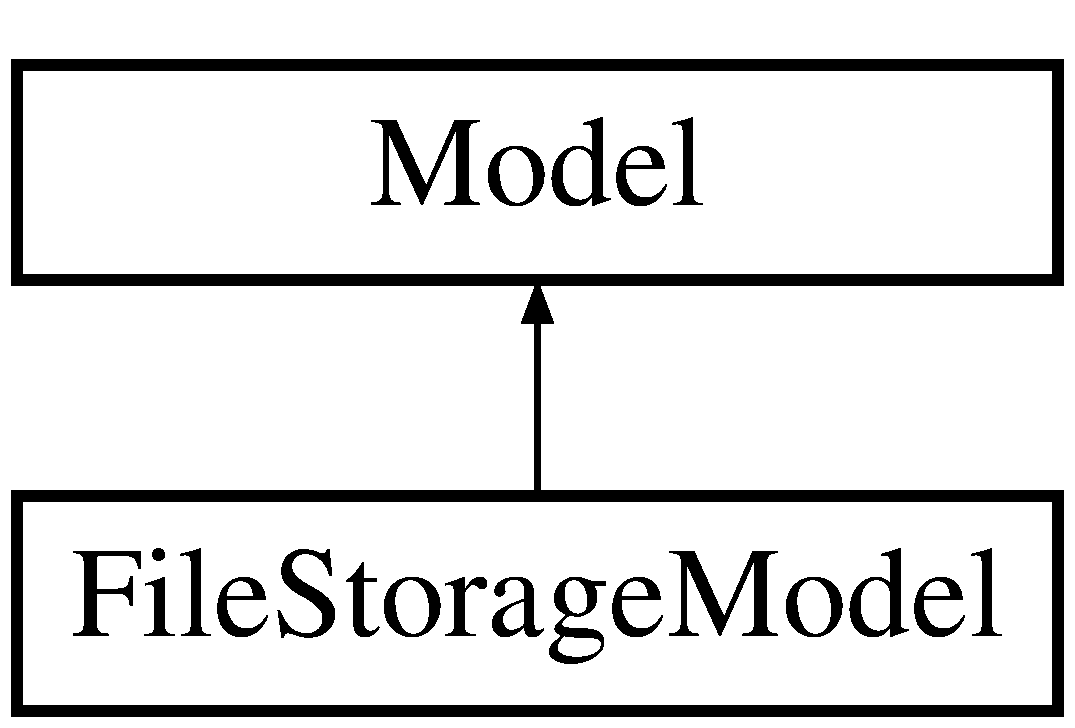
\includegraphics[height=2.000000cm]{class_file_storage_model}
\end{center}
\end{figure}
\subsection*{Public Member Functions}
\begin{DoxyCompactItemize}
\item 
\hyperlink{class_file_storage_model_a4a9563fed1ae1a659466d64ee8890653}{File\-Storage\-Model} ()
\item 
virtual \hyperlink{class_file_storage_model_aba448d7c91c33e63cdfc95c8580fd834}{$\sim$\-File\-Storage\-Model} ()
\item 
bool \hyperlink{class_file_storage_model_af97e8cf0ced06893ffca6ec119a31143}{deserialize} (const std\-::string \&filename)
\item 
bool \hyperlink{class_file_storage_model_acc945cf6792663f84f1302e926dca63d}{serialize} (const std\-::string \&filename) const 
\end{DoxyCompactItemize}
\subsection*{Additional Inherited Members}


\subsection{Detailed Description}
\hyperlink{class_model}{Model} with cv\-::\-File\-Storage (de-\/)serialization. 

\subsection{Constructor \& Destructor Documentation}
\hypertarget{class_file_storage_model_a4a9563fed1ae1a659466d64ee8890653}{\index{File\-Storage\-Model@{File\-Storage\-Model}!File\-Storage\-Model@{File\-Storage\-Model}}
\index{File\-Storage\-Model@{File\-Storage\-Model}!FileStorageModel@{File\-Storage\-Model}}
\subsubsection[{File\-Storage\-Model}]{\setlength{\rightskip}{0pt plus 5cm}File\-Storage\-Model\-::\-File\-Storage\-Model (
\begin{DoxyParamCaption}
{}
\end{DoxyParamCaption}
)\hspace{0.3cm}{\ttfamily [inline]}}}\label{class_file_storage_model_a4a9563fed1ae1a659466d64ee8890653}
\hypertarget{class_file_storage_model_aba448d7c91c33e63cdfc95c8580fd834}{\index{File\-Storage\-Model@{File\-Storage\-Model}!$\sim$\-File\-Storage\-Model@{$\sim$\-File\-Storage\-Model}}
\index{$\sim$\-File\-Storage\-Model@{$\sim$\-File\-Storage\-Model}!FileStorageModel@{File\-Storage\-Model}}
\subsubsection[{$\sim$\-File\-Storage\-Model}]{\setlength{\rightskip}{0pt plus 5cm}virtual File\-Storage\-Model\-::$\sim$\-File\-Storage\-Model (
\begin{DoxyParamCaption}
{}
\end{DoxyParamCaption}
)\hspace{0.3cm}{\ttfamily [inline]}, {\ttfamily [virtual]}}}\label{class_file_storage_model_aba448d7c91c33e63cdfc95c8580fd834}


\subsection{Member Function Documentation}
\hypertarget{class_file_storage_model_af97e8cf0ced06893ffca6ec119a31143}{\index{File\-Storage\-Model@{File\-Storage\-Model}!deserialize@{deserialize}}
\index{deserialize@{deserialize}!FileStorageModel@{File\-Storage\-Model}}
\subsubsection[{deserialize}]{\setlength{\rightskip}{0pt plus 5cm}bool File\-Storage\-Model\-::deserialize (
\begin{DoxyParamCaption}
\item[{const std\-::string \&}]{filename}
\end{DoxyParamCaption}
)\hspace{0.3cm}{\ttfamily [virtual]}}}\label{class_file_storage_model_af97e8cf0ced06893ffca6ec119a31143}


Implements \hyperlink{class_model_a2fc5d668c4930e8172e1a1460a8e6b46}{Model}.

\hypertarget{class_file_storage_model_acc945cf6792663f84f1302e926dca63d}{\index{File\-Storage\-Model@{File\-Storage\-Model}!serialize@{serialize}}
\index{serialize@{serialize}!FileStorageModel@{File\-Storage\-Model}}
\subsubsection[{serialize}]{\setlength{\rightskip}{0pt plus 5cm}bool File\-Storage\-Model\-::serialize (
\begin{DoxyParamCaption}
\item[{const std\-::string \&}]{filename}
\end{DoxyParamCaption}
) const\hspace{0.3cm}{\ttfamily [virtual]}}}\label{class_file_storage_model_acc945cf6792663f84f1302e926dca63d}


Implements \hyperlink{class_model_a952f21d72d87aa30387ea6e5c1d603fd}{Model}.



The documentation for this class was generated from the following files\-:\begin{DoxyCompactItemize}
\item 
/\-Users/m29474/\-Desktop/code/openbr/3rdparty/\-Parts\-Based\-Detector/include/\hyperlink{_file_storage_model_8hpp}{File\-Storage\-Model.\-hpp}\item 
/\-Users/m29474/\-Desktop/code/openbr/3rdparty/\-Parts\-Based\-Detector/src/\hyperlink{_file_storage_model_8cpp}{File\-Storage\-Model.\-cpp}\end{DoxyCompactItemize}

\hypertarget{class_fourier_convolution_engine}{\section{Fourier\-Convolution\-Engine Class Reference}
\label{class_fourier_convolution_engine}\index{Fourier\-Convolution\-Engine@{Fourier\-Convolution\-Engine}}
}


{\ttfamily \#include $<$Fourier\-Convolution\-Engine.\-hpp$>$}

Inheritance diagram for Fourier\-Convolution\-Engine\-:\begin{figure}[H]
\begin{center}
\leavevmode
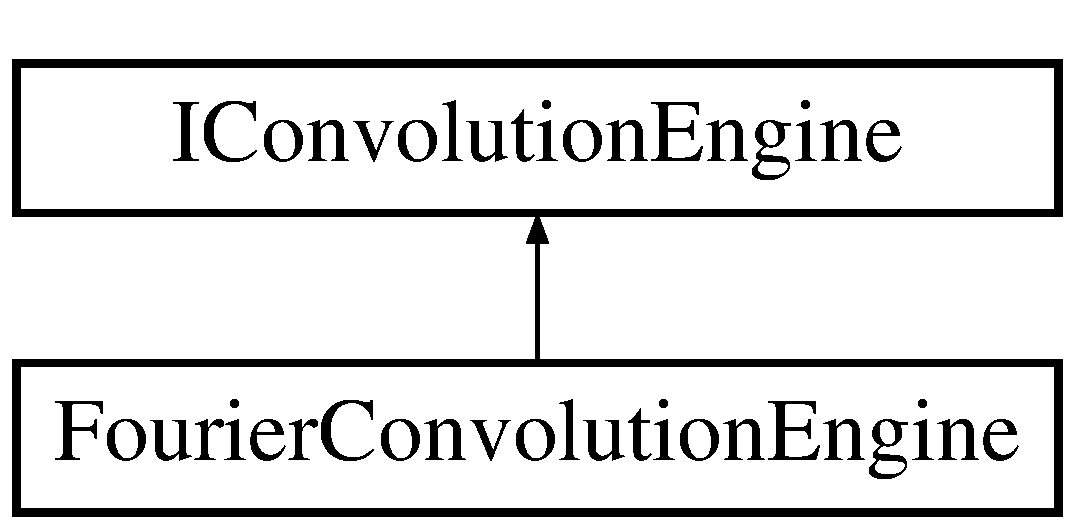
\includegraphics[height=2.000000cm]{class_fourier_convolution_engine}
\end{center}
\end{figure}
\subsection*{Public Member Functions}
\begin{DoxyCompactItemize}
\item 
\hyperlink{class_fourier_convolution_engine_a30d60a44b5767b43a4042171cf813fcd}{Fourier\-Convolution\-Engine} (const cv\-::\-Size \&size, int type, size\-\_\-t flen)
\item 
virtual \hyperlink{class_fourier_convolution_engine_a827dafdecfbb07891fbeee998af60236}{$\sim$\-Fourier\-Convolution\-Engine} ()
\item 
virtual void \hyperlink{class_fourier_convolution_engine_ad895979797d38a7c97e8dfcca9571fd2}{set\-Filters} (const \hyperlink{types_8hpp_a3207a7addcfa415d1c83622febcb1e9b}{vector\-Mat} \&filters)
\begin{DoxyCompactList}\small\item\em set the filters \end{DoxyCompactList}\item 
virtual void \hyperlink{class_fourier_convolution_engine_a30e84c8f67a198d318780e247efbbe41}{pdf} (const \hyperlink{types_8hpp_a3207a7addcfa415d1c83622febcb1e9b}{vector\-Mat} \&features, \hyperlink{types_8hpp_a33cacb85be7b8df3dc0b67d5d849f4cc}{vector2\-D\-Mat} \&responses)
\begin{DoxyCompactList}\small\item\em Calculate the responses of a set of features to a set of filter experts. \end{DoxyCompactList}\end{DoxyCompactItemize}
\subsection*{Private Member Functions}
\begin{DoxyCompactItemize}
\item 
void \hyperlink{class_fourier_convolution_engine_aaa0df468a2857c391459d3c9a53a6fc6}{convolve} (const cv\-::\-Mat \&feature, \hyperlink{types_8hpp_a3207a7addcfa415d1c83622febcb1e9b}{vector\-Mat} \&filter, cv\-::\-Mat \&\hyperlink{class_fourier_convolution_engine_a30e84c8f67a198d318780e247efbbe41}{pdf}, const size\-\_\-t channels)
\end{DoxyCompactItemize}
\subsection*{Private Attributes}
\begin{DoxyCompactItemize}
\item 
cv\-::\-Size \hyperlink{class_fourier_convolution_engine_a2375ea1729ad2fe45fe6204130f3f39f}{size\-\_\-}
\begin{DoxyCompactList}\small\item\em the largest expected image size \end{DoxyCompactList}\item 
int \hyperlink{class_fourier_convolution_engine_a3e213d98d690b295eaa2866618f17933}{type\-\_\-}
\begin{DoxyCompactList}\small\item\em the internally supported convolution type, taken from the filter type \end{DoxyCompactList}\item 
size\-\_\-t \hyperlink{class_fourier_convolution_engine_ab4322f51ce4a18ab5b7439abb5c96aef}{flen\-\_\-}
\begin{DoxyCompactList}\small\item\em the number of layers to each filter \end{DoxyCompactList}\item 
\hyperlink{types_8hpp_a33cacb85be7b8df3dc0b67d5d849f4cc}{vector2\-D\-Mat} \hyperlink{class_fourier_convolution_engine_ac6cf3c6a66e99bec7d8135f8069d79e3}{filters\-\_\-}
\begin{DoxyCompactList}\small\item\em the internal representation of the filters \end{DoxyCompactList}\end{DoxyCompactItemize}


\subsection{Constructor \& Destructor Documentation}
\hypertarget{class_fourier_convolution_engine_a30d60a44b5767b43a4042171cf813fcd}{\index{Fourier\-Convolution\-Engine@{Fourier\-Convolution\-Engine}!Fourier\-Convolution\-Engine@{Fourier\-Convolution\-Engine}}
\index{Fourier\-Convolution\-Engine@{Fourier\-Convolution\-Engine}!FourierConvolutionEngine@{Fourier\-Convolution\-Engine}}
\subsubsection[{Fourier\-Convolution\-Engine}]{\setlength{\rightskip}{0pt plus 5cm}Fourier\-Convolution\-Engine\-::\-Fourier\-Convolution\-Engine (
\begin{DoxyParamCaption}
\item[{const cv\-::\-Size \&}]{size, }
\item[{int}]{type, }
\item[{size\-\_\-t}]{flen}
\end{DoxyParamCaption}
)}}\label{class_fourier_convolution_engine_a30d60a44b5767b43a4042171cf813fcd}
\hypertarget{class_fourier_convolution_engine_a827dafdecfbb07891fbeee998af60236}{\index{Fourier\-Convolution\-Engine@{Fourier\-Convolution\-Engine}!$\sim$\-Fourier\-Convolution\-Engine@{$\sim$\-Fourier\-Convolution\-Engine}}
\index{$\sim$\-Fourier\-Convolution\-Engine@{$\sim$\-Fourier\-Convolution\-Engine}!FourierConvolutionEngine@{Fourier\-Convolution\-Engine}}
\subsubsection[{$\sim$\-Fourier\-Convolution\-Engine}]{\setlength{\rightskip}{0pt plus 5cm}Fourier\-Convolution\-Engine\-::$\sim$\-Fourier\-Convolution\-Engine (
\begin{DoxyParamCaption}
{}
\end{DoxyParamCaption}
)\hspace{0.3cm}{\ttfamily [virtual]}}}\label{class_fourier_convolution_engine_a827dafdecfbb07891fbeee998af60236}


\subsection{Member Function Documentation}
\hypertarget{class_fourier_convolution_engine_aaa0df468a2857c391459d3c9a53a6fc6}{\index{Fourier\-Convolution\-Engine@{Fourier\-Convolution\-Engine}!convolve@{convolve}}
\index{convolve@{convolve}!FourierConvolutionEngine@{Fourier\-Convolution\-Engine}}
\subsubsection[{convolve}]{\setlength{\rightskip}{0pt plus 5cm}void Fourier\-Convolution\-Engine\-::convolve (
\begin{DoxyParamCaption}
\item[{const cv\-::\-Mat \&}]{feature, }
\item[{{\bf vector\-Mat} \&}]{filter, }
\item[{cv\-::\-Mat \&}]{pdf, }
\item[{const size\-\_\-t}]{channels}
\end{DoxyParamCaption}
)\hspace{0.3cm}{\ttfamily [private]}}}\label{class_fourier_convolution_engine_aaa0df468a2857c391459d3c9a53a6fc6}
\hypertarget{class_fourier_convolution_engine_a30e84c8f67a198d318780e247efbbe41}{\index{Fourier\-Convolution\-Engine@{Fourier\-Convolution\-Engine}!pdf@{pdf}}
\index{pdf@{pdf}!FourierConvolutionEngine@{Fourier\-Convolution\-Engine}}
\subsubsection[{pdf}]{\setlength{\rightskip}{0pt plus 5cm}void Fourier\-Convolution\-Engine\-::pdf (
\begin{DoxyParamCaption}
\item[{const {\bf vector\-Mat} \&}]{features, }
\item[{{\bf vector2\-D\-Mat} \&}]{responses}
\end{DoxyParamCaption}
)\hspace{0.3cm}{\ttfamily [virtual]}}}\label{class_fourier_convolution_engine_a30e84c8f67a198d318780e247efbbe41}


Calculate the responses of a set of features to a set of filter experts. 

A response represents the likelihood of the part appearing at each location of the feature map. \hyperlink{class_parts}{Parts} are support vector machines (S\-V\-Ms) represented as filters. The convolution of a filter with a feature produces a probability density function (pdf) of part location 
\begin{DoxyParams}{Parameters}
{\em features} & the input features (at different scales, and by extension, size) \\
\hline
{\em responses} & the vector of responses (pdfs) to return \\
\hline
\end{DoxyParams}


Implements \hyperlink{class_i_convolution_engine_ab5aaabb634629a714d397a6c1a9c9400}{I\-Convolution\-Engine}.

\hypertarget{class_fourier_convolution_engine_ad895979797d38a7c97e8dfcca9571fd2}{\index{Fourier\-Convolution\-Engine@{Fourier\-Convolution\-Engine}!set\-Filters@{set\-Filters}}
\index{set\-Filters@{set\-Filters}!FourierConvolutionEngine@{Fourier\-Convolution\-Engine}}
\subsubsection[{set\-Filters}]{\setlength{\rightskip}{0pt plus 5cm}void Fourier\-Convolution\-Engine\-::set\-Filters (
\begin{DoxyParamCaption}
\item[{const {\bf vector\-Mat} \&}]{filters}
\end{DoxyParamCaption}
)\hspace{0.3cm}{\ttfamily [virtual]}}}\label{class_fourier_convolution_engine_ad895979797d38a7c97e8dfcca9571fd2}


set the filters 

given a set of filters, split each filter channel into a plane, in preparation for convolution


\begin{DoxyParams}{Parameters}
{\em filters} & the filters \\
\hline
\end{DoxyParams}


Implements \hyperlink{class_i_convolution_engine_a3570aae351b5fcb93bcd87a06c65ea0a}{I\-Convolution\-Engine}.



\subsection{Field Documentation}
\hypertarget{class_fourier_convolution_engine_ac6cf3c6a66e99bec7d8135f8069d79e3}{\index{Fourier\-Convolution\-Engine@{Fourier\-Convolution\-Engine}!filters\-\_\-@{filters\-\_\-}}
\index{filters\-\_\-@{filters\-\_\-}!FourierConvolutionEngine@{Fourier\-Convolution\-Engine}}
\subsubsection[{filters\-\_\-}]{\setlength{\rightskip}{0pt plus 5cm}{\bf vector2\-D\-Mat} Fourier\-Convolution\-Engine\-::filters\-\_\-\hspace{0.3cm}{\ttfamily [private]}}}\label{class_fourier_convolution_engine_ac6cf3c6a66e99bec7d8135f8069d79e3}


the internal representation of the filters 

\hypertarget{class_fourier_convolution_engine_ab4322f51ce4a18ab5b7439abb5c96aef}{\index{Fourier\-Convolution\-Engine@{Fourier\-Convolution\-Engine}!flen\-\_\-@{flen\-\_\-}}
\index{flen\-\_\-@{flen\-\_\-}!FourierConvolutionEngine@{Fourier\-Convolution\-Engine}}
\subsubsection[{flen\-\_\-}]{\setlength{\rightskip}{0pt plus 5cm}size\-\_\-t Fourier\-Convolution\-Engine\-::flen\-\_\-\hspace{0.3cm}{\ttfamily [private]}}}\label{class_fourier_convolution_engine_ab4322f51ce4a18ab5b7439abb5c96aef}


the number of layers to each filter 

\hypertarget{class_fourier_convolution_engine_a2375ea1729ad2fe45fe6204130f3f39f}{\index{Fourier\-Convolution\-Engine@{Fourier\-Convolution\-Engine}!size\-\_\-@{size\-\_\-}}
\index{size\-\_\-@{size\-\_\-}!FourierConvolutionEngine@{Fourier\-Convolution\-Engine}}
\subsubsection[{size\-\_\-}]{\setlength{\rightskip}{0pt plus 5cm}cv\-::\-Size Fourier\-Convolution\-Engine\-::size\-\_\-\hspace{0.3cm}{\ttfamily [private]}}}\label{class_fourier_convolution_engine_a2375ea1729ad2fe45fe6204130f3f39f}


the largest expected image size 

\hypertarget{class_fourier_convolution_engine_a3e213d98d690b295eaa2866618f17933}{\index{Fourier\-Convolution\-Engine@{Fourier\-Convolution\-Engine}!type\-\_\-@{type\-\_\-}}
\index{type\-\_\-@{type\-\_\-}!FourierConvolutionEngine@{Fourier\-Convolution\-Engine}}
\subsubsection[{type\-\_\-}]{\setlength{\rightskip}{0pt plus 5cm}int Fourier\-Convolution\-Engine\-::type\-\_\-\hspace{0.3cm}{\ttfamily [private]}}}\label{class_fourier_convolution_engine_a3e213d98d690b295eaa2866618f17933}


the internally supported convolution type, taken from the filter type 



The documentation for this class was generated from the following files\-:\begin{DoxyCompactItemize}
\item 
/\-Users/m29474/\-Desktop/code/openbr/3rdparty/\-Parts\-Based\-Detector/include/\hyperlink{_fourier_convolution_engine_8hpp}{Fourier\-Convolution\-Engine.\-hpp}\item 
/\-Users/m29474/\-Desktop/code/openbr/3rdparty/\-Parts\-Based\-Detector/src/\hyperlink{_fourier_convolution_engine_8cpp}{Fourier\-Convolution\-Engine.\-cpp}\end{DoxyCompactItemize}

\hypertarget{class_h_o_g_features}{\section{H\-O\-G\-Features$<$ T $>$ Class Template Reference}
\label{class_h_o_g_features}\index{H\-O\-G\-Features$<$ T $>$@{H\-O\-G\-Features$<$ T $>$}}
}


Implementation of \hyperlink{class_i_features}{I\-Features} interface using H\-O\-G.  




{\ttfamily \#include $<$H\-O\-G\-Features.\-hpp$>$}

Inheritance diagram for H\-O\-G\-Features$<$ T $>$\-:\begin{figure}[H]
\begin{center}
\leavevmode
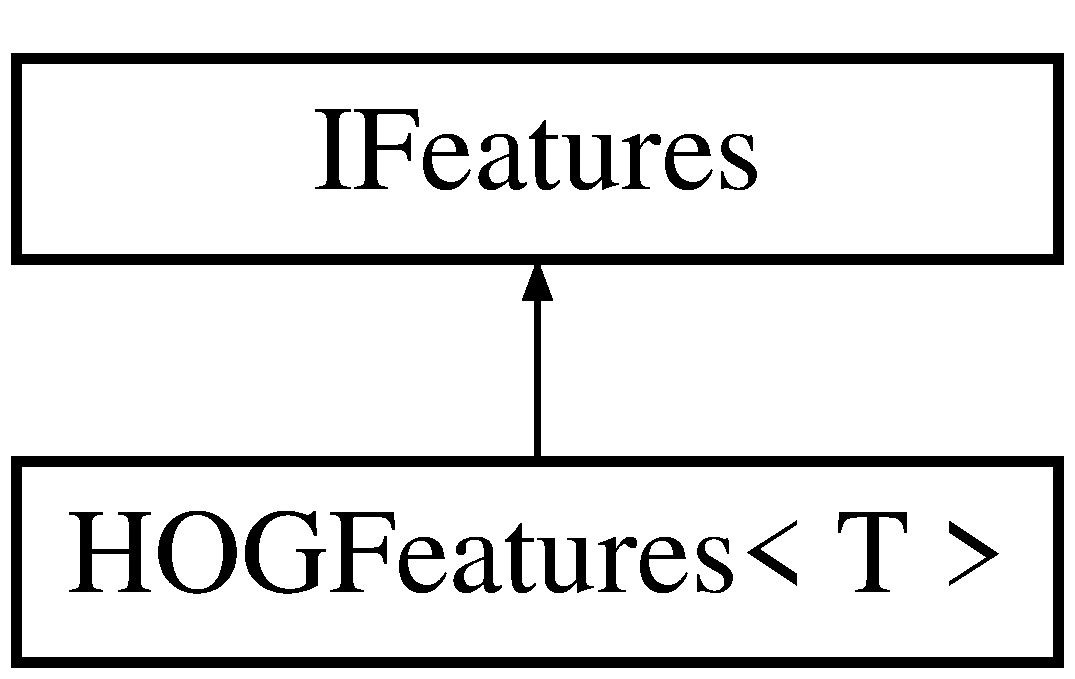
\includegraphics[height=2.000000cm]{class_h_o_g_features}
\end{center}
\end{figure}
\subsection*{Public Member Functions}
\begin{DoxyCompactItemize}
\item 
\hyperlink{class_h_o_g_features_a323944dc2065bfb4d7b83bac6ea0ba69}{H\-O\-G\-Features} ()
\item 
\hyperlink{class_h_o_g_features_aac660f7db27da50fc026e6e25b374b5a}{H\-O\-G\-Features} (size\-\_\-t \hyperlink{class_h_o_g_features_a0b75015646ceac02ba250e5af86245d4}{binsize}, size\-\_\-t \hyperlink{class_h_o_g_features_a2ea95a95f6d79af3344502b45e1cb7c5}{nscales}, size\-\_\-t flen, size\-\_\-t norient)
\item 
virtual \hyperlink{class_h_o_g_features_a062d1cfbb82dbd2829e844a937490509}{$\sim$\-H\-O\-G\-Features} ()
\item 
size\-\_\-t \hyperlink{class_h_o_g_features_a0b75015646ceac02ba250e5af86245d4}{binsize} (void) const 
\begin{DoxyCompactList}\small\item\em retrieve the spatial binning size (1 if not relevant) \end{DoxyCompactList}\item 
size\-\_\-t \hyperlink{class_h_o_g_features_a2ea95a95f6d79af3344502b45e1cb7c5}{nscales} (void) const 
\begin{DoxyCompactList}\small\item\em retrieve the number of scales the features are calculated over \end{DoxyCompactList}\item 
\hyperlink{types_8hpp_a4da5db3ee9e284f719ef5764dbadffc8}{vectorf} \hyperlink{class_h_o_g_features_ad9668fda860881c676e1d1bd70adc18c}{scales} (void) const 
\begin{DoxyCompactList}\small\item\em the vector of scales \end{DoxyCompactList}\item 
void \hyperlink{class_h_o_g_features_a509372c4e652c3fc97f2d2be75fecd4d}{pyramid} (const cv\-::\-Mat \&im, \hyperlink{types_8hpp_a3207a7addcfa415d1c83622febcb1e9b}{vector\-Mat} \&pyrafeatures)
\begin{DoxyCompactList}\small\item\em Calculate features at multiple scales. \end{DoxyCompactList}\item 
{\footnotesize template$<$typename I\-T $>$ }\\void \hyperlink{class_h_o_g_features_a0cabf74792b44e23e3dfd2c388b12036}{features} (const Mat \&imm, Mat \&featm) const 
\begin{DoxyCompactList}\small\item\em compute the H\-O\-G features for an image \end{DoxyCompactList}\end{DoxyCompactItemize}
\subsection*{Private Member Functions}
\begin{DoxyCompactItemize}
\item 
void \hyperlink{class_h_o_g_features_aef691ef9b65758f54b5b18dc496544b4}{boundary\-Occlusion\-Feature} (cv\-::\-Mat \&feature, const int flen, const int padsize)
\begin{DoxyCompactList}\small\item\em add ones to the final padded pixel in each 3\-D feature map \end{DoxyCompactList}\item 
{\footnotesize template$<$typename I\-T $>$ }\\void \hyperlink{class_h_o_g_features_a1283b0cdf821061a4195de479e854199}{features} (const cv\-::\-Mat \&im, cv\-::\-Mat \&feature) const 
\end{DoxyCompactItemize}
\subsection*{Private Attributes}
\begin{DoxyCompactItemize}
\item 
size\-\_\-t \hyperlink{class_h_o_g_features_afd93266461d3389e4c61a9c06fc81f4f}{binsize\-\_\-}
\begin{DoxyCompactList}\small\item\em the spatial binning size \end{DoxyCompactList}\item 
size\-\_\-t \hyperlink{class_h_o_g_features_a46cde43950d00f33de7d11cd8a8da5bf}{nscales\-\_\-}
\begin{DoxyCompactList}\small\item\em the number of scales to compute features at \end{DoxyCompactList}\item 
size\-\_\-t \hyperlink{class_h_o_g_features_a8cf4e36a70e13230efbe8abe97928748}{flen\-\_\-}
\begin{DoxyCompactList}\small\item\em the length of the feature at each bin (histogram size) \end{DoxyCompactList}\item 
size\-\_\-t \hyperlink{class_h_o_g_features_a2c2f06c85eed3a2b2f93574116b961f7}{norient\-\_\-}
\begin{DoxyCompactList}\small\item\em the number of orientations to bin \end{DoxyCompactList}\item 
\hyperlink{types_8hpp_a4da5db3ee9e284f719ef5764dbadffc8}{vectorf} \hyperlink{class_h_o_g_features_a27490a8c33c7ffbfdeedafc5af0ad544}{scales\-\_\-}
\begin{DoxyCompactList}\small\item\em the scales of the features \end{DoxyCompactList}\item 
float \hyperlink{class_h_o_g_features_a45b232ca94e93b4f30d342374e62578f}{sfactor\-\_\-}
\begin{DoxyCompactList}\small\item\em the scaling factor between successive levels in the pyramid \end{DoxyCompactList}\item 
size\-\_\-t \hyperlink{class_h_o_g_features_aaa063fbfe2ce734ee08a10d7292cfb54}{interval\-\_\-}
\begin{DoxyCompactList}\small\item\em the interval between half resolution scales \end{DoxyCompactList}\end{DoxyCompactItemize}


\subsection{Detailed Description}
\subsubsection*{template$<$typename T$>$class H\-O\-G\-Features$<$ T $>$}

Implementation of \hyperlink{class_i_features}{I\-Features} interface using H\-O\-G. 

\subsection{Constructor \& Destructor Documentation}
\hypertarget{class_h_o_g_features_a323944dc2065bfb4d7b83bac6ea0ba69}{\index{H\-O\-G\-Features@{H\-O\-G\-Features}!H\-O\-G\-Features@{H\-O\-G\-Features}}
\index{H\-O\-G\-Features@{H\-O\-G\-Features}!HOGFeatures@{H\-O\-G\-Features}}
\subsubsection[{H\-O\-G\-Features}]{\setlength{\rightskip}{0pt plus 5cm}template$<$typename T $>$ {\bf H\-O\-G\-Features}$<$ T $>$\-::{\bf H\-O\-G\-Features} (
\begin{DoxyParamCaption}
{}
\end{DoxyParamCaption}
)\hspace{0.3cm}{\ttfamily [inline]}}}\label{class_h_o_g_features_a323944dc2065bfb4d7b83bac6ea0ba69}
\hypertarget{class_h_o_g_features_aac660f7db27da50fc026e6e25b374b5a}{\index{H\-O\-G\-Features@{H\-O\-G\-Features}!H\-O\-G\-Features@{H\-O\-G\-Features}}
\index{H\-O\-G\-Features@{H\-O\-G\-Features}!HOGFeatures@{H\-O\-G\-Features}}
\subsubsection[{H\-O\-G\-Features}]{\setlength{\rightskip}{0pt plus 5cm}template$<$typename T $>$ {\bf H\-O\-G\-Features}$<$ T $>$\-::{\bf H\-O\-G\-Features} (
\begin{DoxyParamCaption}
\item[{size\-\_\-t}]{binsize, }
\item[{size\-\_\-t}]{nscales, }
\item[{size\-\_\-t}]{flen, }
\item[{size\-\_\-t}]{norient}
\end{DoxyParamCaption}
)\hspace{0.3cm}{\ttfamily [inline]}}}\label{class_h_o_g_features_aac660f7db27da50fc026e6e25b374b5a}
\hypertarget{class_h_o_g_features_a062d1cfbb82dbd2829e844a937490509}{\index{H\-O\-G\-Features@{H\-O\-G\-Features}!$\sim$\-H\-O\-G\-Features@{$\sim$\-H\-O\-G\-Features}}
\index{$\sim$\-H\-O\-G\-Features@{$\sim$\-H\-O\-G\-Features}!HOGFeatures@{H\-O\-G\-Features}}
\subsubsection[{$\sim$\-H\-O\-G\-Features}]{\setlength{\rightskip}{0pt plus 5cm}template$<$typename T $>$ virtual {\bf H\-O\-G\-Features}$<$ T $>$\-::$\sim${\bf H\-O\-G\-Features} (
\begin{DoxyParamCaption}
{}
\end{DoxyParamCaption}
)\hspace{0.3cm}{\ttfamily [inline]}, {\ttfamily [virtual]}}}\label{class_h_o_g_features_a062d1cfbb82dbd2829e844a937490509}


\subsection{Member Function Documentation}
\hypertarget{class_h_o_g_features_a0b75015646ceac02ba250e5af86245d4}{\index{H\-O\-G\-Features@{H\-O\-G\-Features}!binsize@{binsize}}
\index{binsize@{binsize}!HOGFeatures@{H\-O\-G\-Features}}
\subsubsection[{binsize}]{\setlength{\rightskip}{0pt plus 5cm}template$<$typename T $>$ size\-\_\-t {\bf H\-O\-G\-Features}$<$ T $>$\-::binsize (
\begin{DoxyParamCaption}
\item[{void}]{}
\end{DoxyParamCaption}
) const\hspace{0.3cm}{\ttfamily [inline]}, {\ttfamily [virtual]}}}\label{class_h_o_g_features_a0b75015646ceac02ba250e5af86245d4}


retrieve the spatial binning size (1 if not relevant) 



Implements \hyperlink{class_i_features_a79f6861190d7c2754d560c6c10baa787}{I\-Features}.

\hypertarget{class_h_o_g_features_aef691ef9b65758f54b5b18dc496544b4}{\index{H\-O\-G\-Features@{H\-O\-G\-Features}!boundary\-Occlusion\-Feature@{boundary\-Occlusion\-Feature}}
\index{boundary\-Occlusion\-Feature@{boundary\-Occlusion\-Feature}!HOGFeatures@{H\-O\-G\-Features}}
\subsubsection[{boundary\-Occlusion\-Feature}]{\setlength{\rightskip}{0pt plus 5cm}template$<$typename T $>$ void {\bf H\-O\-G\-Features}$<$ T $>$\-::boundary\-Occlusion\-Feature (
\begin{DoxyParamCaption}
\item[{cv\-::\-Mat \&}]{feature, }
\item[{const int}]{flen, }
\item[{const int}]{padsize}
\end{DoxyParamCaption}
)\hspace{0.3cm}{\ttfamily [private]}}}\label{class_h_o_g_features_aef691ef9b65758f54b5b18dc496544b4}


add ones to the final padded pixel in each 3\-D feature map 


\begin{DoxyParams}{Parameters}
{\em feature} & the feature map \\
\hline
{\em flen} & the length of the feature \\
\hline
{\em padsize} & the amount of padding that was applied (equally to all dimensions) \\
\hline
\end{DoxyParams}
\hypertarget{class_h_o_g_features_a1283b0cdf821061a4195de479e854199}{\index{H\-O\-G\-Features@{H\-O\-G\-Features}!features@{features}}
\index{features@{features}!HOGFeatures@{H\-O\-G\-Features}}
\subsubsection[{features}]{\setlength{\rightskip}{0pt plus 5cm}template$<$typename T $>$ template$<$typename I\-T $>$ void {\bf H\-O\-G\-Features}$<$ T $>$\-::features (
\begin{DoxyParamCaption}
\item[{const cv\-::\-Mat \&}]{im, }
\item[{cv\-::\-Mat \&}]{feature}
\end{DoxyParamCaption}
) const\hspace{0.3cm}{\ttfamily [private]}}}\label{class_h_o_g_features_a1283b0cdf821061a4195de479e854199}
\hypertarget{class_h_o_g_features_a0cabf74792b44e23e3dfd2c388b12036}{\index{H\-O\-G\-Features@{H\-O\-G\-Features}!features@{features}}
\index{features@{features}!HOGFeatures@{H\-O\-G\-Features}}
\subsubsection[{features}]{\setlength{\rightskip}{0pt plus 5cm}template$<$typename T $>$ template$<$typename I\-T $>$ void {\bf H\-O\-G\-Features}$<$ T $>$\-::features (
\begin{DoxyParamCaption}
\item[{const Mat \&}]{imm, }
\item[{Mat \&}]{featm}
\end{DoxyParamCaption}
) const}}\label{class_h_o_g_features_a0cabf74792b44e23e3dfd2c388b12036}


compute the H\-O\-G features for an image 

This method computes the H\-O\-G features for an image, given the binsize\-\_\- and flen\-\_\- class members. The output is effectively a 3\-D matrix (i,j,k) that has been flattened to a 2\-D (i,j$\ast$k) matrix for faster processing. The (i,j) dimensions represent the resultant spatial size of the response (ie im.\-size() / binsize\-\_\-) and the (k) dimension represents the histogram weights (length flen\-\_\-)

The function supports multithreading via Open\-M\-P


\begin{DoxyParams}{Parameters}
{\em imm} & the input image (must be color of type C\-V\-\_\-8\-U\-C3) \\
\hline
{\em featm} & the H\-O\-G features as a 2\-D matrix \\
\hline
\end{DoxyParams}
\hypertarget{class_h_o_g_features_a2ea95a95f6d79af3344502b45e1cb7c5}{\index{H\-O\-G\-Features@{H\-O\-G\-Features}!nscales@{nscales}}
\index{nscales@{nscales}!HOGFeatures@{H\-O\-G\-Features}}
\subsubsection[{nscales}]{\setlength{\rightskip}{0pt plus 5cm}template$<$typename T $>$ size\-\_\-t {\bf H\-O\-G\-Features}$<$ T $>$\-::nscales (
\begin{DoxyParamCaption}
\item[{void}]{}
\end{DoxyParamCaption}
) const\hspace{0.3cm}{\ttfamily [inline]}, {\ttfamily [virtual]}}}\label{class_h_o_g_features_a2ea95a95f6d79af3344502b45e1cb7c5}


retrieve the number of scales the features are calculated over 



Implements \hyperlink{class_i_features_abf8d0bf5f66e7b3188ca73b5c9e48a1f}{I\-Features}.

\hypertarget{class_h_o_g_features_a509372c4e652c3fc97f2d2be75fecd4d}{\index{H\-O\-G\-Features@{H\-O\-G\-Features}!pyramid@{pyramid}}
\index{pyramid@{pyramid}!HOGFeatures@{H\-O\-G\-Features}}
\subsubsection[{pyramid}]{\setlength{\rightskip}{0pt plus 5cm}template$<$typename T $>$ void {\bf H\-O\-G\-Features}$<$ T $>$\-::pyramid (
\begin{DoxyParamCaption}
\item[{const cv\-::\-Mat \&}]{im, }
\item[{{\bf vector\-Mat} \&}]{pyrafeatures}
\end{DoxyParamCaption}
)\hspace{0.3cm}{\ttfamily [virtual]}}}\label{class_h_o_g_features_a509372c4e652c3fc97f2d2be75fecd4d}


Calculate features at multiple scales. 

Features are calculated first at native resolution, then progressively downsampled to coarser spatial resolutions

This function supports multithreading via Open\-M\-P


\begin{DoxyParams}{Parameters}
{\em im} & the input image at native resolution \\
\hline
{\em pyrafeatures} & the pyramid of features, fine to coarse, each calculated via \hyperlink{class_h_o_g_features_a1283b0cdf821061a4195de479e854199}{features()} \\
\hline
\end{DoxyParams}


Implements \hyperlink{class_i_features_a0cd270503671145fae965c8d9fedc91a}{I\-Features}.

\hypertarget{class_h_o_g_features_ad9668fda860881c676e1d1bd70adc18c}{\index{H\-O\-G\-Features@{H\-O\-G\-Features}!scales@{scales}}
\index{scales@{scales}!HOGFeatures@{H\-O\-G\-Features}}
\subsubsection[{scales}]{\setlength{\rightskip}{0pt plus 5cm}template$<$typename T $>$ {\bf vectorf} {\bf H\-O\-G\-Features}$<$ T $>$\-::scales (
\begin{DoxyParamCaption}
\item[{void}]{}
\end{DoxyParamCaption}
) const\hspace{0.3cm}{\ttfamily [inline]}, {\ttfamily [virtual]}}}\label{class_h_o_g_features_ad9668fda860881c676e1d1bd70adc18c}


the vector of scales 

the vector of scales, 1 indicating the native image resolution, values lower than 1 indicating downsampled images, and values greater than 1 indicating hallucinated resolutions 

Implements \hyperlink{class_i_features_ad02aea9fd29e438d25e1c7d68c508b9e}{I\-Features}.



\subsection{Field Documentation}
\hypertarget{class_h_o_g_features_afd93266461d3389e4c61a9c06fc81f4f}{\index{H\-O\-G\-Features@{H\-O\-G\-Features}!binsize\-\_\-@{binsize\-\_\-}}
\index{binsize\-\_\-@{binsize\-\_\-}!HOGFeatures@{H\-O\-G\-Features}}
\subsubsection[{binsize\-\_\-}]{\setlength{\rightskip}{0pt plus 5cm}template$<$typename T $>$ size\-\_\-t {\bf H\-O\-G\-Features}$<$ T $>$\-::binsize\-\_\-\hspace{0.3cm}{\ttfamily [private]}}}\label{class_h_o_g_features_afd93266461d3389e4c61a9c06fc81f4f}


the spatial binning size 

\hypertarget{class_h_o_g_features_a8cf4e36a70e13230efbe8abe97928748}{\index{H\-O\-G\-Features@{H\-O\-G\-Features}!flen\-\_\-@{flen\-\_\-}}
\index{flen\-\_\-@{flen\-\_\-}!HOGFeatures@{H\-O\-G\-Features}}
\subsubsection[{flen\-\_\-}]{\setlength{\rightskip}{0pt plus 5cm}template$<$typename T $>$ size\-\_\-t {\bf H\-O\-G\-Features}$<$ T $>$\-::flen\-\_\-\hspace{0.3cm}{\ttfamily [private]}}}\label{class_h_o_g_features_a8cf4e36a70e13230efbe8abe97928748}


the length of the feature at each bin (histogram size) 

\hypertarget{class_h_o_g_features_aaa063fbfe2ce734ee08a10d7292cfb54}{\index{H\-O\-G\-Features@{H\-O\-G\-Features}!interval\-\_\-@{interval\-\_\-}}
\index{interval\-\_\-@{interval\-\_\-}!HOGFeatures@{H\-O\-G\-Features}}
\subsubsection[{interval\-\_\-}]{\setlength{\rightskip}{0pt plus 5cm}template$<$typename T $>$ size\-\_\-t {\bf H\-O\-G\-Features}$<$ T $>$\-::interval\-\_\-\hspace{0.3cm}{\ttfamily [private]}}}\label{class_h_o_g_features_aaa063fbfe2ce734ee08a10d7292cfb54}


the interval between half resolution scales 

\hypertarget{class_h_o_g_features_a2c2f06c85eed3a2b2f93574116b961f7}{\index{H\-O\-G\-Features@{H\-O\-G\-Features}!norient\-\_\-@{norient\-\_\-}}
\index{norient\-\_\-@{norient\-\_\-}!HOGFeatures@{H\-O\-G\-Features}}
\subsubsection[{norient\-\_\-}]{\setlength{\rightskip}{0pt plus 5cm}template$<$typename T $>$ size\-\_\-t {\bf H\-O\-G\-Features}$<$ T $>$\-::norient\-\_\-\hspace{0.3cm}{\ttfamily [private]}}}\label{class_h_o_g_features_a2c2f06c85eed3a2b2f93574116b961f7}


the number of orientations to bin 

\hypertarget{class_h_o_g_features_a46cde43950d00f33de7d11cd8a8da5bf}{\index{H\-O\-G\-Features@{H\-O\-G\-Features}!nscales\-\_\-@{nscales\-\_\-}}
\index{nscales\-\_\-@{nscales\-\_\-}!HOGFeatures@{H\-O\-G\-Features}}
\subsubsection[{nscales\-\_\-}]{\setlength{\rightskip}{0pt plus 5cm}template$<$typename T $>$ size\-\_\-t {\bf H\-O\-G\-Features}$<$ T $>$\-::nscales\-\_\-\hspace{0.3cm}{\ttfamily [private]}}}\label{class_h_o_g_features_a46cde43950d00f33de7d11cd8a8da5bf}


the number of scales to compute features at 

\hypertarget{class_h_o_g_features_a27490a8c33c7ffbfdeedafc5af0ad544}{\index{H\-O\-G\-Features@{H\-O\-G\-Features}!scales\-\_\-@{scales\-\_\-}}
\index{scales\-\_\-@{scales\-\_\-}!HOGFeatures@{H\-O\-G\-Features}}
\subsubsection[{scales\-\_\-}]{\setlength{\rightskip}{0pt plus 5cm}template$<$typename T $>$ {\bf vectorf} {\bf H\-O\-G\-Features}$<$ T $>$\-::scales\-\_\-\hspace{0.3cm}{\ttfamily [private]}}}\label{class_h_o_g_features_a27490a8c33c7ffbfdeedafc5af0ad544}


the scales of the features 

\hypertarget{class_h_o_g_features_a45b232ca94e93b4f30d342374e62578f}{\index{H\-O\-G\-Features@{H\-O\-G\-Features}!sfactor\-\_\-@{sfactor\-\_\-}}
\index{sfactor\-\_\-@{sfactor\-\_\-}!HOGFeatures@{H\-O\-G\-Features}}
\subsubsection[{sfactor\-\_\-}]{\setlength{\rightskip}{0pt plus 5cm}template$<$typename T $>$ float {\bf H\-O\-G\-Features}$<$ T $>$\-::sfactor\-\_\-\hspace{0.3cm}{\ttfamily [private]}}}\label{class_h_o_g_features_a45b232ca94e93b4f30d342374e62578f}


the scaling factor between successive levels in the pyramid 



The documentation for this class was generated from the following files\-:\begin{DoxyCompactItemize}
\item 
/\-Users/m29474/\-Desktop/code/openbr/3rdparty/\-Parts\-Based\-Detector/include/\hyperlink{_h_o_g_features_8hpp}{H\-O\-G\-Features.\-hpp}\item 
/\-Users/m29474/\-Desktop/code/openbr/3rdparty/\-Parts\-Based\-Detector/src/\hyperlink{_h_o_g_features_8cpp}{H\-O\-G\-Features.\-cpp}\end{DoxyCompactItemize}

\hypertarget{class_i_convolution_engine}{\section{I\-Convolution\-Engine Class Reference}
\label{class_i_convolution_engine}\index{I\-Convolution\-Engine@{I\-Convolution\-Engine}}
}


{\ttfamily \#include $<$I\-Convolution\-Engine.\-hpp$>$}

Inheritance diagram for I\-Convolution\-Engine\-:\begin{figure}[H]
\begin{center}
\leavevmode
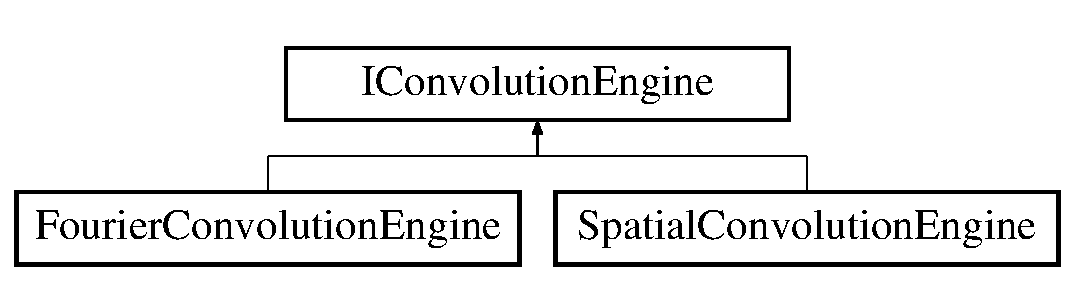
\includegraphics[height=2.000000cm]{class_i_convolution_engine}
\end{center}
\end{figure}
\subsection*{Public Member Functions}
\begin{DoxyCompactItemize}
\item 
virtual \hyperlink{class_i_convolution_engine_a554cb87e8dbd32552defd43549b9c1b3}{$\sim$\-I\-Convolution\-Engine} ()
\item 
virtual void \hyperlink{class_i_convolution_engine_ab5aaabb634629a714d397a6c1a9c9400}{pdf} (const \hyperlink{types_8hpp_a3207a7addcfa415d1c83622febcb1e9b}{vector\-Mat} \&features, \hyperlink{types_8hpp_a33cacb85be7b8df3dc0b67d5d849f4cc}{vector2\-D\-Mat} \&responses)=0
\begin{DoxyCompactList}\small\item\em probability density function \end{DoxyCompactList}\item 
virtual void \hyperlink{class_i_convolution_engine_a3570aae351b5fcb93bcd87a06c65ea0a}{set\-Filters} (const \hyperlink{types_8hpp_a3207a7addcfa415d1c83622febcb1e9b}{vector\-Mat} \&filters)=0
\begin{DoxyCompactList}\small\item\em set the convolve engine filters \end{DoxyCompactList}\end{DoxyCompactItemize}


\subsection{Constructor \& Destructor Documentation}
\hypertarget{class_i_convolution_engine_a554cb87e8dbd32552defd43549b9c1b3}{\index{I\-Convolution\-Engine@{I\-Convolution\-Engine}!$\sim$\-I\-Convolution\-Engine@{$\sim$\-I\-Convolution\-Engine}}
\index{$\sim$\-I\-Convolution\-Engine@{$\sim$\-I\-Convolution\-Engine}!IConvolutionEngine@{I\-Convolution\-Engine}}
\subsubsection[{$\sim$\-I\-Convolution\-Engine}]{\setlength{\rightskip}{0pt plus 5cm}virtual I\-Convolution\-Engine\-::$\sim$\-I\-Convolution\-Engine (
\begin{DoxyParamCaption}
{}
\end{DoxyParamCaption}
)\hspace{0.3cm}{\ttfamily [inline]}, {\ttfamily [virtual]}}}\label{class_i_convolution_engine_a554cb87e8dbd32552defd43549b9c1b3}


\subsection{Member Function Documentation}
\hypertarget{class_i_convolution_engine_ab5aaabb634629a714d397a6c1a9c9400}{\index{I\-Convolution\-Engine@{I\-Convolution\-Engine}!pdf@{pdf}}
\index{pdf@{pdf}!IConvolutionEngine@{I\-Convolution\-Engine}}
\subsubsection[{pdf}]{\setlength{\rightskip}{0pt plus 5cm}virtual void I\-Convolution\-Engine\-::pdf (
\begin{DoxyParamCaption}
\item[{const {\bf vector\-Mat} \&}]{features, }
\item[{{\bf vector2\-D\-Mat} \&}]{responses}
\end{DoxyParamCaption}
)\hspace{0.3cm}{\ttfamily [pure virtual]}}}\label{class_i_convolution_engine_ab5aaabb634629a714d397a6c1a9c9400}


probability density function 

A custom convolution-\/type operation for producing a map of probability density functions where each pixel indicates the likelihood of a positive detection


\begin{DoxyParams}{Parameters}
{\em features} & the input pyramid of features \\
\hline
{\em responses} & a 2\-D vector of pdfs, 1st dimension across scale, 2nd dimension across filter \\
\hline
\end{DoxyParams}


Implemented in \hyperlink{class_fourier_convolution_engine_a30e84c8f67a198d318780e247efbbe41}{Fourier\-Convolution\-Engine}, and \hyperlink{class_spatial_convolution_engine_a6db3b5e9428ee74e1b4e9e7f7111cad5}{Spatial\-Convolution\-Engine}.

\hypertarget{class_i_convolution_engine_a3570aae351b5fcb93bcd87a06c65ea0a}{\index{I\-Convolution\-Engine@{I\-Convolution\-Engine}!set\-Filters@{set\-Filters}}
\index{set\-Filters@{set\-Filters}!IConvolutionEngine@{I\-Convolution\-Engine}}
\subsubsection[{set\-Filters}]{\setlength{\rightskip}{0pt plus 5cm}virtual void I\-Convolution\-Engine\-::set\-Filters (
\begin{DoxyParamCaption}
\item[{const {\bf vector\-Mat} \&}]{filters}
\end{DoxyParamCaption}
)\hspace{0.3cm}{\ttfamily [pure virtual]}}}\label{class_i_convolution_engine_a3570aae351b5fcb93bcd87a06c65ea0a}


set the convolve engine filters 

In many situations, the filters are static during operation of the detector so we can take advantage of some optimizations such as changing the memory layout of the filters, or shifting the filters to the G\-P\-U, etc. This function enables such a facility, and must necessarily be called before \hyperlink{class_i_convolution_engine_ab5aaabb634629a714d397a6c1a9c9400}{pdf()}


\begin{DoxyParams}{Parameters}
{\em filters} & the vector of filters \\
\hline
\end{DoxyParams}


Implemented in \hyperlink{class_fourier_convolution_engine_ad895979797d38a7c97e8dfcca9571fd2}{Fourier\-Convolution\-Engine}, and \hyperlink{class_spatial_convolution_engine_ad27aad7b65dfa3ec6a617eed96c01d9c}{Spatial\-Convolution\-Engine}.



The documentation for this class was generated from the following file\-:\begin{DoxyCompactItemize}
\item 
/\-Users/m29474/\-Desktop/code/openbr/3rdparty/\-Parts\-Based\-Detector/include/\hyperlink{_i_convolution_engine_8hpp}{I\-Convolution\-Engine.\-hpp}\end{DoxyCompactItemize}

\hypertarget{class_i_features}{\section{I\-Features Class Reference}
\label{class_i_features}\index{I\-Features@{I\-Features}}
}


{\ttfamily \#include $<$I\-Features.\-hpp$>$}

Inheritance diagram for I\-Features\-:\begin{figure}[H]
\begin{center}
\leavevmode
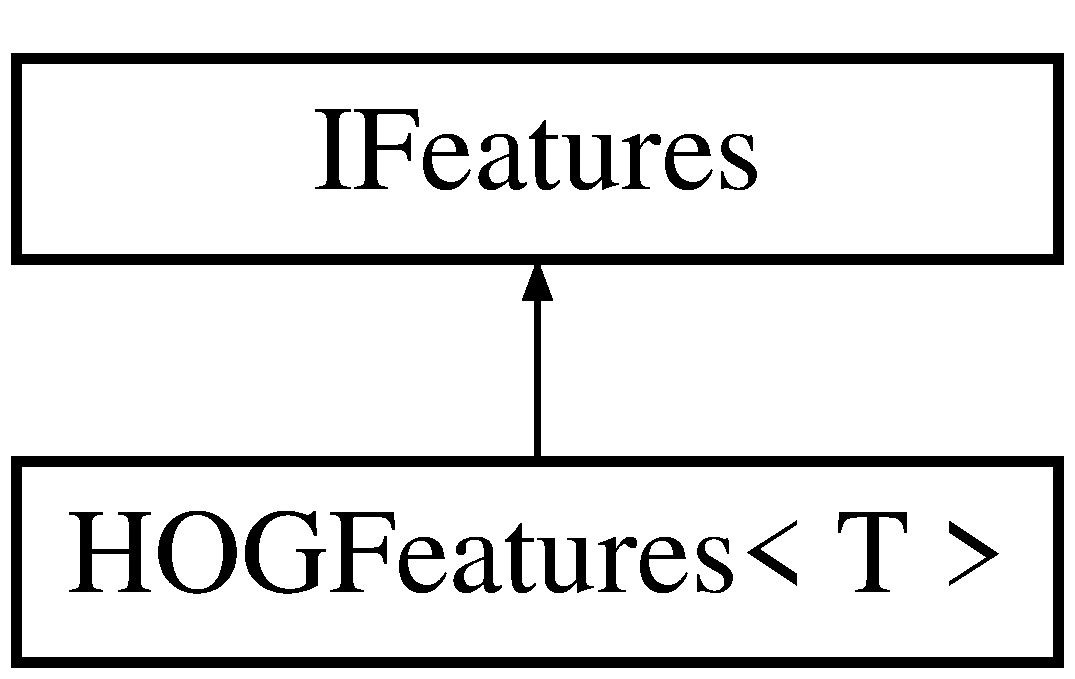
\includegraphics[height=2.000000cm]{class_i_features}
\end{center}
\end{figure}
\subsection*{Public Member Functions}
\begin{DoxyCompactItemize}
\item 
virtual \hyperlink{class_i_features_a7de8c9d6739ebd4504f9d033d71c2f42}{$\sim$\-I\-Features} ()
\item 
virtual size\-\_\-t \hyperlink{class_i_features_a79f6861190d7c2754d560c6c10baa787}{binsize} (void) const =0
\begin{DoxyCompactList}\small\item\em retrieve the spatial binning size (1 if not relevant) \end{DoxyCompactList}\item 
virtual size\-\_\-t \hyperlink{class_i_features_abf8d0bf5f66e7b3188ca73b5c9e48a1f}{nscales} (void) const =0
\begin{DoxyCompactList}\small\item\em retrieve the number of scales the features are calculated over \end{DoxyCompactList}\item 
virtual \hyperlink{types_8hpp_a4da5db3ee9e284f719ef5764dbadffc8}{vectorf} \hyperlink{class_i_features_ad02aea9fd29e438d25e1c7d68c508b9e}{scales} (void) const =0
\begin{DoxyCompactList}\small\item\em the vector of scales \end{DoxyCompactList}\item 
virtual void \hyperlink{class_i_features_a0cd270503671145fae965c8d9fedc91a}{pyramid} (const cv\-::\-Mat \&im, \hyperlink{types_8hpp_a3207a7addcfa415d1c83622febcb1e9b}{vector\-Mat} \&pyrafeatures)=0
\begin{DoxyCompactList}\small\item\em a pyramid of features \end{DoxyCompactList}\end{DoxyCompactItemize}


\subsection{Constructor \& Destructor Documentation}
\hypertarget{class_i_features_a7de8c9d6739ebd4504f9d033d71c2f42}{\index{I\-Features@{I\-Features}!$\sim$\-I\-Features@{$\sim$\-I\-Features}}
\index{$\sim$\-I\-Features@{$\sim$\-I\-Features}!IFeatures@{I\-Features}}
\subsubsection[{$\sim$\-I\-Features}]{\setlength{\rightskip}{0pt plus 5cm}virtual I\-Features\-::$\sim$\-I\-Features (
\begin{DoxyParamCaption}
{}
\end{DoxyParamCaption}
)\hspace{0.3cm}{\ttfamily [inline]}, {\ttfamily [virtual]}}}\label{class_i_features_a7de8c9d6739ebd4504f9d033d71c2f42}


\subsection{Member Function Documentation}
\hypertarget{class_i_features_a79f6861190d7c2754d560c6c10baa787}{\index{I\-Features@{I\-Features}!binsize@{binsize}}
\index{binsize@{binsize}!IFeatures@{I\-Features}}
\subsubsection[{binsize}]{\setlength{\rightskip}{0pt plus 5cm}virtual size\-\_\-t I\-Features\-::binsize (
\begin{DoxyParamCaption}
\item[{void}]{}
\end{DoxyParamCaption}
) const\hspace{0.3cm}{\ttfamily [pure virtual]}}}\label{class_i_features_a79f6861190d7c2754d560c6c10baa787}


retrieve the spatial binning size (1 if not relevant) 



Implemented in \hyperlink{class_h_o_g_features_a0b75015646ceac02ba250e5af86245d4}{H\-O\-G\-Features$<$ T $>$}.

\hypertarget{class_i_features_abf8d0bf5f66e7b3188ca73b5c9e48a1f}{\index{I\-Features@{I\-Features}!nscales@{nscales}}
\index{nscales@{nscales}!IFeatures@{I\-Features}}
\subsubsection[{nscales}]{\setlength{\rightskip}{0pt plus 5cm}virtual size\-\_\-t I\-Features\-::nscales (
\begin{DoxyParamCaption}
\item[{void}]{}
\end{DoxyParamCaption}
) const\hspace{0.3cm}{\ttfamily [pure virtual]}}}\label{class_i_features_abf8d0bf5f66e7b3188ca73b5c9e48a1f}


retrieve the number of scales the features are calculated over 



Implemented in \hyperlink{class_h_o_g_features_a2ea95a95f6d79af3344502b45e1cb7c5}{H\-O\-G\-Features$<$ T $>$}.

\hypertarget{class_i_features_a0cd270503671145fae965c8d9fedc91a}{\index{I\-Features@{I\-Features}!pyramid@{pyramid}}
\index{pyramid@{pyramid}!IFeatures@{I\-Features}}
\subsubsection[{pyramid}]{\setlength{\rightskip}{0pt plus 5cm}virtual void I\-Features\-::pyramid (
\begin{DoxyParamCaption}
\item[{const cv\-::\-Mat \&}]{im, }
\item[{{\bf vector\-Mat} \&}]{pyrafeatures}
\end{DoxyParamCaption}
)\hspace{0.3cm}{\ttfamily [pure virtual]}}}\label{class_i_features_a0cd270503671145fae965c8d9fedc91a}


a pyramid of features 

features calculated of a number of scales 
\begin{DoxyParams}{Parameters}
{\em im} & the input image to calculate features for \\
\hline
{\em pyrafeatures} & an output vector of matrices of features, one matrix for each scale \\
\hline
\end{DoxyParams}


Implemented in \hyperlink{class_h_o_g_features_a509372c4e652c3fc97f2d2be75fecd4d}{H\-O\-G\-Features$<$ T $>$}.

\hypertarget{class_i_features_ad02aea9fd29e438d25e1c7d68c508b9e}{\index{I\-Features@{I\-Features}!scales@{scales}}
\index{scales@{scales}!IFeatures@{I\-Features}}
\subsubsection[{scales}]{\setlength{\rightskip}{0pt plus 5cm}virtual {\bf vectorf} I\-Features\-::scales (
\begin{DoxyParamCaption}
\item[{void}]{}
\end{DoxyParamCaption}
) const\hspace{0.3cm}{\ttfamily [pure virtual]}}}\label{class_i_features_ad02aea9fd29e438d25e1c7d68c508b9e}


the vector of scales 

the vector of scales, 1 indicating the native image resolution, values lower than 1 indicating downsampled images, and values greater than 1 indicating hallucinated resolutions 

Implemented in \hyperlink{class_h_o_g_features_ad9668fda860881c676e1d1bd70adc18c}{H\-O\-G\-Features$<$ T $>$}.



The documentation for this class was generated from the following file\-:\begin{DoxyCompactItemize}
\item 
/\-Users/m29474/\-Desktop/code/openbr/3rdparty/\-Parts\-Based\-Detector/include/\hyperlink{_i_features_8hpp}{I\-Features.\-hpp}\end{DoxyCompactItemize}

\hypertarget{class_math}{\section{Math Class Reference}
\label{class_math}\index{Math@{Math}}
}


{\ttfamily \#include $<$Math.\-hpp$>$}

\subsection*{Public Member Functions}
\begin{DoxyCompactItemize}
\item 
virtual \hyperlink{class_math_a28ea971a536094b9083ec8f36ff357e5}{$\sim$\-Math} ()
\end{DoxyCompactItemize}
\subsection*{Static Public Member Functions}
\begin{DoxyCompactItemize}
\item 
{\footnotesize template$<$typename T $>$ }\\static T \hyperlink{class_math_aca890c10f12205897ac47792494d149f}{median} (const cv\-::\-Mat \&mat)
\begin{DoxyCompactList}\small\item\em return the median value of a matrix \end{DoxyCompactList}\item 
static void \hyperlink{class_math_a08953b39d9d278ee0bb2a15bda7fd1a2}{find} (const cv\-::\-Mat \&binary, std\-::vector$<$ cv\-::\-Point $>$ \&idx)
\begin{DoxyCompactList}\small\item\em find nonzero elements in a matrix \end{DoxyCompactList}\item 
{\footnotesize template$<$typename T $>$ }\\static void \hyperlink{class_math_a1c558fca5013d16a9df3adf2caa7c610}{reduce\-Pick\-Index} (const \hyperlink{types_8hpp_a3207a7addcfa415d1c83622febcb1e9b}{vector\-Mat} \&in, const cv\-::\-Mat \&idx, cv\-::\-Mat \&out)
\begin{DoxyCompactList}\small\item\em Reduce a vector of matrices via indexing. \end{DoxyCompactList}\item 
{\footnotesize template$<$typename T $>$ }\\static void \hyperlink{class_math_a97f8ffb7a7855e6cc0dabcef0817bafa}{reduce\-Max} (const \hyperlink{types_8hpp_a3207a7addcfa415d1c83622febcb1e9b}{vector\-Mat} \&in, cv\-::\-Mat \&maxv, cv\-::\-Mat \&maxi)
\begin{DoxyCompactList}\small\item\em Reduce a vector of matrices via elementwise max. \end{DoxyCompactList}\end{DoxyCompactItemize}
\subsection*{Private Member Functions}
\begin{DoxyCompactItemize}
\item 
\hyperlink{class_math_a4b0f0a2da150d3fbfdb71524420c9fbf}{Math} ()
\end{DoxyCompactItemize}


\subsection{Constructor \& Destructor Documentation}
\hypertarget{class_math_a4b0f0a2da150d3fbfdb71524420c9fbf}{\index{Math@{Math}!Math@{Math}}
\index{Math@{Math}!Math@{Math}}
\subsubsection[{Math}]{\setlength{\rightskip}{0pt plus 5cm}Math\-::\-Math (
\begin{DoxyParamCaption}
{}
\end{DoxyParamCaption}
)\hspace{0.3cm}{\ttfamily [inline]}, {\ttfamily [private]}}}\label{class_math_a4b0f0a2da150d3fbfdb71524420c9fbf}
\hypertarget{class_math_a28ea971a536094b9083ec8f36ff357e5}{\index{Math@{Math}!$\sim$\-Math@{$\sim$\-Math}}
\index{$\sim$\-Math@{$\sim$\-Math}!Math@{Math}}
\subsubsection[{$\sim$\-Math}]{\setlength{\rightskip}{0pt plus 5cm}virtual Math\-::$\sim$\-Math (
\begin{DoxyParamCaption}
{}
\end{DoxyParamCaption}
)\hspace{0.3cm}{\ttfamily [inline]}, {\ttfamily [virtual]}}}\label{class_math_a28ea971a536094b9083ec8f36ff357e5}


\subsection{Member Function Documentation}
\hypertarget{class_math_a08953b39d9d278ee0bb2a15bda7fd1a2}{\index{Math@{Math}!find@{find}}
\index{find@{find}!Math@{Math}}
\subsubsection[{find}]{\setlength{\rightskip}{0pt plus 5cm}static void Math\-::find (
\begin{DoxyParamCaption}
\item[{const cv\-::\-Mat \&}]{binary, }
\item[{std\-::vector$<$ cv\-::\-Point $>$ \&}]{idx}
\end{DoxyParamCaption}
)\hspace{0.3cm}{\ttfamily [inline]}, {\ttfamily [static]}}}\label{class_math_a08953b39d9d278ee0bb2a15bda7fd1a2}


find nonzero elements in a matrix 

Find all nonzero elements in a matrix of type C\-V\-\_\-8\-U, and return the indieces (x,y) of the nonzero pixels in an array of Point


\begin{DoxyParams}{Parameters}
{\em binary} & the input image (usually the output of a comparison operation such as compare(), $>$, ==, etc) \\
\hline
{\em idx} & the output vector of nonzero indices \\
\hline
\end{DoxyParams}
\hypertarget{class_math_aca890c10f12205897ac47792494d149f}{\index{Math@{Math}!median@{median}}
\index{median@{median}!Math@{Math}}
\subsubsection[{median}]{\setlength{\rightskip}{0pt plus 5cm}template$<$typename T $>$ static T Math\-::median (
\begin{DoxyParamCaption}
\item[{const cv\-::\-Mat \&}]{mat}
\end{DoxyParamCaption}
)\hspace{0.3cm}{\ttfamily [inline]}, {\ttfamily [static]}}}\label{class_math_aca890c10f12205897ac47792494d149f}


return the median value of a matrix 


\begin{DoxyParams}{Parameters}
{\em mat} & the input matrix \\
\hline
\end{DoxyParams}
\begin{DoxyReturn}{Returns}
the median value, of the same precision as the input 
\end{DoxyReturn}
\hypertarget{class_math_a97f8ffb7a7855e6cc0dabcef0817bafa}{\index{Math@{Math}!reduce\-Max@{reduce\-Max}}
\index{reduce\-Max@{reduce\-Max}!Math@{Math}}
\subsubsection[{reduce\-Max}]{\setlength{\rightskip}{0pt plus 5cm}template$<$typename T $>$ static void Math\-::reduce\-Max (
\begin{DoxyParamCaption}
\item[{const {\bf vector\-Mat} \&}]{in, }
\item[{cv\-::\-Mat \&}]{maxv, }
\item[{cv\-::\-Mat \&}]{maxi}
\end{DoxyParamCaption}
)\hspace{0.3cm}{\ttfamily [inline]}, {\ttfamily [static]}}}\label{class_math_a97f8ffb7a7855e6cc0dabcef0817bafa}


Reduce a vector of matrices via elementwise max. 

Reduce a 3\-D matrix (represented as a vector of matrices using cv\-::split() ) to a 2\-D matrix by taking the elementwise maximum across the 3\-D dimension. Therefore in.\-size() == out.\-size() \&\& out.\-channels() == 1


\begin{DoxyParams}{Parameters}
{\em in} & the input 3\-D matrix \\
\hline
{\em maxv} & the output 2\-D matrix, containing the maximal values \\
\hline
{\em maxi} & the output 2\-D matrix, containing the maximal indices \\
\hline
\end{DoxyParams}
\hypertarget{class_math_a1c558fca5013d16a9df3adf2caa7c610}{\index{Math@{Math}!reduce\-Pick\-Index@{reduce\-Pick\-Index}}
\index{reduce\-Pick\-Index@{reduce\-Pick\-Index}!Math@{Math}}
\subsubsection[{reduce\-Pick\-Index}]{\setlength{\rightskip}{0pt plus 5cm}template$<$typename T $>$ static void Math\-::reduce\-Pick\-Index (
\begin{DoxyParamCaption}
\item[{const {\bf vector\-Mat} \&}]{in, }
\item[{const cv\-::\-Mat \&}]{idx, }
\item[{cv\-::\-Mat \&}]{out}
\end{DoxyParamCaption}
)\hspace{0.3cm}{\ttfamily [inline]}, {\ttfamily [static]}}}\label{class_math_a1c558fca5013d16a9df3adf2caa7c610}


Reduce a vector of matrices via indexing. 

Reduce a 3\-D matrix (represented as a vector of matrices using cv\-::split() ) to a 2\-D matrix by choosing a single element from each ray cast through the third dimension. This loosely emulates Matlab's matrix indexing functionality

out\mbox{[}i\mbox{]}\mbox{[}j\mbox{]} == in\mbox{[}i\mbox{]}\mbox{[}j\mbox{]}\mbox{[} idx\mbox{[}i\mbox{]}\mbox{[}j\mbox{]} \mbox{]}, forall i,j


\begin{DoxyParams}{Parameters}
{\em in} & the input 3\-D matrix \\
\hline
{\em idx} & the index to choose at each element (idx.\-size() == in\mbox{[}k\mbox{]}.size() forall k) \\
\hline
{\em out} & the flatten 2\-D output matrix \\
\hline
\end{DoxyParams}


The documentation for this class was generated from the following file\-:\begin{DoxyCompactItemize}
\item 
/\-Users/m29474/\-Desktop/code/openbr/3rdparty/\-Parts\-Based\-Detector/include/\hyperlink{_math_8hpp}{Math.\-hpp}\end{DoxyCompactItemize}

\hypertarget{class_matlab_i_o_model}{\section{Matlab\-I\-O\-Model Class Reference}
\label{class_matlab_i_o_model}\index{Matlab\-I\-O\-Model@{Matlab\-I\-O\-Model}}
}


\hyperlink{class_model}{Model} implementation with Matlab .Mat file deserialization.  




{\ttfamily \#include $<$Matlab\-I\-O\-Model.\-hpp$>$}

Inheritance diagram for Matlab\-I\-O\-Model\-:\begin{figure}[H]
\begin{center}
\leavevmode
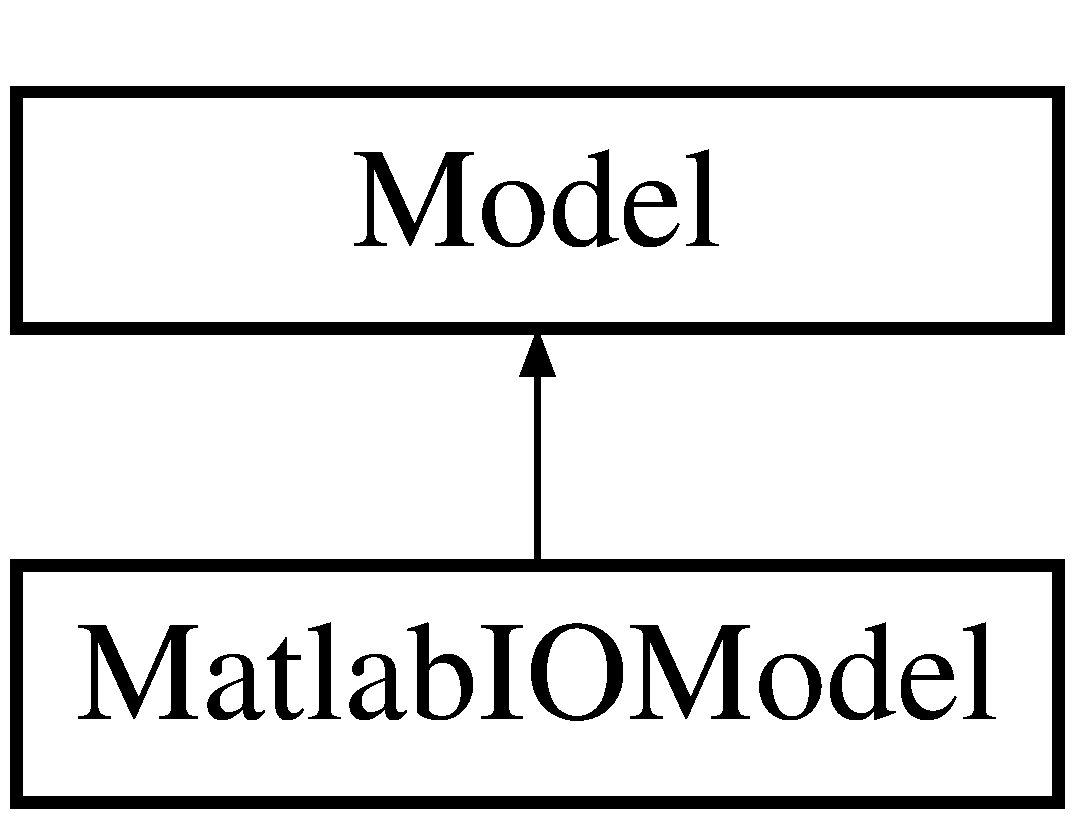
\includegraphics[height=2.000000cm]{class_matlab_i_o_model}
\end{center}
\end{figure}
\subsection*{Public Member Functions}
\begin{DoxyCompactItemize}
\item 
\hyperlink{class_matlab_i_o_model_ac4e387c6665a094f985b0ca0c37b1aee}{Matlab\-I\-O\-Model} ()
\item 
virtual \hyperlink{class_matlab_i_o_model_ac47ddec68b26241297c266b248c856d6}{$\sim$\-Matlab\-I\-O\-Model} ()
\item 
bool \hyperlink{class_matlab_i_o_model_a223538821bf7944a26433f7f99017f8b}{deserialize} (const std\-::string \&filename)
\begin{DoxyCompactList}\small\item\em deserialize a Matlab .Mat file into memory \end{DoxyCompactList}\item 
bool \hyperlink{class_matlab_i_o_model_ad67a1237af4a4e4d736599e6f2474252}{serialize} (const std\-::string \&filename) const 
\end{DoxyCompactItemize}
\subsection*{Additional Inherited Members}


\subsection{Detailed Description}
\hyperlink{class_model}{Model} implementation with Matlab .Mat file deserialization. 

\subsection{Constructor \& Destructor Documentation}
\hypertarget{class_matlab_i_o_model_ac4e387c6665a094f985b0ca0c37b1aee}{\index{Matlab\-I\-O\-Model@{Matlab\-I\-O\-Model}!Matlab\-I\-O\-Model@{Matlab\-I\-O\-Model}}
\index{Matlab\-I\-O\-Model@{Matlab\-I\-O\-Model}!MatlabIOModel@{Matlab\-I\-O\-Model}}
\subsubsection[{Matlab\-I\-O\-Model}]{\setlength{\rightskip}{0pt plus 5cm}Matlab\-I\-O\-Model\-::\-Matlab\-I\-O\-Model (
\begin{DoxyParamCaption}
{}
\end{DoxyParamCaption}
)\hspace{0.3cm}{\ttfamily [inline]}}}\label{class_matlab_i_o_model_ac4e387c6665a094f985b0ca0c37b1aee}
\hypertarget{class_matlab_i_o_model_ac47ddec68b26241297c266b248c856d6}{\index{Matlab\-I\-O\-Model@{Matlab\-I\-O\-Model}!$\sim$\-Matlab\-I\-O\-Model@{$\sim$\-Matlab\-I\-O\-Model}}
\index{$\sim$\-Matlab\-I\-O\-Model@{$\sim$\-Matlab\-I\-O\-Model}!MatlabIOModel@{Matlab\-I\-O\-Model}}
\subsubsection[{$\sim$\-Matlab\-I\-O\-Model}]{\setlength{\rightskip}{0pt plus 5cm}virtual Matlab\-I\-O\-Model\-::$\sim$\-Matlab\-I\-O\-Model (
\begin{DoxyParamCaption}
{}
\end{DoxyParamCaption}
)\hspace{0.3cm}{\ttfamily [inline]}, {\ttfamily [virtual]}}}\label{class_matlab_i_o_model_ac47ddec68b26241297c266b248c856d6}


\subsection{Member Function Documentation}
\hypertarget{class_matlab_i_o_model_a223538821bf7944a26433f7f99017f8b}{\index{Matlab\-I\-O\-Model@{Matlab\-I\-O\-Model}!deserialize@{deserialize}}
\index{deserialize@{deserialize}!MatlabIOModel@{Matlab\-I\-O\-Model}}
\subsubsection[{deserialize}]{\setlength{\rightskip}{0pt plus 5cm}bool Matlab\-I\-O\-Model\-::deserialize (
\begin{DoxyParamCaption}
\item[{const std\-::string \&}]{filename}
\end{DoxyParamCaption}
)\hspace{0.3cm}{\ttfamily [virtual]}}}\label{class_matlab_i_o_model_a223538821bf7944a26433f7f99017f8b}


deserialize a Matlab .Mat file into memory 

deserialize a valid version 5 .Mat file using the underlying Matlab\-I\-O parser, and populate the model fields. If any of the fields do not exist, or a bad type cast is attempted, an exception will be thrown


\begin{DoxyParams}{Parameters}
{\em filename} & the path to the model file \\
\hline
\end{DoxyParams}
\begin{DoxyReturn}{Returns}
true if the file was found, opened and verified to be a valid Matlab version 5 file 
\end{DoxyReturn}

\begin{DoxyExceptions}{Exceptions}
{\em boost\-::bad\-\_\-any\-\_\-cast,exception} & \\
\hline
\end{DoxyExceptions}


Implements \hyperlink{class_model_a2fc5d668c4930e8172e1a1460a8e6b46}{Model}.

\hypertarget{class_matlab_i_o_model_ad67a1237af4a4e4d736599e6f2474252}{\index{Matlab\-I\-O\-Model@{Matlab\-I\-O\-Model}!serialize@{serialize}}
\index{serialize@{serialize}!MatlabIOModel@{Matlab\-I\-O\-Model}}
\subsubsection[{serialize}]{\setlength{\rightskip}{0pt plus 5cm}bool Matlab\-I\-O\-Model\-::serialize (
\begin{DoxyParamCaption}
\item[{const std\-::string \&}]{filename}
\end{DoxyParamCaption}
) const\hspace{0.3cm}{\ttfamily [virtual]}}}\label{class_matlab_i_o_model_ad67a1237af4a4e4d736599e6f2474252}


Implements \hyperlink{class_model_a952f21d72d87aa30387ea6e5c1d603fd}{Model}.



The documentation for this class was generated from the following files\-:\begin{DoxyCompactItemize}
\item 
/\-Users/m29474/\-Desktop/code/openbr/3rdparty/\-Parts\-Based\-Detector/include/\hyperlink{_matlab_i_o_model_8hpp}{Matlab\-I\-O\-Model.\-hpp}\item 
/\-Users/m29474/\-Desktop/code/openbr/3rdparty/\-Parts\-Based\-Detector/src/\hyperlink{_matlab_i_o_model_8cpp}{Matlab\-I\-O\-Model.\-cpp}\end{DoxyCompactItemize}

\hypertarget{class_metrics}{\section{Metrics Class Reference}
\label{class_metrics}\index{Metrics@{Metrics}}
}


{\ttfamily \#include $<$Metrics.\-hpp$>$}

\subsection*{Private Attributes}
\begin{DoxyCompactItemize}
\item 
cv\-::\-Mat \hyperlink{class_metrics_aba72e7e31eb9057d1252e61cdf3aa904}{camera\-\_\-matrix}
\end{DoxyCompactItemize}


\subsection{Field Documentation}
\hypertarget{class_metrics_aba72e7e31eb9057d1252e61cdf3aa904}{\index{Metrics@{Metrics}!camera\-\_\-matrix@{camera\-\_\-matrix}}
\index{camera\-\_\-matrix@{camera\-\_\-matrix}!Metrics@{Metrics}}
\subsubsection[{camera\-\_\-matrix}]{\setlength{\rightskip}{0pt plus 5cm}cv\-::\-Mat Metrics\-::camera\-\_\-matrix\hspace{0.3cm}{\ttfamily [private]}}}\label{class_metrics_aba72e7e31eb9057d1252e61cdf3aa904}


The documentation for this class was generated from the following file\-:\begin{DoxyCompactItemize}
\item 
/\-Users/m29474/\-Desktop/code/openbr/3rdparty/\-Parts\-Based\-Detector/include/\hyperlink{_metrics_8hpp}{Metrics.\-hpp}\end{DoxyCompactItemize}

\hypertarget{class_model}{\section{Model Class Reference}
\label{class_model}\index{Model@{Model}}
}


Monolithic container class for storing model parameters.  




{\ttfamily \#include $<$Model.\-hpp$>$}

Inheritance diagram for Model\-:\begin{figure}[H]
\begin{center}
\leavevmode
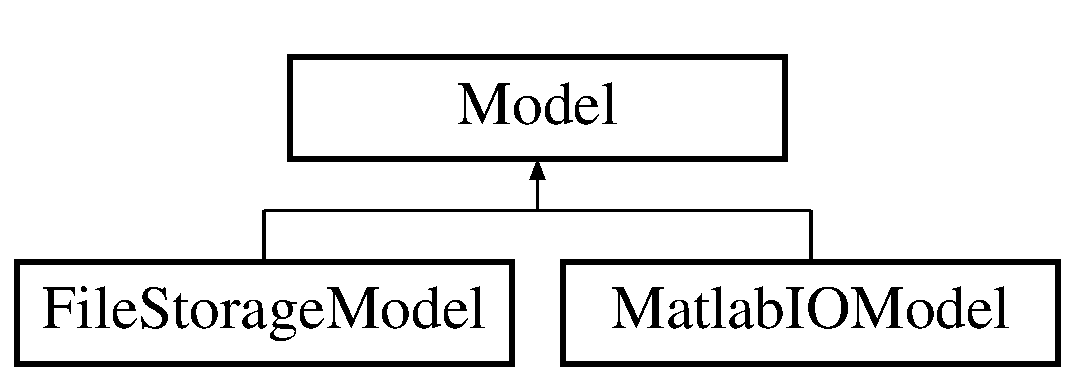
\includegraphics[height=2.000000cm]{class_model}
\end{center}
\end{figure}
\subsection*{Public Member Functions}
\begin{DoxyCompactItemize}
\item 
\hyperlink{class_model_ae3b375de5f6df4faf74a95d64748e048}{Model} ()
\item 
virtual \hyperlink{class_model_af032d8433c87a0a3a431faf6563a1f03}{$\sim$\-Model} ()
\item 
\hyperlink{types_8hpp_a3207a7addcfa415d1c83622febcb1e9b}{vector\-Mat} \& \hyperlink{class_model_ad923232199aa30bb69436fd08ef01b6d}{filters} (void)
\item 
\hyperlink{types_8hpp_a44529587d60e73bf0e689a82e5e70a55}{vectori} \& \hyperlink{class_model_a66a09e10ef051d4c261546d4016b7d74}{filtersi} (void)
\item 
\hyperlink{types_8hpp_a94f2d563f3725231a6f684b4dce4f1ef}{vector2\-Df} \& \hyperlink{class_model_a2d471c6cb6ab4273963b986e21f91f82}{def} (void)
\item 
\hyperlink{types_8hpp_a44529587d60e73bf0e689a82e5e70a55}{vectori} \& \hyperlink{class_model_a68d158f45c15ca0417b97cc140c498c6}{defi} (void)
\item 
\hyperlink{types_8hpp_a4da5db3ee9e284f719ef5764dbadffc8}{vectorf} \& \hyperlink{class_model_aad5223ba9a48a9d4301d004d11457006}{bias} (void)
\item 
\hyperlink{types_8hpp_a44529587d60e73bf0e689a82e5e70a55}{vectori} \& \hyperlink{class_model_a478f9460cf39e00f0d65c0afbecd8677}{biasi} (void)
\item 
\hyperlink{types_8hpp_ac468fcf6870d6563ac8fa3669845afcc}{vector\-Point} \& \hyperlink{class_model_a047262c3a9de203b9d67094128c483a5}{anchors} (void)
\item 
\hyperlink{types_8hpp_a1f7c8ad00a53fb2d61b3656da9a6581d}{vector3\-Di} \& \hyperlink{class_model_a35c8491baa7893180abf62f22be40499}{filterid} (void)
\item 
\hyperlink{types_8hpp_a1f7c8ad00a53fb2d61b3656da9a6581d}{vector3\-Di} \& \hyperlink{class_model_a4088cf71d411e0cbbef2eb7c0861b039}{biasid} (void)
\item 
\hyperlink{types_8hpp_a1f7c8ad00a53fb2d61b3656da9a6581d}{vector3\-Di} \& \hyperlink{class_model_a2efd0f976fb014b3267281fd79172921}{defid} (void)
\item 
\hyperlink{types_8hpp_a93a5e2cfd40d1ff1f10d8bbf11884c41}{vector2\-Di} \& \hyperlink{class_model_a2a44477641549a9c8ebecfff9221bda9}{parentid} (void)
\item 
std\-::string \hyperlink{class_model_aeae6527ff13db7724c53c942029d882d}{name} (void)
\item 
\hyperlink{types_8hpp_a44529587d60e73bf0e689a82e5e70a55}{vectori} \& \hyperlink{class_model_a65d5e15900bc329b42acc7ce57c45628}{conn} (void)
\item 
int \hyperlink{class_model_aadbe1db9da272e3c7925f14c10143360}{nparts} (void) const 
\item 
int \hyperlink{class_model_a86676b7fdc842393897b11ce8a7d7623}{nmixtures} (void) const 
\item 
float \hyperlink{class_model_a474739b5b87ebfc7342d10124dfd59b6}{thresh} (void) const 
\item 
int \hyperlink{class_model_a93d5e6030b6ea9ffe155b459d9e58585}{binsize} (void) const 
\item 
int \hyperlink{class_model_a3de9632d7c459c2d7ea961be84005921}{nscales} (void) const 
\item 
int \hyperlink{class_model_ad9ff4f0d1dd752dd96f6ff4a47e3486d}{flen} (void) const 
\item 
int \hyperlink{class_model_ab64488cd01aa451323bf1e30603fbc73}{norient} (void) const 
\item 
int \hyperlink{class_model_acaee5d575cfdb39a4a6ebc3b765a88bc}{ncomponents} (void) const 
\item 
virtual bool \hyperlink{class_model_a952f21d72d87aa30387ea6e5c1d603fd}{serialize} (const std\-::string \&filename) const =0
\item 
virtual bool \hyperlink{class_model_a2fc5d668c4930e8172e1a1460a8e6b46}{deserialize} (const std\-::string \&filename)=0
\end{DoxyCompactItemize}
\subsection*{Protected Attributes}
\begin{DoxyCompactItemize}
\item 
\hyperlink{types_8hpp_a3207a7addcfa415d1c83622febcb1e9b}{vector\-Mat} \hyperlink{class_model_ac8594fac5ef6d874cf0a4f2fd856914d}{filtersw\-\_\-}
\begin{DoxyCompactList}\small\item\em the filter weights \end{DoxyCompactList}\item 
\hyperlink{types_8hpp_a44529587d60e73bf0e689a82e5e70a55}{vectori} \hyperlink{class_model_ab3f13d90cc96c70d4b454db12528f85f}{filtersi\-\_\-}
\begin{DoxyCompactList}\small\item\em the filer indices \end{DoxyCompactList}\item 
\hyperlink{types_8hpp_a94f2d563f3725231a6f684b4dce4f1ef}{vector2\-Df} \hyperlink{class_model_a1e1fba557437a9f4c0ef1535a64d83f2}{defw\-\_\-}
\begin{DoxyCompactList}\small\item\em the deformation weights \end{DoxyCompactList}\item 
\hyperlink{types_8hpp_a44529587d60e73bf0e689a82e5e70a55}{vectori} \hyperlink{class_model_a477df0e7641f38782085d0a425625d12}{defi\-\_\-}
\begin{DoxyCompactList}\small\item\em the deformation indices \end{DoxyCompactList}\item 
\hyperlink{types_8hpp_a4da5db3ee9e284f719ef5764dbadffc8}{vectorf} \hyperlink{class_model_ab870c45d7637a43ba73c81cc4080a497}{biasw\-\_\-}
\begin{DoxyCompactList}\small\item\em the bias weights \end{DoxyCompactList}\item 
\hyperlink{types_8hpp_a44529587d60e73bf0e689a82e5e70a55}{vectori} \hyperlink{class_model_a0306acb4cfa28b6f13ccd76c011d20ac}{biasi\-\_\-}
\begin{DoxyCompactList}\small\item\em the bias indices \end{DoxyCompactList}\item 
\hyperlink{types_8hpp_ac468fcf6870d6563ac8fa3669845afcc}{vector\-Point} \hyperlink{class_model_ac2aa3eb0450ac05d0a3c7274b4ad91eb}{anchors\-\_\-}
\begin{DoxyCompactList}\small\item\em the anchors (part position relative to parent) \end{DoxyCompactList}\item 
\hyperlink{types_8hpp_a1f7c8ad00a53fb2d61b3656da9a6581d}{vector3\-Di} \hyperlink{class_model_a7c3905dd5e45a2e60da02c783a49db9c}{biasid\-\_\-}
\begin{DoxyCompactList}\small\item\em indexing schema for the bias (weights and indices) \end{DoxyCompactList}\item 
\hyperlink{types_8hpp_a1f7c8ad00a53fb2d61b3656da9a6581d}{vector3\-Di} \hyperlink{class_model_a08e65111230ab010535cc9485dfd6d0d}{filterid\-\_\-}
\begin{DoxyCompactList}\small\item\em indexing schema for the filters (weights and indices) \end{DoxyCompactList}\item 
\hyperlink{types_8hpp_a1f7c8ad00a53fb2d61b3656da9a6581d}{vector3\-Di} \hyperlink{class_model_a381f13c9035313ffd1cb67e07a2e84bd}{defid\-\_\-}
\begin{DoxyCompactList}\small\item\em indexing schema for the deformation (weights, indices and anchors \end{DoxyCompactList}\item 
\hyperlink{types_8hpp_a93a5e2cfd40d1ff1f10d8bbf11884c41}{vector2\-Di} \hyperlink{class_model_a4e1151fe7911f52ec75944eff1b257f4}{parentid\-\_\-}
\begin{DoxyCompactList}\small\item\em indexing schema for the parent (for biasid\-\_\-, filterid\-\_\- and defid\-\_\-) \end{DoxyCompactList}\item 
std\-::string \hyperlink{class_model_afca3bde5ad33e936c455d3d311b8406d}{name\-\_\-}
\begin{DoxyCompactList}\small\item\em a unique string identifier for the model \end{DoxyCompactList}\item 
\hyperlink{types_8hpp_a44529587d60e73bf0e689a82e5e70a55}{vectori} \hyperlink{class_model_a976b10b7048b41203eae19c141654abf}{conn\-\_\-}
\begin{DoxyCompactList}\small\item\em the connectivity of the parts, where each element is a reference to the part's parent \end{DoxyCompactList}\item 
int \hyperlink{class_model_ae8b3d33dbc43d6ab07c1553c9a1bbc2e}{nparts\-\_\-}
\begin{DoxyCompactList}\small\item\em the number of parts \end{DoxyCompactList}\item 
int \hyperlink{class_model_a047a8d7591bde166f0c3ab36a2130b53}{nmixtures\-\_\-}
\begin{DoxyCompactList}\small\item\em the number of mixtures \end{DoxyCompactList}\item 
int \hyperlink{class_model_ab711641b36aa9b8b578acf151af55aa7}{nscales\-\_\-}
\begin{DoxyCompactList}\small\item\em the number of scales at which to compute features \end{DoxyCompactList}\item 
float \hyperlink{class_model_ac2263c14bbd27a5fed433494354e2b02}{thresh\-\_\-}
\begin{DoxyCompactList}\small\item\em the threshold for a positive detection \end{DoxyCompactList}\item 
int \hyperlink{class_model_af34c4284d739cac02812d76eaa231679}{binsize\-\_\-}
\begin{DoxyCompactList}\small\item\em the spatial pooling size when computing features \end{DoxyCompactList}\item 
int \hyperlink{class_model_afafec86aa7175a4664ae76d545f084ea}{flen\-\_\-}
\begin{DoxyCompactList}\small\item\em the length of the feature vector in each bin \end{DoxyCompactList}\item 
int \hyperlink{class_model_a40c5597450f8efb960bb7da74890e73c}{norient\-\_\-}
\begin{DoxyCompactList}\small\item\em the number of orientations per H\-O\-G feature bin \end{DoxyCompactList}\end{DoxyCompactItemize}


\subsection{Detailed Description}
Monolithic container class for storing model parameters. 

\subsection{Constructor \& Destructor Documentation}
\hypertarget{class_model_ae3b375de5f6df4faf74a95d64748e048}{\index{Model@{Model}!Model@{Model}}
\index{Model@{Model}!Model@{Model}}
\subsubsection[{Model}]{\setlength{\rightskip}{0pt plus 5cm}Model\-::\-Model (
\begin{DoxyParamCaption}
{}
\end{DoxyParamCaption}
)\hspace{0.3cm}{\ttfamily [inline]}}}\label{class_model_ae3b375de5f6df4faf74a95d64748e048}
\hypertarget{class_model_af032d8433c87a0a3a431faf6563a1f03}{\index{Model@{Model}!$\sim$\-Model@{$\sim$\-Model}}
\index{$\sim$\-Model@{$\sim$\-Model}!Model@{Model}}
\subsubsection[{$\sim$\-Model}]{\setlength{\rightskip}{0pt plus 5cm}virtual Model\-::$\sim$\-Model (
\begin{DoxyParamCaption}
{}
\end{DoxyParamCaption}
)\hspace{0.3cm}{\ttfamily [inline]}, {\ttfamily [virtual]}}}\label{class_model_af032d8433c87a0a3a431faf6563a1f03}


\subsection{Member Function Documentation}
\hypertarget{class_model_a047262c3a9de203b9d67094128c483a5}{\index{Model@{Model}!anchors@{anchors}}
\index{anchors@{anchors}!Model@{Model}}
\subsubsection[{anchors}]{\setlength{\rightskip}{0pt plus 5cm}{\bf vector\-Point}\& Model\-::anchors (
\begin{DoxyParamCaption}
\item[{void}]{}
\end{DoxyParamCaption}
)\hspace{0.3cm}{\ttfamily [inline]}}}\label{class_model_a047262c3a9de203b9d67094128c483a5}
\hypertarget{class_model_aad5223ba9a48a9d4301d004d11457006}{\index{Model@{Model}!bias@{bias}}
\index{bias@{bias}!Model@{Model}}
\subsubsection[{bias}]{\setlength{\rightskip}{0pt plus 5cm}{\bf vectorf}\& Model\-::bias (
\begin{DoxyParamCaption}
\item[{void}]{}
\end{DoxyParamCaption}
)\hspace{0.3cm}{\ttfamily [inline]}}}\label{class_model_aad5223ba9a48a9d4301d004d11457006}
\hypertarget{class_model_a478f9460cf39e00f0d65c0afbecd8677}{\index{Model@{Model}!biasi@{biasi}}
\index{biasi@{biasi}!Model@{Model}}
\subsubsection[{biasi}]{\setlength{\rightskip}{0pt plus 5cm}{\bf vectori}\& Model\-::biasi (
\begin{DoxyParamCaption}
\item[{void}]{}
\end{DoxyParamCaption}
)\hspace{0.3cm}{\ttfamily [inline]}}}\label{class_model_a478f9460cf39e00f0d65c0afbecd8677}
\hypertarget{class_model_a4088cf71d411e0cbbef2eb7c0861b039}{\index{Model@{Model}!biasid@{biasid}}
\index{biasid@{biasid}!Model@{Model}}
\subsubsection[{biasid}]{\setlength{\rightskip}{0pt plus 5cm}{\bf vector3\-Di}\& Model\-::biasid (
\begin{DoxyParamCaption}
\item[{void}]{}
\end{DoxyParamCaption}
)\hspace{0.3cm}{\ttfamily [inline]}}}\label{class_model_a4088cf71d411e0cbbef2eb7c0861b039}
\hypertarget{class_model_a93d5e6030b6ea9ffe155b459d9e58585}{\index{Model@{Model}!binsize@{binsize}}
\index{binsize@{binsize}!Model@{Model}}
\subsubsection[{binsize}]{\setlength{\rightskip}{0pt plus 5cm}int Model\-::binsize (
\begin{DoxyParamCaption}
\item[{void}]{}
\end{DoxyParamCaption}
) const\hspace{0.3cm}{\ttfamily [inline]}}}\label{class_model_a93d5e6030b6ea9ffe155b459d9e58585}
\hypertarget{class_model_a65d5e15900bc329b42acc7ce57c45628}{\index{Model@{Model}!conn@{conn}}
\index{conn@{conn}!Model@{Model}}
\subsubsection[{conn}]{\setlength{\rightskip}{0pt plus 5cm}{\bf vectori}\& Model\-::conn (
\begin{DoxyParamCaption}
\item[{void}]{}
\end{DoxyParamCaption}
)\hspace{0.3cm}{\ttfamily [inline]}}}\label{class_model_a65d5e15900bc329b42acc7ce57c45628}
\hypertarget{class_model_a2d471c6cb6ab4273963b986e21f91f82}{\index{Model@{Model}!def@{def}}
\index{def@{def}!Model@{Model}}
\subsubsection[{def}]{\setlength{\rightskip}{0pt plus 5cm}{\bf vector2\-Df}\& Model\-::def (
\begin{DoxyParamCaption}
\item[{void}]{}
\end{DoxyParamCaption}
)\hspace{0.3cm}{\ttfamily [inline]}}}\label{class_model_a2d471c6cb6ab4273963b986e21f91f82}
\hypertarget{class_model_a68d158f45c15ca0417b97cc140c498c6}{\index{Model@{Model}!defi@{defi}}
\index{defi@{defi}!Model@{Model}}
\subsubsection[{defi}]{\setlength{\rightskip}{0pt plus 5cm}{\bf vectori}\& Model\-::defi (
\begin{DoxyParamCaption}
\item[{void}]{}
\end{DoxyParamCaption}
)\hspace{0.3cm}{\ttfamily [inline]}}}\label{class_model_a68d158f45c15ca0417b97cc140c498c6}
\hypertarget{class_model_a2efd0f976fb014b3267281fd79172921}{\index{Model@{Model}!defid@{defid}}
\index{defid@{defid}!Model@{Model}}
\subsubsection[{defid}]{\setlength{\rightskip}{0pt plus 5cm}{\bf vector3\-Di}\& Model\-::defid (
\begin{DoxyParamCaption}
\item[{void}]{}
\end{DoxyParamCaption}
)\hspace{0.3cm}{\ttfamily [inline]}}}\label{class_model_a2efd0f976fb014b3267281fd79172921}
\hypertarget{class_model_a2fc5d668c4930e8172e1a1460a8e6b46}{\index{Model@{Model}!deserialize@{deserialize}}
\index{deserialize@{deserialize}!Model@{Model}}
\subsubsection[{deserialize}]{\setlength{\rightskip}{0pt plus 5cm}virtual bool Model\-::deserialize (
\begin{DoxyParamCaption}
\item[{const std\-::string \&}]{filename}
\end{DoxyParamCaption}
)\hspace{0.3cm}{\ttfamily [pure virtual]}}}\label{class_model_a2fc5d668c4930e8172e1a1460a8e6b46}


Implemented in \hyperlink{class_file_storage_model_af97e8cf0ced06893ffca6ec119a31143}{File\-Storage\-Model}, and \hyperlink{class_matlab_i_o_model_a223538821bf7944a26433f7f99017f8b}{Matlab\-I\-O\-Model}.

\hypertarget{class_model_a35c8491baa7893180abf62f22be40499}{\index{Model@{Model}!filterid@{filterid}}
\index{filterid@{filterid}!Model@{Model}}
\subsubsection[{filterid}]{\setlength{\rightskip}{0pt plus 5cm}{\bf vector3\-Di}\& Model\-::filterid (
\begin{DoxyParamCaption}
\item[{void}]{}
\end{DoxyParamCaption}
)\hspace{0.3cm}{\ttfamily [inline]}}}\label{class_model_a35c8491baa7893180abf62f22be40499}
\hypertarget{class_model_ad923232199aa30bb69436fd08ef01b6d}{\index{Model@{Model}!filters@{filters}}
\index{filters@{filters}!Model@{Model}}
\subsubsection[{filters}]{\setlength{\rightskip}{0pt plus 5cm}{\bf vector\-Mat}\& Model\-::filters (
\begin{DoxyParamCaption}
\item[{void}]{}
\end{DoxyParamCaption}
)\hspace{0.3cm}{\ttfamily [inline]}}}\label{class_model_ad923232199aa30bb69436fd08ef01b6d}
\hypertarget{class_model_a66a09e10ef051d4c261546d4016b7d74}{\index{Model@{Model}!filtersi@{filtersi}}
\index{filtersi@{filtersi}!Model@{Model}}
\subsubsection[{filtersi}]{\setlength{\rightskip}{0pt plus 5cm}{\bf vectori}\& Model\-::filtersi (
\begin{DoxyParamCaption}
\item[{void}]{}
\end{DoxyParamCaption}
)\hspace{0.3cm}{\ttfamily [inline]}}}\label{class_model_a66a09e10ef051d4c261546d4016b7d74}
\hypertarget{class_model_ad9ff4f0d1dd752dd96f6ff4a47e3486d}{\index{Model@{Model}!flen@{flen}}
\index{flen@{flen}!Model@{Model}}
\subsubsection[{flen}]{\setlength{\rightskip}{0pt plus 5cm}int Model\-::flen (
\begin{DoxyParamCaption}
\item[{void}]{}
\end{DoxyParamCaption}
) const\hspace{0.3cm}{\ttfamily [inline]}}}\label{class_model_ad9ff4f0d1dd752dd96f6ff4a47e3486d}
\hypertarget{class_model_aeae6527ff13db7724c53c942029d882d}{\index{Model@{Model}!name@{name}}
\index{name@{name}!Model@{Model}}
\subsubsection[{name}]{\setlength{\rightskip}{0pt plus 5cm}std\-::string Model\-::name (
\begin{DoxyParamCaption}
\item[{void}]{}
\end{DoxyParamCaption}
)\hspace{0.3cm}{\ttfamily [inline]}}}\label{class_model_aeae6527ff13db7724c53c942029d882d}
\hypertarget{class_model_acaee5d575cfdb39a4a6ebc3b765a88bc}{\index{Model@{Model}!ncomponents@{ncomponents}}
\index{ncomponents@{ncomponents}!Model@{Model}}
\subsubsection[{ncomponents}]{\setlength{\rightskip}{0pt plus 5cm}int Model\-::ncomponents (
\begin{DoxyParamCaption}
\item[{void}]{}
\end{DoxyParamCaption}
) const\hspace{0.3cm}{\ttfamily [inline]}}}\label{class_model_acaee5d575cfdb39a4a6ebc3b765a88bc}
\hypertarget{class_model_a86676b7fdc842393897b11ce8a7d7623}{\index{Model@{Model}!nmixtures@{nmixtures}}
\index{nmixtures@{nmixtures}!Model@{Model}}
\subsubsection[{nmixtures}]{\setlength{\rightskip}{0pt plus 5cm}int Model\-::nmixtures (
\begin{DoxyParamCaption}
\item[{void}]{}
\end{DoxyParamCaption}
) const\hspace{0.3cm}{\ttfamily [inline]}}}\label{class_model_a86676b7fdc842393897b11ce8a7d7623}
\hypertarget{class_model_ab64488cd01aa451323bf1e30603fbc73}{\index{Model@{Model}!norient@{norient}}
\index{norient@{norient}!Model@{Model}}
\subsubsection[{norient}]{\setlength{\rightskip}{0pt plus 5cm}int Model\-::norient (
\begin{DoxyParamCaption}
\item[{void}]{}
\end{DoxyParamCaption}
) const\hspace{0.3cm}{\ttfamily [inline]}}}\label{class_model_ab64488cd01aa451323bf1e30603fbc73}
\hypertarget{class_model_aadbe1db9da272e3c7925f14c10143360}{\index{Model@{Model}!nparts@{nparts}}
\index{nparts@{nparts}!Model@{Model}}
\subsubsection[{nparts}]{\setlength{\rightskip}{0pt plus 5cm}int Model\-::nparts (
\begin{DoxyParamCaption}
\item[{void}]{}
\end{DoxyParamCaption}
) const\hspace{0.3cm}{\ttfamily [inline]}}}\label{class_model_aadbe1db9da272e3c7925f14c10143360}
\hypertarget{class_model_a3de9632d7c459c2d7ea961be84005921}{\index{Model@{Model}!nscales@{nscales}}
\index{nscales@{nscales}!Model@{Model}}
\subsubsection[{nscales}]{\setlength{\rightskip}{0pt plus 5cm}int Model\-::nscales (
\begin{DoxyParamCaption}
\item[{void}]{}
\end{DoxyParamCaption}
) const\hspace{0.3cm}{\ttfamily [inline]}}}\label{class_model_a3de9632d7c459c2d7ea961be84005921}
\hypertarget{class_model_a2a44477641549a9c8ebecfff9221bda9}{\index{Model@{Model}!parentid@{parentid}}
\index{parentid@{parentid}!Model@{Model}}
\subsubsection[{parentid}]{\setlength{\rightskip}{0pt plus 5cm}{\bf vector2\-Di}\& Model\-::parentid (
\begin{DoxyParamCaption}
\item[{void}]{}
\end{DoxyParamCaption}
)\hspace{0.3cm}{\ttfamily [inline]}}}\label{class_model_a2a44477641549a9c8ebecfff9221bda9}
\hypertarget{class_model_a952f21d72d87aa30387ea6e5c1d603fd}{\index{Model@{Model}!serialize@{serialize}}
\index{serialize@{serialize}!Model@{Model}}
\subsubsection[{serialize}]{\setlength{\rightskip}{0pt plus 5cm}virtual bool Model\-::serialize (
\begin{DoxyParamCaption}
\item[{const std\-::string \&}]{filename}
\end{DoxyParamCaption}
) const\hspace{0.3cm}{\ttfamily [pure virtual]}}}\label{class_model_a952f21d72d87aa30387ea6e5c1d603fd}


Implemented in \hyperlink{class_file_storage_model_acc945cf6792663f84f1302e926dca63d}{File\-Storage\-Model}, and \hyperlink{class_matlab_i_o_model_ad67a1237af4a4e4d736599e6f2474252}{Matlab\-I\-O\-Model}.

\hypertarget{class_model_a474739b5b87ebfc7342d10124dfd59b6}{\index{Model@{Model}!thresh@{thresh}}
\index{thresh@{thresh}!Model@{Model}}
\subsubsection[{thresh}]{\setlength{\rightskip}{0pt plus 5cm}float Model\-::thresh (
\begin{DoxyParamCaption}
\item[{void}]{}
\end{DoxyParamCaption}
) const\hspace{0.3cm}{\ttfamily [inline]}}}\label{class_model_a474739b5b87ebfc7342d10124dfd59b6}


\subsection{Field Documentation}
\hypertarget{class_model_ac2aa3eb0450ac05d0a3c7274b4ad91eb}{\index{Model@{Model}!anchors\-\_\-@{anchors\-\_\-}}
\index{anchors\-\_\-@{anchors\-\_\-}!Model@{Model}}
\subsubsection[{anchors\-\_\-}]{\setlength{\rightskip}{0pt plus 5cm}{\bf vector\-Point} Model\-::anchors\-\_\-\hspace{0.3cm}{\ttfamily [protected]}}}\label{class_model_ac2aa3eb0450ac05d0a3c7274b4ad91eb}


the anchors (part position relative to parent) 

\hypertarget{class_model_a0306acb4cfa28b6f13ccd76c011d20ac}{\index{Model@{Model}!biasi\-\_\-@{biasi\-\_\-}}
\index{biasi\-\_\-@{biasi\-\_\-}!Model@{Model}}
\subsubsection[{biasi\-\_\-}]{\setlength{\rightskip}{0pt plus 5cm}{\bf vectori} Model\-::biasi\-\_\-\hspace{0.3cm}{\ttfamily [protected]}}}\label{class_model_a0306acb4cfa28b6f13ccd76c011d20ac}


the bias indices 

\hypertarget{class_model_a7c3905dd5e45a2e60da02c783a49db9c}{\index{Model@{Model}!biasid\-\_\-@{biasid\-\_\-}}
\index{biasid\-\_\-@{biasid\-\_\-}!Model@{Model}}
\subsubsection[{biasid\-\_\-}]{\setlength{\rightskip}{0pt plus 5cm}{\bf vector3\-Di} Model\-::biasid\-\_\-\hspace{0.3cm}{\ttfamily [protected]}}}\label{class_model_a7c3905dd5e45a2e60da02c783a49db9c}


indexing schema for the bias (weights and indices) 

\hypertarget{class_model_ab870c45d7637a43ba73c81cc4080a497}{\index{Model@{Model}!biasw\-\_\-@{biasw\-\_\-}}
\index{biasw\-\_\-@{biasw\-\_\-}!Model@{Model}}
\subsubsection[{biasw\-\_\-}]{\setlength{\rightskip}{0pt plus 5cm}{\bf vectorf} Model\-::biasw\-\_\-\hspace{0.3cm}{\ttfamily [protected]}}}\label{class_model_ab870c45d7637a43ba73c81cc4080a497}


the bias weights 

\hypertarget{class_model_af34c4284d739cac02812d76eaa231679}{\index{Model@{Model}!binsize\-\_\-@{binsize\-\_\-}}
\index{binsize\-\_\-@{binsize\-\_\-}!Model@{Model}}
\subsubsection[{binsize\-\_\-}]{\setlength{\rightskip}{0pt plus 5cm}int Model\-::binsize\-\_\-\hspace{0.3cm}{\ttfamily [protected]}}}\label{class_model_af34c4284d739cac02812d76eaa231679}


the spatial pooling size when computing features 

\hypertarget{class_model_a976b10b7048b41203eae19c141654abf}{\index{Model@{Model}!conn\-\_\-@{conn\-\_\-}}
\index{conn\-\_\-@{conn\-\_\-}!Model@{Model}}
\subsubsection[{conn\-\_\-}]{\setlength{\rightskip}{0pt plus 5cm}{\bf vectori} Model\-::conn\-\_\-\hspace{0.3cm}{\ttfamily [protected]}}}\label{class_model_a976b10b7048b41203eae19c141654abf}


the connectivity of the parts, where each element is a reference to the part's parent 

\hypertarget{class_model_a477df0e7641f38782085d0a425625d12}{\index{Model@{Model}!defi\-\_\-@{defi\-\_\-}}
\index{defi\-\_\-@{defi\-\_\-}!Model@{Model}}
\subsubsection[{defi\-\_\-}]{\setlength{\rightskip}{0pt plus 5cm}{\bf vectori} Model\-::defi\-\_\-\hspace{0.3cm}{\ttfamily [protected]}}}\label{class_model_a477df0e7641f38782085d0a425625d12}


the deformation indices 

\hypertarget{class_model_a381f13c9035313ffd1cb67e07a2e84bd}{\index{Model@{Model}!defid\-\_\-@{defid\-\_\-}}
\index{defid\-\_\-@{defid\-\_\-}!Model@{Model}}
\subsubsection[{defid\-\_\-}]{\setlength{\rightskip}{0pt plus 5cm}{\bf vector3\-Di} Model\-::defid\-\_\-\hspace{0.3cm}{\ttfamily [protected]}}}\label{class_model_a381f13c9035313ffd1cb67e07a2e84bd}


indexing schema for the deformation (weights, indices and anchors 

\hypertarget{class_model_a1e1fba557437a9f4c0ef1535a64d83f2}{\index{Model@{Model}!defw\-\_\-@{defw\-\_\-}}
\index{defw\-\_\-@{defw\-\_\-}!Model@{Model}}
\subsubsection[{defw\-\_\-}]{\setlength{\rightskip}{0pt plus 5cm}{\bf vector2\-Df} Model\-::defw\-\_\-\hspace{0.3cm}{\ttfamily [protected]}}}\label{class_model_a1e1fba557437a9f4c0ef1535a64d83f2}


the deformation weights 

\hypertarget{class_model_a08e65111230ab010535cc9485dfd6d0d}{\index{Model@{Model}!filterid\-\_\-@{filterid\-\_\-}}
\index{filterid\-\_\-@{filterid\-\_\-}!Model@{Model}}
\subsubsection[{filterid\-\_\-}]{\setlength{\rightskip}{0pt plus 5cm}{\bf vector3\-Di} Model\-::filterid\-\_\-\hspace{0.3cm}{\ttfamily [protected]}}}\label{class_model_a08e65111230ab010535cc9485dfd6d0d}


indexing schema for the filters (weights and indices) 

\hypertarget{class_model_ab3f13d90cc96c70d4b454db12528f85f}{\index{Model@{Model}!filtersi\-\_\-@{filtersi\-\_\-}}
\index{filtersi\-\_\-@{filtersi\-\_\-}!Model@{Model}}
\subsubsection[{filtersi\-\_\-}]{\setlength{\rightskip}{0pt plus 5cm}{\bf vectori} Model\-::filtersi\-\_\-\hspace{0.3cm}{\ttfamily [protected]}}}\label{class_model_ab3f13d90cc96c70d4b454db12528f85f}


the filer indices 

\hypertarget{class_model_ac8594fac5ef6d874cf0a4f2fd856914d}{\index{Model@{Model}!filtersw\-\_\-@{filtersw\-\_\-}}
\index{filtersw\-\_\-@{filtersw\-\_\-}!Model@{Model}}
\subsubsection[{filtersw\-\_\-}]{\setlength{\rightskip}{0pt plus 5cm}{\bf vector\-Mat} Model\-::filtersw\-\_\-\hspace{0.3cm}{\ttfamily [protected]}}}\label{class_model_ac8594fac5ef6d874cf0a4f2fd856914d}


the filter weights 

\hypertarget{class_model_afafec86aa7175a4664ae76d545f084ea}{\index{Model@{Model}!flen\-\_\-@{flen\-\_\-}}
\index{flen\-\_\-@{flen\-\_\-}!Model@{Model}}
\subsubsection[{flen\-\_\-}]{\setlength{\rightskip}{0pt plus 5cm}int Model\-::flen\-\_\-\hspace{0.3cm}{\ttfamily [protected]}}}\label{class_model_afafec86aa7175a4664ae76d545f084ea}


the length of the feature vector in each bin 

\hypertarget{class_model_afca3bde5ad33e936c455d3d311b8406d}{\index{Model@{Model}!name\-\_\-@{name\-\_\-}}
\index{name\-\_\-@{name\-\_\-}!Model@{Model}}
\subsubsection[{name\-\_\-}]{\setlength{\rightskip}{0pt plus 5cm}std\-::string Model\-::name\-\_\-\hspace{0.3cm}{\ttfamily [protected]}}}\label{class_model_afca3bde5ad33e936c455d3d311b8406d}


a unique string identifier for the model 

\hypertarget{class_model_a047a8d7591bde166f0c3ab36a2130b53}{\index{Model@{Model}!nmixtures\-\_\-@{nmixtures\-\_\-}}
\index{nmixtures\-\_\-@{nmixtures\-\_\-}!Model@{Model}}
\subsubsection[{nmixtures\-\_\-}]{\setlength{\rightskip}{0pt plus 5cm}int Model\-::nmixtures\-\_\-\hspace{0.3cm}{\ttfamily [protected]}}}\label{class_model_a047a8d7591bde166f0c3ab36a2130b53}


the number of mixtures 

\hypertarget{class_model_a40c5597450f8efb960bb7da74890e73c}{\index{Model@{Model}!norient\-\_\-@{norient\-\_\-}}
\index{norient\-\_\-@{norient\-\_\-}!Model@{Model}}
\subsubsection[{norient\-\_\-}]{\setlength{\rightskip}{0pt plus 5cm}int Model\-::norient\-\_\-\hspace{0.3cm}{\ttfamily [protected]}}}\label{class_model_a40c5597450f8efb960bb7da74890e73c}


the number of orientations per H\-O\-G feature bin 

\hypertarget{class_model_ae8b3d33dbc43d6ab07c1553c9a1bbc2e}{\index{Model@{Model}!nparts\-\_\-@{nparts\-\_\-}}
\index{nparts\-\_\-@{nparts\-\_\-}!Model@{Model}}
\subsubsection[{nparts\-\_\-}]{\setlength{\rightskip}{0pt plus 5cm}int Model\-::nparts\-\_\-\hspace{0.3cm}{\ttfamily [protected]}}}\label{class_model_ae8b3d33dbc43d6ab07c1553c9a1bbc2e}


the number of parts 

\hypertarget{class_model_ab711641b36aa9b8b578acf151af55aa7}{\index{Model@{Model}!nscales\-\_\-@{nscales\-\_\-}}
\index{nscales\-\_\-@{nscales\-\_\-}!Model@{Model}}
\subsubsection[{nscales\-\_\-}]{\setlength{\rightskip}{0pt plus 5cm}int Model\-::nscales\-\_\-\hspace{0.3cm}{\ttfamily [protected]}}}\label{class_model_ab711641b36aa9b8b578acf151af55aa7}


the number of scales at which to compute features 

\hypertarget{class_model_a4e1151fe7911f52ec75944eff1b257f4}{\index{Model@{Model}!parentid\-\_\-@{parentid\-\_\-}}
\index{parentid\-\_\-@{parentid\-\_\-}!Model@{Model}}
\subsubsection[{parentid\-\_\-}]{\setlength{\rightskip}{0pt plus 5cm}{\bf vector2\-Di} Model\-::parentid\-\_\-\hspace{0.3cm}{\ttfamily [protected]}}}\label{class_model_a4e1151fe7911f52ec75944eff1b257f4}


indexing schema for the parent (for biasid\-\_\-, filterid\-\_\- and defid\-\_\-) 

\hypertarget{class_model_ac2263c14bbd27a5fed433494354e2b02}{\index{Model@{Model}!thresh\-\_\-@{thresh\-\_\-}}
\index{thresh\-\_\-@{thresh\-\_\-}!Model@{Model}}
\subsubsection[{thresh\-\_\-}]{\setlength{\rightskip}{0pt plus 5cm}float Model\-::thresh\-\_\-\hspace{0.3cm}{\ttfamily [protected]}}}\label{class_model_ac2263c14bbd27a5fed433494354e2b02}


the threshold for a positive detection 



The documentation for this class was generated from the following file\-:\begin{DoxyCompactItemize}
\item 
/\-Users/m29474/\-Desktop/code/openbr/3rdparty/\-Parts\-Based\-Detector/include/\hyperlink{_model_8hpp}{Model.\-hpp}\end{DoxyCompactItemize}

\hypertarget{class_parts}{\section{Parts Class Reference}
\label{class_parts}\index{Parts@{Parts}}
}


a monolithic collection of part parameters  




{\ttfamily \#include $<$Parts.\-hpp$>$}

\subsection*{Public Member Functions}
\begin{DoxyCompactItemize}
\item 
\hyperlink{class_parts_a02ffe7271c4e268ee934710f91a203eb}{Parts} ()
\begin{DoxyCompactList}\small\item\em default constructor \end{DoxyCompactList}\item 
\hyperlink{class_parts_ac8e1ad21c900825480d3f0e241808757}{Parts} (\hyperlink{types_8hpp_a3207a7addcfa415d1c83622febcb1e9b}{vector\-Mat} \&filtersw, \hyperlink{types_8hpp_a44529587d60e73bf0e689a82e5e70a55}{vectori} \&filtersi, \hyperlink{types_8hpp_a94f2d563f3725231a6f684b4dce4f1ef}{vector2\-Df} \&defw, \hyperlink{types_8hpp_a44529587d60e73bf0e689a82e5e70a55}{vectori} \&defi, \hyperlink{types_8hpp_a4da5db3ee9e284f719ef5764dbadffc8}{vectorf} \&biasw, \hyperlink{types_8hpp_a44529587d60e73bf0e689a82e5e70a55}{vectori} \&biasi, \hyperlink{types_8hpp_ac468fcf6870d6563ac8fa3669845afcc}{vector\-Point} \&anchors, \hyperlink{types_8hpp_a1f7c8ad00a53fb2d61b3656da9a6581d}{vector3\-Di} \&biasid, \hyperlink{types_8hpp_a1f7c8ad00a53fb2d61b3656da9a6581d}{vector3\-Di} \&filterid, \hyperlink{types_8hpp_a1f7c8ad00a53fb2d61b3656da9a6581d}{vector3\-Di} \&defid, \hyperlink{types_8hpp_a93a5e2cfd40d1ff1f10d8bbf11884c41}{vector2\-Di} \&parentid)
\item 
virtual \hyperlink{class_parts_ac2df1f1a1d41444dff8ed4d4343aa64d}{$\sim$\-Parts} ()
\begin{DoxyCompactList}\small\item\em default destructor \end{DoxyCompactList}\item 
\hyperlink{class_component_part}{Component\-Part} \hyperlink{class_parts_ae4cd6034cce85efe0fa1b55bf5b2da47}{component} (size\-\_\-t c, size\-\_\-t p=0)
\begin{DoxyCompactList}\small\item\em get a component of the model \end{DoxyCompactList}\item 
size\-\_\-t \hyperlink{class_parts_a88ecd6a5e7e745e89c53f95f1593c600}{ncomponents} (void) const 
\begin{DoxyCompactList}\small\item\em the number of components in the model \end{DoxyCompactList}\item 
size\-\_\-t \hyperlink{class_parts_a77d8b38212220cd8779736205388b48f}{nparts} (size\-\_\-t c) const 
\begin{DoxyCompactList}\small\item\em the number of parts within a component \end{DoxyCompactList}\item 
const \hyperlink{types_8hpp_a3207a7addcfa415d1c83622febcb1e9b}{vector\-Mat} \& \hyperlink{class_parts_af3e4755656bcd59221ec3b91a79c0201}{filters} (void) const 
\begin{DoxyCompactList}\small\item\em all filters for all components and parts \end{DoxyCompactList}\end{DoxyCompactItemize}
\subsection*{Private Attributes}
\begin{DoxyCompactItemize}
\item 
\hyperlink{types_8hpp_a3207a7addcfa415d1c83622febcb1e9b}{vector\-Mat} \hyperlink{class_parts_a1de4d2cb595176d37aae609acbce88d8}{filtersw\-\_\-}
\begin{DoxyCompactList}\small\item\em the filter weights \end{DoxyCompactList}\item 
\hyperlink{types_8hpp_a44529587d60e73bf0e689a82e5e70a55}{vectori} \hyperlink{class_parts_a42065797f04fdd863286bd01ce210dae}{filtersi\-\_\-}
\begin{DoxyCompactList}\small\item\em the filer indices \end{DoxyCompactList}\item 
\hyperlink{types_8hpp_a94f2d563f3725231a6f684b4dce4f1ef}{vector2\-Df} \hyperlink{class_parts_ae55179572bf8786ac4c1a6e203cb9758}{defw\-\_\-}
\begin{DoxyCompactList}\small\item\em the deformation weights \end{DoxyCompactList}\item 
\hyperlink{types_8hpp_a44529587d60e73bf0e689a82e5e70a55}{vectori} \hyperlink{class_parts_a929b1daf87a6a545144f3a8c02f10428}{defi\-\_\-}
\begin{DoxyCompactList}\small\item\em the deformation indices \end{DoxyCompactList}\item 
\hyperlink{types_8hpp_a4da5db3ee9e284f719ef5764dbadffc8}{vectorf} \hyperlink{class_parts_ab864bb24872a6a7118ffbbd33276ad30}{biasw\-\_\-}
\begin{DoxyCompactList}\small\item\em the bias weights \end{DoxyCompactList}\item 
\hyperlink{types_8hpp_a44529587d60e73bf0e689a82e5e70a55}{vectori} \hyperlink{class_parts_ad7c9e6f5c41206be423f10795ecc4cd2}{biasi\-\_\-}
\begin{DoxyCompactList}\small\item\em the bias indices \end{DoxyCompactList}\item 
\hyperlink{types_8hpp_ac468fcf6870d6563ac8fa3669845afcc}{vector\-Point} \hyperlink{class_parts_afc03800d033b256093607709267c8236}{anchors\-\_\-}
\begin{DoxyCompactList}\small\item\em the anchors (part position relative to parent) \end{DoxyCompactList}\item 
\hyperlink{types_8hpp_a1f7c8ad00a53fb2d61b3656da9a6581d}{vector3\-Di} \hyperlink{class_parts_a50fe6fafcb13102f5856fef72183b061}{biasid\-\_\-}
\begin{DoxyCompactList}\small\item\em indexing schema for the bias (weights and indices) \end{DoxyCompactList}\item 
\hyperlink{types_8hpp_a1f7c8ad00a53fb2d61b3656da9a6581d}{vector3\-Di} \hyperlink{class_parts_a7302a31cd5f88443490e8f81a2c422bb}{filterid\-\_\-}
\begin{DoxyCompactList}\small\item\em indexing schema for the filters (weights and indices) \end{DoxyCompactList}\item 
\hyperlink{types_8hpp_a1f7c8ad00a53fb2d61b3656da9a6581d}{vector3\-Di} \hyperlink{class_parts_a25650f09c70e28731a3c1189dbf78d2d}{defid\-\_\-}
\begin{DoxyCompactList}\small\item\em indexing schema for the deformation (weights, indices and anchors \end{DoxyCompactList}\item 
\hyperlink{types_8hpp_a93a5e2cfd40d1ff1f10d8bbf11884c41}{vector2\-Di} \hyperlink{class_parts_ad74222c286ee6ee93659109a6d1d625f}{parentid\-\_\-}
\begin{DoxyCompactList}\small\item\em indexing schema for the parent (for biasid\-\_\-, filterid\-\_\- and defid\-\_\-) \end{DoxyCompactList}\end{DoxyCompactItemize}


\subsection{Detailed Description}
a monolithic collection of part parameters 

\hyperlink{class_parts}{Parts} describes a container class which holds a monolithic collection of part parameters. Its primary purpose is to hold concrete values of each parameter and spawn lightweight \hyperlink{class_component_part}{Component\-Part} classes (which just have pointers to the same parameters) when object retrieval is required.

It is designed to maximally reflect the configuration of the Matlab implementation to avoid confusion 

\subsection{Constructor \& Destructor Documentation}
\hypertarget{class_parts_a02ffe7271c4e268ee934710f91a203eb}{\index{Parts@{Parts}!Parts@{Parts}}
\index{Parts@{Parts}!Parts@{Parts}}
\subsubsection[{Parts}]{\setlength{\rightskip}{0pt plus 5cm}Parts\-::\-Parts (
\begin{DoxyParamCaption}
{}
\end{DoxyParamCaption}
)\hspace{0.3cm}{\ttfamily [inline]}}}\label{class_parts_a02ffe7271c4e268ee934710f91a203eb}


default constructor 

\hypertarget{class_parts_ac8e1ad21c900825480d3f0e241808757}{\index{Parts@{Parts}!Parts@{Parts}}
\index{Parts@{Parts}!Parts@{Parts}}
\subsubsection[{Parts}]{\setlength{\rightskip}{0pt plus 5cm}Parts\-::\-Parts (
\begin{DoxyParamCaption}
\item[{{\bf vector\-Mat} \&}]{filtersw, }
\item[{{\bf vectori} \&}]{filtersi, }
\item[{{\bf vector2\-Df} \&}]{defw, }
\item[{{\bf vectori} \&}]{defi, }
\item[{{\bf vectorf} \&}]{biasw, }
\item[{{\bf vectori} \&}]{biasi, }
\item[{{\bf vector\-Point} \&}]{anchors, }
\item[{{\bf vector3\-Di} \&}]{biasid, }
\item[{{\bf vector3\-Di} \&}]{filterid, }
\item[{{\bf vector3\-Di} \&}]{defid, }
\item[{{\bf vector2\-Di} \&}]{parentid}
\end{DoxyParamCaption}
)\hspace{0.3cm}{\ttfamily [inline]}}}\label{class_parts_ac8e1ad21c900825480d3f0e241808757}
\hypertarget{class_parts_ac2df1f1a1d41444dff8ed4d4343aa64d}{\index{Parts@{Parts}!$\sim$\-Parts@{$\sim$\-Parts}}
\index{$\sim$\-Parts@{$\sim$\-Parts}!Parts@{Parts}}
\subsubsection[{$\sim$\-Parts}]{\setlength{\rightskip}{0pt plus 5cm}virtual Parts\-::$\sim$\-Parts (
\begin{DoxyParamCaption}
{}
\end{DoxyParamCaption}
)\hspace{0.3cm}{\ttfamily [inline]}, {\ttfamily [virtual]}}}\label{class_parts_ac2df1f1a1d41444dff8ed4d4343aa64d}


default destructor 



\subsection{Member Function Documentation}
\hypertarget{class_parts_ae4cd6034cce85efe0fa1b55bf5b2da47}{\index{Parts@{Parts}!component@{component}}
\index{component@{component}!Parts@{Parts}}
\subsubsection[{component}]{\setlength{\rightskip}{0pt plus 5cm}{\bf Component\-Part} Parts\-::component (
\begin{DoxyParamCaption}
\item[{size\-\_\-t}]{c, }
\item[{size\-\_\-t}]{p = {\ttfamily 0}}
\end{DoxyParamCaption}
)\hspace{0.3cm}{\ttfamily [inline]}}}\label{class_parts_ae4cd6034cce85efe0fa1b55bf5b2da47}


get a component of the model 


\begin{DoxyParams}{Parameters}
{\em c} & the component to retrieve \\
\hline
{\em p} & the part to reference within that component (defaults to the root) \\
\hline
\end{DoxyParams}
\begin{DoxyReturn}{Returns}
the \hyperlink{class_component_part}{Component\-Part} for component c at node p 
\end{DoxyReturn}
\hypertarget{class_parts_af3e4755656bcd59221ec3b91a79c0201}{\index{Parts@{Parts}!filters@{filters}}
\index{filters@{filters}!Parts@{Parts}}
\subsubsection[{filters}]{\setlength{\rightskip}{0pt plus 5cm}const {\bf vector\-Mat}\& Parts\-::filters (
\begin{DoxyParamCaption}
\item[{void}]{}
\end{DoxyParamCaption}
) const\hspace{0.3cm}{\ttfamily [inline]}}}\label{class_parts_af3e4755656bcd59221ec3b91a79c0201}


all filters for all components and parts 

\hypertarget{class_parts_a88ecd6a5e7e745e89c53f95f1593c600}{\index{Parts@{Parts}!ncomponents@{ncomponents}}
\index{ncomponents@{ncomponents}!Parts@{Parts}}
\subsubsection[{ncomponents}]{\setlength{\rightskip}{0pt plus 5cm}size\-\_\-t Parts\-::ncomponents (
\begin{DoxyParamCaption}
\item[{void}]{}
\end{DoxyParamCaption}
) const\hspace{0.3cm}{\ttfamily [inline]}}}\label{class_parts_a88ecd6a5e7e745e89c53f95f1593c600}


the number of components in the model 

\hypertarget{class_parts_a77d8b38212220cd8779736205388b48f}{\index{Parts@{Parts}!nparts@{nparts}}
\index{nparts@{nparts}!Parts@{Parts}}
\subsubsection[{nparts}]{\setlength{\rightskip}{0pt plus 5cm}size\-\_\-t Parts\-::nparts (
\begin{DoxyParamCaption}
\item[{size\-\_\-t}]{c}
\end{DoxyParamCaption}
) const\hspace{0.3cm}{\ttfamily [inline]}}}\label{class_parts_a77d8b38212220cd8779736205388b48f}


the number of parts within a component 


\begin{DoxyParams}{Parameters}
{\em c} & the component of interest \\
\hline
\end{DoxyParams}
\begin{DoxyReturn}{Returns}
the number of parts 
\end{DoxyReturn}


\subsection{Field Documentation}
\hypertarget{class_parts_afc03800d033b256093607709267c8236}{\index{Parts@{Parts}!anchors\-\_\-@{anchors\-\_\-}}
\index{anchors\-\_\-@{anchors\-\_\-}!Parts@{Parts}}
\subsubsection[{anchors\-\_\-}]{\setlength{\rightskip}{0pt plus 5cm}{\bf vector\-Point} Parts\-::anchors\-\_\-\hspace{0.3cm}{\ttfamily [private]}}}\label{class_parts_afc03800d033b256093607709267c8236}


the anchors (part position relative to parent) 

\hypertarget{class_parts_ad7c9e6f5c41206be423f10795ecc4cd2}{\index{Parts@{Parts}!biasi\-\_\-@{biasi\-\_\-}}
\index{biasi\-\_\-@{biasi\-\_\-}!Parts@{Parts}}
\subsubsection[{biasi\-\_\-}]{\setlength{\rightskip}{0pt plus 5cm}{\bf vectori} Parts\-::biasi\-\_\-\hspace{0.3cm}{\ttfamily [private]}}}\label{class_parts_ad7c9e6f5c41206be423f10795ecc4cd2}


the bias indices 

\hypertarget{class_parts_a50fe6fafcb13102f5856fef72183b061}{\index{Parts@{Parts}!biasid\-\_\-@{biasid\-\_\-}}
\index{biasid\-\_\-@{biasid\-\_\-}!Parts@{Parts}}
\subsubsection[{biasid\-\_\-}]{\setlength{\rightskip}{0pt plus 5cm}{\bf vector3\-Di} Parts\-::biasid\-\_\-\hspace{0.3cm}{\ttfamily [private]}}}\label{class_parts_a50fe6fafcb13102f5856fef72183b061}


indexing schema for the bias (weights and indices) 

\hypertarget{class_parts_ab864bb24872a6a7118ffbbd33276ad30}{\index{Parts@{Parts}!biasw\-\_\-@{biasw\-\_\-}}
\index{biasw\-\_\-@{biasw\-\_\-}!Parts@{Parts}}
\subsubsection[{biasw\-\_\-}]{\setlength{\rightskip}{0pt plus 5cm}{\bf vectorf} Parts\-::biasw\-\_\-\hspace{0.3cm}{\ttfamily [private]}}}\label{class_parts_ab864bb24872a6a7118ffbbd33276ad30}


the bias weights 

\hypertarget{class_parts_a929b1daf87a6a545144f3a8c02f10428}{\index{Parts@{Parts}!defi\-\_\-@{defi\-\_\-}}
\index{defi\-\_\-@{defi\-\_\-}!Parts@{Parts}}
\subsubsection[{defi\-\_\-}]{\setlength{\rightskip}{0pt plus 5cm}{\bf vectori} Parts\-::defi\-\_\-\hspace{0.3cm}{\ttfamily [private]}}}\label{class_parts_a929b1daf87a6a545144f3a8c02f10428}


the deformation indices 

\hypertarget{class_parts_a25650f09c70e28731a3c1189dbf78d2d}{\index{Parts@{Parts}!defid\-\_\-@{defid\-\_\-}}
\index{defid\-\_\-@{defid\-\_\-}!Parts@{Parts}}
\subsubsection[{defid\-\_\-}]{\setlength{\rightskip}{0pt plus 5cm}{\bf vector3\-Di} Parts\-::defid\-\_\-\hspace{0.3cm}{\ttfamily [private]}}}\label{class_parts_a25650f09c70e28731a3c1189dbf78d2d}


indexing schema for the deformation (weights, indices and anchors 

\hypertarget{class_parts_ae55179572bf8786ac4c1a6e203cb9758}{\index{Parts@{Parts}!defw\-\_\-@{defw\-\_\-}}
\index{defw\-\_\-@{defw\-\_\-}!Parts@{Parts}}
\subsubsection[{defw\-\_\-}]{\setlength{\rightskip}{0pt plus 5cm}{\bf vector2\-Df} Parts\-::defw\-\_\-\hspace{0.3cm}{\ttfamily [private]}}}\label{class_parts_ae55179572bf8786ac4c1a6e203cb9758}


the deformation weights 

\hypertarget{class_parts_a7302a31cd5f88443490e8f81a2c422bb}{\index{Parts@{Parts}!filterid\-\_\-@{filterid\-\_\-}}
\index{filterid\-\_\-@{filterid\-\_\-}!Parts@{Parts}}
\subsubsection[{filterid\-\_\-}]{\setlength{\rightskip}{0pt plus 5cm}{\bf vector3\-Di} Parts\-::filterid\-\_\-\hspace{0.3cm}{\ttfamily [private]}}}\label{class_parts_a7302a31cd5f88443490e8f81a2c422bb}


indexing schema for the filters (weights and indices) 

\hypertarget{class_parts_a42065797f04fdd863286bd01ce210dae}{\index{Parts@{Parts}!filtersi\-\_\-@{filtersi\-\_\-}}
\index{filtersi\-\_\-@{filtersi\-\_\-}!Parts@{Parts}}
\subsubsection[{filtersi\-\_\-}]{\setlength{\rightskip}{0pt plus 5cm}{\bf vectori} Parts\-::filtersi\-\_\-\hspace{0.3cm}{\ttfamily [private]}}}\label{class_parts_a42065797f04fdd863286bd01ce210dae}


the filer indices 

\hypertarget{class_parts_a1de4d2cb595176d37aae609acbce88d8}{\index{Parts@{Parts}!filtersw\-\_\-@{filtersw\-\_\-}}
\index{filtersw\-\_\-@{filtersw\-\_\-}!Parts@{Parts}}
\subsubsection[{filtersw\-\_\-}]{\setlength{\rightskip}{0pt plus 5cm}{\bf vector\-Mat} Parts\-::filtersw\-\_\-\hspace{0.3cm}{\ttfamily [private]}}}\label{class_parts_a1de4d2cb595176d37aae609acbce88d8}


the filter weights 

\hypertarget{class_parts_ad74222c286ee6ee93659109a6d1d625f}{\index{Parts@{Parts}!parentid\-\_\-@{parentid\-\_\-}}
\index{parentid\-\_\-@{parentid\-\_\-}!Parts@{Parts}}
\subsubsection[{parentid\-\_\-}]{\setlength{\rightskip}{0pt plus 5cm}{\bf vector2\-Di} Parts\-::parentid\-\_\-\hspace{0.3cm}{\ttfamily [private]}}}\label{class_parts_ad74222c286ee6ee93659109a6d1d625f}


indexing schema for the parent (for biasid\-\_\-, filterid\-\_\- and defid\-\_\-) 



The documentation for this class was generated from the following file\-:\begin{DoxyCompactItemize}
\item 
/\-Users/m29474/\-Desktop/code/openbr/3rdparty/\-Parts\-Based\-Detector/include/\hyperlink{_parts_8hpp}{Parts.\-hpp}\end{DoxyCompactItemize}

\hypertarget{class_parts_based_detector}{\section{Parts\-Based\-Detector$<$ T $>$ Class Template Reference}
\label{class_parts_based_detector}\index{Parts\-Based\-Detector$<$ T $>$@{Parts\-Based\-Detector$<$ T $>$}}
}


The main object detection class \hyperlink{class_parts_based_detector}{Parts\-Based\-Detector} is the main entry point for detecting objects. It has a single method \hyperlink{class_parts_based_detector_a351a499cb2d7ab23d388a34c1c8f38a0}{distribute\-Model()} for setting up the detector parameters from a deserialized model, and a method \hyperlink{class_parts_based_detector_a70c77effade6c39b06ddc0102973a1f8}{detect()} for running the detection pipeline.  




{\ttfamily \#include $<$Parts\-Based\-Detector.\-hpp$>$}

\subsection*{Public Member Functions}
\begin{DoxyCompactItemize}
\item 
\hyperlink{class_parts_based_detector_ac24d74d215b43fcc4101077f818e33a2}{Parts\-Based\-Detector} ()
\item 
virtual \hyperlink{class_parts_based_detector_a3628d7bb534a709bb130027bbc61e257}{$\sim$\-Parts\-Based\-Detector} ()
\item 
const std\-::string \& \hyperlink{class_parts_based_detector_aded2fe8d8b8b12f897d083123fe248a9}{name} (void) const 
\item 
void \hyperlink{class_parts_based_detector_a70c77effade6c39b06ddc0102973a1f8}{detect} (const cv\-::\-Mat \&im, std\-::vector$<$ \hyperlink{class_candidate}{Candidate} $>$ \&candidates)
\begin{DoxyCompactList}\small\item\em search an image for potential candidates \end{DoxyCompactList}\item 
void \hyperlink{class_parts_based_detector_ac286523b99f65a55a7e84fe9e2c2e662}{detect} (const cv\-::\-Mat \&im, const cv\-::\-Mat \&depth, std\-::vector$<$ \hyperlink{class_candidate}{Candidate} $>$ \&candidates)
\item 
void \hyperlink{class_parts_based_detector_a351a499cb2d7ab23d388a34c1c8f38a0}{distribute\-Model} (\hyperlink{class_model}{Model} \&model)
\begin{DoxyCompactList}\small\item\em Distribute the model parameters to the \hyperlink{class_parts_based_detector}{Parts\-Based\-Detector} classes. \end{DoxyCompactList}\end{DoxyCompactItemize}
\subsection*{Private Attributes}
\begin{DoxyCompactItemize}
\item 
std\-::string \hyperlink{class_parts_based_detector_a776c766541fb4c2974c6b40a8f4f1c2f}{name\-\_\-}
\begin{DoxyCompactList}\small\item\em the name of the Part detector \end{DoxyCompactList}\item 
boost\-::scoped\-\_\-ptr$<$ \hyperlink{class_i_features}{I\-Features} $>$ \hyperlink{class_parts_based_detector_a6242f9b02fcb1a440cc431f2fc15521f}{features\-\_\-}
\begin{DoxyCompactList}\small\item\em produces features, feature pyramids and compares features with \hyperlink{class_parts}{Parts} \end{DoxyCompactList}\item 
boost\-::scoped\-\_\-ptr\\*
$<$ \hyperlink{class_i_convolution_engine}{I\-Convolution\-Engine} $>$ \hyperlink{class_parts_based_detector_ad06eb05d590004fe4f6940544b90b2ba}{convolution\-\_\-engine\-\_\-}
\begin{DoxyCompactList}\small\item\em compares features with \hyperlink{class_parts}{Parts} \end{DoxyCompactList}\item 
\hyperlink{class_dynamic_program}{Dynamic\-Program}$<$ T $>$ \hyperlink{class_parts_based_detector_af78da81781a7ad393e9e150f02ecd129}{dp\-\_\-}
\begin{DoxyCompactList}\small\item\em dynamic program to predict part positions and candidate likelihoods from raw scores \end{DoxyCompactList}\item 
\hyperlink{class_parts}{Parts} \hyperlink{class_parts_based_detector_ad548ec9214858535eb6a0f3783d11664}{parts\-\_\-}
\begin{DoxyCompactList}\small\item\em the tree of \hyperlink{class_parts}{Parts} \end{DoxyCompactList}\item 
\hyperlink{class_search_space_pruning}{Search\-Space\-Pruning}$<$ T $>$ \hyperlink{class_parts_based_detector_aae91c693f9d01e3e6cbd552d7f81e474}{ssp\-\_\-}
\begin{DoxyCompactList}\small\item\em the search space pruner \end{DoxyCompactList}\end{DoxyCompactItemize}


\subsection{Detailed Description}
\subsubsection*{template$<$typename T$>$class Parts\-Based\-Detector$<$ T $>$}

The main object detection class \hyperlink{class_parts_based_detector}{Parts\-Based\-Detector} is the main entry point for detecting objects. It has a single method \hyperlink{class_parts_based_detector_a351a499cb2d7ab23d388a34c1c8f38a0}{distribute\-Model()} for setting up the detector parameters from a deserialized model, and a method \hyperlink{class_parts_based_detector_a70c77effade6c39b06ddc0102973a1f8}{detect()} for running the detection pipeline. 


\begin{DoxyTemplParams}{Template Parameters}
{\em T} & the detector precision. Should be one of float or double. On modern 64-\/bit machines, the latter will likely be just as fast. \\
\hline
\end{DoxyTemplParams}


\subsection{Constructor \& Destructor Documentation}
\hypertarget{class_parts_based_detector_ac24d74d215b43fcc4101077f818e33a2}{\index{Parts\-Based\-Detector@{Parts\-Based\-Detector}!Parts\-Based\-Detector@{Parts\-Based\-Detector}}
\index{Parts\-Based\-Detector@{Parts\-Based\-Detector}!PartsBasedDetector@{Parts\-Based\-Detector}}
\subsubsection[{Parts\-Based\-Detector}]{\setlength{\rightskip}{0pt plus 5cm}template$<$typename T $>$ {\bf Parts\-Based\-Detector}$<$ T $>$\-::{\bf Parts\-Based\-Detector} (
\begin{DoxyParamCaption}
{}
\end{DoxyParamCaption}
)\hspace{0.3cm}{\ttfamily [inline]}}}\label{class_parts_based_detector_ac24d74d215b43fcc4101077f818e33a2}
\hypertarget{class_parts_based_detector_a3628d7bb534a709bb130027bbc61e257}{\index{Parts\-Based\-Detector@{Parts\-Based\-Detector}!$\sim$\-Parts\-Based\-Detector@{$\sim$\-Parts\-Based\-Detector}}
\index{$\sim$\-Parts\-Based\-Detector@{$\sim$\-Parts\-Based\-Detector}!PartsBasedDetector@{Parts\-Based\-Detector}}
\subsubsection[{$\sim$\-Parts\-Based\-Detector}]{\setlength{\rightskip}{0pt plus 5cm}template$<$typename T $>$ virtual {\bf Parts\-Based\-Detector}$<$ T $>$\-::$\sim${\bf Parts\-Based\-Detector} (
\begin{DoxyParamCaption}
{}
\end{DoxyParamCaption}
)\hspace{0.3cm}{\ttfamily [inline]}, {\ttfamily [virtual]}}}\label{class_parts_based_detector_a3628d7bb534a709bb130027bbc61e257}


\subsection{Member Function Documentation}
\hypertarget{class_parts_based_detector_a70c77effade6c39b06ddc0102973a1f8}{\index{Parts\-Based\-Detector@{Parts\-Based\-Detector}!detect@{detect}}
\index{detect@{detect}!PartsBasedDetector@{Parts\-Based\-Detector}}
\subsubsection[{detect}]{\setlength{\rightskip}{0pt plus 5cm}template$<$typename T $>$ void {\bf Parts\-Based\-Detector}$<$ T $>$\-::detect (
\begin{DoxyParamCaption}
\item[{const cv\-::\-Mat \&}]{im, }
\item[{std\-::vector$<$ {\bf Candidate} $>$ \&}]{candidates}
\end{DoxyParamCaption}
)}}\label{class_parts_based_detector_a70c77effade6c39b06ddc0102973a1f8}


search an image for potential candidates 

calls detect(const Mat\& im, const Mat\&depth=Mat(), vector$<$\-Candidate$>$\& candidates);


\begin{DoxyParams}{Parameters}
{\em im} & the input color or grayscale image \\
\hline
{\em candidates} & the output vector of detection candidates above the threshold \\
\hline
\end{DoxyParams}
\hypertarget{class_parts_based_detector_ac286523b99f65a55a7e84fe9e2c2e662}{\index{Parts\-Based\-Detector@{Parts\-Based\-Detector}!detect@{detect}}
\index{detect@{detect}!PartsBasedDetector@{Parts\-Based\-Detector}}
\subsubsection[{detect}]{\setlength{\rightskip}{0pt plus 5cm}template$<$typename T $>$ void {\bf Parts\-Based\-Detector}$<$ T $>$\-::detect (
\begin{DoxyParamCaption}
\item[{const cv\-::\-Mat \&}]{im, }
\item[{const cv\-::\-Mat \&}]{depth, }
\item[{std\-::vector$<$ {\bf Candidate} $>$ \&}]{candidates}
\end{DoxyParamCaption}
)}}\label{class_parts_based_detector_ac286523b99f65a55a7e84fe9e2c2e662}
\hypertarget{class_parts_based_detector_a351a499cb2d7ab23d388a34c1c8f38a0}{\index{Parts\-Based\-Detector@{Parts\-Based\-Detector}!distribute\-Model@{distribute\-Model}}
\index{distribute\-Model@{distribute\-Model}!PartsBasedDetector@{Parts\-Based\-Detector}}
\subsubsection[{distribute\-Model}]{\setlength{\rightskip}{0pt plus 5cm}template$<$typename T $>$ void {\bf Parts\-Based\-Detector}$<$ T $>$\-::distribute\-Model (
\begin{DoxyParamCaption}
\item[{{\bf Model} \&}]{model}
\end{DoxyParamCaption}
)}}\label{class_parts_based_detector_a351a499cb2d7ab23d388a34c1c8f38a0}


Distribute the model parameters to the \hyperlink{class_parts_based_detector}{Parts\-Based\-Detector} classes. 


\begin{DoxyParams}{Parameters}
{\em model} & the monolithic model containing the deserialization of all model parameters \\
\hline
\end{DoxyParams}
\hypertarget{class_parts_based_detector_aded2fe8d8b8b12f897d083123fe248a9}{\index{Parts\-Based\-Detector@{Parts\-Based\-Detector}!name@{name}}
\index{name@{name}!PartsBasedDetector@{Parts\-Based\-Detector}}
\subsubsection[{name}]{\setlength{\rightskip}{0pt plus 5cm}template$<$typename T $>$ const std\-::string\& {\bf Parts\-Based\-Detector}$<$ T $>$\-::name (
\begin{DoxyParamCaption}
\item[{void}]{}
\end{DoxyParamCaption}
) const\hspace{0.3cm}{\ttfamily [inline]}}}\label{class_parts_based_detector_aded2fe8d8b8b12f897d083123fe248a9}


\subsection{Field Documentation}
\hypertarget{class_parts_based_detector_ad06eb05d590004fe4f6940544b90b2ba}{\index{Parts\-Based\-Detector@{Parts\-Based\-Detector}!convolution\-\_\-engine\-\_\-@{convolution\-\_\-engine\-\_\-}}
\index{convolution\-\_\-engine\-\_\-@{convolution\-\_\-engine\-\_\-}!PartsBasedDetector@{Parts\-Based\-Detector}}
\subsubsection[{convolution\-\_\-engine\-\_\-}]{\setlength{\rightskip}{0pt plus 5cm}template$<$typename T $>$ boost\-::scoped\-\_\-ptr$<${\bf I\-Convolution\-Engine}$>$ {\bf Parts\-Based\-Detector}$<$ T $>$\-::convolution\-\_\-engine\-\_\-\hspace{0.3cm}{\ttfamily [private]}}}\label{class_parts_based_detector_ad06eb05d590004fe4f6940544b90b2ba}


compares features with \hyperlink{class_parts}{Parts} 

\hypertarget{class_parts_based_detector_af78da81781a7ad393e9e150f02ecd129}{\index{Parts\-Based\-Detector@{Parts\-Based\-Detector}!dp\-\_\-@{dp\-\_\-}}
\index{dp\-\_\-@{dp\-\_\-}!PartsBasedDetector@{Parts\-Based\-Detector}}
\subsubsection[{dp\-\_\-}]{\setlength{\rightskip}{0pt plus 5cm}template$<$typename T $>$ {\bf Dynamic\-Program}$<$T$>$ {\bf Parts\-Based\-Detector}$<$ T $>$\-::dp\-\_\-\hspace{0.3cm}{\ttfamily [private]}}}\label{class_parts_based_detector_af78da81781a7ad393e9e150f02ecd129}


dynamic program to predict part positions and candidate likelihoods from raw scores 

\hypertarget{class_parts_based_detector_a6242f9b02fcb1a440cc431f2fc15521f}{\index{Parts\-Based\-Detector@{Parts\-Based\-Detector}!features\-\_\-@{features\-\_\-}}
\index{features\-\_\-@{features\-\_\-}!PartsBasedDetector@{Parts\-Based\-Detector}}
\subsubsection[{features\-\_\-}]{\setlength{\rightskip}{0pt plus 5cm}template$<$typename T $>$ boost\-::scoped\-\_\-ptr$<${\bf I\-Features}$>$ {\bf Parts\-Based\-Detector}$<$ T $>$\-::features\-\_\-\hspace{0.3cm}{\ttfamily [private]}}}\label{class_parts_based_detector_a6242f9b02fcb1a440cc431f2fc15521f}


produces features, feature pyramids and compares features with \hyperlink{class_parts}{Parts} 

\hypertarget{class_parts_based_detector_a776c766541fb4c2974c6b40a8f4f1c2f}{\index{Parts\-Based\-Detector@{Parts\-Based\-Detector}!name\-\_\-@{name\-\_\-}}
\index{name\-\_\-@{name\-\_\-}!PartsBasedDetector@{Parts\-Based\-Detector}}
\subsubsection[{name\-\_\-}]{\setlength{\rightskip}{0pt plus 5cm}template$<$typename T $>$ std\-::string {\bf Parts\-Based\-Detector}$<$ T $>$\-::name\-\_\-\hspace{0.3cm}{\ttfamily [private]}}}\label{class_parts_based_detector_a776c766541fb4c2974c6b40a8f4f1c2f}


the name of the Part detector 

\hypertarget{class_parts_based_detector_ad548ec9214858535eb6a0f3783d11664}{\index{Parts\-Based\-Detector@{Parts\-Based\-Detector}!parts\-\_\-@{parts\-\_\-}}
\index{parts\-\_\-@{parts\-\_\-}!PartsBasedDetector@{Parts\-Based\-Detector}}
\subsubsection[{parts\-\_\-}]{\setlength{\rightskip}{0pt plus 5cm}template$<$typename T $>$ {\bf Parts} {\bf Parts\-Based\-Detector}$<$ T $>$\-::parts\-\_\-\hspace{0.3cm}{\ttfamily [private]}}}\label{class_parts_based_detector_ad548ec9214858535eb6a0f3783d11664}


the tree of \hyperlink{class_parts}{Parts} 

\hypertarget{class_parts_based_detector_aae91c693f9d01e3e6cbd552d7f81e474}{\index{Parts\-Based\-Detector@{Parts\-Based\-Detector}!ssp\-\_\-@{ssp\-\_\-}}
\index{ssp\-\_\-@{ssp\-\_\-}!PartsBasedDetector@{Parts\-Based\-Detector}}
\subsubsection[{ssp\-\_\-}]{\setlength{\rightskip}{0pt plus 5cm}template$<$typename T $>$ {\bf Search\-Space\-Pruning}$<$T$>$ {\bf Parts\-Based\-Detector}$<$ T $>$\-::ssp\-\_\-\hspace{0.3cm}{\ttfamily [private]}}}\label{class_parts_based_detector_aae91c693f9d01e3e6cbd552d7f81e474}


the search space pruner 



The documentation for this class was generated from the following files\-:\begin{DoxyCompactItemize}
\item 
/\-Users/m29474/\-Desktop/code/openbr/3rdparty/\-Parts\-Based\-Detector/include/\hyperlink{_parts_based_detector_8hpp}{Parts\-Based\-Detector.\-hpp}\item 
/\-Users/m29474/\-Desktop/code/openbr/3rdparty/\-Parts\-Based\-Detector/src/\hyperlink{_parts_based_detector_8cpp}{Parts\-Based\-Detector.\-cpp}\end{DoxyCompactItemize}

\hypertarget{class_penalty_function}{\section{Penalty\-Function Class Reference}
\label{class_penalty_function}\index{Penalty\-Function@{Penalty\-Function}}
}


an interface for penalty functions to be passed to \hyperlink{class_distance_transform}{Distance\-Transform}  




{\ttfamily \#include $<$Distance\-Transform.\-hpp$>$}

Inheritance diagram for Penalty\-Function\-:\begin{figure}[H]
\begin{center}
\leavevmode
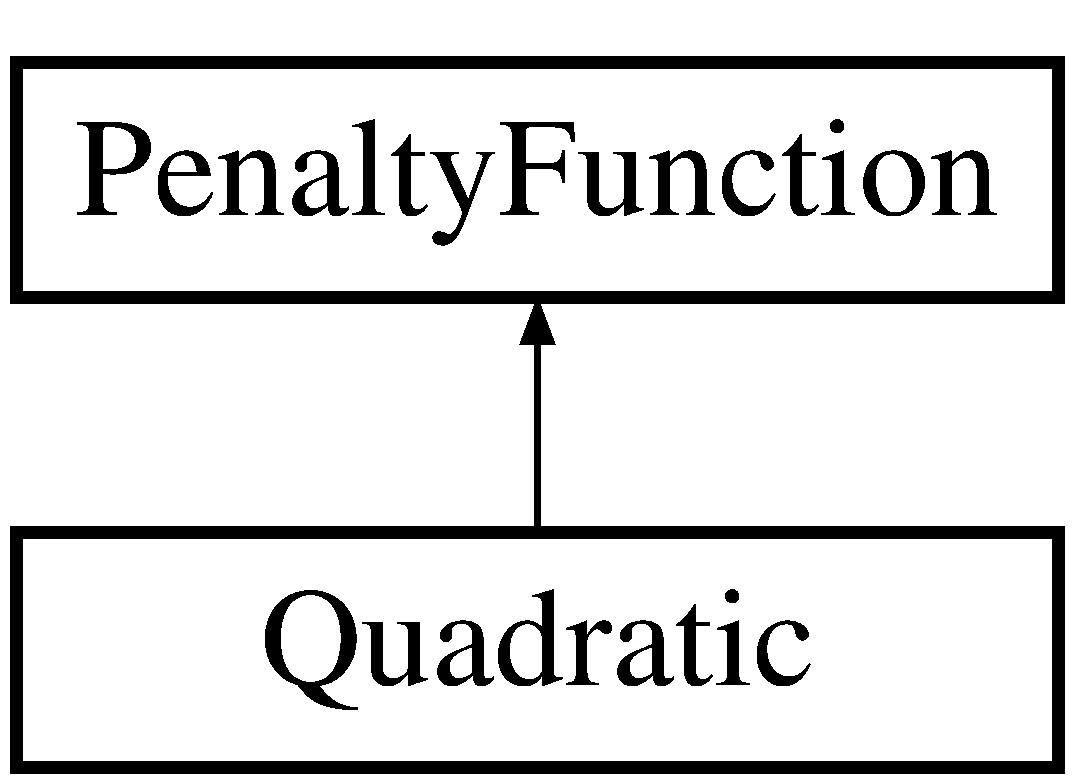
\includegraphics[height=2.000000cm]{class_penalty_function}
\end{center}
\end{figure}
\subsection*{Public Member Functions}
\begin{DoxyCompactItemize}
\item 
virtual double \hyperlink{class_penalty_function_a944230ce310515b1fe10972388c00042}{operator()} (const int x0, const int x1, const double y0, const double y1) const =0
\begin{DoxyCompactList}\small\item\em intersection operator \end{DoxyCompactList}\item 
virtual double \hyperlink{class_penalty_function_ad1f2cdbcfc85d0eaf3b734cafce60c48}{operator()} (const int x, const double y) const =0
\begin{DoxyCompactList}\small\item\em lower-\/envelope operator \end{DoxyCompactList}\item 
virtual \hyperlink{class_penalty_function_ac97741baf27aa9e506f430338f460498}{$\sim$\-Penalty\-Function} ()
\end{DoxyCompactItemize}


\subsection{Detailed Description}
an interface for penalty functions to be passed to \hyperlink{class_distance_transform}{Distance\-Transform} 

This penalty function interface defines the methods required by a function to be used in \hyperlink{class_distance_transform}{Distance\-Transform}. The function must be convex, so that the intersection between two such functions upholds a set of invariants. 

\subsection{Constructor \& Destructor Documentation}
\hypertarget{class_penalty_function_ac97741baf27aa9e506f430338f460498}{\index{Penalty\-Function@{Penalty\-Function}!$\sim$\-Penalty\-Function@{$\sim$\-Penalty\-Function}}
\index{$\sim$\-Penalty\-Function@{$\sim$\-Penalty\-Function}!PenaltyFunction@{Penalty\-Function}}
\subsubsection[{$\sim$\-Penalty\-Function}]{\setlength{\rightskip}{0pt plus 5cm}virtual Penalty\-Function\-::$\sim$\-Penalty\-Function (
\begin{DoxyParamCaption}
{}
\end{DoxyParamCaption}
)\hspace{0.3cm}{\ttfamily [inline]}, {\ttfamily [virtual]}}}\label{class_penalty_function_ac97741baf27aa9e506f430338f460498}


\subsection{Member Function Documentation}
\hypertarget{class_penalty_function_a944230ce310515b1fe10972388c00042}{\index{Penalty\-Function@{Penalty\-Function}!operator()@{operator()}}
\index{operator()@{operator()}!PenaltyFunction@{Penalty\-Function}}
\subsubsection[{operator()}]{\setlength{\rightskip}{0pt plus 5cm}virtual double Penalty\-Function\-::operator() (
\begin{DoxyParamCaption}
\item[{const int}]{x0, }
\item[{const int}]{x1, }
\item[{const double}]{y0, }
\item[{const double}]{y1}
\end{DoxyParamCaption}
) const\hspace{0.3cm}{\ttfamily [pure virtual]}}}\label{class_penalty_function_a944230ce310515b1fe10972388c00042}


intersection operator 

The intersection operator is used to find the height of intersection between two offset penalty functions.


\begin{DoxyParams}{Parameters}
{\em x0} & the location of the first function \\
\hline
{\em x1} & the location of the second function \\
\hline
{\em y0} & the height of the underlying sampled function at x0 \\
\hline
{\em y1} & the height of the underlying sampled function at x1 \\
\hline
\end{DoxyParams}
\begin{DoxyReturn}{Returns}
the height of the point of intersection 
\end{DoxyReturn}


Implemented in \hyperlink{class_quadratic_ad074fa92b51e0590f6621b60ac01219a}{Quadratic}.

\hypertarget{class_penalty_function_ad1f2cdbcfc85d0eaf3b734cafce60c48}{\index{Penalty\-Function@{Penalty\-Function}!operator()@{operator()}}
\index{operator()@{operator()}!PenaltyFunction@{Penalty\-Function}}
\subsubsection[{operator()}]{\setlength{\rightskip}{0pt plus 5cm}virtual double Penalty\-Function\-::operator() (
\begin{DoxyParamCaption}
\item[{const int}]{x, }
\item[{const double}]{y}
\end{DoxyParamCaption}
) const\hspace{0.3cm}{\ttfamily [pure virtual]}}}\label{class_penalty_function_ad1f2cdbcfc85d0eaf3b734cafce60c48}


lower-\/envelope operator 

given the pixel location of the lower envelope, calculate the true function height at that point 
\begin{DoxyParams}{Parameters}
{\em x} & the lower envelope's location on the function \\
\hline
{\em y} & the height of the underlying sampled point \\
\hline
\end{DoxyParams}
\begin{DoxyReturn}{Returns}

\end{DoxyReturn}


Implemented in \hyperlink{class_quadratic_ae1f3f6d71209aafe6bb1636a8c17489c}{Quadratic}.



The documentation for this class was generated from the following file\-:\begin{DoxyCompactItemize}
\item 
/\-Users/m29474/\-Desktop/code/openbr/3rdparty/\-Parts\-Based\-Detector/include/\hyperlink{_distance_transform_8hpp}{Distance\-Transform.\-hpp}\end{DoxyCompactItemize}

\hypertarget{class_point_cloud_clusterer}{\section{Point\-Cloud\-Clusterer$<$ Point\-Type $>$ Class Template Reference}
\label{class_point_cloud_clusterer}\index{Point\-Cloud\-Clusterer$<$ Point\-Type $>$@{Point\-Cloud\-Clusterer$<$ Point\-Type $>$}}
}


{\ttfamily \#include $<$Point\-Cloud\-Clusterer.\-h$>$}

\subsection*{Public Types}
\begin{DoxyCompactItemize}
\item 
typedef pcl\-::\-Point\-Cloud\\*
$<$ Point\-Type $>$ \hyperlink{class_point_cloud_clusterer_aeac82c7494ccf2580112ef55d7e30b39}{Point\-Cloud}
\item 
typedef Point\-Cloud\-::\-Const\-Ptr \hyperlink{class_point_cloud_clusterer_a042579611b15a7ae275603b624df3968}{Point\-Cloud\-Const\-Ptr}
\item 
typedef boost\-::function\\*
$<$ cv\-::\-Point3d(cv\-::\-Point)$>$ \hyperlink{class_point_cloud_clusterer_adc13c5f02a2a888f33eedbc33188f202}{Point\-Project\-Func}
\end{DoxyCompactItemize}
\subsection*{Static Public Member Functions}
\begin{DoxyCompactItemize}
\item 
static void \hyperlink{class_point_cloud_clusterer_add62f99dcb8932a59758ac974611fb3d}{compute\-Bounding\-Boxes} (const std\-::vector$<$ \hyperlink{class_candidate}{Candidate} $>$ \&candidates, const cv\-::\-Mat \&rgb, const cv\-::\-Mat \&depth, \hyperlink{class_point_cloud_clusterer_adc13c5f02a2a888f33eedbc33188f202}{Point\-Project\-Func} camera\-\_\-model\-\_\-projecter, const typename Point\-Cloud\-::\-Const\-Ptr cloud, std\-::vector$<$ \hyperlink{_rect3_8hpp_a05172c5a86161981edfe197f57415582}{Rect3d} $>$ \&bounding\-\_\-boxes, std\-::vector$<$ \hyperlink{class_point_cloud_clusterer_aeac82c7494ccf2580112ef55d7e30b39}{Point\-Cloud} $>$ \&parts\-\_\-centers)
\begin{DoxyCompactList}\small\item\em this function computes the 3\-D bounding boxes around the candidates \end{DoxyCompactList}\item 
static void \hyperlink{class_point_cloud_clusterer_a8c2ad76e5ddbea4277a03bd105f2ec9e}{cluster\-Objects} (const \hyperlink{class_point_cloud_clusterer_a042579611b15a7ae275603b624df3968}{Point\-Cloud\-Const\-Ptr} cloud, const std\-::vector$<$ \hyperlink{_rect3_8hpp_a05172c5a86161981edfe197f57415582}{Rect3d} $>$ \&bounding\-\_\-boxes, std\-::vector$<$ \hyperlink{class_point_cloud_clusterer_aeac82c7494ccf2580112ef55d7e30b39}{Point\-Cloud} $>$ \&object\-\_\-clusters, std\-::vector$<$ Point\-Type $>$ \&object\-\_\-centers)
\begin{DoxyCompactList}\small\item\em this function uses the 3\-D bounding boxes to segment and extract a point cluster for each detected object \end{DoxyCompactList}\item 
static void \hyperlink{class_point_cloud_clusterer_a262d27615d949a6923ca0b581dc59f1c}{organized\-Multiplane\-Segmentation} (const \hyperlink{class_point_cloud_clusterer_a042579611b15a7ae275603b624df3968}{Point\-Cloud\-Const\-Ptr} \&cloud, \hyperlink{class_point_cloud_clusterer_aeac82c7494ccf2580112ef55d7e30b39}{Point\-Cloud} \&cloud\-\_\-no\-\_\-plane)
\begin{DoxyCompactList}\small\item\em this function removes planes from the (organized) input cloud \end{DoxyCompactList}\end{DoxyCompactItemize}


\subsection{Member Typedef Documentation}
\hypertarget{class_point_cloud_clusterer_aeac82c7494ccf2580112ef55d7e30b39}{\index{Point\-Cloud\-Clusterer@{Point\-Cloud\-Clusterer}!Point\-Cloud@{Point\-Cloud}}
\index{Point\-Cloud@{Point\-Cloud}!PointCloudClusterer@{Point\-Cloud\-Clusterer}}
\subsubsection[{Point\-Cloud}]{\setlength{\rightskip}{0pt plus 5cm}template$<$typename Point\-Type $>$ typedef pcl\-::\-Point\-Cloud$<$Point\-Type$>$ {\bf Point\-Cloud\-Clusterer}$<$ Point\-Type $>$\-::{\bf Point\-Cloud}}}\label{class_point_cloud_clusterer_aeac82c7494ccf2580112ef55d7e30b39}
\hypertarget{class_point_cloud_clusterer_a042579611b15a7ae275603b624df3968}{\index{Point\-Cloud\-Clusterer@{Point\-Cloud\-Clusterer}!Point\-Cloud\-Const\-Ptr@{Point\-Cloud\-Const\-Ptr}}
\index{Point\-Cloud\-Const\-Ptr@{Point\-Cloud\-Const\-Ptr}!PointCloudClusterer@{Point\-Cloud\-Clusterer}}
\subsubsection[{Point\-Cloud\-Const\-Ptr}]{\setlength{\rightskip}{0pt plus 5cm}template$<$typename Point\-Type $>$ typedef Point\-Cloud\-::\-Const\-Ptr {\bf Point\-Cloud\-Clusterer}$<$ Point\-Type $>$\-::{\bf Point\-Cloud\-Const\-Ptr}}}\label{class_point_cloud_clusterer_a042579611b15a7ae275603b624df3968}
\hypertarget{class_point_cloud_clusterer_adc13c5f02a2a888f33eedbc33188f202}{\index{Point\-Cloud\-Clusterer@{Point\-Cloud\-Clusterer}!Point\-Project\-Func@{Point\-Project\-Func}}
\index{Point\-Project\-Func@{Point\-Project\-Func}!PointCloudClusterer@{Point\-Cloud\-Clusterer}}
\subsubsection[{Point\-Project\-Func}]{\setlength{\rightskip}{0pt plus 5cm}template$<$typename Point\-Type $>$ typedef boost\-::function$<$cv\-::\-Point3d(cv\-::\-Point)$>$ {\bf Point\-Cloud\-Clusterer}$<$ Point\-Type $>$\-::{\bf Point\-Project\-Func}}}\label{class_point_cloud_clusterer_adc13c5f02a2a888f33eedbc33188f202}


\subsection{Member Function Documentation}
\hypertarget{class_point_cloud_clusterer_a8c2ad76e5ddbea4277a03bd105f2ec9e}{\index{Point\-Cloud\-Clusterer@{Point\-Cloud\-Clusterer}!cluster\-Objects@{cluster\-Objects}}
\index{cluster\-Objects@{cluster\-Objects}!PointCloudClusterer@{Point\-Cloud\-Clusterer}}
\subsubsection[{cluster\-Objects}]{\setlength{\rightskip}{0pt plus 5cm}template$<$typename Point\-Type $>$ void {\bf Point\-Cloud\-Clusterer}$<$ Point\-Type $>$\-::cluster\-Objects (
\begin{DoxyParamCaption}
\item[{const {\bf Point\-Cloud\-Const\-Ptr}}]{cloud, }
\item[{const std\-::vector$<$ {\bf Rect3d} $>$ \&}]{bounding\-\_\-boxes, }
\item[{std\-::vector$<$ {\bf Point\-Cloud} $>$ \&}]{object\-\_\-clusters, }
\item[{std\-::vector$<$ Point\-Type $>$ \&}]{object\-\_\-centers}
\end{DoxyParamCaption}
)\hspace{0.3cm}{\ttfamily [static]}}}\label{class_point_cloud_clusterer_a8c2ad76e5ddbea4277a03bd105f2ec9e}


this function uses the 3\-D bounding boxes to segment and extract a point cluster for each detected object 


\begin{DoxyParams}{Parameters}
{\em cloud} & the input point cloud \\
\hline
{\em bounding\-\_\-boxes} & the 3\-D bunding boxes \\
\hline
{\em object\-\_\-clusters} & a vector of Point\-Clouds is returned, a cluster for each bounding box \\
\hline
{\em object\-\_\-centers} & the centroid of each cluster \\
\hline
\end{DoxyParams}
\hypertarget{class_point_cloud_clusterer_add62f99dcb8932a59758ac974611fb3d}{\index{Point\-Cloud\-Clusterer@{Point\-Cloud\-Clusterer}!compute\-Bounding\-Boxes@{compute\-Bounding\-Boxes}}
\index{compute\-Bounding\-Boxes@{compute\-Bounding\-Boxes}!PointCloudClusterer@{Point\-Cloud\-Clusterer}}
\subsubsection[{compute\-Bounding\-Boxes}]{\setlength{\rightskip}{0pt plus 5cm}template$<$typename Point\-Type $>$ void {\bf Point\-Cloud\-Clusterer}$<$ Point\-Type $>$\-::compute\-Bounding\-Boxes (
\begin{DoxyParamCaption}
\item[{const std\-::vector$<$ {\bf Candidate} $>$ \&}]{candidates, }
\item[{const cv\-::\-Mat \&}]{rgb, }
\item[{const cv\-::\-Mat \&}]{depth, }
\item[{{\bf Point\-Project\-Func}}]{camera\-\_\-model\-\_\-projecter, }
\item[{const typename Point\-Cloud\-::\-Const\-Ptr}]{cloud, }
\item[{std\-::vector$<$ {\bf Rect3d} $>$ \&}]{bounding\-\_\-boxes, }
\item[{std\-::vector$<$ {\bf Point\-Cloud} $>$ \&}]{parts\-\_\-centers}
\end{DoxyParamCaption}
)\hspace{0.3cm}{\ttfamily [static]}}}\label{class_point_cloud_clusterer_add62f99dcb8932a59758ac974611fb3d}


this function computes the 3\-D bounding boxes around the candidates 


\begin{DoxyParams}{Parameters}
{\em candidates} & the candidates returned by the parts based detector \\
\hline
{\em rgb} & the rgb image \\
\hline
{\em depth} & the depth image \\
\hline
{\em camera\-\_\-model\-\_\-projecter} & the function that projects the 2d pixel into a 3d ray \\
\hline
{\em cloud} & the pointcloud \\
\hline
{\em bounding\-\_\-boxes} & the 3\-D bounding boxes for each candidate \\
\hline
{\em parts\-\_\-centers} & a point cloud for each candidate, each point represents the center for a part \\
\hline
\end{DoxyParams}
\hypertarget{class_point_cloud_clusterer_a262d27615d949a6923ca0b581dc59f1c}{\index{Point\-Cloud\-Clusterer@{Point\-Cloud\-Clusterer}!organized\-Multiplane\-Segmentation@{organized\-Multiplane\-Segmentation}}
\index{organized\-Multiplane\-Segmentation@{organized\-Multiplane\-Segmentation}!PointCloudClusterer@{Point\-Cloud\-Clusterer}}
\subsubsection[{organized\-Multiplane\-Segmentation}]{\setlength{\rightskip}{0pt plus 5cm}template$<$typename Point\-Type $>$ void {\bf Point\-Cloud\-Clusterer}$<$ Point\-Type $>$\-::organized\-Multiplane\-Segmentation (
\begin{DoxyParamCaption}
\item[{const {\bf Point\-Cloud\-Const\-Ptr} \&}]{cloud, }
\item[{{\bf Point\-Cloud} \&}]{cloud\-\_\-no\-\_\-plane}
\end{DoxyParamCaption}
)\hspace{0.3cm}{\ttfamily [static]}}}\label{class_point_cloud_clusterer_a262d27615d949a6923ca0b581dc59f1c}


this function removes planes from the (organized) input cloud 


\begin{DoxyParams}{Parameters}
{\em cloud} & the input point cloud \\
\hline
{\em cloud\-\_\-no\-\_\-plane} & the filtered input cloud (planes removed) \\
\hline
\end{DoxyParams}


The documentation for this class was generated from the following files\-:\begin{DoxyCompactItemize}
\item 
/\-Users/m29474/\-Desktop/code/openbr/3rdparty/\-Parts\-Based\-Detector/include/\hyperlink{_point_cloud_clusterer_8h}{Point\-Cloud\-Clusterer.\-h}\item 
/\-Users/m29474/\-Desktop/code/openbr/3rdparty/\-Parts\-Based\-Detector/include/\hyperlink{_point_cloud_clusterer_8hpp}{Point\-Cloud\-Clusterer.\-hpp}\end{DoxyCompactItemize}

\hypertarget{class_quadratic}{\section{Quadratic Class Reference}
\label{class_quadratic}\index{Quadratic@{Quadratic}}
}


quadratic penalty function  




{\ttfamily \#include $<$Distance\-Transform.\-hpp$>$}

Inheritance diagram for Quadratic\-:\begin{figure}[H]
\begin{center}
\leavevmode
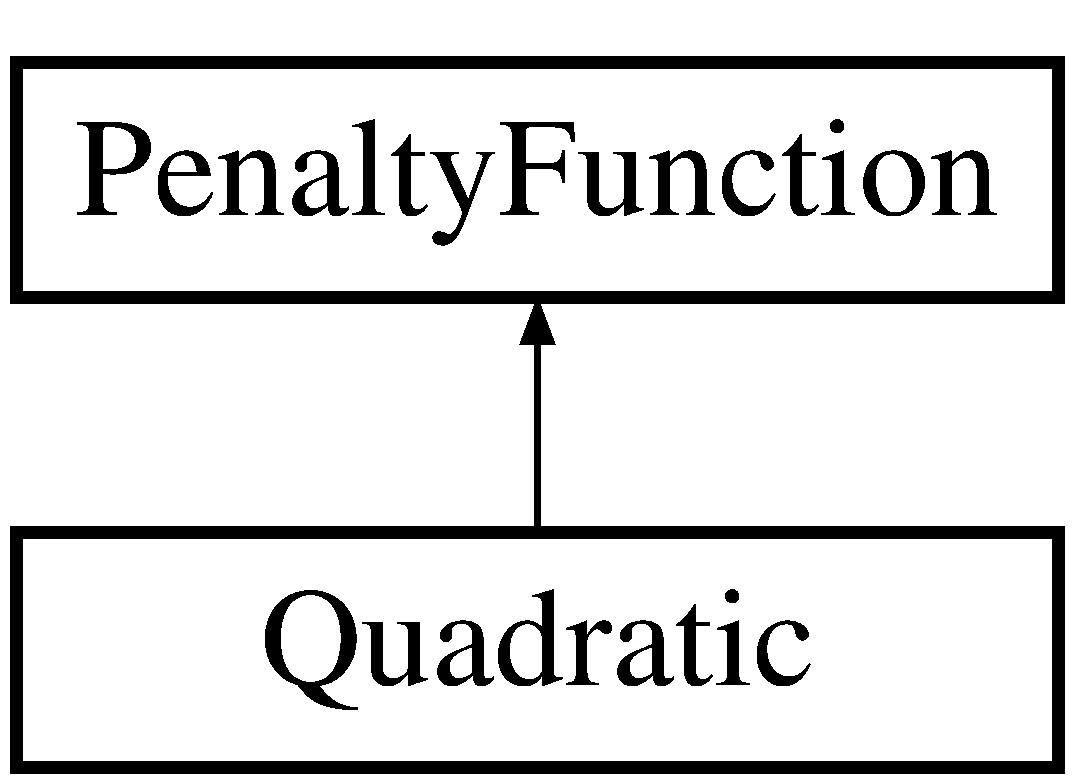
\includegraphics[height=2.000000cm]{class_quadratic}
\end{center}
\end{figure}
\subsection*{Public Member Functions}
\begin{DoxyCompactItemize}
\item 
\hyperlink{class_quadratic_aa5d5e8e58a9d0aaf332e6b8b879430b8}{Quadratic} (double \-\_\-a, double \-\_\-b)
\item 
double \hyperlink{class_quadratic_ad074fa92b51e0590f6621b60ac01219a}{operator()} (const int x0, const int x1, const double y0, const double y1) const 
\begin{DoxyCompactList}\small\item\em intersection operator \end{DoxyCompactList}\item 
double \hyperlink{class_quadratic_ae1f3f6d71209aafe6bb1636a8c17489c}{operator()} (const int x, const double y) const 
\begin{DoxyCompactList}\small\item\em lower-\/envelope operator \end{DoxyCompactList}\end{DoxyCompactItemize}
\subsection*{Data Fields}
\begin{DoxyCompactItemize}
\item 
double const \hyperlink{class_quadratic_a3784ebac36b04b9195d44d6d5bc8933a}{a}
\item 
double const \hyperlink{class_quadratic_a1df1154ac27afe4533b5b695831ed23a}{b}
\end{DoxyCompactItemize}
\subsection*{Private Member Functions}
\begin{DoxyCompactItemize}
\item 
int \hyperlink{class_quadratic_a0fd7e9cc0ce3028a7db656ec0cb8f84f}{square} (int x) const 
\end{DoxyCompactItemize}


\subsection{Detailed Description}
quadratic penalty function 

This class implements a Euclidean distance penalty function which manifests as a quadratic function 

\subsection{Constructor \& Destructor Documentation}
\hypertarget{class_quadratic_aa5d5e8e58a9d0aaf332e6b8b879430b8}{\index{Quadratic@{Quadratic}!Quadratic@{Quadratic}}
\index{Quadratic@{Quadratic}!Quadratic@{Quadratic}}
\subsubsection[{Quadratic}]{\setlength{\rightskip}{0pt plus 5cm}Quadratic\-::\-Quadratic (
\begin{DoxyParamCaption}
\item[{double}]{\-\_\-a, }
\item[{double}]{\-\_\-b}
\end{DoxyParamCaption}
)\hspace{0.3cm}{\ttfamily [inline]}}}\label{class_quadratic_aa5d5e8e58a9d0aaf332e6b8b879430b8}


\subsection{Member Function Documentation}
\hypertarget{class_quadratic_ad074fa92b51e0590f6621b60ac01219a}{\index{Quadratic@{Quadratic}!operator()@{operator()}}
\index{operator()@{operator()}!Quadratic@{Quadratic}}
\subsubsection[{operator()}]{\setlength{\rightskip}{0pt plus 5cm}double Quadratic\-::operator() (
\begin{DoxyParamCaption}
\item[{const int}]{x0, }
\item[{const int}]{x1, }
\item[{const double}]{y0, }
\item[{const double}]{y1}
\end{DoxyParamCaption}
) const\hspace{0.3cm}{\ttfamily [inline]}, {\ttfamily [virtual]}}}\label{class_quadratic_ad074fa92b51e0590f6621b60ac01219a}


intersection operator 

The intersection operator is used to find the height of intersection between two offset penalty functions.


\begin{DoxyParams}{Parameters}
{\em x0} & the location of the first function \\
\hline
{\em x1} & the location of the second function \\
\hline
{\em y0} & the height of the underlying sampled function at x0 \\
\hline
{\em y1} & the height of the underlying sampled function at x1 \\
\hline
\end{DoxyParams}
\begin{DoxyReturn}{Returns}
the height of the point of intersection 
\end{DoxyReturn}


Implements \hyperlink{class_penalty_function_a944230ce310515b1fe10972388c00042}{Penalty\-Function}.

\hypertarget{class_quadratic_ae1f3f6d71209aafe6bb1636a8c17489c}{\index{Quadratic@{Quadratic}!operator()@{operator()}}
\index{operator()@{operator()}!Quadratic@{Quadratic}}
\subsubsection[{operator()}]{\setlength{\rightskip}{0pt plus 5cm}double Quadratic\-::operator() (
\begin{DoxyParamCaption}
\item[{const int}]{x, }
\item[{const double}]{y}
\end{DoxyParamCaption}
) const\hspace{0.3cm}{\ttfamily [inline]}, {\ttfamily [virtual]}}}\label{class_quadratic_ae1f3f6d71209aafe6bb1636a8c17489c}


lower-\/envelope operator 

given the pixel location of the lower envelope, calculate the true function height at that point 
\begin{DoxyParams}{Parameters}
{\em x} & the lower envelope's location on the function \\
\hline
{\em y} & the height of the underlying sampled point \\
\hline
\end{DoxyParams}
\begin{DoxyReturn}{Returns}

\end{DoxyReturn}


Implements \hyperlink{class_penalty_function_ad1f2cdbcfc85d0eaf3b734cafce60c48}{Penalty\-Function}.

\hypertarget{class_quadratic_a0fd7e9cc0ce3028a7db656ec0cb8f84f}{\index{Quadratic@{Quadratic}!square@{square}}
\index{square@{square}!Quadratic@{Quadratic}}
\subsubsection[{square}]{\setlength{\rightskip}{0pt plus 5cm}int Quadratic\-::square (
\begin{DoxyParamCaption}
\item[{int}]{x}
\end{DoxyParamCaption}
) const\hspace{0.3cm}{\ttfamily [inline]}, {\ttfamily [private]}}}\label{class_quadratic_a0fd7e9cc0ce3028a7db656ec0cb8f84f}


\subsection{Field Documentation}
\hypertarget{class_quadratic_a3784ebac36b04b9195d44d6d5bc8933a}{\index{Quadratic@{Quadratic}!a@{a}}
\index{a@{a}!Quadratic@{Quadratic}}
\subsubsection[{a}]{\setlength{\rightskip}{0pt plus 5cm}double const Quadratic\-::a}}\label{class_quadratic_a3784ebac36b04b9195d44d6d5bc8933a}
\hypertarget{class_quadratic_a1df1154ac27afe4533b5b695831ed23a}{\index{Quadratic@{Quadratic}!b@{b}}
\index{b@{b}!Quadratic@{Quadratic}}
\subsubsection[{b}]{\setlength{\rightskip}{0pt plus 5cm}double const Quadratic\-::b}}\label{class_quadratic_a1df1154ac27afe4533b5b695831ed23a}


The documentation for this class was generated from the following file\-:\begin{DoxyCompactItemize}
\item 
/\-Users/m29474/\-Desktop/code/openbr/3rdparty/\-Parts\-Based\-Detector/include/\hyperlink{_distance_transform_8hpp}{Distance\-Transform.\-hpp}\end{DoxyCompactItemize}

\hypertarget{class_rect3__}{\section{Rect3\-\_\-$<$ T $>$ Class Template Reference}
\label{class_rect3__}\index{Rect3\-\_\-$<$ T $>$@{Rect3\-\_\-$<$ T $>$}}
}


3\-D rectangle class This class implements a 3\-D rectangle which provides similar functionality to the Open\-C\-V Rect\-\_\- class, but in 3-\/space  




{\ttfamily \#include $<$Rect3.\-hpp$>$}

\subsection*{Public Member Functions}
\begin{DoxyCompactItemize}
\item 
\hyperlink{class_rect3___a5c3ceb93ece38ee7145436652670cef8}{Rect3\-\_\-} ()
\begin{DoxyCompactList}\small\item\em default constructor \end{DoxyCompactList}\item 
\hyperlink{class_rect3___a5f055c2312c2426746e8c7421c11535f}{Rect3\-\_\-} (T \-\_\-x, T \-\_\-y, T \-\_\-z, T \-\_\-height, T \-\_\-width, T \-\_\-depth)
\begin{DoxyCompactList}\small\item\em constructor with primitive arguments \end{DoxyCompactList}\item 
\hyperlink{class_rect3___addad14c64f04aae61ab4ef7be23e72c4}{Rect3\-\_\-} (const \hyperlink{class_rect3__}{Rect3\-\_\-}$<$ T $>$ \&r)
\begin{DoxyCompactList}\small\item\em copy constructor \end{DoxyCompactList}\item 
\hyperlink{class_rect3___a8ceab5818fcd871fc373437084a84157}{Rect3\-\_\-} (const cv\-::\-Point3\-\_\-$<$ T $>$ pt1, const cv\-::\-Point3\-\_\-$<$ T $>$ pt2)
\begin{DoxyCompactList}\small\item\em constructor using points \end{DoxyCompactList}\item 
\hyperlink{class_rect3__}{Rect3\-\_\-}$<$ T $>$ \& \hyperlink{class_rect3___a5f5849c81f0561292c78d7df6e68f569}{operator+} (const cv\-::\-Point3\-\_\-$<$ T $>$ \&r)
\begin{DoxyCompactList}\small\item\em equals operator \end{DoxyCompactList}\item 
\hyperlink{class_rect3__}{Rect3\-\_\-}$<$ T $>$ \& \hyperlink{class_rect3___accafb3f3d3ddea87cab8ed9a274480dd}{operator-\/} (const cv\-::\-Point3\-\_\-$<$ T $>$ \&r)
\begin{DoxyCompactList}\small\item\em subtraction operator \end{DoxyCompactList}\item 
\hyperlink{class_rect3__}{Rect3\-\_\-}$<$ T $>$ \& \hyperlink{class_rect3___a7b3e73a2456c26db0ba85efbf1eac087}{operator+=} (const cv\-::\-Point3\-\_\-$<$ T $>$ \&r)
\begin{DoxyCompactList}\small\item\em addition in-\/place \end{DoxyCompactList}\item 
\hyperlink{class_rect3__}{Rect3\-\_\-}$<$ T $>$ \& \hyperlink{class_rect3___a3a626255017a7cef76e065c51ef1504f}{operator-\/=} (const cv\-::\-Point3\-\_\-$<$ T $>$ \&r)
\begin{DoxyCompactList}\small\item\em subtraction in-\/place \end{DoxyCompactList}\item 
\hyperlink{class_rect3__}{Rect3\-\_\-}$<$ T $>$ \& \hyperlink{class_rect3___a24609371fde6d5c8383dbb210bb75b5e}{operator\&} (const \hyperlink{class_rect3__}{Rect3\-\_\-}$<$ T $>$ r)
\begin{DoxyCompactList}\small\item\em intersection operator \end{DoxyCompactList}\item 
\hyperlink{class_rect3__}{Rect3\-\_\-}$<$ T $>$ \& \hyperlink{class_rect3___a0f988dcf6a9ad19243844abf4acba653}{operator$|$} (const \hyperlink{class_rect3__}{Rect3\-\_\-}$<$ T $>$ r)
\begin{DoxyCompactList}\small\item\em convex hull operator \end{DoxyCompactList}\item 
\hyperlink{class_rect3___a4f49b82908b88ed545690bfff932ea30}{operator cv\-::\-Rect\-\_\-$<$ T $>$} ()
\begin{DoxyCompactList}\small\item\em down-\/conversion to a Rect \end{DoxyCompactList}\item 
cv\-::\-Point3\-\_\-$<$ T $>$ \hyperlink{class_rect3___a8df208aa3d316ea706a529db292d1a0f}{tl} () const 
\begin{DoxyCompactList}\small\item\em the top left corner in 3-\/space \end{DoxyCompactList}\item 
cv\-::\-Point3\-\_\-$<$ T $>$ \hyperlink{class_rect3___a253d895d86ec7718351f29ff3cd0cd27}{br} () const 
\begin{DoxyCompactList}\small\item\em the bottom right corner in 3-\/space \end{DoxyCompactList}\item 
T \hyperlink{class_rect3___a766842fae2533d47ccf9b7fb428670c8}{volume} () const 
\begin{DoxyCompactList}\small\item\em the volume of the encapsulated area \end{DoxyCompactList}\item 
bool \hyperlink{class_rect3___ad9928349a9a8bca8f98a1bf1cab676e9}{contains} (const cv\-::\-Point3\-\_\-$<$ T $>$ \&pt) const 
\begin{DoxyCompactList}\small\item\em check whether the prism contains the 3\-D-\/point \end{DoxyCompactList}\item 
cv\-::\-Point3\-\_\-$<$ T $>$ \hyperlink{class_rect3___addafb9e6380c9a3ffd4f394d311c59b6}{centroid} () const 
\begin{DoxyCompactList}\small\item\em get the centroid of the prism \end{DoxyCompactList}\item 
virtual \hyperlink{class_rect3___a297683142c5197991bfaabdb2305a37c}{$\sim$\-Rect3\-\_\-} ()
\begin{DoxyCompactList}\small\item\em destructor \end{DoxyCompactList}\end{DoxyCompactItemize}
\subsection*{Static Public Member Functions}
\begin{DoxyCompactItemize}
\item 
static \hyperlink{class_rect3__}{Rect3\-\_\-}$<$ T $>$ \hyperlink{class_rect3___a65f8ac50cb83bd238d0a20fe7f63fc31}{convex\-Hull} (const \hyperlink{class_rect3__}{Rect3\-\_\-}$<$ T $>$ \&r1, const \hyperlink{class_rect3__}{Rect3\-\_\-}$<$ T $>$ \&r2)
\begin{DoxyCompactList}\small\item\em convex hull of two rectangles The rectangular convex hull is defined as the minimum bounding rectangle that completely encapsulates both rectangles (in 3-\/space) \end{DoxyCompactList}\item 
static \hyperlink{class_rect3__}{Rect3\-\_\-}$<$ T $>$ \hyperlink{class_rect3___af928b65e6d154f1d196725c18820ab2c}{convex\-Hull} (const std\-::vector$<$ \hyperlink{class_rect3__}{Rect3\-\_\-}$<$ T $>$ $>$ \&r)
\begin{DoxyCompactList}\small\item\em convex hull of two rectangles The rectangular convex hull is defined as the minimum bounding rectangle that completely encapsulates both rectangles (in 3-\/space) \end{DoxyCompactList}\item 
static \hyperlink{class_rect3__}{Rect3\-\_\-}$<$ T $>$ \hyperlink{class_rect3___ade590c7c83be16b840539a2dede75f08}{intersection} (const \hyperlink{class_rect3__}{Rect3\-\_\-}$<$ T $>$ \&r1, const \hyperlink{class_rect3__}{Rect3\-\_\-}$<$ T $>$ \&r2)
\begin{DoxyCompactList}\small\item\em find the intersection of two rectangular prisms in 3-\/space \end{DoxyCompactList}\end{DoxyCompactItemize}
\subsection*{Data Fields}
\begin{DoxyCompactItemize}
\item 
T \hyperlink{class_rect3___a035f211c0c365a9dbd15436cb5448e31}{x}
\item 
T \hyperlink{class_rect3___ab2c61e4e318bc064eb8bb707b699cbb6}{y}
\item 
T \hyperlink{class_rect3___a99bae7d4f2bf0af6a3ffbfb0fa752b9e}{z}
\item 
T \hyperlink{class_rect3___a4f10fdcf15fe8cdb6b01a9b90d56ebe5}{height}
\item 
T \hyperlink{class_rect3___a780cbb24a81d6bbfff26c2ac6660beb8}{width}
\item 
T \hyperlink{class_rect3___a73850e016f7e8152e47d430239c47cc2}{depth}
\end{DoxyCompactItemize}
\subsection*{Friends}
\begin{DoxyCompactItemize}
\item 
std\-::ostream \& \hyperlink{class_rect3___af7a3194527b2890e66a2677897434cd9}{operator$<$$<$} (std\-::ostream \&stream, const \hyperlink{class_rect3__}{Rect3\-\_\-}$<$ T $>$ \&r)
\begin{DoxyCompactList}\small\item\em stream insertion operator \end{DoxyCompactList}\end{DoxyCompactItemize}


\subsection{Detailed Description}
\subsubsection*{template$<$typename T$>$class Rect3\-\_\-$<$ T $>$}

3\-D rectangle class This class implements a 3\-D rectangle which provides similar functionality to the Open\-C\-V Rect\-\_\- class, but in 3-\/space 

\subsection{Constructor \& Destructor Documentation}
\hypertarget{class_rect3___a5c3ceb93ece38ee7145436652670cef8}{\index{Rect3\-\_\-@{Rect3\-\_\-}!Rect3\-\_\-@{Rect3\-\_\-}}
\index{Rect3\-\_\-@{Rect3\-\_\-}!Rect3_@{Rect3\-\_\-}}
\subsubsection[{Rect3\-\_\-}]{\setlength{\rightskip}{0pt plus 5cm}template$<$typename T$>$ {\bf Rect3\-\_\-}$<$ T $>$\-::{\bf Rect3\-\_\-} (
\begin{DoxyParamCaption}
{}
\end{DoxyParamCaption}
)\hspace{0.3cm}{\ttfamily [inline]}}}\label{class_rect3___a5c3ceb93ece38ee7145436652670cef8}


default constructor 

\hypertarget{class_rect3___a5f055c2312c2426746e8c7421c11535f}{\index{Rect3\-\_\-@{Rect3\-\_\-}!Rect3\-\_\-@{Rect3\-\_\-}}
\index{Rect3\-\_\-@{Rect3\-\_\-}!Rect3_@{Rect3\-\_\-}}
\subsubsection[{Rect3\-\_\-}]{\setlength{\rightskip}{0pt plus 5cm}template$<$typename T$>$ {\bf Rect3\-\_\-}$<$ T $>$\-::{\bf Rect3\-\_\-} (
\begin{DoxyParamCaption}
\item[{T}]{\-\_\-x, }
\item[{T}]{\-\_\-y, }
\item[{T}]{\-\_\-z, }
\item[{T}]{\-\_\-height, }
\item[{T}]{\-\_\-width, }
\item[{T}]{\-\_\-depth}
\end{DoxyParamCaption}
)\hspace{0.3cm}{\ttfamily [inline]}}}\label{class_rect3___a5f055c2312c2426746e8c7421c11535f}


constructor with primitive arguments 

\hypertarget{class_rect3___addad14c64f04aae61ab4ef7be23e72c4}{\index{Rect3\-\_\-@{Rect3\-\_\-}!Rect3\-\_\-@{Rect3\-\_\-}}
\index{Rect3\-\_\-@{Rect3\-\_\-}!Rect3_@{Rect3\-\_\-}}
\subsubsection[{Rect3\-\_\-}]{\setlength{\rightskip}{0pt plus 5cm}template$<$typename T$>$ {\bf Rect3\-\_\-}$<$ T $>$\-::{\bf Rect3\-\_\-} (
\begin{DoxyParamCaption}
\item[{const {\bf Rect3\-\_\-}$<$ T $>$ \&}]{r}
\end{DoxyParamCaption}
)\hspace{0.3cm}{\ttfamily [inline]}}}\label{class_rect3___addad14c64f04aae61ab4ef7be23e72c4}


copy constructor 

\hypertarget{class_rect3___a8ceab5818fcd871fc373437084a84157}{\index{Rect3\-\_\-@{Rect3\-\_\-}!Rect3\-\_\-@{Rect3\-\_\-}}
\index{Rect3\-\_\-@{Rect3\-\_\-}!Rect3_@{Rect3\-\_\-}}
\subsubsection[{Rect3\-\_\-}]{\setlength{\rightskip}{0pt plus 5cm}template$<$typename T$>$ {\bf Rect3\-\_\-}$<$ T $>$\-::{\bf Rect3\-\_\-} (
\begin{DoxyParamCaption}
\item[{const cv\-::\-Point3\-\_\-$<$ T $>$}]{pt1, }
\item[{const cv\-::\-Point3\-\_\-$<$ T $>$}]{pt2}
\end{DoxyParamCaption}
)\hspace{0.3cm}{\ttfamily [inline]}}}\label{class_rect3___a8ceab5818fcd871fc373437084a84157}


constructor using points 

\hypertarget{class_rect3___a297683142c5197991bfaabdb2305a37c}{\index{Rect3\-\_\-@{Rect3\-\_\-}!$\sim$\-Rect3\-\_\-@{$\sim$\-Rect3\-\_\-}}
\index{$\sim$\-Rect3\-\_\-@{$\sim$\-Rect3\-\_\-}!Rect3_@{Rect3\-\_\-}}
\subsubsection[{$\sim$\-Rect3\-\_\-}]{\setlength{\rightskip}{0pt plus 5cm}template$<$typename T$>$ virtual {\bf Rect3\-\_\-}$<$ T $>$\-::$\sim${\bf Rect3\-\_\-} (
\begin{DoxyParamCaption}
{}
\end{DoxyParamCaption}
)\hspace{0.3cm}{\ttfamily [inline]}, {\ttfamily [virtual]}}}\label{class_rect3___a297683142c5197991bfaabdb2305a37c}


destructor 



\subsection{Member Function Documentation}
\hypertarget{class_rect3___a253d895d86ec7718351f29ff3cd0cd27}{\index{Rect3\-\_\-@{Rect3\-\_\-}!br@{br}}
\index{br@{br}!Rect3_@{Rect3\-\_\-}}
\subsubsection[{br}]{\setlength{\rightskip}{0pt plus 5cm}template$<$typename T$>$ cv\-::\-Point3\-\_\-$<$T$>$ {\bf Rect3\-\_\-}$<$ T $>$\-::br (
\begin{DoxyParamCaption}
{}
\end{DoxyParamCaption}
) const\hspace{0.3cm}{\ttfamily [inline]}}}\label{class_rect3___a253d895d86ec7718351f29ff3cd0cd27}


the bottom right corner in 3-\/space 

\hypertarget{class_rect3___addafb9e6380c9a3ffd4f394d311c59b6}{\index{Rect3\-\_\-@{Rect3\-\_\-}!centroid@{centroid}}
\index{centroid@{centroid}!Rect3_@{Rect3\-\_\-}}
\subsubsection[{centroid}]{\setlength{\rightskip}{0pt plus 5cm}template$<$typename T$>$ cv\-::\-Point3\-\_\-$<$T$>$ {\bf Rect3\-\_\-}$<$ T $>$\-::centroid (
\begin{DoxyParamCaption}
{}
\end{DoxyParamCaption}
) const\hspace{0.3cm}{\ttfamily [inline]}}}\label{class_rect3___addafb9e6380c9a3ffd4f394d311c59b6}


get the centroid of the prism 

\hypertarget{class_rect3___ad9928349a9a8bca8f98a1bf1cab676e9}{\index{Rect3\-\_\-@{Rect3\-\_\-}!contains@{contains}}
\index{contains@{contains}!Rect3_@{Rect3\-\_\-}}
\subsubsection[{contains}]{\setlength{\rightskip}{0pt plus 5cm}template$<$typename T$>$ bool {\bf Rect3\-\_\-}$<$ T $>$\-::contains (
\begin{DoxyParamCaption}
\item[{const cv\-::\-Point3\-\_\-$<$ T $>$ \&}]{pt}
\end{DoxyParamCaption}
) const\hspace{0.3cm}{\ttfamily [inline]}}}\label{class_rect3___ad9928349a9a8bca8f98a1bf1cab676e9}


check whether the prism contains the 3\-D-\/point 

\hypertarget{class_rect3___a65f8ac50cb83bd238d0a20fe7f63fc31}{\index{Rect3\-\_\-@{Rect3\-\_\-}!convex\-Hull@{convex\-Hull}}
\index{convex\-Hull@{convex\-Hull}!Rect3_@{Rect3\-\_\-}}
\subsubsection[{convex\-Hull}]{\setlength{\rightskip}{0pt plus 5cm}template$<$typename T$>$ static {\bf Rect3\-\_\-}$<$T$>$ {\bf Rect3\-\_\-}$<$ T $>$\-::convex\-Hull (
\begin{DoxyParamCaption}
\item[{const {\bf Rect3\-\_\-}$<$ T $>$ \&}]{r1, }
\item[{const {\bf Rect3\-\_\-}$<$ T $>$ \&}]{r2}
\end{DoxyParamCaption}
)\hspace{0.3cm}{\ttfamily [inline]}, {\ttfamily [static]}}}\label{class_rect3___a65f8ac50cb83bd238d0a20fe7f63fc31}


convex hull of two rectangles The rectangular convex hull is defined as the minimum bounding rectangle that completely encapsulates both rectangles (in 3-\/space) 


\begin{DoxyParams}{Parameters}
{\em r1} & the first rectangular prism \\
\hline
{\em r2} & the second rectangular prism \\
\hline
\end{DoxyParams}
\begin{DoxyReturn}{Returns}
the rectangular prism convex hull 
\end{DoxyReturn}
\hypertarget{class_rect3___af928b65e6d154f1d196725c18820ab2c}{\index{Rect3\-\_\-@{Rect3\-\_\-}!convex\-Hull@{convex\-Hull}}
\index{convex\-Hull@{convex\-Hull}!Rect3_@{Rect3\-\_\-}}
\subsubsection[{convex\-Hull}]{\setlength{\rightskip}{0pt plus 5cm}template$<$typename T$>$ static {\bf Rect3\-\_\-}$<$T$>$ {\bf Rect3\-\_\-}$<$ T $>$\-::convex\-Hull (
\begin{DoxyParamCaption}
\item[{const std\-::vector$<$ {\bf Rect3\-\_\-}$<$ T $>$ $>$ \&}]{r}
\end{DoxyParamCaption}
)\hspace{0.3cm}{\ttfamily [inline]}, {\ttfamily [static]}}}\label{class_rect3___af928b65e6d154f1d196725c18820ab2c}


convex hull of two rectangles The rectangular convex hull is defined as the minimum bounding rectangle that completely encapsulates both rectangles (in 3-\/space) 


\begin{DoxyParams}{Parameters}
{\em r} & a std\-::vector of rectangular prisms \\
\hline
\end{DoxyParams}
\begin{DoxyReturn}{Returns}
the rectangular prism convex hull 
\end{DoxyReturn}
\hypertarget{class_rect3___ade590c7c83be16b840539a2dede75f08}{\index{Rect3\-\_\-@{Rect3\-\_\-}!intersection@{intersection}}
\index{intersection@{intersection}!Rect3_@{Rect3\-\_\-}}
\subsubsection[{intersection}]{\setlength{\rightskip}{0pt plus 5cm}template$<$typename T$>$ static {\bf Rect3\-\_\-}$<$T$>$ {\bf Rect3\-\_\-}$<$ T $>$\-::intersection (
\begin{DoxyParamCaption}
\item[{const {\bf Rect3\-\_\-}$<$ T $>$ \&}]{r1, }
\item[{const {\bf Rect3\-\_\-}$<$ T $>$ \&}]{r2}
\end{DoxyParamCaption}
)\hspace{0.3cm}{\ttfamily [inline]}, {\ttfamily [static]}}}\label{class_rect3___ade590c7c83be16b840539a2dede75f08}


find the intersection of two rectangular prisms in 3-\/space 

The intersection is the largest volume occupied by both rectangles. If the rectangles do not overlap, the output \hyperlink{class_rect3__}{Rect3\-\_\-} is set to all zeros


\begin{DoxyParams}{Parameters}
{\em r1} & the first rectangular prism \\
\hline
{\em r2} & the second rectangular prism \\
\hline
\end{DoxyParams}
\begin{DoxyReturn}{Returns}
a rectangular prism representing the intersection of r1 \& r2 
\end{DoxyReturn}
\hypertarget{class_rect3___a4f49b82908b88ed545690bfff932ea30}{\index{Rect3\-\_\-@{Rect3\-\_\-}!operator cv\-::\-Rect\-\_\-$<$ T $>$@{operator cv\-::\-Rect\-\_\-$<$ T $>$}}
\index{operator cv\-::\-Rect\-\_\-$<$ T $>$@{operator cv\-::\-Rect\-\_\-$<$ T $>$}!Rect3_@{Rect3\-\_\-}}
\subsubsection[{operator cv\-::\-Rect\-\_\-$<$ T $>$}]{\setlength{\rightskip}{0pt plus 5cm}template$<$typename T$>$ {\bf Rect3\-\_\-}$<$ T $>$\-::operator cv\-::\-Rect\-\_\-$<$ T $>$ (
\begin{DoxyParamCaption}
{}
\end{DoxyParamCaption}
)\hspace{0.3cm}{\ttfamily [inline]}}}\label{class_rect3___a4f49b82908b88ed545690bfff932ea30}


down-\/conversion to a Rect 

\hypertarget{class_rect3___a24609371fde6d5c8383dbb210bb75b5e}{\index{Rect3\-\_\-@{Rect3\-\_\-}!operator\&@{operator\&}}
\index{operator\&@{operator\&}!Rect3_@{Rect3\-\_\-}}
\subsubsection[{operator\&}]{\setlength{\rightskip}{0pt plus 5cm}template$<$typename T$>$ {\bf Rect3\-\_\-}$<$T$>$\& {\bf Rect3\-\_\-}$<$ T $>$\-::operator\& (
\begin{DoxyParamCaption}
\item[{const {\bf Rect3\-\_\-}$<$ T $>$}]{r}
\end{DoxyParamCaption}
)\hspace{0.3cm}{\ttfamily [inline]}}}\label{class_rect3___a24609371fde6d5c8383dbb210bb75b5e}


intersection operator 

\hypertarget{class_rect3___a5f5849c81f0561292c78d7df6e68f569}{\index{Rect3\-\_\-@{Rect3\-\_\-}!operator+@{operator+}}
\index{operator+@{operator+}!Rect3_@{Rect3\-\_\-}}
\subsubsection[{operator+}]{\setlength{\rightskip}{0pt plus 5cm}template$<$typename T$>$ {\bf Rect3\-\_\-}$<$T$>$\& {\bf Rect3\-\_\-}$<$ T $>$\-::operator+ (
\begin{DoxyParamCaption}
\item[{const cv\-::\-Point3\-\_\-$<$ T $>$ \&}]{r}
\end{DoxyParamCaption}
)\hspace{0.3cm}{\ttfamily [inline]}}}\label{class_rect3___a5f5849c81f0561292c78d7df6e68f569}


equals operator 

addition operator \hypertarget{class_rect3___a7b3e73a2456c26db0ba85efbf1eac087}{\index{Rect3\-\_\-@{Rect3\-\_\-}!operator+=@{operator+=}}
\index{operator+=@{operator+=}!Rect3_@{Rect3\-\_\-}}
\subsubsection[{operator+=}]{\setlength{\rightskip}{0pt plus 5cm}template$<$typename T$>$ {\bf Rect3\-\_\-}$<$T$>$\& {\bf Rect3\-\_\-}$<$ T $>$\-::operator+= (
\begin{DoxyParamCaption}
\item[{const cv\-::\-Point3\-\_\-$<$ T $>$ \&}]{r}
\end{DoxyParamCaption}
)\hspace{0.3cm}{\ttfamily [inline]}}}\label{class_rect3___a7b3e73a2456c26db0ba85efbf1eac087}


addition in-\/place 

\hypertarget{class_rect3___accafb3f3d3ddea87cab8ed9a274480dd}{\index{Rect3\-\_\-@{Rect3\-\_\-}!operator-\/@{operator-\/}}
\index{operator-\/@{operator-\/}!Rect3_@{Rect3\-\_\-}}
\subsubsection[{operator-\/}]{\setlength{\rightskip}{0pt plus 5cm}template$<$typename T$>$ {\bf Rect3\-\_\-}$<$T$>$\& {\bf Rect3\-\_\-}$<$ T $>$\-::operator-\/ (
\begin{DoxyParamCaption}
\item[{const cv\-::\-Point3\-\_\-$<$ T $>$ \&}]{r}
\end{DoxyParamCaption}
)\hspace{0.3cm}{\ttfamily [inline]}}}\label{class_rect3___accafb3f3d3ddea87cab8ed9a274480dd}


subtraction operator 

\hypertarget{class_rect3___a3a626255017a7cef76e065c51ef1504f}{\index{Rect3\-\_\-@{Rect3\-\_\-}!operator-\/=@{operator-\/=}}
\index{operator-\/=@{operator-\/=}!Rect3_@{Rect3\-\_\-}}
\subsubsection[{operator-\/=}]{\setlength{\rightskip}{0pt plus 5cm}template$<$typename T$>$ {\bf Rect3\-\_\-}$<$T$>$\& {\bf Rect3\-\_\-}$<$ T $>$\-::operator-\/= (
\begin{DoxyParamCaption}
\item[{const cv\-::\-Point3\-\_\-$<$ T $>$ \&}]{r}
\end{DoxyParamCaption}
)\hspace{0.3cm}{\ttfamily [inline]}}}\label{class_rect3___a3a626255017a7cef76e065c51ef1504f}


subtraction in-\/place 

\hypertarget{class_rect3___a0f988dcf6a9ad19243844abf4acba653}{\index{Rect3\-\_\-@{Rect3\-\_\-}!operator$|$@{operator$|$}}
\index{operator$|$@{operator$|$}!Rect3_@{Rect3\-\_\-}}
\subsubsection[{operator$|$}]{\setlength{\rightskip}{0pt plus 5cm}template$<$typename T$>$ {\bf Rect3\-\_\-}$<$T$>$\& {\bf Rect3\-\_\-}$<$ T $>$\-::operator$|$ (
\begin{DoxyParamCaption}
\item[{const {\bf Rect3\-\_\-}$<$ T $>$}]{r}
\end{DoxyParamCaption}
)\hspace{0.3cm}{\ttfamily [inline]}}}\label{class_rect3___a0f988dcf6a9ad19243844abf4acba653}


convex hull operator 

\hypertarget{class_rect3___a8df208aa3d316ea706a529db292d1a0f}{\index{Rect3\-\_\-@{Rect3\-\_\-}!tl@{tl}}
\index{tl@{tl}!Rect3_@{Rect3\-\_\-}}
\subsubsection[{tl}]{\setlength{\rightskip}{0pt plus 5cm}template$<$typename T$>$ cv\-::\-Point3\-\_\-$<$T$>$ {\bf Rect3\-\_\-}$<$ T $>$\-::tl (
\begin{DoxyParamCaption}
{}
\end{DoxyParamCaption}
) const\hspace{0.3cm}{\ttfamily [inline]}}}\label{class_rect3___a8df208aa3d316ea706a529db292d1a0f}


the top left corner in 3-\/space 

\hypertarget{class_rect3___a766842fae2533d47ccf9b7fb428670c8}{\index{Rect3\-\_\-@{Rect3\-\_\-}!volume@{volume}}
\index{volume@{volume}!Rect3_@{Rect3\-\_\-}}
\subsubsection[{volume}]{\setlength{\rightskip}{0pt plus 5cm}template$<$typename T$>$ T {\bf Rect3\-\_\-}$<$ T $>$\-::volume (
\begin{DoxyParamCaption}
{}
\end{DoxyParamCaption}
) const\hspace{0.3cm}{\ttfamily [inline]}}}\label{class_rect3___a766842fae2533d47ccf9b7fb428670c8}


the volume of the encapsulated area 



\subsection{Friends And Related Function Documentation}
\hypertarget{class_rect3___af7a3194527b2890e66a2677897434cd9}{\index{Rect3\-\_\-@{Rect3\-\_\-}!operator$<$$<$@{operator$<$$<$}}
\index{operator$<$$<$@{operator$<$$<$}!Rect3_@{Rect3\-\_\-}}
\subsubsection[{operator$<$$<$}]{\setlength{\rightskip}{0pt plus 5cm}template$<$typename T$>$ std\-::ostream\& operator$<$$<$ (
\begin{DoxyParamCaption}
\item[{std\-::ostream \&}]{stream, }
\item[{const {\bf Rect3\-\_\-}$<$ T $>$ \&}]{r}
\end{DoxyParamCaption}
)\hspace{0.3cm}{\ttfamily [friend]}}}\label{class_rect3___af7a3194527b2890e66a2677897434cd9}


stream insertion operator 



\subsection{Field Documentation}
\hypertarget{class_rect3___a73850e016f7e8152e47d430239c47cc2}{\index{Rect3\-\_\-@{Rect3\-\_\-}!depth@{depth}}
\index{depth@{depth}!Rect3_@{Rect3\-\_\-}}
\subsubsection[{depth}]{\setlength{\rightskip}{0pt plus 5cm}template$<$typename T$>$ T {\bf Rect3\-\_\-}$<$ T $>$\-::depth}}\label{class_rect3___a73850e016f7e8152e47d430239c47cc2}
\hypertarget{class_rect3___a4f10fdcf15fe8cdb6b01a9b90d56ebe5}{\index{Rect3\-\_\-@{Rect3\-\_\-}!height@{height}}
\index{height@{height}!Rect3_@{Rect3\-\_\-}}
\subsubsection[{height}]{\setlength{\rightskip}{0pt plus 5cm}template$<$typename T$>$ T {\bf Rect3\-\_\-}$<$ T $>$\-::height}}\label{class_rect3___a4f10fdcf15fe8cdb6b01a9b90d56ebe5}
\hypertarget{class_rect3___a780cbb24a81d6bbfff26c2ac6660beb8}{\index{Rect3\-\_\-@{Rect3\-\_\-}!width@{width}}
\index{width@{width}!Rect3_@{Rect3\-\_\-}}
\subsubsection[{width}]{\setlength{\rightskip}{0pt plus 5cm}template$<$typename T$>$ T {\bf Rect3\-\_\-}$<$ T $>$\-::width}}\label{class_rect3___a780cbb24a81d6bbfff26c2ac6660beb8}
\hypertarget{class_rect3___a035f211c0c365a9dbd15436cb5448e31}{\index{Rect3\-\_\-@{Rect3\-\_\-}!x@{x}}
\index{x@{x}!Rect3_@{Rect3\-\_\-}}
\subsubsection[{x}]{\setlength{\rightskip}{0pt plus 5cm}template$<$typename T$>$ T {\bf Rect3\-\_\-}$<$ T $>$\-::x}}\label{class_rect3___a035f211c0c365a9dbd15436cb5448e31}
\hypertarget{class_rect3___ab2c61e4e318bc064eb8bb707b699cbb6}{\index{Rect3\-\_\-@{Rect3\-\_\-}!y@{y}}
\index{y@{y}!Rect3_@{Rect3\-\_\-}}
\subsubsection[{y}]{\setlength{\rightskip}{0pt plus 5cm}template$<$typename T$>$ T {\bf Rect3\-\_\-}$<$ T $>$\-::y}}\label{class_rect3___ab2c61e4e318bc064eb8bb707b699cbb6}
\hypertarget{class_rect3___a99bae7d4f2bf0af6a3ffbfb0fa752b9e}{\index{Rect3\-\_\-@{Rect3\-\_\-}!z@{z}}
\index{z@{z}!Rect3_@{Rect3\-\_\-}}
\subsubsection[{z}]{\setlength{\rightskip}{0pt plus 5cm}template$<$typename T$>$ T {\bf Rect3\-\_\-}$<$ T $>$\-::z}}\label{class_rect3___a99bae7d4f2bf0af6a3ffbfb0fa752b9e}


The documentation for this class was generated from the following file\-:\begin{DoxyCompactItemize}
\item 
/\-Users/m29474/\-Desktop/code/openbr/3rdparty/\-Parts\-Based\-Detector/include/\hyperlink{_rect3_8hpp}{Rect3.\-hpp}\end{DoxyCompactItemize}

\hypertarget{class_search_space_pruning}{\section{Search\-Space\-Pruning$<$ T $>$ Class Template Reference}
\label{class_search_space_pruning}\index{Search\-Space\-Pruning$<$ T $>$@{Search\-Space\-Pruning$<$ T $>$}}
}


{\ttfamily \#include $<$Search\-Space\-Pruning.\-hpp$>$}

\subsection*{Public Member Functions}
\begin{DoxyCompactItemize}
\item 
\hyperlink{class_search_space_pruning_acb47c8b784d33cbad5ffde38e689316b}{Search\-Space\-Pruning} ()
\item 
virtual \hyperlink{class_search_space_pruning_a78ec6942ec11b681a1b65faf7857af9d}{$\sim$\-Search\-Space\-Pruning} ()
\item 
void \hyperlink{class_search_space_pruning_a4f71ccfb6a90e5631467a1b5152c8fef}{filter\-Response\-By\-Depth} (\hyperlink{types_8hpp_a33cacb85be7b8df3dc0b67d5d849f4cc}{vector2\-D\-Mat} \&pdfs, const std\-::vector$<$ cv\-::\-Size $>$ \&fsizes, const cv\-::\-Mat \&depth, const \hyperlink{types_8hpp_a4da5db3ee9e284f719ef5764dbadffc8}{vectorf} \&scales, const float X, const float fx)
\item 
void \hyperlink{class_search_space_pruning_a46a0647b44efb07ffcb61558840e4ce3}{filter\-Candidates\-By\-Depth} (\hyperlink{class_parts}{Parts} \&parts, \hyperlink{types_8hpp_a04eefdf70d6c6b8effb5170271f1db05}{vector\-Candidate} \&candidates, const cv\-::\-Mat \&depth, const float zfactor)
\end{DoxyCompactItemize}


\subsection{Constructor \& Destructor Documentation}
\hypertarget{class_search_space_pruning_acb47c8b784d33cbad5ffde38e689316b}{\index{Search\-Space\-Pruning@{Search\-Space\-Pruning}!Search\-Space\-Pruning@{Search\-Space\-Pruning}}
\index{Search\-Space\-Pruning@{Search\-Space\-Pruning}!SearchSpacePruning@{Search\-Space\-Pruning}}
\subsubsection[{Search\-Space\-Pruning}]{\setlength{\rightskip}{0pt plus 5cm}template$<$typename T $>$ {\bf Search\-Space\-Pruning}$<$ T $>$\-::{\bf Search\-Space\-Pruning} (
\begin{DoxyParamCaption}
{}
\end{DoxyParamCaption}
)\hspace{0.3cm}{\ttfamily [inline]}}}\label{class_search_space_pruning_acb47c8b784d33cbad5ffde38e689316b}
\hypertarget{class_search_space_pruning_a78ec6942ec11b681a1b65faf7857af9d}{\index{Search\-Space\-Pruning@{Search\-Space\-Pruning}!$\sim$\-Search\-Space\-Pruning@{$\sim$\-Search\-Space\-Pruning}}
\index{$\sim$\-Search\-Space\-Pruning@{$\sim$\-Search\-Space\-Pruning}!SearchSpacePruning@{Search\-Space\-Pruning}}
\subsubsection[{$\sim$\-Search\-Space\-Pruning}]{\setlength{\rightskip}{0pt plus 5cm}template$<$typename T $>$ virtual {\bf Search\-Space\-Pruning}$<$ T $>$\-::$\sim${\bf Search\-Space\-Pruning} (
\begin{DoxyParamCaption}
{}
\end{DoxyParamCaption}
)\hspace{0.3cm}{\ttfamily [inline]}, {\ttfamily [virtual]}}}\label{class_search_space_pruning_a78ec6942ec11b681a1b65faf7857af9d}


\subsection{Member Function Documentation}
\hypertarget{class_search_space_pruning_a46a0647b44efb07ffcb61558840e4ce3}{\index{Search\-Space\-Pruning@{Search\-Space\-Pruning}!filter\-Candidates\-By\-Depth@{filter\-Candidates\-By\-Depth}}
\index{filter\-Candidates\-By\-Depth@{filter\-Candidates\-By\-Depth}!SearchSpacePruning@{Search\-Space\-Pruning}}
\subsubsection[{filter\-Candidates\-By\-Depth}]{\setlength{\rightskip}{0pt plus 5cm}template$<$typename T $>$ void {\bf Search\-Space\-Pruning}$<$ T $>$\-::filter\-Candidates\-By\-Depth (
\begin{DoxyParamCaption}
\item[{{\bf Parts} \&}]{parts, }
\item[{{\bf vector\-Candidate} \&}]{candidates, }
\item[{const cv\-::\-Mat \&}]{depth, }
\item[{const float}]{zfactor}
\end{DoxyParamCaption}
)}}\label{class_search_space_pruning_a46a0647b44efb07ffcb61558840e4ce3}
\hypertarget{class_search_space_pruning_a4f71ccfb6a90e5631467a1b5152c8fef}{\index{Search\-Space\-Pruning@{Search\-Space\-Pruning}!filter\-Response\-By\-Depth@{filter\-Response\-By\-Depth}}
\index{filter\-Response\-By\-Depth@{filter\-Response\-By\-Depth}!SearchSpacePruning@{Search\-Space\-Pruning}}
\subsubsection[{filter\-Response\-By\-Depth}]{\setlength{\rightskip}{0pt plus 5cm}template$<$typename T $>$ void {\bf Search\-Space\-Pruning}$<$ T $>$\-::filter\-Response\-By\-Depth (
\begin{DoxyParamCaption}
\item[{{\bf vector2\-D\-Mat} \&}]{pdfs, }
\item[{const std\-::vector$<$ cv\-::\-Size $>$ \&}]{fsizes, }
\item[{const cv\-::\-Mat \&}]{depth, }
\item[{const {\bf vectorf} \&}]{scales, }
\item[{const float}]{X, }
\item[{const float}]{fx}
\end{DoxyParamCaption}
)}}\label{class_search_space_pruning_a4f71ccfb6a90e5631467a1b5152c8fef}


The documentation for this class was generated from the following files\-:\begin{DoxyCompactItemize}
\item 
/\-Users/m29474/\-Desktop/code/openbr/3rdparty/\-Parts\-Based\-Detector/include/\hyperlink{_search_space_pruning_8hpp}{Search\-Space\-Pruning.\-hpp}\item 
/\-Users/m29474/\-Desktop/code/openbr/3rdparty/\-Parts\-Based\-Detector/src/\hyperlink{_search_space_pruning_8cpp}{Search\-Space\-Pruning.\-cpp}\end{DoxyCompactItemize}

\hypertarget{class_spatial_convolution_engine}{\section{Spatial\-Convolution\-Engine Class Reference}
\label{class_spatial_convolution_engine}\index{Spatial\-Convolution\-Engine@{Spatial\-Convolution\-Engine}}
}


{\ttfamily \#include $<$Spatial\-Convolution\-Engine.\-hpp$>$}

Inheritance diagram for Spatial\-Convolution\-Engine\-:\begin{figure}[H]
\begin{center}
\leavevmode
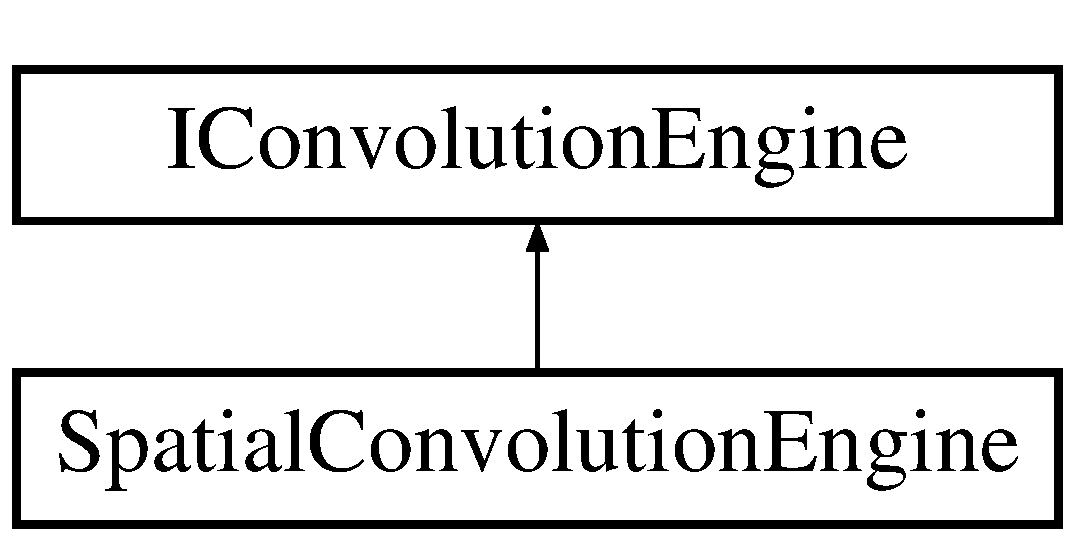
\includegraphics[height=2.000000cm]{class_spatial_convolution_engine}
\end{center}
\end{figure}
\subsection*{Public Member Functions}
\begin{DoxyCompactItemize}
\item 
\hyperlink{class_spatial_convolution_engine_a934e9613ba487297befd6e064bbd5d7a}{Spatial\-Convolution\-Engine} (int type, size\-\_\-t flen)
\item 
virtual \hyperlink{class_spatial_convolution_engine_a07b28be0c28a1c47bc6f2a7459155802}{$\sim$\-Spatial\-Convolution\-Engine} ()
\item 
virtual void \hyperlink{class_spatial_convolution_engine_ad27aad7b65dfa3ec6a617eed96c01d9c}{set\-Filters} (const \hyperlink{types_8hpp_a3207a7addcfa415d1c83622febcb1e9b}{vector\-Mat} \&filters)
\begin{DoxyCompactList}\small\item\em set the filters \end{DoxyCompactList}\item 
virtual void \hyperlink{class_spatial_convolution_engine_a6db3b5e9428ee74e1b4e9e7f7111cad5}{pdf} (const \hyperlink{types_8hpp_a3207a7addcfa415d1c83622febcb1e9b}{vector\-Mat} \&features, \hyperlink{types_8hpp_a33cacb85be7b8df3dc0b67d5d849f4cc}{vector2\-D\-Mat} \&responses)
\begin{DoxyCompactList}\small\item\em Calculate the responses of a set of features to a set of filter experts. \end{DoxyCompactList}\end{DoxyCompactItemize}
\subsection*{Private Member Functions}
\begin{DoxyCompactItemize}
\item 
void \hyperlink{class_spatial_convolution_engine_a3c31cd8797e4c99ccf68dfa558319750}{convolve} (const cv\-::\-Mat \&feature, \hyperlink{types_8hpp_a429d786862fa9bc087b66651599c66dd}{vector\-Filter\-Engine} \&filter, cv\-::\-Mat \&\hyperlink{class_spatial_convolution_engine_a6db3b5e9428ee74e1b4e9e7f7111cad5}{pdf}, const size\-\_\-t stride)
\begin{DoxyCompactList}\small\item\em Convolve two matrices, with a stride of greater than one. \end{DoxyCompactList}\end{DoxyCompactItemize}
\subsection*{Private Attributes}
\begin{DoxyCompactItemize}
\item 
int \hyperlink{class_spatial_convolution_engine_a913adab567840b6d1b2407c3b22ca108}{type\-\_\-}
\begin{DoxyCompactList}\small\item\em the internally supported convolution type, taken from the filter type \end{DoxyCompactList}\item 
size\-\_\-t \hyperlink{class_spatial_convolution_engine_a5d58b30ec6846ef7ccf98f980d4fc957}{flen\-\_\-}
\begin{DoxyCompactList}\small\item\em the number of layers to each filter \end{DoxyCompactList}\item 
\hyperlink{types_8hpp_a3ce0f1abc3fabcd40ad0ea8621d0d552}{vector2\-D\-Filter\-Engine} \hyperlink{class_spatial_convolution_engine_aec615ebfbedc8b7812481be1c2bcb1e5}{filters\-\_\-}
\begin{DoxyCompactList}\small\item\em the internal representation of the filters \end{DoxyCompactList}\end{DoxyCompactItemize}


\subsection{Constructor \& Destructor Documentation}
\hypertarget{class_spatial_convolution_engine_a934e9613ba487297befd6e064bbd5d7a}{\index{Spatial\-Convolution\-Engine@{Spatial\-Convolution\-Engine}!Spatial\-Convolution\-Engine@{Spatial\-Convolution\-Engine}}
\index{Spatial\-Convolution\-Engine@{Spatial\-Convolution\-Engine}!SpatialConvolutionEngine@{Spatial\-Convolution\-Engine}}
\subsubsection[{Spatial\-Convolution\-Engine}]{\setlength{\rightskip}{0pt plus 5cm}Spatial\-Convolution\-Engine\-::\-Spatial\-Convolution\-Engine (
\begin{DoxyParamCaption}
\item[{int}]{type, }
\item[{size\-\_\-t}]{flen}
\end{DoxyParamCaption}
)}}\label{class_spatial_convolution_engine_a934e9613ba487297befd6e064bbd5d7a}
\hypertarget{class_spatial_convolution_engine_a07b28be0c28a1c47bc6f2a7459155802}{\index{Spatial\-Convolution\-Engine@{Spatial\-Convolution\-Engine}!$\sim$\-Spatial\-Convolution\-Engine@{$\sim$\-Spatial\-Convolution\-Engine}}
\index{$\sim$\-Spatial\-Convolution\-Engine@{$\sim$\-Spatial\-Convolution\-Engine}!SpatialConvolutionEngine@{Spatial\-Convolution\-Engine}}
\subsubsection[{$\sim$\-Spatial\-Convolution\-Engine}]{\setlength{\rightskip}{0pt plus 5cm}Spatial\-Convolution\-Engine\-::$\sim$\-Spatial\-Convolution\-Engine (
\begin{DoxyParamCaption}
{}
\end{DoxyParamCaption}
)\hspace{0.3cm}{\ttfamily [virtual]}}}\label{class_spatial_convolution_engine_a07b28be0c28a1c47bc6f2a7459155802}


\subsection{Member Function Documentation}
\hypertarget{class_spatial_convolution_engine_a3c31cd8797e4c99ccf68dfa558319750}{\index{Spatial\-Convolution\-Engine@{Spatial\-Convolution\-Engine}!convolve@{convolve}}
\index{convolve@{convolve}!SpatialConvolutionEngine@{Spatial\-Convolution\-Engine}}
\subsubsection[{convolve}]{\setlength{\rightskip}{0pt plus 5cm}void Spatial\-Convolution\-Engine\-::convolve (
\begin{DoxyParamCaption}
\item[{const cv\-::\-Mat \&}]{feature, }
\item[{{\bf vector\-Filter\-Engine} \&}]{filter, }
\item[{cv\-::\-Mat \&}]{pdf, }
\item[{const size\-\_\-t}]{stride}
\end{DoxyParamCaption}
)\hspace{0.3cm}{\ttfamily [private]}}}\label{class_spatial_convolution_engine_a3c31cd8797e4c99ccf68dfa558319750}


Convolve two matrices, with a stride of greater than one. 

This is a specialized 2\-D convolution algorithm with a stride of greater than one. It is designed to convolve a filter with a feature, where at each pixel an S\-V\-M must be evaluated (leading to a stride of S\-V\-M weight length). The convolution can be thought of as flattened a 2.\-5\-D convolution where the (i,j) dimension is the spatial plane and the (k) dimension is the S\-V\-M weights of the pixels.

The function supports multithreading via Open\-M\-P


\begin{DoxyParams}{Parameters}
{\em feature} & the feature matrix \\
\hline
{\em filter} & the filter (S\-V\-M) \\
\hline
{\em pdf} & the response to return \\
\hline
{\em stride} & the S\-V\-M weight length \\
\hline
\end{DoxyParams}
\hypertarget{class_spatial_convolution_engine_a6db3b5e9428ee74e1b4e9e7f7111cad5}{\index{Spatial\-Convolution\-Engine@{Spatial\-Convolution\-Engine}!pdf@{pdf}}
\index{pdf@{pdf}!SpatialConvolutionEngine@{Spatial\-Convolution\-Engine}}
\subsubsection[{pdf}]{\setlength{\rightskip}{0pt plus 5cm}void Spatial\-Convolution\-Engine\-::pdf (
\begin{DoxyParamCaption}
\item[{const {\bf vector\-Mat} \&}]{features, }
\item[{{\bf vector2\-D\-Mat} \&}]{responses}
\end{DoxyParamCaption}
)\hspace{0.3cm}{\ttfamily [virtual]}}}\label{class_spatial_convolution_engine_a6db3b5e9428ee74e1b4e9e7f7111cad5}


Calculate the responses of a set of features to a set of filter experts. 

A response represents the likelihood of the part appearing at each location of the feature map. \hyperlink{class_parts}{Parts} are support vector machines (S\-V\-Ms) represented as filters. The convolution of a filter with a feature produces a probability density function (pdf) of part location 
\begin{DoxyParams}{Parameters}
{\em features} & the input features (at different scales, and by extension, size) \\
\hline
{\em responses} & the vector of responses (pdfs) to return \\
\hline
\end{DoxyParams}


Implements \hyperlink{class_i_convolution_engine_ab5aaabb634629a714d397a6c1a9c9400}{I\-Convolution\-Engine}.

\hypertarget{class_spatial_convolution_engine_ad27aad7b65dfa3ec6a617eed96c01d9c}{\index{Spatial\-Convolution\-Engine@{Spatial\-Convolution\-Engine}!set\-Filters@{set\-Filters}}
\index{set\-Filters@{set\-Filters}!SpatialConvolutionEngine@{Spatial\-Convolution\-Engine}}
\subsubsection[{set\-Filters}]{\setlength{\rightskip}{0pt plus 5cm}void Spatial\-Convolution\-Engine\-::set\-Filters (
\begin{DoxyParamCaption}
\item[{const {\bf vector\-Mat} \&}]{filters}
\end{DoxyParamCaption}
)\hspace{0.3cm}{\ttfamily [virtual]}}}\label{class_spatial_convolution_engine_ad27aad7b65dfa3ec6a617eed96c01d9c}


set the filters 

given a set of filters, split each filter channel into a plane, in preparation for convolution


\begin{DoxyParams}{Parameters}
{\em filters} & the filters \\
\hline
\end{DoxyParams}


Implements \hyperlink{class_i_convolution_engine_a3570aae351b5fcb93bcd87a06c65ea0a}{I\-Convolution\-Engine}.



\subsection{Field Documentation}
\hypertarget{class_spatial_convolution_engine_aec615ebfbedc8b7812481be1c2bcb1e5}{\index{Spatial\-Convolution\-Engine@{Spatial\-Convolution\-Engine}!filters\-\_\-@{filters\-\_\-}}
\index{filters\-\_\-@{filters\-\_\-}!SpatialConvolutionEngine@{Spatial\-Convolution\-Engine}}
\subsubsection[{filters\-\_\-}]{\setlength{\rightskip}{0pt plus 5cm}{\bf vector2\-D\-Filter\-Engine} Spatial\-Convolution\-Engine\-::filters\-\_\-\hspace{0.3cm}{\ttfamily [private]}}}\label{class_spatial_convolution_engine_aec615ebfbedc8b7812481be1c2bcb1e5}


the internal representation of the filters 

\hypertarget{class_spatial_convolution_engine_a5d58b30ec6846ef7ccf98f980d4fc957}{\index{Spatial\-Convolution\-Engine@{Spatial\-Convolution\-Engine}!flen\-\_\-@{flen\-\_\-}}
\index{flen\-\_\-@{flen\-\_\-}!SpatialConvolutionEngine@{Spatial\-Convolution\-Engine}}
\subsubsection[{flen\-\_\-}]{\setlength{\rightskip}{0pt plus 5cm}size\-\_\-t Spatial\-Convolution\-Engine\-::flen\-\_\-\hspace{0.3cm}{\ttfamily [private]}}}\label{class_spatial_convolution_engine_a5d58b30ec6846ef7ccf98f980d4fc957}


the number of layers to each filter 

\hypertarget{class_spatial_convolution_engine_a913adab567840b6d1b2407c3b22ca108}{\index{Spatial\-Convolution\-Engine@{Spatial\-Convolution\-Engine}!type\-\_\-@{type\-\_\-}}
\index{type\-\_\-@{type\-\_\-}!SpatialConvolutionEngine@{Spatial\-Convolution\-Engine}}
\subsubsection[{type\-\_\-}]{\setlength{\rightskip}{0pt plus 5cm}int Spatial\-Convolution\-Engine\-::type\-\_\-\hspace{0.3cm}{\ttfamily [private]}}}\label{class_spatial_convolution_engine_a913adab567840b6d1b2407c3b22ca108}


the internally supported convolution type, taken from the filter type 



The documentation for this class was generated from the following files\-:\begin{DoxyCompactItemize}
\item 
/\-Users/m29474/\-Desktop/code/openbr/3rdparty/\-Parts\-Based\-Detector/include/\hyperlink{_spatial_convolution_engine_8hpp}{Spatial\-Convolution\-Engine.\-hpp}\item 
/\-Users/m29474/\-Desktop/code/openbr/3rdparty/\-Parts\-Based\-Detector/src/\hyperlink{_spatial_convolution_engine_8cpp}{Spatial\-Convolution\-Engine.\-cpp}\end{DoxyCompactItemize}

\hypertarget{class_stereo_camera_model}{\section{Stereo\-Camera\-Model Class Reference}
\label{class_stereo_camera_model}\index{Stereo\-Camera\-Model@{Stereo\-Camera\-Model}}
}


Slim implementation of camera model for non-\/\-R\-O\-S users.  




{\ttfamily \#include $<$Stereo\-Camera\-Model.\-hpp$>$}

\subsection*{Public Member Functions}
\begin{DoxyCompactItemize}
\item 
\hyperlink{class_stereo_camera_model_a2da893a6e95cc9e7bf3218b74706fd60}{Stereo\-Camera\-Model} ()
\item 
virtual \hyperlink{class_stereo_camera_model_afe05ff04fb566a2097afa236a95e39a2}{$\sim$\-Stereo\-Camera\-Model} ()
\end{DoxyCompactItemize}


\subsection{Detailed Description}
Slim implementation of camera model for non-\/\-R\-O\-S users. 

\subsection{Constructor \& Destructor Documentation}
\hypertarget{class_stereo_camera_model_a2da893a6e95cc9e7bf3218b74706fd60}{\index{Stereo\-Camera\-Model@{Stereo\-Camera\-Model}!Stereo\-Camera\-Model@{Stereo\-Camera\-Model}}
\index{Stereo\-Camera\-Model@{Stereo\-Camera\-Model}!StereoCameraModel@{Stereo\-Camera\-Model}}
\subsubsection[{Stereo\-Camera\-Model}]{\setlength{\rightskip}{0pt plus 5cm}Stereo\-Camera\-Model\-::\-Stereo\-Camera\-Model (
\begin{DoxyParamCaption}
{}
\end{DoxyParamCaption}
)}}\label{class_stereo_camera_model_a2da893a6e95cc9e7bf3218b74706fd60}
\hypertarget{class_stereo_camera_model_afe05ff04fb566a2097afa236a95e39a2}{\index{Stereo\-Camera\-Model@{Stereo\-Camera\-Model}!$\sim$\-Stereo\-Camera\-Model@{$\sim$\-Stereo\-Camera\-Model}}
\index{$\sim$\-Stereo\-Camera\-Model@{$\sim$\-Stereo\-Camera\-Model}!StereoCameraModel@{Stereo\-Camera\-Model}}
\subsubsection[{$\sim$\-Stereo\-Camera\-Model}]{\setlength{\rightskip}{0pt plus 5cm}Stereo\-Camera\-Model\-::$\sim$\-Stereo\-Camera\-Model (
\begin{DoxyParamCaption}
{}
\end{DoxyParamCaption}
)\hspace{0.3cm}{\ttfamily [virtual]}}}\label{class_stereo_camera_model_afe05ff04fb566a2097afa236a95e39a2}


The documentation for this class was generated from the following files\-:\begin{DoxyCompactItemize}
\item 
/\-Users/m29474/\-Desktop/code/openbr/3rdparty/\-Parts\-Based\-Detector/include/\hyperlink{_stereo_camera_model_8hpp}{Stereo\-Camera\-Model.\-hpp}\item 
/\-Users/m29474/\-Desktop/code/openbr/3rdparty/\-Parts\-Based\-Detector/src/\hyperlink{_stereo_camera_model_8cpp}{Stereo\-Camera\-Model.\-cpp}\end{DoxyCompactItemize}

\hypertarget{class_visualize}{\section{Visualize Class Reference}
\label{class_visualize}\index{Visualize@{Visualize}}
}


visualize detection candidates  




{\ttfamily \#include $<$Visualize.\-hpp$>$}

\subsection*{Public Member Functions}
\begin{DoxyCompactItemize}
\item 
\hyperlink{class_visualize_a8d4163ad53518ec0c8a3eaec2bf2fe7b}{Visualize} ()
\item 
\hyperlink{class_visualize_aa4934674b915dc27dd262c5b5a6970b0}{Visualize} (std\-::string name)
\item 
virtual \hyperlink{class_visualize_a50a487bde1d6e77a2b16a2abb28dd066}{$\sim$\-Visualize} ()
\item 
void \hyperlink{class_visualize_ada4023e56a4a59e9b8ecd6c1d8c4c99b}{candidates} (const cv\-::\-Mat \&im, const \hyperlink{types_8hpp_a04eefdf70d6c6b8effb5170271f1db05}{vector\-Candidate} \&candidates, cv\-::\-Mat \&canvas, bool display\-\_\-confidence=false) const 
\item 
void \hyperlink{class_visualize_a6a24ad950e8e20d89a908cf87b709a94}{candidates} (const cv\-::\-Mat \&im, const \hyperlink{types_8hpp_a04eefdf70d6c6b8effb5170271f1db05}{vector\-Candidate} \&candidates, size\-\_\-t N, cv\-::\-Mat \&canvas, bool display\-\_\-confidence=false) const 
\item 
void \hyperlink{class_visualize_a49be21958241fe18358d999483d734e2}{candidates} (const cv\-::\-Mat \&im, const \hyperlink{class_candidate}{Candidate} \&candidate, cv\-::\-Mat \&canvas, bool display\-\_\-confidence=true) const 
\item 
void \hyperlink{class_visualize_a0464561197342e3a26d2f2bf317f3611}{image} (const cv\-::\-Mat \&im) const 
\begin{DoxyCompactList}\small\item\em display the raw image with no overlay \end{DoxyCompactList}\end{DoxyCompactItemize}
\subsection*{Private Attributes}
\begin{DoxyCompactItemize}
\item 
std\-::string \hyperlink{class_visualize_a1407427a175d3a6098df7c300c27bd0d}{name\-\_\-}
\begin{DoxyCompactList}\small\item\em the name of the Open\-C\-V window \end{DoxyCompactList}\end{DoxyCompactItemize}


\subsection{Detailed Description}
visualize detection candidates 

visualize a collection of object detection candidates by rendering the input image to screen, and overlaying the detection bounding boxes of each of the parts, with optional confidence values 

\subsection{Constructor \& Destructor Documentation}
\hypertarget{class_visualize_a8d4163ad53518ec0c8a3eaec2bf2fe7b}{\index{Visualize@{Visualize}!Visualize@{Visualize}}
\index{Visualize@{Visualize}!Visualize@{Visualize}}
\subsubsection[{Visualize}]{\setlength{\rightskip}{0pt plus 5cm}Visualize\-::\-Visualize (
\begin{DoxyParamCaption}
{}
\end{DoxyParamCaption}
)\hspace{0.3cm}{\ttfamily [inline]}}}\label{class_visualize_a8d4163ad53518ec0c8a3eaec2bf2fe7b}
\hypertarget{class_visualize_aa4934674b915dc27dd262c5b5a6970b0}{\index{Visualize@{Visualize}!Visualize@{Visualize}}
\index{Visualize@{Visualize}!Visualize@{Visualize}}
\subsubsection[{Visualize}]{\setlength{\rightskip}{0pt plus 5cm}Visualize\-::\-Visualize (
\begin{DoxyParamCaption}
\item[{std\-::string}]{name}
\end{DoxyParamCaption}
)\hspace{0.3cm}{\ttfamily [inline]}}}\label{class_visualize_aa4934674b915dc27dd262c5b5a6970b0}
\hypertarget{class_visualize_a50a487bde1d6e77a2b16a2abb28dd066}{\index{Visualize@{Visualize}!$\sim$\-Visualize@{$\sim$\-Visualize}}
\index{$\sim$\-Visualize@{$\sim$\-Visualize}!Visualize@{Visualize}}
\subsubsection[{$\sim$\-Visualize}]{\setlength{\rightskip}{0pt plus 5cm}virtual Visualize\-::$\sim$\-Visualize (
\begin{DoxyParamCaption}
{}
\end{DoxyParamCaption}
)\hspace{0.3cm}{\ttfamily [inline]}, {\ttfamily [virtual]}}}\label{class_visualize_a50a487bde1d6e77a2b16a2abb28dd066}


\subsection{Member Function Documentation}
\hypertarget{class_visualize_ada4023e56a4a59e9b8ecd6c1d8c4c99b}{\index{Visualize@{Visualize}!candidates@{candidates}}
\index{candidates@{candidates}!Visualize@{Visualize}}
\subsubsection[{candidates}]{\setlength{\rightskip}{0pt plus 5cm}void Visualize\-::candidates (
\begin{DoxyParamCaption}
\item[{const cv\-::\-Mat \&}]{im, }
\item[{const {\bf vector\-Candidate} \&}]{candidates, }
\item[{cv\-::\-Mat \&}]{canvas, }
\item[{bool}]{display\-\_\-confidence = {\ttfamily false}}
\end{DoxyParamCaption}
) const}}\label{class_visualize_ada4023e56a4a59e9b8ecd6c1d8c4c99b}
\hypertarget{class_visualize_a6a24ad950e8e20d89a908cf87b709a94}{\index{Visualize@{Visualize}!candidates@{candidates}}
\index{candidates@{candidates}!Visualize@{Visualize}}
\subsubsection[{candidates}]{\setlength{\rightskip}{0pt plus 5cm}void Visualize\-::candidates (
\begin{DoxyParamCaption}
\item[{const cv\-::\-Mat \&}]{im, }
\item[{const {\bf vector\-Candidate} \&}]{candidates, }
\item[{size\-\_\-t}]{N, }
\item[{cv\-::\-Mat \&}]{canvas, }
\item[{bool}]{display\-\_\-confidence = {\ttfamily false}}
\end{DoxyParamCaption}
) const}}\label{class_visualize_a6a24ad950e8e20d89a908cf87b709a94}
\hypertarget{class_visualize_a49be21958241fe18358d999483d734e2}{\index{Visualize@{Visualize}!candidates@{candidates}}
\index{candidates@{candidates}!Visualize@{Visualize}}
\subsubsection[{candidates}]{\setlength{\rightskip}{0pt plus 5cm}void Visualize\-::candidates (
\begin{DoxyParamCaption}
\item[{const cv\-::\-Mat \&}]{im, }
\item[{const {\bf Candidate} \&}]{candidate, }
\item[{cv\-::\-Mat \&}]{canvas, }
\item[{bool}]{display\-\_\-confidence = {\ttfamily true}}
\end{DoxyParamCaption}
) const}}\label{class_visualize_a49be21958241fe18358d999483d734e2}
\hypertarget{class_visualize_a0464561197342e3a26d2f2bf317f3611}{\index{Visualize@{Visualize}!image@{image}}
\index{image@{image}!Visualize@{Visualize}}
\subsubsection[{image}]{\setlength{\rightskip}{0pt plus 5cm}void Visualize\-::image (
\begin{DoxyParamCaption}
\item[{const cv\-::\-Mat \&}]{im}
\end{DoxyParamCaption}
) const}}\label{class_visualize_a0464561197342e3a26d2f2bf317f3611}


display the raw image with no overlay 


\begin{DoxyParams}{Parameters}
{\em im} & the input image frame \\
\hline
\end{DoxyParams}


\subsection{Field Documentation}
\hypertarget{class_visualize_a1407427a175d3a6098df7c300c27bd0d}{\index{Visualize@{Visualize}!name\-\_\-@{name\-\_\-}}
\index{name\-\_\-@{name\-\_\-}!Visualize@{Visualize}}
\subsubsection[{name\-\_\-}]{\setlength{\rightskip}{0pt plus 5cm}std\-::string Visualize\-::name\-\_\-\hspace{0.3cm}{\ttfamily [private]}}}\label{class_visualize_a1407427a175d3a6098df7c300c27bd0d}


the name of the Open\-C\-V window 



The documentation for this class was generated from the following files\-:\begin{DoxyCompactItemize}
\item 
/\-Users/m29474/\-Desktop/code/openbr/3rdparty/\-Parts\-Based\-Detector/include/\hyperlink{_visualize_8hpp}{Visualize.\-hpp}\item 
/\-Users/m29474/\-Desktop/code/openbr/3rdparty/\-Parts\-Based\-Detector/src/\hyperlink{_visualize_8cpp}{Visualize.\-cpp}\end{DoxyCompactItemize}

\chapter{File Documentation}
\hypertarget{_candidate_8hpp}{\section{/\-Users/m29474/\-Desktop/code/openbr/3rdparty/\-Parts\-Based\-Detector/include/\-Candidate.hpp File Reference}
\label{_candidate_8hpp}\index{/\-Users/m29474/\-Desktop/code/openbr/3rdparty/\-Parts\-Based\-Detector/include/\-Candidate.\-hpp@{/\-Users/m29474/\-Desktop/code/openbr/3rdparty/\-Parts\-Based\-Detector/include/\-Candidate.\-hpp}}
}
{\ttfamily \#include $<$algorithm$>$}\\*
{\ttfamily \#include $<$iostream$>$}\\*
{\ttfamily \#include $<$limits$>$}\\*
{\ttfamily \#include $<$opencv2/core/core.\-hpp$>$}\\*
{\ttfamily \#include \char`\"{}types.\-hpp\char`\"{}}\\*
{\ttfamily \#include \char`\"{}Rect3.\-hpp\char`\"{}}\\*
{\ttfamily \#include \char`\"{}Math.\-hpp\char`\"{}}\\*
\subsection*{Data Structures}
\begin{DoxyCompactItemize}
\item 
class \hyperlink{class_candidate}{Candidate}
\begin{DoxyCompactList}\small\item\em detection candidate \end{DoxyCompactList}\end{DoxyCompactItemize}

\hypertarget{_depth_consistency_8hpp}{\section{/\-Users/m29474/\-Desktop/code/openbr/3rdparty/\-Parts\-Based\-Detector/include/\-Depth\-Consistency.hpp File Reference}
\label{_depth_consistency_8hpp}\index{/\-Users/m29474/\-Desktop/code/openbr/3rdparty/\-Parts\-Based\-Detector/include/\-Depth\-Consistency.\-hpp@{/\-Users/m29474/\-Desktop/code/openbr/3rdparty/\-Parts\-Based\-Detector/include/\-Depth\-Consistency.\-hpp}}
}
{\ttfamily \#include $<$vector$>$}\\*
{\ttfamily \#include $<$opencv2/core/core.\-hpp$>$}\\*
{\ttfamily \#include \char`\"{}Stereo\-Camera\-Model.\-hpp\char`\"{}}\\*
{\ttfamily \#include \char`\"{}types.\-hpp\char`\"{}}\\*
\subsection*{Data Structures}
\begin{DoxyCompactItemize}
\item 
class \hyperlink{class_depth_consistency}{Depth\-Consistency}
\begin{DoxyCompactList}\small\item\em Search space pruning via depth consistency. \end{DoxyCompactList}\end{DoxyCompactItemize}

\hypertarget{_distance_transform_8hpp}{\section{/\-Users/m29474/\-Desktop/code/openbr/3rdparty/\-Parts\-Based\-Detector/include/\-Distance\-Transform.hpp File Reference}
\label{_distance_transform_8hpp}\index{/\-Users/m29474/\-Desktop/code/openbr/3rdparty/\-Parts\-Based\-Detector/include/\-Distance\-Transform.\-hpp@{/\-Users/m29474/\-Desktop/code/openbr/3rdparty/\-Parts\-Based\-Detector/include/\-Distance\-Transform.\-hpp}}
}
{\ttfamily \#include $<$limits$>$}\\*
{\ttfamily \#include $<$opencv2/core/core.\-hpp$>$}\\*
\subsection*{Data Structures}
\begin{DoxyCompactItemize}
\item 
class \hyperlink{class_penalty_function}{Penalty\-Function}
\begin{DoxyCompactList}\small\item\em an interface for penalty functions to be passed to \hyperlink{class_distance_transform}{Distance\-Transform} \end{DoxyCompactList}\item 
class \hyperlink{class_quadratic}{Quadratic}
\begin{DoxyCompactList}\small\item\em quadratic penalty function \end{DoxyCompactList}\item 
class \hyperlink{class_distance_transform}{Distance\-Transform$<$ T $>$}
\begin{DoxyCompactList}\small\item\em class for performing distance transforms of sampled functions \end{DoxyCompactList}\end{DoxyCompactItemize}

\hypertarget{_dynamic_program_8hpp}{\section{/\-Users/m29474/\-Desktop/code/openbr/3rdparty/\-Parts\-Based\-Detector/include/\-Dynamic\-Program.hpp File Reference}
\label{_dynamic_program_8hpp}\index{/\-Users/m29474/\-Desktop/code/openbr/3rdparty/\-Parts\-Based\-Detector/include/\-Dynamic\-Program.\-hpp@{/\-Users/m29474/\-Desktop/code/openbr/3rdparty/\-Parts\-Based\-Detector/include/\-Dynamic\-Program.\-hpp}}
}
{\ttfamily \#include $<$vector$>$}\\*
{\ttfamily \#include $<$opencv2/core/core.\-hpp$>$}\\*
{\ttfamily \#include \char`\"{}Candidate.\-hpp\char`\"{}}\\*
{\ttfamily \#include \char`\"{}Distance\-Transform.\-hpp\char`\"{}}\\*
{\ttfamily \#include \char`\"{}Model.\-hpp\char`\"{}}\\*
{\ttfamily \#include \char`\"{}Parts.\-hpp\char`\"{}}\\*
{\ttfamily \#include \char`\"{}types.\-hpp\char`\"{}}\\*
\subsection*{Data Structures}
\begin{DoxyCompactItemize}
\item 
class \hyperlink{class_dynamic_program}{Dynamic\-Program$<$ T $>$}
\begin{DoxyCompactList}\small\item\em Dynamic Program to calculate the best holistic detection. \end{DoxyCompactList}\end{DoxyCompactItemize}

\hypertarget{_file_storage_model_8hpp}{\section{/\-Users/m29474/\-Desktop/code/openbr/3rdparty/\-Parts\-Based\-Detector/include/\-File\-Storage\-Model.hpp File Reference}
\label{_file_storage_model_8hpp}\index{/\-Users/m29474/\-Desktop/code/openbr/3rdparty/\-Parts\-Based\-Detector/include/\-File\-Storage\-Model.\-hpp@{/\-Users/m29474/\-Desktop/code/openbr/3rdparty/\-Parts\-Based\-Detector/include/\-File\-Storage\-Model.\-hpp}}
}
{\ttfamily \#include $<$sstream$>$}\\*
{\ttfamily \#include \char`\"{}Model.\-hpp\char`\"{}}\\*
\subsection*{Data Structures}
\begin{DoxyCompactItemize}
\item 
class \hyperlink{class_file_storage_model}{File\-Storage\-Model}
\begin{DoxyCompactList}\small\item\em \hyperlink{class_model}{Model} with cv\-::\-File\-Storage (de-\/)serialization. \end{DoxyCompactList}\end{DoxyCompactItemize}

\hypertarget{_fourier_convolution_engine_8hpp}{\section{/\-Users/m29474/\-Desktop/code/openbr/3rdparty/\-Parts\-Based\-Detector/include/\-Fourier\-Convolution\-Engine.hpp File Reference}
\label{_fourier_convolution_engine_8hpp}\index{/\-Users/m29474/\-Desktop/code/openbr/3rdparty/\-Parts\-Based\-Detector/include/\-Fourier\-Convolution\-Engine.\-hpp@{/\-Users/m29474/\-Desktop/code/openbr/3rdparty/\-Parts\-Based\-Detector/include/\-Fourier\-Convolution\-Engine.\-hpp}}
}
{\ttfamily \#include \char`\"{}I\-Convolution\-Engine.\-hpp\char`\"{}}\\*
\subsection*{Data Structures}
\begin{DoxyCompactItemize}
\item 
class \hyperlink{class_fourier_convolution_engine}{Fourier\-Convolution\-Engine}
\end{DoxyCompactItemize}

\hypertarget{_h_o_g_features_8hpp}{\section{/\-Users/m29474/\-Desktop/code/openbr/3rdparty/\-Parts\-Based\-Detector/include/\-H\-O\-G\-Features.hpp File Reference}
\label{_h_o_g_features_8hpp}\index{/\-Users/m29474/\-Desktop/code/openbr/3rdparty/\-Parts\-Based\-Detector/include/\-H\-O\-G\-Features.\-hpp@{/\-Users/m29474/\-Desktop/code/openbr/3rdparty/\-Parts\-Based\-Detector/include/\-H\-O\-G\-Features.\-hpp}}
}
{\ttfamily \#include $<$vector$>$}\\*
{\ttfamily \#include $<$cstdio$>$}\\*
{\ttfamily \#include $<$opencv2/core/core.\-hpp$>$}\\*
{\ttfamily \#include $<$opencv2/imgproc/imgproc.\-hpp$>$}\\*
{\ttfamily \#include \char`\"{}I\-Features.\-hpp\char`\"{}}\\*
{\ttfamily \#include \char`\"{}types.\-hpp\char`\"{}}\\*
\subsection*{Data Structures}
\begin{DoxyCompactItemize}
\item 
class \hyperlink{class_h_o_g_features}{H\-O\-G\-Features$<$ T $>$}
\begin{DoxyCompactList}\small\item\em Implementation of \hyperlink{class_i_features}{I\-Features} interface using H\-O\-G. \end{DoxyCompactList}\end{DoxyCompactItemize}

\hypertarget{_i_convolution_engine_8hpp}{\section{/\-Users/m29474/\-Desktop/code/openbr/3rdparty/\-Parts\-Based\-Detector/include/\-I\-Convolution\-Engine.hpp File Reference}
\label{_i_convolution_engine_8hpp}\index{/\-Users/m29474/\-Desktop/code/openbr/3rdparty/\-Parts\-Based\-Detector/include/\-I\-Convolution\-Engine.\-hpp@{/\-Users/m29474/\-Desktop/code/openbr/3rdparty/\-Parts\-Based\-Detector/include/\-I\-Convolution\-Engine.\-hpp}}
}
{\ttfamily \#include \char`\"{}types.\-hpp\char`\"{}}\\*
\subsection*{Data Structures}
\begin{DoxyCompactItemize}
\item 
class \hyperlink{class_i_convolution_engine}{I\-Convolution\-Engine}
\end{DoxyCompactItemize}

\hypertarget{_i_features_8hpp}{\section{/\-Users/m29474/\-Desktop/code/openbr/3rdparty/\-Parts\-Based\-Detector/include/\-I\-Features.hpp File Reference}
\label{_i_features_8hpp}\index{/\-Users/m29474/\-Desktop/code/openbr/3rdparty/\-Parts\-Based\-Detector/include/\-I\-Features.\-hpp@{/\-Users/m29474/\-Desktop/code/openbr/3rdparty/\-Parts\-Based\-Detector/include/\-I\-Features.\-hpp}}
}
{\ttfamily \#include $<$vector$>$}\\*
{\ttfamily \#include $<$opencv2/core/core.\-hpp$>$}\\*
{\ttfamily \#include \char`\"{}types.\-hpp\char`\"{}}\\*
\subsection*{Data Structures}
\begin{DoxyCompactItemize}
\item 
class \hyperlink{class_i_features}{I\-Features}
\end{DoxyCompactItemize}

\hypertarget{_math_8hpp}{\section{/\-Users/m29474/\-Desktop/code/openbr/3rdparty/\-Parts\-Based\-Detector/include/\-Math.hpp File Reference}
\label{_math_8hpp}\index{/\-Users/m29474/\-Desktop/code/openbr/3rdparty/\-Parts\-Based\-Detector/include/\-Math.\-hpp@{/\-Users/m29474/\-Desktop/code/openbr/3rdparty/\-Parts\-Based\-Detector/include/\-Math.\-hpp}}
}
{\ttfamily \#include $<$cassert$>$}\\*
{\ttfamily \#include $<$vector$>$}\\*
{\ttfamily \#include $<$opencv2/core/core.\-hpp$>$}\\*
{\ttfamily \#include $<$iostream$>$}\\*
{\ttfamily \#include \char`\"{}types.\-hpp\char`\"{}}\\*
\subsection*{Data Structures}
\begin{DoxyCompactItemize}
\item 
class \hyperlink{class_math}{Math}
\end{DoxyCompactItemize}

\hypertarget{_matlab_i_o_model_8hpp}{\section{/\-Users/m29474/\-Desktop/code/openbr/3rdparty/\-Parts\-Based\-Detector/include/\-Matlab\-I\-O\-Model.hpp File Reference}
\label{_matlab_i_o_model_8hpp}\index{/\-Users/m29474/\-Desktop/code/openbr/3rdparty/\-Parts\-Based\-Detector/include/\-Matlab\-I\-O\-Model.\-hpp@{/\-Users/m29474/\-Desktop/code/openbr/3rdparty/\-Parts\-Based\-Detector/include/\-Matlab\-I\-O\-Model.\-hpp}}
}
{\ttfamily \#include \char`\"{}Model.\-hpp\char`\"{}}\\*
{\ttfamily \#include \char`\"{}types.\-hpp\char`\"{}}\\*
\subsection*{Data Structures}
\begin{DoxyCompactItemize}
\item 
class \hyperlink{class_matlab_i_o_model}{Matlab\-I\-O\-Model}
\begin{DoxyCompactList}\small\item\em \hyperlink{class_model}{Model} implementation with Matlab .Mat file deserialization. \end{DoxyCompactList}\end{DoxyCompactItemize}

\hypertarget{_metrics_8hpp}{\section{/\-Users/m29474/\-Desktop/code/openbr/3rdparty/\-Parts\-Based\-Detector/include/\-Metrics.hpp File Reference}
\label{_metrics_8hpp}\index{/\-Users/m29474/\-Desktop/code/openbr/3rdparty/\-Parts\-Based\-Detector/include/\-Metrics.\-hpp@{/\-Users/m29474/\-Desktop/code/openbr/3rdparty/\-Parts\-Based\-Detector/include/\-Metrics.\-hpp}}
}
{\ttfamily \#include $<$opencv2/core/core.\-hpp$>$}\\*
\subsection*{Data Structures}
\begin{DoxyCompactItemize}
\item 
class \hyperlink{class_metrics}{Metrics}
\end{DoxyCompactItemize}

\hypertarget{_model_8hpp}{\section{/\-Users/m29474/\-Desktop/code/openbr/3rdparty/\-Parts\-Based\-Detector/include/\-Model.hpp File Reference}
\label{_model_8hpp}\index{/\-Users/m29474/\-Desktop/code/openbr/3rdparty/\-Parts\-Based\-Detector/include/\-Model.\-hpp@{/\-Users/m29474/\-Desktop/code/openbr/3rdparty/\-Parts\-Based\-Detector/include/\-Model.\-hpp}}
}
{\ttfamily \#include $<$vector$>$}\\*
{\ttfamily \#include $<$string$>$}\\*
{\ttfamily \#include $<$opencv2/core/core.\-hpp$>$}\\*
{\ttfamily \#include \char`\"{}types.\-hpp\char`\"{}}\\*
\subsection*{Data Structures}
\begin{DoxyCompactItemize}
\item 
class \hyperlink{class_model}{Model}
\begin{DoxyCompactList}\small\item\em Monolithic container class for storing model parameters. \end{DoxyCompactList}\end{DoxyCompactItemize}

\hypertarget{nms_8hpp}{\section{/\-Users/m29474/\-Desktop/code/openbr/3rdparty/\-Parts\-Based\-Detector/include/nms.hpp File Reference}
\label{nms_8hpp}\index{/\-Users/m29474/\-Desktop/code/openbr/3rdparty/\-Parts\-Based\-Detector/include/nms.\-hpp@{/\-Users/m29474/\-Desktop/code/openbr/3rdparty/\-Parts\-Based\-Detector/include/nms.\-hpp}}
}
{\ttfamily \#include $<$opencv2/core/core.\-hpp$>$}\\*
\subsection*{Functions}
\begin{DoxyCompactItemize}
\item 
void \hyperlink{nms_8hpp_a62633ed4c8295e1107775f31e6e40305}{non\-Maxima\-Suppression} (const cv\-::\-Mat \&src, const int sz, cv\-::\-Mat \&dst, const cv\-::\-Mat mask=cv\-::\-Mat())
\end{DoxyCompactItemize}


\subsection{Function Documentation}
\hypertarget{nms_8hpp_a62633ed4c8295e1107775f31e6e40305}{\index{nms.\-hpp@{nms.\-hpp}!non\-Maxima\-Suppression@{non\-Maxima\-Suppression}}
\index{non\-Maxima\-Suppression@{non\-Maxima\-Suppression}!nms.hpp@{nms.\-hpp}}
\subsubsection[{non\-Maxima\-Suppression}]{\setlength{\rightskip}{0pt plus 5cm}void non\-Maxima\-Suppression (
\begin{DoxyParamCaption}
\item[{const cv\-::\-Mat \&}]{src, }
\item[{const int}]{sz, }
\item[{cv\-::\-Mat \&}]{dst, }
\item[{const cv\-::\-Mat}]{mask = {\ttfamily cv\-:\-:Mat()}}
\end{DoxyParamCaption}
)}}\label{nms_8hpp_a62633ed4c8295e1107775f31e6e40305}

\hypertarget{_parts_8hpp}{\section{/\-Users/m29474/\-Desktop/code/openbr/3rdparty/\-Parts\-Based\-Detector/include/\-Parts.hpp File Reference}
\label{_parts_8hpp}\index{/\-Users/m29474/\-Desktop/code/openbr/3rdparty/\-Parts\-Based\-Detector/include/\-Parts.\-hpp@{/\-Users/m29474/\-Desktop/code/openbr/3rdparty/\-Parts\-Based\-Detector/include/\-Parts.\-hpp}}
}
{\ttfamily \#include $<$assert.\-h$>$}\\*
{\ttfamily \#include \char`\"{}types.\-hpp\char`\"{}}\\*
\subsection*{Data Structures}
\begin{DoxyCompactItemize}
\item 
class \hyperlink{class_component_part}{Component\-Part}
\begin{DoxyCompactList}\small\item\em \hyperlink{class_parts}{Parts} tree for a single component of the model. \end{DoxyCompactList}\item 
class \hyperlink{class_parts}{Parts}
\begin{DoxyCompactList}\small\item\em a monolithic collection of part parameters \end{DoxyCompactList}\end{DoxyCompactItemize}

\hypertarget{_parts_based_detector_8hpp}{\section{/\-Users/m29474/\-Desktop/code/openbr/3rdparty/\-Parts\-Based\-Detector/include/\-Parts\-Based\-Detector.hpp File Reference}
\label{_parts_based_detector_8hpp}\index{/\-Users/m29474/\-Desktop/code/openbr/3rdparty/\-Parts\-Based\-Detector/include/\-Parts\-Based\-Detector.\-hpp@{/\-Users/m29474/\-Desktop/code/openbr/3rdparty/\-Parts\-Based\-Detector/include/\-Parts\-Based\-Detector.\-hpp}}
}
{\ttfamily \#include $<$string$>$}\\*
{\ttfamily \#include $<$vector$>$}\\*
{\ttfamily \#include $<$opencv2/core/core.\-hpp$>$}\\*
{\ttfamily \#include $<$boost/scoped\-\_\-ptr.\-hpp$>$}\\*
{\ttfamily \#include \char`\"{}Parts.\-hpp\char`\"{}}\\*
{\ttfamily \#include \char`\"{}Model.\-hpp\char`\"{}}\\*
{\ttfamily \#include \char`\"{}Candidate.\-hpp\char`\"{}}\\*
{\ttfamily \#include \char`\"{}I\-Features.\-hpp\char`\"{}}\\*
{\ttfamily \#include \char`\"{}I\-Convolution\-Engine.\-hpp\char`\"{}}\\*
{\ttfamily \#include \char`\"{}Dynamic\-Program.\-hpp\char`\"{}}\\*
{\ttfamily \#include \char`\"{}Search\-Space\-Pruning.\-hpp\char`\"{}}\\*
\subsection*{Data Structures}
\begin{DoxyCompactItemize}
\item 
class \hyperlink{class_parts_based_detector}{Parts\-Based\-Detector$<$ T $>$}
\begin{DoxyCompactList}\small\item\em The main object detection class \hyperlink{class_parts_based_detector}{Parts\-Based\-Detector} is the main entry point for detecting objects. It has a single method \hyperlink{class_parts_based_detector_a351a499cb2d7ab23d388a34c1c8f38a0}{distribute\-Model()} for setting up the detector parameters from a deserialized model, and a method \hyperlink{class_parts_based_detector_a70c77effade6c39b06ddc0102973a1f8}{detect()} for running the detection pipeline. \end{DoxyCompactList}\end{DoxyCompactItemize}

\hypertarget{_point_cloud_clusterer_8h}{\section{/\-Users/m29474/\-Desktop/code/openbr/3rdparty/\-Parts\-Based\-Detector/include/\-Point\-Cloud\-Clusterer.h File Reference}
\label{_point_cloud_clusterer_8h}\index{/\-Users/m29474/\-Desktop/code/openbr/3rdparty/\-Parts\-Based\-Detector/include/\-Point\-Cloud\-Clusterer.\-h@{/\-Users/m29474/\-Desktop/code/openbr/3rdparty/\-Parts\-Based\-Detector/include/\-Point\-Cloud\-Clusterer.\-h}}
}
{\ttfamily \#include $<$vector$>$}\\*
{\ttfamily \#include $<$opencv2/core/core.\-hpp$>$}\\*
{\ttfamily \#include $<$image\-\_\-geometry/pinhole\-\_\-camera\-\_\-model.\-h$>$}\\*
{\ttfamily \#include $<$pcl/point\-\_\-cloud.\-h$>$}\\*
{\ttfamily \#include $<$pcl/point\-\_\-types.\-h$>$}\\*
{\ttfamily \#include \char`\"{}Candidate.\-hpp\char`\"{}}\\*
{\ttfamily \#include \char`\"{}Rect3.\-hpp\char`\"{}}\\*
{\ttfamily \#include \char`\"{}Point\-Cloud\-Clusterer.\-hpp\char`\"{}}\\*
\subsection*{Data Structures}
\begin{DoxyCompactItemize}
\item 
class \hyperlink{class_point_cloud_clusterer}{Point\-Cloud\-Clusterer$<$ Point\-Type $>$}
\end{DoxyCompactItemize}

\hypertarget{_point_cloud_clusterer_8hpp}{\section{/\-Users/m29474/\-Desktop/code/openbr/3rdparty/\-Parts\-Based\-Detector/include/\-Point\-Cloud\-Clusterer.hpp File Reference}
\label{_point_cloud_clusterer_8hpp}\index{/\-Users/m29474/\-Desktop/code/openbr/3rdparty/\-Parts\-Based\-Detector/include/\-Point\-Cloud\-Clusterer.\-hpp@{/\-Users/m29474/\-Desktop/code/openbr/3rdparty/\-Parts\-Based\-Detector/include/\-Point\-Cloud\-Clusterer.\-hpp}}
}
{\ttfamily \#include \char`\"{}Point\-Cloud\-Clusterer.\-h\char`\"{}}\\*
{\ttfamily \#include $<$vector$>$}\\*
{\ttfamily \#include $<$opencv2/core/core.\-hpp$>$}\\*
{\ttfamily \#include $<$pcl/\-Point\-Indices.\-h$>$}\\*
{\ttfamily \#include $<$pcl/filters/crop\-\_\-box.\-h$>$}\\*
{\ttfamily \#include $<$pcl/filters/extract\-\_\-indices.\-h$>$}\\*
{\ttfamily \#include $<$pcl/features/integral\-\_\-image\-\_\-normal.\-h$>$}\\*
{\ttfamily \#include $<$pcl/segmentation/extract\-\_\-clusters.\-h$>$}\\*
{\ttfamily \#include $<$pcl/segmentation/organized\-\_\-multi\-\_\-plane\-\_\-segmentation.\-h$>$}\\*

\hypertarget{_rect3_8hpp}{\section{/\-Users/m29474/\-Desktop/code/openbr/3rdparty/\-Parts\-Based\-Detector/include/\-Rect3.hpp File Reference}
\label{_rect3_8hpp}\index{/\-Users/m29474/\-Desktop/code/openbr/3rdparty/\-Parts\-Based\-Detector/include/\-Rect3.\-hpp@{/\-Users/m29474/\-Desktop/code/openbr/3rdparty/\-Parts\-Based\-Detector/include/\-Rect3.\-hpp}}
}
{\ttfamily \#include $<$opencv2/core/core.\-hpp$>$}\\*
{\ttfamily \#include $<$vector$>$}\\*
\subsection*{Data Structures}
\begin{DoxyCompactItemize}
\item 
class \hyperlink{class_rect3__}{Rect3\-\_\-$<$ T $>$}
\begin{DoxyCompactList}\small\item\em 3\-D rectangle class This class implements a 3\-D rectangle which provides similar functionality to the Open\-C\-V Rect\-\_\- class, but in 3-\/space \end{DoxyCompactList}\end{DoxyCompactItemize}
\subsection*{Typedefs}
\begin{DoxyCompactItemize}
\item 
typedef \hyperlink{class_rect3__}{Rect3\-\_\-}$<$ int $>$ \hyperlink{_rect3_8hpp_a885cb2c7714c1fb158e1090d5739885b}{Rect3}
\begin{DoxyCompactList}\small\item\em convenient typedef for integer type rectangular prisms \end{DoxyCompactList}\item 
typedef \hyperlink{class_rect3__}{Rect3\-\_\-}$<$ float $>$ \hyperlink{_rect3_8hpp_a6743f930e5761892a2c5444764582ed2}{Rect3f}
\item 
typedef \hyperlink{class_rect3__}{Rect3\-\_\-}$<$ double $>$ \hyperlink{_rect3_8hpp_a05172c5a86161981edfe197f57415582}{Rect3d}
\end{DoxyCompactItemize}


\subsection{Typedef Documentation}
\hypertarget{_rect3_8hpp_a885cb2c7714c1fb158e1090d5739885b}{\index{Rect3.\-hpp@{Rect3.\-hpp}!Rect3@{Rect3}}
\index{Rect3@{Rect3}!Rect3.hpp@{Rect3.\-hpp}}
\subsubsection[{Rect3}]{\setlength{\rightskip}{0pt plus 5cm}typedef {\bf Rect3\-\_\-}$<$int$>$ {\bf Rect3}}}\label{_rect3_8hpp_a885cb2c7714c1fb158e1090d5739885b}


convenient typedef for integer type rectangular prisms 

\hypertarget{_rect3_8hpp_a05172c5a86161981edfe197f57415582}{\index{Rect3.\-hpp@{Rect3.\-hpp}!Rect3d@{Rect3d}}
\index{Rect3d@{Rect3d}!Rect3.hpp@{Rect3.\-hpp}}
\subsubsection[{Rect3d}]{\setlength{\rightskip}{0pt plus 5cm}typedef {\bf Rect3\-\_\-}$<$double$>$ {\bf Rect3d}}}\label{_rect3_8hpp_a05172c5a86161981edfe197f57415582}
\hypertarget{_rect3_8hpp_a6743f930e5761892a2c5444764582ed2}{\index{Rect3.\-hpp@{Rect3.\-hpp}!Rect3f@{Rect3f}}
\index{Rect3f@{Rect3f}!Rect3.hpp@{Rect3.\-hpp}}
\subsubsection[{Rect3f}]{\setlength{\rightskip}{0pt plus 5cm}typedef {\bf Rect3\-\_\-}$<$float$>$ {\bf Rect3f}}}\label{_rect3_8hpp_a6743f930e5761892a2c5444764582ed2}

\hypertarget{_search_space_pruning_8hpp}{\section{/\-Users/m29474/\-Desktop/code/openbr/3rdparty/\-Parts\-Based\-Detector/include/\-Search\-Space\-Pruning.hpp File Reference}
\label{_search_space_pruning_8hpp}\index{/\-Users/m29474/\-Desktop/code/openbr/3rdparty/\-Parts\-Based\-Detector/include/\-Search\-Space\-Pruning.\-hpp@{/\-Users/m29474/\-Desktop/code/openbr/3rdparty/\-Parts\-Based\-Detector/include/\-Search\-Space\-Pruning.\-hpp}}
}
{\ttfamily \#include $<$opencv2/core/core.\-hpp$>$}\\*
{\ttfamily \#include $<$limits$>$}\\*
{\ttfamily \#include \char`\"{}Candidate.\-hpp\char`\"{}}\\*
{\ttfamily \#include \char`\"{}Parts.\-hpp\char`\"{}}\\*
{\ttfamily \#include \char`\"{}types.\-hpp\char`\"{}}\\*
\subsection*{Data Structures}
\begin{DoxyCompactItemize}
\item 
class \hyperlink{class_search_space_pruning}{Search\-Space\-Pruning$<$ T $>$}
\end{DoxyCompactItemize}

\hypertarget{_spatial_convolution_engine_8hpp}{\section{/\-Users/m29474/\-Desktop/code/openbr/3rdparty/\-Parts\-Based\-Detector/include/\-Spatial\-Convolution\-Engine.hpp File Reference}
\label{_spatial_convolution_engine_8hpp}\index{/\-Users/m29474/\-Desktop/code/openbr/3rdparty/\-Parts\-Based\-Detector/include/\-Spatial\-Convolution\-Engine.\-hpp@{/\-Users/m29474/\-Desktop/code/openbr/3rdparty/\-Parts\-Based\-Detector/include/\-Spatial\-Convolution\-Engine.\-hpp}}
}
{\ttfamily \#include \char`\"{}I\-Convolution\-Engine.\-hpp\char`\"{}}\\*
\subsection*{Data Structures}
\begin{DoxyCompactItemize}
\item 
class \hyperlink{class_spatial_convolution_engine}{Spatial\-Convolution\-Engine}
\end{DoxyCompactItemize}

\hypertarget{_stereo_camera_model_8hpp}{\section{/\-Users/m29474/\-Desktop/code/openbr/3rdparty/\-Parts\-Based\-Detector/include/\-Stereo\-Camera\-Model.hpp File Reference}
\label{_stereo_camera_model_8hpp}\index{/\-Users/m29474/\-Desktop/code/openbr/3rdparty/\-Parts\-Based\-Detector/include/\-Stereo\-Camera\-Model.\-hpp@{/\-Users/m29474/\-Desktop/code/openbr/3rdparty/\-Parts\-Based\-Detector/include/\-Stereo\-Camera\-Model.\-hpp}}
}
\subsection*{Data Structures}
\begin{DoxyCompactItemize}
\item 
class \hyperlink{class_stereo_camera_model}{Stereo\-Camera\-Model}
\begin{DoxyCompactList}\small\item\em Slim implementation of camera model for non-\/\-R\-O\-S users. \end{DoxyCompactList}\end{DoxyCompactItemize}

\hypertarget{types_8hpp}{\section{/\-Users/m29474/\-Desktop/code/openbr/3rdparty/\-Parts\-Based\-Detector/include/types.hpp File Reference}
\label{types_8hpp}\index{/\-Users/m29474/\-Desktop/code/openbr/3rdparty/\-Parts\-Based\-Detector/include/types.\-hpp@{/\-Users/m29474/\-Desktop/code/openbr/3rdparty/\-Parts\-Based\-Detector/include/types.\-hpp}}
}
{\ttfamily \#include $<$vector$>$}\\*
{\ttfamily \#include $<$opencv2/core/core.\-hpp$>$}\\*
{\ttfamily \#include $<$opencv2/imgproc/imgproc.\-hpp$>$}\\*
\subsection*{Typedefs}
\begin{DoxyCompactItemize}
\item 
typedef std\-::vector$<$ int $>$ \hyperlink{types_8hpp_a44529587d60e73bf0e689a82e5e70a55}{vectori}
\item 
typedef std\-::vector$<$ float $>$ \hyperlink{types_8hpp_a4da5db3ee9e284f719ef5764dbadffc8}{vectorf}
\item 
typedef std\-::vector$<$ cv\-::\-Mat $>$ \hyperlink{types_8hpp_a3207a7addcfa415d1c83622febcb1e9b}{vector\-Mat}
\item 
typedef std\-::vector$<$ cv\-::\-Point $>$ \hyperlink{types_8hpp_ac468fcf6870d6563ac8fa3669845afcc}{vector\-Point}
\item 
typedef std\-::vector$<$ cv\-::\-Point3i $>$ \hyperlink{types_8hpp_ae43c691df1b6cd5df322ac02d8470cfb}{vector\-Point3}
\item 
typedef std\-::vector$<$ \hyperlink{class_candidate}{Candidate} $>$ \hyperlink{types_8hpp_a04eefdf70d6c6b8effb5170271f1db05}{vector\-Candidate}
\item 
typedef std\-::vector\\*
$<$ Matlab\-I\-O\-Container $>$ \hyperlink{types_8hpp_adf4fd3f47484feba467c5eaa96db6fdb}{vector\-Matlab\-I\-O\-Container}
\item 
typedef std\-::vector$<$ cv\-::\-Ptr\\*
$<$ cv\-::\-Filter\-Engine $>$ $>$ \hyperlink{types_8hpp_a429d786862fa9bc087b66651599c66dd}{vector\-Filter\-Engine}
\item 
typedef std\-::vector$<$ \hyperlink{types_8hpp_a44529587d60e73bf0e689a82e5e70a55}{vectori} $>$ \hyperlink{types_8hpp_a93a5e2cfd40d1ff1f10d8bbf11884c41}{vector2\-Di}
\item 
typedef std\-::vector$<$ \hyperlink{types_8hpp_a4da5db3ee9e284f719ef5764dbadffc8}{vectorf} $>$ \hyperlink{types_8hpp_a94f2d563f3725231a6f684b4dce4f1ef}{vector2\-Df}
\item 
typedef std\-::vector$<$ \hyperlink{types_8hpp_a3207a7addcfa415d1c83622febcb1e9b}{vector\-Mat} $>$ \hyperlink{types_8hpp_a33cacb85be7b8df3dc0b67d5d849f4cc}{vector2\-D\-Mat}
\item 
typedef std\-::vector\\*
$<$ \hyperlink{types_8hpp_adf4fd3f47484feba467c5eaa96db6fdb}{vector\-Matlab\-I\-O\-Container} $>$ \hyperlink{types_8hpp_a1c5aa7c185f1e62163eae62b2342f855}{vector2\-D\-Matlab\-I\-O\-Container}
\item 
typedef std\-::vector\\*
$<$ std\-::vector$<$ cv\-::\-Ptr\\*
$<$ cv\-::\-Filter\-Engine $>$ $>$ $>$ \hyperlink{types_8hpp_a3ce0f1abc3fabcd40ad0ea8621d0d552}{vector2\-D\-Filter\-Engine}
\item 
typedef std\-::vector$<$ \hyperlink{types_8hpp_a93a5e2cfd40d1ff1f10d8bbf11884c41}{vector2\-Di} $>$ \hyperlink{types_8hpp_a1f7c8ad00a53fb2d61b3656da9a6581d}{vector3\-Di}
\item 
typedef std\-::vector$<$ \hyperlink{types_8hpp_a33cacb85be7b8df3dc0b67d5d849f4cc}{vector2\-D\-Mat} $>$ \hyperlink{types_8hpp_aa815fac2e2882eb34307cf4b2c7d8623}{vector3\-D\-Mat}
\item 
typedef std\-::vector$<$ \hyperlink{types_8hpp_aa815fac2e2882eb34307cf4b2c7d8623}{vector3\-D\-Mat} $>$ \hyperlink{types_8hpp_a9c446ceac5aee9d97fb9ee36ad27072f}{vector4\-D\-Mat}
\end{DoxyCompactItemize}


\subsection{Typedef Documentation}
\hypertarget{types_8hpp_a94f2d563f3725231a6f684b4dce4f1ef}{\index{types.\-hpp@{types.\-hpp}!vector2\-Df@{vector2\-Df}}
\index{vector2\-Df@{vector2\-Df}!types.hpp@{types.\-hpp}}
\subsubsection[{vector2\-Df}]{\setlength{\rightskip}{0pt plus 5cm}typedef std\-::vector$<${\bf vectorf}$>$ {\bf vector2\-Df}}}\label{types_8hpp_a94f2d563f3725231a6f684b4dce4f1ef}
\hypertarget{types_8hpp_a3ce0f1abc3fabcd40ad0ea8621d0d552}{\index{types.\-hpp@{types.\-hpp}!vector2\-D\-Filter\-Engine@{vector2\-D\-Filter\-Engine}}
\index{vector2\-D\-Filter\-Engine@{vector2\-D\-Filter\-Engine}!types.hpp@{types.\-hpp}}
\subsubsection[{vector2\-D\-Filter\-Engine}]{\setlength{\rightskip}{0pt plus 5cm}typedef std\-::vector$<$std\-::vector$<$cv\-::\-Ptr$<$cv\-::\-Filter\-Engine$>$ $>$ $>$ {\bf vector2\-D\-Filter\-Engine}}}\label{types_8hpp_a3ce0f1abc3fabcd40ad0ea8621d0d552}
\hypertarget{types_8hpp_a93a5e2cfd40d1ff1f10d8bbf11884c41}{\index{types.\-hpp@{types.\-hpp}!vector2\-Di@{vector2\-Di}}
\index{vector2\-Di@{vector2\-Di}!types.hpp@{types.\-hpp}}
\subsubsection[{vector2\-Di}]{\setlength{\rightskip}{0pt plus 5cm}typedef std\-::vector$<${\bf vectori}$>$ {\bf vector2\-Di}}}\label{types_8hpp_a93a5e2cfd40d1ff1f10d8bbf11884c41}
\hypertarget{types_8hpp_a33cacb85be7b8df3dc0b67d5d849f4cc}{\index{types.\-hpp@{types.\-hpp}!vector2\-D\-Mat@{vector2\-D\-Mat}}
\index{vector2\-D\-Mat@{vector2\-D\-Mat}!types.hpp@{types.\-hpp}}
\subsubsection[{vector2\-D\-Mat}]{\setlength{\rightskip}{0pt plus 5cm}typedef std\-::vector$<${\bf vector\-Mat}$>$ {\bf vector2\-D\-Mat}}}\label{types_8hpp_a33cacb85be7b8df3dc0b67d5d849f4cc}
\hypertarget{types_8hpp_a1c5aa7c185f1e62163eae62b2342f855}{\index{types.\-hpp@{types.\-hpp}!vector2\-D\-Matlab\-I\-O\-Container@{vector2\-D\-Matlab\-I\-O\-Container}}
\index{vector2\-D\-Matlab\-I\-O\-Container@{vector2\-D\-Matlab\-I\-O\-Container}!types.hpp@{types.\-hpp}}
\subsubsection[{vector2\-D\-Matlab\-I\-O\-Container}]{\setlength{\rightskip}{0pt plus 5cm}typedef std\-::vector$<${\bf vector\-Matlab\-I\-O\-Container}$>$ {\bf vector2\-D\-Matlab\-I\-O\-Container}}}\label{types_8hpp_a1c5aa7c185f1e62163eae62b2342f855}
\hypertarget{types_8hpp_a1f7c8ad00a53fb2d61b3656da9a6581d}{\index{types.\-hpp@{types.\-hpp}!vector3\-Di@{vector3\-Di}}
\index{vector3\-Di@{vector3\-Di}!types.hpp@{types.\-hpp}}
\subsubsection[{vector3\-Di}]{\setlength{\rightskip}{0pt plus 5cm}typedef std\-::vector$<${\bf vector2\-Di}$>$ {\bf vector3\-Di}}}\label{types_8hpp_a1f7c8ad00a53fb2d61b3656da9a6581d}
\hypertarget{types_8hpp_aa815fac2e2882eb34307cf4b2c7d8623}{\index{types.\-hpp@{types.\-hpp}!vector3\-D\-Mat@{vector3\-D\-Mat}}
\index{vector3\-D\-Mat@{vector3\-D\-Mat}!types.hpp@{types.\-hpp}}
\subsubsection[{vector3\-D\-Mat}]{\setlength{\rightskip}{0pt plus 5cm}typedef std\-::vector$<${\bf vector2\-D\-Mat}$>$ {\bf vector3\-D\-Mat}}}\label{types_8hpp_aa815fac2e2882eb34307cf4b2c7d8623}
\hypertarget{types_8hpp_a9c446ceac5aee9d97fb9ee36ad27072f}{\index{types.\-hpp@{types.\-hpp}!vector4\-D\-Mat@{vector4\-D\-Mat}}
\index{vector4\-D\-Mat@{vector4\-D\-Mat}!types.hpp@{types.\-hpp}}
\subsubsection[{vector4\-D\-Mat}]{\setlength{\rightskip}{0pt plus 5cm}typedef std\-::vector$<${\bf vector3\-D\-Mat}$>$ {\bf vector4\-D\-Mat}}}\label{types_8hpp_a9c446ceac5aee9d97fb9ee36ad27072f}
\hypertarget{types_8hpp_a04eefdf70d6c6b8effb5170271f1db05}{\index{types.\-hpp@{types.\-hpp}!vector\-Candidate@{vector\-Candidate}}
\index{vector\-Candidate@{vector\-Candidate}!types.hpp@{types.\-hpp}}
\subsubsection[{vector\-Candidate}]{\setlength{\rightskip}{0pt plus 5cm}typedef std\-::vector$<${\bf Candidate}$>$ {\bf vector\-Candidate}}}\label{types_8hpp_a04eefdf70d6c6b8effb5170271f1db05}
\hypertarget{types_8hpp_a4da5db3ee9e284f719ef5764dbadffc8}{\index{types.\-hpp@{types.\-hpp}!vectorf@{vectorf}}
\index{vectorf@{vectorf}!types.hpp@{types.\-hpp}}
\subsubsection[{vectorf}]{\setlength{\rightskip}{0pt plus 5cm}typedef std\-::vector$<$float$>$ {\bf vectorf}}}\label{types_8hpp_a4da5db3ee9e284f719ef5764dbadffc8}
\hypertarget{types_8hpp_a429d786862fa9bc087b66651599c66dd}{\index{types.\-hpp@{types.\-hpp}!vector\-Filter\-Engine@{vector\-Filter\-Engine}}
\index{vector\-Filter\-Engine@{vector\-Filter\-Engine}!types.hpp@{types.\-hpp}}
\subsubsection[{vector\-Filter\-Engine}]{\setlength{\rightskip}{0pt plus 5cm}typedef std\-::vector$<$cv\-::\-Ptr$<$cv\-::\-Filter\-Engine$>$ $>$ {\bf vector\-Filter\-Engine}}}\label{types_8hpp_a429d786862fa9bc087b66651599c66dd}
\hypertarget{types_8hpp_a44529587d60e73bf0e689a82e5e70a55}{\index{types.\-hpp@{types.\-hpp}!vectori@{vectori}}
\index{vectori@{vectori}!types.hpp@{types.\-hpp}}
\subsubsection[{vectori}]{\setlength{\rightskip}{0pt plus 5cm}typedef std\-::vector$<$int$>$ {\bf vectori}}}\label{types_8hpp_a44529587d60e73bf0e689a82e5e70a55}
\hypertarget{types_8hpp_a3207a7addcfa415d1c83622febcb1e9b}{\index{types.\-hpp@{types.\-hpp}!vector\-Mat@{vector\-Mat}}
\index{vector\-Mat@{vector\-Mat}!types.hpp@{types.\-hpp}}
\subsubsection[{vector\-Mat}]{\setlength{\rightskip}{0pt plus 5cm}typedef std\-::vector$<$cv\-::\-Mat$>$ {\bf vector\-Mat}}}\label{types_8hpp_a3207a7addcfa415d1c83622febcb1e9b}
\hypertarget{types_8hpp_adf4fd3f47484feba467c5eaa96db6fdb}{\index{types.\-hpp@{types.\-hpp}!vector\-Matlab\-I\-O\-Container@{vector\-Matlab\-I\-O\-Container}}
\index{vector\-Matlab\-I\-O\-Container@{vector\-Matlab\-I\-O\-Container}!types.hpp@{types.\-hpp}}
\subsubsection[{vector\-Matlab\-I\-O\-Container}]{\setlength{\rightskip}{0pt plus 5cm}typedef std\-::vector$<$Matlab\-I\-O\-Container$>$ {\bf vector\-Matlab\-I\-O\-Container}}}\label{types_8hpp_adf4fd3f47484feba467c5eaa96db6fdb}
\hypertarget{types_8hpp_ac468fcf6870d6563ac8fa3669845afcc}{\index{types.\-hpp@{types.\-hpp}!vector\-Point@{vector\-Point}}
\index{vector\-Point@{vector\-Point}!types.hpp@{types.\-hpp}}
\subsubsection[{vector\-Point}]{\setlength{\rightskip}{0pt plus 5cm}typedef std\-::vector$<$cv\-::\-Point$>$ {\bf vector\-Point}}}\label{types_8hpp_ac468fcf6870d6563ac8fa3669845afcc}
\hypertarget{types_8hpp_ae43c691df1b6cd5df322ac02d8470cfb}{\index{types.\-hpp@{types.\-hpp}!vector\-Point3@{vector\-Point3}}
\index{vector\-Point3@{vector\-Point3}!types.hpp@{types.\-hpp}}
\subsubsection[{vector\-Point3}]{\setlength{\rightskip}{0pt plus 5cm}typedef std\-::vector$<$cv\-::\-Point3i$>$ {\bf vector\-Point3}}}\label{types_8hpp_ae43c691df1b6cd5df322ac02d8470cfb}

\hypertarget{_visualize_8hpp}{\section{/\-Users/m29474/\-Desktop/code/openbr/3rdparty/\-Parts\-Based\-Detector/include/\-Visualize.hpp File Reference}
\label{_visualize_8hpp}\index{/\-Users/m29474/\-Desktop/code/openbr/3rdparty/\-Parts\-Based\-Detector/include/\-Visualize.\-hpp@{/\-Users/m29474/\-Desktop/code/openbr/3rdparty/\-Parts\-Based\-Detector/include/\-Visualize.\-hpp}}
}
{\ttfamily \#include $<$opencv2/core/core.\-hpp$>$}\\*
{\ttfamily \#include $<$opencv2/highgui/highgui.\-hpp$>$}\\*
{\ttfamily \#include $<$string$>$}\\*
{\ttfamily \#include $<$vector$>$}\\*
{\ttfamily \#include \char`\"{}Candidate.\-hpp\char`\"{}}\\*
{\ttfamily \#include \char`\"{}types.\-hpp\char`\"{}}\\*
\subsection*{Data Structures}
\begin{DoxyCompactItemize}
\item 
class \hyperlink{class_visualize}{Visualize}
\begin{DoxyCompactList}\small\item\em visualize detection candidates \end{DoxyCompactList}\end{DoxyCompactItemize}

\hypertarget{demo_8cpp}{\section{/\-Users/m29474/\-Desktop/code/openbr/3rdparty/\-Parts\-Based\-Detector/src/demo.cpp File Reference}
\label{demo_8cpp}\index{/\-Users/m29474/\-Desktop/code/openbr/3rdparty/\-Parts\-Based\-Detector/src/demo.\-cpp@{/\-Users/m29474/\-Desktop/code/openbr/3rdparty/\-Parts\-Based\-Detector/src/demo.\-cpp}}
}
{\ttfamily \#include $<$boost/filesystem.\-hpp$>$}\\*
{\ttfamily \#include \char`\"{}Parts\-Based\-Detector.\-hpp\char`\"{}}\\*
{\ttfamily \#include \char`\"{}Candidate.\-hpp\char`\"{}}\\*
{\ttfamily \#include \char`\"{}File\-Storage\-Model.\-hpp\char`\"{}}\\*
{\ttfamily \#include \char`\"{}Visualize.\-hpp\char`\"{}}\\*
{\ttfamily \#include \char`\"{}types.\-hpp\char`\"{}}\\*
{\ttfamily \#include \char`\"{}nms.\-hpp\char`\"{}}\\*
{\ttfamily \#include \char`\"{}Rect3.\-hpp\char`\"{}}\\*
{\ttfamily \#include \char`\"{}Distance\-Transform.\-hpp\char`\"{}}\\*
\subsection*{Functions}
\begin{DoxyCompactItemize}
\item 
int \hyperlink{demo_8cpp_a3c04138a5bfe5d72780bb7e82a18e627}{main} (int argc, char $\ast$$\ast$argv)
\end{DoxyCompactItemize}


\subsection{Function Documentation}
\hypertarget{demo_8cpp_a3c04138a5bfe5d72780bb7e82a18e627}{\index{demo.\-cpp@{demo.\-cpp}!main@{main}}
\index{main@{main}!demo.cpp@{demo.\-cpp}}
\subsubsection[{main}]{\setlength{\rightskip}{0pt plus 5cm}int main (
\begin{DoxyParamCaption}
\item[{int}]{argc, }
\item[{char $\ast$$\ast$}]{argv}
\end{DoxyParamCaption}
)}}\label{demo_8cpp_a3c04138a5bfe5d72780bb7e82a18e627}

\hypertarget{_depth_consistency_8cpp}{\section{/\-Users/m29474/\-Desktop/code/openbr/3rdparty/\-Parts\-Based\-Detector/src/\-Depth\-Consistency.cpp File Reference}
\label{_depth_consistency_8cpp}\index{/\-Users/m29474/\-Desktop/code/openbr/3rdparty/\-Parts\-Based\-Detector/src/\-Depth\-Consistency.\-cpp@{/\-Users/m29474/\-Desktop/code/openbr/3rdparty/\-Parts\-Based\-Detector/src/\-Depth\-Consistency.\-cpp}}
}
{\ttfamily \#include \char`\"{}Depth\-Consistency.\-hpp\char`\"{}}\\*

\hypertarget{_dynamic_program_8cpp}{\section{/\-Users/m29474/\-Desktop/code/openbr/3rdparty/\-Parts\-Based\-Detector/src/\-Dynamic\-Program.cpp File Reference}
\label{_dynamic_program_8cpp}\index{/\-Users/m29474/\-Desktop/code/openbr/3rdparty/\-Parts\-Based\-Detector/src/\-Dynamic\-Program.\-cpp@{/\-Users/m29474/\-Desktop/code/openbr/3rdparty/\-Parts\-Based\-Detector/src/\-Dynamic\-Program.\-cpp}}
}
{\ttfamily \#include \char`\"{}Math.\-hpp\char`\"{}}\\*
{\ttfamily \#include \char`\"{}Dynamic\-Program.\-hpp\char`\"{}}\\*

\hypertarget{_file_storage_model_8cpp}{\section{/\-Users/m29474/\-Desktop/code/openbr/3rdparty/\-Parts\-Based\-Detector/src/\-File\-Storage\-Model.cpp File Reference}
\label{_file_storage_model_8cpp}\index{/\-Users/m29474/\-Desktop/code/openbr/3rdparty/\-Parts\-Based\-Detector/src/\-File\-Storage\-Model.\-cpp@{/\-Users/m29474/\-Desktop/code/openbr/3rdparty/\-Parts\-Based\-Detector/src/\-File\-Storage\-Model.\-cpp}}
}
{\ttfamily \#include $<$sstream$>$}\\*
{\ttfamily \#include \char`\"{}File\-Storage\-Model.\-hpp\char`\"{}}\\*

\hypertarget{_fourier_convolution_engine_8cpp}{\section{/\-Users/m29474/\-Desktop/code/openbr/3rdparty/\-Parts\-Based\-Detector/src/\-Fourier\-Convolution\-Engine.cpp File Reference}
\label{_fourier_convolution_engine_8cpp}\index{/\-Users/m29474/\-Desktop/code/openbr/3rdparty/\-Parts\-Based\-Detector/src/\-Fourier\-Convolution\-Engine.\-cpp@{/\-Users/m29474/\-Desktop/code/openbr/3rdparty/\-Parts\-Based\-Detector/src/\-Fourier\-Convolution\-Engine.\-cpp}}
}
{\ttfamily \#include $<$math.\-h$>$}\\*
{\ttfamily \#include $<$assert.\-h$>$}\\*
{\ttfamily \#include $<$opencv2/core/core.\-hpp$>$}\\*
{\ttfamily \#include $<$opencv2/imgproc/imgproc.\-hpp$>$}\\*
{\ttfamily \#include \char`\"{}Fourier\-Convolution\-Engine.\-hpp\char`\"{}}\\*

\hypertarget{_h_o_g_features_8cpp}{\section{/\-Users/m29474/\-Desktop/code/openbr/3rdparty/\-Parts\-Based\-Detector/src/\-H\-O\-G\-Features.cpp File Reference}
\label{_h_o_g_features_8cpp}\index{/\-Users/m29474/\-Desktop/code/openbr/3rdparty/\-Parts\-Based\-Detector/src/\-H\-O\-G\-Features.\-cpp@{/\-Users/m29474/\-Desktop/code/openbr/3rdparty/\-Parts\-Based\-Detector/src/\-H\-O\-G\-Features.\-cpp}}
}
{\ttfamily \#include $<$cassert$>$}\\*
{\ttfamily \#include \char`\"{}H\-O\-G\-Features.\-hpp\char`\"{}}\\*
\subsection*{Functions}
\begin{DoxyCompactItemize}
\item 
{\footnotesize template$<$typename T $>$ }\\static T \hyperlink{_h_o_g_features_8cpp_a86643e946252a92f84548159035724c3}{square} (const T \&x)
\end{DoxyCompactItemize}


\subsection{Function Documentation}
\hypertarget{_h_o_g_features_8cpp_a86643e946252a92f84548159035724c3}{\index{H\-O\-G\-Features.\-cpp@{H\-O\-G\-Features.\-cpp}!square@{square}}
\index{square@{square}!HOGFeatures.cpp@{H\-O\-G\-Features.\-cpp}}
\subsubsection[{square}]{\setlength{\rightskip}{0pt plus 5cm}template$<$typename T $>$ static T square (
\begin{DoxyParamCaption}
\item[{const T \&}]{x}
\end{DoxyParamCaption}
)\hspace{0.3cm}{\ttfamily [inline]}, {\ttfamily [static]}}}\label{_h_o_g_features_8cpp_a86643e946252a92f84548159035724c3}

\hypertarget{_matlab_i_o_model_8cpp}{\section{/\-Users/m29474/\-Desktop/code/openbr/3rdparty/\-Parts\-Based\-Detector/src/\-Matlab\-I\-O\-Model.cpp File Reference}
\label{_matlab_i_o_model_8cpp}\index{/\-Users/m29474/\-Desktop/code/openbr/3rdparty/\-Parts\-Based\-Detector/src/\-Matlab\-I\-O\-Model.\-cpp@{/\-Users/m29474/\-Desktop/code/openbr/3rdparty/\-Parts\-Based\-Detector/src/\-Matlab\-I\-O\-Model.\-cpp}}
}
{\ttfamily \#include $<$exception$>$}\\*
{\ttfamily \#include $<$boost/filesystem.\-hpp$>$}\\*
{\ttfamily \#include $<$Matlab\-I\-O.\-hpp$>$}\\*
{\ttfamily \#include \char`\"{}Matlab\-I\-O\-Model.\-hpp\char`\"{}}\\*
\subsection*{Functions}
\begin{DoxyCompactItemize}
\item 
static void \hyperlink{_matlab_i_o_model_8cpp_aaf034531aebdbdb52680006ed30031cf}{zero\-Index} (\hyperlink{types_8hpp_a44529587d60e73bf0e689a82e5e70a55}{vectori} \&idx)
\begin{DoxyCompactList}\small\item\em convert a vector of integers from Matlab 1-\/based indexing to C++ 0-\/based indexing \end{DoxyCompactList}\item 
static void \hyperlink{_matlab_i_o_model_8cpp_a4fbe866dd58ba642138059ebd0ba5b1a}{zero\-Index} (int \&idx)
\begin{DoxyCompactList}\small\item\em convert an integer from Matlab 1-\/based indexing to C++ 0-\/based indexing \end{DoxyCompactList}\item 
static void \hyperlink{_matlab_i_o_model_8cpp_a6eb7714208cdc36b01f1636a7501882d}{zero\-Index} (\hyperlink{types_8hpp_ac468fcf6870d6563ac8fa3669845afcc}{vector\-Point} \&pt)
\begin{DoxyCompactList}\small\item\em convert a vector of Point from Matlab 1-\/based indexing to C++ 0-\/based indexing \end{DoxyCompactList}\end{DoxyCompactItemize}


\subsection{Function Documentation}
\hypertarget{_matlab_i_o_model_8cpp_aaf034531aebdbdb52680006ed30031cf}{\index{Matlab\-I\-O\-Model.\-cpp@{Matlab\-I\-O\-Model.\-cpp}!zero\-Index@{zero\-Index}}
\index{zero\-Index@{zero\-Index}!MatlabIOModel.cpp@{Matlab\-I\-O\-Model.\-cpp}}
\subsubsection[{zero\-Index}]{\setlength{\rightskip}{0pt plus 5cm}static void zero\-Index (
\begin{DoxyParamCaption}
\item[{{\bf vectori} \&}]{idx}
\end{DoxyParamCaption}
)\hspace{0.3cm}{\ttfamily [inline]}, {\ttfamily [static]}}}\label{_matlab_i_o_model_8cpp_aaf034531aebdbdb52680006ed30031cf}


convert a vector of integers from Matlab 1-\/based indexing to C++ 0-\/based indexing 

\hypertarget{_matlab_i_o_model_8cpp_a4fbe866dd58ba642138059ebd0ba5b1a}{\index{Matlab\-I\-O\-Model.\-cpp@{Matlab\-I\-O\-Model.\-cpp}!zero\-Index@{zero\-Index}}
\index{zero\-Index@{zero\-Index}!MatlabIOModel.cpp@{Matlab\-I\-O\-Model.\-cpp}}
\subsubsection[{zero\-Index}]{\setlength{\rightskip}{0pt plus 5cm}static void zero\-Index (
\begin{DoxyParamCaption}
\item[{int \&}]{idx}
\end{DoxyParamCaption}
)\hspace{0.3cm}{\ttfamily [inline]}, {\ttfamily [static]}}}\label{_matlab_i_o_model_8cpp_a4fbe866dd58ba642138059ebd0ba5b1a}


convert an integer from Matlab 1-\/based indexing to C++ 0-\/based indexing 

\hypertarget{_matlab_i_o_model_8cpp_a6eb7714208cdc36b01f1636a7501882d}{\index{Matlab\-I\-O\-Model.\-cpp@{Matlab\-I\-O\-Model.\-cpp}!zero\-Index@{zero\-Index}}
\index{zero\-Index@{zero\-Index}!MatlabIOModel.cpp@{Matlab\-I\-O\-Model.\-cpp}}
\subsubsection[{zero\-Index}]{\setlength{\rightskip}{0pt plus 5cm}static void zero\-Index (
\begin{DoxyParamCaption}
\item[{{\bf vector\-Point} \&}]{pt}
\end{DoxyParamCaption}
)\hspace{0.3cm}{\ttfamily [inline]}, {\ttfamily [static]}}}\label{_matlab_i_o_model_8cpp_a6eb7714208cdc36b01f1636a7501882d}


convert a vector of Point from Matlab 1-\/based indexing to C++ 0-\/based indexing 


\hypertarget{_model_transfer_8cpp}{\section{/\-Users/m29474/\-Desktop/code/openbr/3rdparty/\-Parts\-Based\-Detector/src/\-Model\-Transfer.cpp File Reference}
\label{_model_transfer_8cpp}\index{/\-Users/m29474/\-Desktop/code/openbr/3rdparty/\-Parts\-Based\-Detector/src/\-Model\-Transfer.\-cpp@{/\-Users/m29474/\-Desktop/code/openbr/3rdparty/\-Parts\-Based\-Detector/src/\-Model\-Transfer.\-cpp}}
}
{\ttfamily \#include $<$iostream$>$}\\*
{\ttfamily \#include \char`\"{}Matlab\-I\-O\-Model.\-hpp\char`\"{}}\\*
{\ttfamily \#include \char`\"{}File\-Storage\-Model.\-hpp\char`\"{}}\\*
\subsection*{Functions}
\begin{DoxyCompactItemize}
\item 
int \hyperlink{_model_transfer_8cpp_a3c04138a5bfe5d72780bb7e82a18e627}{main} (int argc, char $\ast$$\ast$argv)
\end{DoxyCompactItemize}


\subsection{Function Documentation}
\hypertarget{_model_transfer_8cpp_a3c04138a5bfe5d72780bb7e82a18e627}{\index{Model\-Transfer.\-cpp@{Model\-Transfer.\-cpp}!main@{main}}
\index{main@{main}!ModelTransfer.cpp@{Model\-Transfer.\-cpp}}
\subsubsection[{main}]{\setlength{\rightskip}{0pt plus 5cm}int main (
\begin{DoxyParamCaption}
\item[{int}]{argc, }
\item[{char $\ast$$\ast$}]{argv}
\end{DoxyParamCaption}
)}}\label{_model_transfer_8cpp_a3c04138a5bfe5d72780bb7e82a18e627}

\hypertarget{nms_8cpp}{\section{/\-Users/m29474/\-Desktop/code/openbr/3rdparty/\-Parts\-Based\-Detector/src/nms.cpp File Reference}
\label{nms_8cpp}\index{/\-Users/m29474/\-Desktop/code/openbr/3rdparty/\-Parts\-Based\-Detector/src/nms.\-cpp@{/\-Users/m29474/\-Desktop/code/openbr/3rdparty/\-Parts\-Based\-Detector/src/nms.\-cpp}}
}
{\ttfamily \#include \char`\"{}nms.\-hpp\char`\"{}}\\*
\subsection*{Functions}
\begin{DoxyCompactItemize}
\item 
void \hyperlink{nms_8cpp_a8bd3246e5b9d2aeed8bafd6cffa711c4}{non\-Maxima\-Suppression} (const Mat \&src, const int sz, Mat \&dst, const Mat mask)
\begin{DoxyCompactList}\small\item\em suppress non-\/maximal values \end{DoxyCompactList}\end{DoxyCompactItemize}


\subsection{Function Documentation}
\hypertarget{nms_8cpp_a8bd3246e5b9d2aeed8bafd6cffa711c4}{\index{nms.\-cpp@{nms.\-cpp}!non\-Maxima\-Suppression@{non\-Maxima\-Suppression}}
\index{non\-Maxima\-Suppression@{non\-Maxima\-Suppression}!nms.cpp@{nms.\-cpp}}
\subsubsection[{non\-Maxima\-Suppression}]{\setlength{\rightskip}{0pt plus 5cm}void non\-Maxima\-Suppression (
\begin{DoxyParamCaption}
\item[{const Mat \&}]{src, }
\item[{const int}]{sz, }
\item[{Mat \&}]{dst, }
\item[{const Mat}]{mask}
\end{DoxyParamCaption}
)}}\label{nms_8cpp_a8bd3246e5b9d2aeed8bafd6cffa711c4}


suppress non-\/maximal values 

non\-Maxima\-Suppression produces a mask (dst) such that every non-\/zero value of the mask corresponds to a local maxima of src. The criteria for local maxima is as follows\-:

For every possible (sz x sz) region within src, an element is a local maxima of src iff it is strictly greater than all other elements of windows which intersect the given element

Intuitively, this means that all maxima must be at least sz+1 pixels apart, though the spacing may be greater

A gradient image or a constant image has no local maxima by the definition given above

The method is derived from the following paper\-: A. Neubeck and L. Van Gool. \char`\"{}\-Efficient Non-\/\-Maximum Suppression,\char`\"{} I\-C\-P\-R 2006

Example\-: 
\begin{DoxyCode}
*   \textcolor{comment}{// create a random test image}
*   Mat random(Size(2000,2000), DataType<float>::type);
*   randn(random, 1, 1);
*
*   \textcolor{comment}{// only look for local maxima above the value of 1}
*   Mat mask = (random > 1);
*
*   \textcolor{comment}{// find the local maxima with a window of 50}
*   Mat maxima;
*   \hyperlink{nms_8cpp_a8bd3246e5b9d2aeed8bafd6cffa711c4}{nonMaximaSuppression}(random, 50, maxima, mask);
*
*   \textcolor{comment}{// optionally set all non-maxima to zero}
*   random.setTo(0, maxima == 0);
* 
\end{DoxyCode}



\begin{DoxyParams}{Parameters}
{\em src} & the input image/matrix, of any valid cv type \\
\hline
{\em sz} & the size of the window \\
\hline
{\em dst} & the mask of type C\-V\-\_\-8\-U, where non-\/zero elements correspond to local maxima of the src \\
\hline
{\em mask} & an input mask to skip particular elements \\
\hline
\end{DoxyParams}

\hypertarget{_part_8cpp}{\section{/\-Users/m29474/\-Desktop/code/openbr/3rdparty/\-Parts\-Based\-Detector/src/\-Part.cpp File Reference}
\label{_part_8cpp}\index{/\-Users/m29474/\-Desktop/code/openbr/3rdparty/\-Parts\-Based\-Detector/src/\-Part.\-cpp@{/\-Users/m29474/\-Desktop/code/openbr/3rdparty/\-Parts\-Based\-Detector/src/\-Part.\-cpp}}
}
{\ttfamily \#include \char`\"{}Part.\-hpp\char`\"{}}\\*
\subsection*{Functions}
\begin{DoxyCompactItemize}
\item 
static \hyperlink{types_8hpp_a44529587d60e73bf0e689a82e5e70a55}{vectori} \hyperlink{_part_8cpp_a8d8501ae172b0c3e9b6b909437e9c0aa}{find} (\hyperlink{types_8hpp_a44529587d60e73bf0e689a82e5e70a55}{vectori} vals, int val)
\item 
static Part \hyperlink{_part_8cpp_a8e42a56375d5f0b23f29f2cd2c627c08}{construct\-Part\-Hierarchy\-Recursive} (\hyperlink{types_8hpp_a33cacb85be7b8df3dc0b67d5d849f4cc}{vector2\-D\-Mat} \&filters, \hyperlink{types_8hpp_a44529587d60e73bf0e689a82e5e70a55}{vectori} \&parents, int level, int self)
\end{DoxyCompactItemize}


\subsection{Function Documentation}
\hypertarget{_part_8cpp_a8e42a56375d5f0b23f29f2cd2c627c08}{\index{Part.\-cpp@{Part.\-cpp}!construct\-Part\-Hierarchy\-Recursive@{construct\-Part\-Hierarchy\-Recursive}}
\index{construct\-Part\-Hierarchy\-Recursive@{construct\-Part\-Hierarchy\-Recursive}!Part.cpp@{Part.\-cpp}}
\subsubsection[{construct\-Part\-Hierarchy\-Recursive}]{\setlength{\rightskip}{0pt plus 5cm}static Part construct\-Part\-Hierarchy\-Recursive (
\begin{DoxyParamCaption}
\item[{{\bf vector2\-D\-Mat} \&}]{filters, }
\item[{{\bf vectori} \&}]{parents, }
\item[{int}]{level, }
\item[{int}]{self}
\end{DoxyParamCaption}
)\hspace{0.3cm}{\ttfamily [static]}}}\label{_part_8cpp_a8e42a56375d5f0b23f29f2cd2c627c08}
\hypertarget{_part_8cpp_a8d8501ae172b0c3e9b6b909437e9c0aa}{\index{Part.\-cpp@{Part.\-cpp}!find@{find}}
\index{find@{find}!Part.cpp@{Part.\-cpp}}
\subsubsection[{find}]{\setlength{\rightskip}{0pt plus 5cm}static {\bf vectori} find (
\begin{DoxyParamCaption}
\item[{{\bf vectori}}]{vals, }
\item[{int}]{val}
\end{DoxyParamCaption}
)\hspace{0.3cm}{\ttfamily [static]}}}\label{_part_8cpp_a8d8501ae172b0c3e9b6b909437e9c0aa}

\hypertarget{_parts_based_detector_8cpp}{\section{/\-Users/m29474/\-Desktop/code/openbr/3rdparty/\-Parts\-Based\-Detector/src/\-Parts\-Based\-Detector.cpp File Reference}
\label{_parts_based_detector_8cpp}\index{/\-Users/m29474/\-Desktop/code/openbr/3rdparty/\-Parts\-Based\-Detector/src/\-Parts\-Based\-Detector.\-cpp@{/\-Users/m29474/\-Desktop/code/openbr/3rdparty/\-Parts\-Based\-Detector/src/\-Parts\-Based\-Detector.\-cpp}}
}
{\ttfamily \#include \char`\"{}Parts\-Based\-Detector.\-hpp\char`\"{}}\\*
{\ttfamily \#include \char`\"{}nms.\-hpp\char`\"{}}\\*
{\ttfamily \#include \char`\"{}H\-O\-G\-Features.\-hpp\char`\"{}}\\*
{\ttfamily \#include \char`\"{}Spatial\-Convolution\-Engine.\-hpp\char`\"{}}\\*

\hypertarget{_search_space_pruning_8cpp}{\section{/\-Users/m29474/\-Desktop/code/openbr/3rdparty/\-Parts\-Based\-Detector/src/\-Search\-Space\-Pruning.cpp File Reference}
\label{_search_space_pruning_8cpp}\index{/\-Users/m29474/\-Desktop/code/openbr/3rdparty/\-Parts\-Based\-Detector/src/\-Search\-Space\-Pruning.\-cpp@{/\-Users/m29474/\-Desktop/code/openbr/3rdparty/\-Parts\-Based\-Detector/src/\-Search\-Space\-Pruning.\-cpp}}
}
{\ttfamily \#include \char`\"{}nms.\-hpp\char`\"{}}\\*
{\ttfamily \#include \char`\"{}Candidate.\-hpp\char`\"{}}\\*
{\ttfamily \#include \char`\"{}Search\-Space\-Pruning.\-hpp\char`\"{}}\\*
{\ttfamily \#include \char`\"{}Math.\-hpp\char`\"{}}\\*

\hypertarget{_spatial_convolution_engine_8cpp}{\section{/\-Users/m29474/\-Desktop/code/openbr/3rdparty/\-Parts\-Based\-Detector/src/\-Spatial\-Convolution\-Engine.cpp File Reference}
\label{_spatial_convolution_engine_8cpp}\index{/\-Users/m29474/\-Desktop/code/openbr/3rdparty/\-Parts\-Based\-Detector/src/\-Spatial\-Convolution\-Engine.\-cpp@{/\-Users/m29474/\-Desktop/code/openbr/3rdparty/\-Parts\-Based\-Detector/src/\-Spatial\-Convolution\-Engine.\-cpp}}
}
{\ttfamily \#include $<$cassert$>$}\\*
{\ttfamily \#include \char`\"{}Spatial\-Convolution\-Engine.\-hpp\char`\"{}}\\*

\hypertarget{_stereo_camera_model_8cpp}{\section{/\-Users/m29474/\-Desktop/code/openbr/3rdparty/\-Parts\-Based\-Detector/src/\-Stereo\-Camera\-Model.cpp File Reference}
\label{_stereo_camera_model_8cpp}\index{/\-Users/m29474/\-Desktop/code/openbr/3rdparty/\-Parts\-Based\-Detector/src/\-Stereo\-Camera\-Model.\-cpp@{/\-Users/m29474/\-Desktop/code/openbr/3rdparty/\-Parts\-Based\-Detector/src/\-Stereo\-Camera\-Model.\-cpp}}
}
{\ttfamily \#include \char`\"{}Stereo\-Camera\-Model.\-hpp\char`\"{}}\\*

\hypertarget{_visualize_8cpp}{\section{/\-Users/m29474/\-Desktop/code/openbr/3rdparty/\-Parts\-Based\-Detector/src/\-Visualize.cpp File Reference}
\label{_visualize_8cpp}\index{/\-Users/m29474/\-Desktop/code/openbr/3rdparty/\-Parts\-Based\-Detector/src/\-Visualize.\-cpp@{/\-Users/m29474/\-Desktop/code/openbr/3rdparty/\-Parts\-Based\-Detector/src/\-Visualize.\-cpp}}
}
{\ttfamily \#include $<$boost/lexical\-\_\-cast.\-hpp$>$}\\*
{\ttfamily \#include \char`\"{}Visualize.\-hpp\char`\"{}}\\*

%--- End generated contents ---

% Index
\newpage
\phantomsection
\addcontentsline{toc}{part}{Index}
\printindex

\end{document}
